% Options for packages loaded elsewhere
% Options for packages loaded elsewhere
\PassOptionsToPackage{unicode}{hyperref}
\PassOptionsToPackage{hyphens}{url}
\PassOptionsToPackage{dvipsnames,svgnames,x11names}{xcolor}
%
\documentclass[
  spanish,
  us-letterpaper,
]{scrreprt}
\usepackage{xcolor}
\usepackage{amsmath,amssymb}
\setcounter{secnumdepth}{5}
\usepackage{iftex}
\ifPDFTeX
  \usepackage[T1]{fontenc}
  \usepackage[utf8]{inputenc}
  \usepackage{textcomp} % provide euro and other symbols
\else % if luatex or xetex
  \usepackage{unicode-math} % this also loads fontspec
  \defaultfontfeatures{Scale=MatchLowercase}
  \defaultfontfeatures[\rmfamily]{Ligatures=TeX,Scale=1}
\fi
\usepackage{lmodern}
\ifPDFTeX\else
  % xetex/luatex font selection
\fi
% Use upquote if available, for straight quotes in verbatim environments
\IfFileExists{upquote.sty}{\usepackage{upquote}}{}
\IfFileExists{microtype.sty}{% use microtype if available
  \usepackage[]{microtype}
  \UseMicrotypeSet[protrusion]{basicmath} % disable protrusion for tt fonts
}{}
\makeatletter
\@ifundefined{KOMAClassName}{% if non-KOMA class
  \IfFileExists{parskip.sty}{%
    \usepackage{parskip}
  }{% else
    \setlength{\parindent}{0pt}
    \setlength{\parskip}{6pt plus 2pt minus 1pt}}
}{% if KOMA class
  \KOMAoptions{parskip=half}}
\makeatother
% Make \paragraph and \subparagraph free-standing
\makeatletter
\ifx\paragraph\undefined\else
  \let\oldparagraph\paragraph
  \renewcommand{\paragraph}{
    \@ifstar
      \xxxParagraphStar
      \xxxParagraphNoStar
  }
  \newcommand{\xxxParagraphStar}[1]{\oldparagraph*{#1}\mbox{}}
  \newcommand{\xxxParagraphNoStar}[1]{\oldparagraph{#1}\mbox{}}
\fi
\ifx\subparagraph\undefined\else
  \let\oldsubparagraph\subparagraph
  \renewcommand{\subparagraph}{
    \@ifstar
      \xxxSubParagraphStar
      \xxxSubParagraphNoStar
  }
  \newcommand{\xxxSubParagraphStar}[1]{\oldsubparagraph*{#1}\mbox{}}
  \newcommand{\xxxSubParagraphNoStar}[1]{\oldsubparagraph{#1}\mbox{}}
\fi
\makeatother

\usepackage{color}
\usepackage{fancyvrb}
\newcommand{\VerbBar}{|}
\newcommand{\VERB}{\Verb[commandchars=\\\{\}]}
\DefineVerbatimEnvironment{Highlighting}{Verbatim}{commandchars=\\\{\}}
% Add ',fontsize=\small' for more characters per line
\usepackage{framed}
\definecolor{shadecolor}{RGB}{241,243,245}
\newenvironment{Shaded}{\begin{snugshade}}{\end{snugshade}}
\newcommand{\AlertTok}[1]{\textcolor[rgb]{0.68,0.00,0.00}{#1}}
\newcommand{\AnnotationTok}[1]{\textcolor[rgb]{0.37,0.37,0.37}{#1}}
\newcommand{\AttributeTok}[1]{\textcolor[rgb]{0.40,0.45,0.13}{#1}}
\newcommand{\BaseNTok}[1]{\textcolor[rgb]{0.68,0.00,0.00}{#1}}
\newcommand{\BuiltInTok}[1]{\textcolor[rgb]{0.00,0.23,0.31}{#1}}
\newcommand{\CharTok}[1]{\textcolor[rgb]{0.13,0.47,0.30}{#1}}
\newcommand{\CommentTok}[1]{\textcolor[rgb]{0.37,0.37,0.37}{#1}}
\newcommand{\CommentVarTok}[1]{\textcolor[rgb]{0.37,0.37,0.37}{\textit{#1}}}
\newcommand{\ConstantTok}[1]{\textcolor[rgb]{0.56,0.35,0.01}{#1}}
\newcommand{\ControlFlowTok}[1]{\textcolor[rgb]{0.00,0.23,0.31}{\textbf{#1}}}
\newcommand{\DataTypeTok}[1]{\textcolor[rgb]{0.68,0.00,0.00}{#1}}
\newcommand{\DecValTok}[1]{\textcolor[rgb]{0.68,0.00,0.00}{#1}}
\newcommand{\DocumentationTok}[1]{\textcolor[rgb]{0.37,0.37,0.37}{\textit{#1}}}
\newcommand{\ErrorTok}[1]{\textcolor[rgb]{0.68,0.00,0.00}{#1}}
\newcommand{\ExtensionTok}[1]{\textcolor[rgb]{0.00,0.23,0.31}{#1}}
\newcommand{\FloatTok}[1]{\textcolor[rgb]{0.68,0.00,0.00}{#1}}
\newcommand{\FunctionTok}[1]{\textcolor[rgb]{0.28,0.35,0.67}{#1}}
\newcommand{\ImportTok}[1]{\textcolor[rgb]{0.00,0.46,0.62}{#1}}
\newcommand{\InformationTok}[1]{\textcolor[rgb]{0.37,0.37,0.37}{#1}}
\newcommand{\KeywordTok}[1]{\textcolor[rgb]{0.00,0.23,0.31}{\textbf{#1}}}
\newcommand{\NormalTok}[1]{\textcolor[rgb]{0.00,0.23,0.31}{#1}}
\newcommand{\OperatorTok}[1]{\textcolor[rgb]{0.37,0.37,0.37}{#1}}
\newcommand{\OtherTok}[1]{\textcolor[rgb]{0.00,0.23,0.31}{#1}}
\newcommand{\PreprocessorTok}[1]{\textcolor[rgb]{0.68,0.00,0.00}{#1}}
\newcommand{\RegionMarkerTok}[1]{\textcolor[rgb]{0.00,0.23,0.31}{#1}}
\newcommand{\SpecialCharTok}[1]{\textcolor[rgb]{0.37,0.37,0.37}{#1}}
\newcommand{\SpecialStringTok}[1]{\textcolor[rgb]{0.13,0.47,0.30}{#1}}
\newcommand{\StringTok}[1]{\textcolor[rgb]{0.13,0.47,0.30}{#1}}
\newcommand{\VariableTok}[1]{\textcolor[rgb]{0.07,0.07,0.07}{#1}}
\newcommand{\VerbatimStringTok}[1]{\textcolor[rgb]{0.13,0.47,0.30}{#1}}
\newcommand{\WarningTok}[1]{\textcolor[rgb]{0.37,0.37,0.37}{\textit{#1}}}

\usepackage{longtable,booktabs,array}
\usepackage{calc} % for calculating minipage widths
% Correct order of tables after \paragraph or \subparagraph
\usepackage{etoolbox}
\makeatletter
\patchcmd\longtable{\par}{\if@noskipsec\mbox{}\fi\par}{}{}
\makeatother
% Allow footnotes in longtable head/foot
\IfFileExists{footnotehyper.sty}{\usepackage{footnotehyper}}{\usepackage{footnote}}
\makesavenoteenv{longtable}
\usepackage{graphicx}
\makeatletter
\newsavebox\pandoc@box
\newcommand*\pandocbounded[1]{% scales image to fit in text height/width
  \sbox\pandoc@box{#1}%
  \Gscale@div\@tempa{\textheight}{\dimexpr\ht\pandoc@box+\dp\pandoc@box\relax}%
  \Gscale@div\@tempb{\linewidth}{\wd\pandoc@box}%
  \ifdim\@tempb\p@<\@tempa\p@\let\@tempa\@tempb\fi% select the smaller of both
  \ifdim\@tempa\p@<\p@\scalebox{\@tempa}{\usebox\pandoc@box}%
  \else\usebox{\pandoc@box}%
  \fi%
}
% Set default figure placement to htbp
\def\fps@figure{htbp}
\makeatother


% definitions for citeproc citations
\NewDocumentCommand\citeproctext{}{}
\NewDocumentCommand\citeproc{mm}{%
  \begingroup\def\citeproctext{#2}\cite{#1}\endgroup}
\makeatletter
 % allow citations to break across lines
 \let\@cite@ofmt\@firstofone
 % avoid brackets around text for \cite:
 \def\@biblabel#1{}
 \def\@cite#1#2{{#1\if@tempswa , #2\fi}}
\makeatother
\newlength{\cslhangindent}
\setlength{\cslhangindent}{1.5em}
\newlength{\csllabelwidth}
\setlength{\csllabelwidth}{3em}
\newenvironment{CSLReferences}[2] % #1 hanging-indent, #2 entry-spacing
 {\begin{list}{}{%
  \setlength{\itemindent}{0pt}
  \setlength{\leftmargin}{0pt}
  \setlength{\parsep}{0pt}
  % turn on hanging indent if param 1 is 1
  \ifodd #1
   \setlength{\leftmargin}{\cslhangindent}
   \setlength{\itemindent}{-1\cslhangindent}
  \fi
  % set entry spacing
  \setlength{\itemsep}{#2\baselineskip}}}
 {\end{list}}
\usepackage{calc}
\newcommand{\CSLBlock}[1]{\hfill\break\parbox[t]{\linewidth}{\strut\ignorespaces#1\strut}}
\newcommand{\CSLLeftMargin}[1]{\parbox[t]{\csllabelwidth}{\strut#1\strut}}
\newcommand{\CSLRightInline}[1]{\parbox[t]{\linewidth - \csllabelwidth}{\strut#1\strut}}
\newcommand{\CSLIndent}[1]{\hspace{\cslhangindent}#1}

\ifLuaTeX
\usepackage[bidi=basic]{babel}
\else
\usepackage[bidi=default]{babel}
\fi
% get rid of language-specific shorthands (see #6817):
\let\LanguageShortHands\languageshorthands
\def\languageshorthands#1{}


\setlength{\emergencystretch}{3em} % prevent overfull lines

\providecommand{\tightlist}{%
  \setlength{\itemsep}{0pt}\setlength{\parskip}{0pt}}



 


% Paquetes matemáticos
\usepackage{amsmath}
\usepackage{amssymb}
\usepackage{upgreek}

% Cargar TikZ correctamente
\usepackage{tikz}

% Numeración de ecuaciones compatible con scrreprt
\numberwithin{equation}{section}
\renewcommand{\theequation}{\thesection.\arabic{equation}}

% Caja punteada
\newcommand{\dashedbox}[1]{
  \begin{tikzpicture}
    \node[
      draw,
      dashed,
      rounded corners=5pt,
      inner sep=10pt
    ]{
      \begin{minipage}{0.9\textwidth}
        #1
      \end{minipage}
    };
  \end{tikzpicture}
}

\usepackage{graphicx}
\usepackage{float}
\usepackage{amsmath}
\makeatletter
\@ifpackageloaded{bookmark}{}{\usepackage{bookmark}}
\makeatother
\makeatletter
\@ifpackageloaded{caption}{}{\usepackage{caption}}
\AtBeginDocument{%
\ifdefined\contentsname
  \renewcommand*\contentsname{Tabla de contenidos}
\else
  \newcommand\contentsname{Tabla de contenidos}
\fi
\ifdefined\listfigurename
  \renewcommand*\listfigurename{Listado de Figuras}
\else
  \newcommand\listfigurename{Listado de Figuras}
\fi
\ifdefined\listtablename
  \renewcommand*\listtablename{Listado de Tablas}
\else
  \newcommand\listtablename{Listado de Tablas}
\fi
\ifdefined\figurename
  \renewcommand*\figurename{Figura}
\else
  \newcommand\figurename{Figura}
\fi
\ifdefined\tablename
  \renewcommand*\tablename{Tabla}
\else
  \newcommand\tablename{Tabla}
\fi
}
\@ifpackageloaded{float}{}{\usepackage{float}}
\floatstyle{ruled}
\@ifundefined{c@chapter}{\newfloat{codelisting}{h}{lop}}{\newfloat{codelisting}{h}{lop}[chapter]}
\floatname{codelisting}{Listado}
\newcommand*\listoflistings{\listof{codelisting}{Listado de Listados}}
\makeatother
\makeatletter
\makeatother
\makeatletter
\@ifpackageloaded{caption}{}{\usepackage{caption}}
\@ifpackageloaded{subcaption}{}{\usepackage{subcaption}}
\makeatother
\usepackage{bookmark}
\IfFileExists{xurl.sty}{\usepackage{xurl}}{} % add URL line breaks if available
\urlstyle{same}
\hypersetup{
  pdftitle={Optimización integrada de localización-inventario en logística humanitaria mediante L-BFGS-B: formulación, implementación y análisis en el estado de Chiapas},
  pdfauthor={Yulissa del Rocío Hernández Vázquez; Asesor: Dr.~Yofre Hernán García Gómez},
  pdflang={es},
  colorlinks=true,
  linkcolor={blue},
  filecolor={Maroon},
  citecolor={Blue},
  urlcolor={Blue},
  pdfcreator={LaTeX via pandoc}}


\title{Optimización integrada de localización-inventario en logística
humanitaria mediante L-BFGS-B: formulación, implementación y análisis en
el estado de Chiapas}
\author{Yulissa del Rocío Hernández Vázquez \and Asesor: Dr.~Yofre
Hernán García Gómez}
\date{2026-04-22}
\begin{document}
\begin{titlepage}
\hspace{-1.7cm} %Este comando es para mandar a la izquierda ;)
%Aquí empiezan los tres minipages de antes
\begin{minipage}[t][0.03\textheight][c]{0.22\textwidth}
        
\includegraphics[width=3.7cm]{logo-unach.png}
\end{minipage}\hspace{0.9cm}
\begin{minipage}[t][0.03\textheight][c]{0.69\textwidth}
\begin{center}
                \textsc{\huge Universidad Autónoma de Chiapas}\\[0.3cm]
                \hrule height 2.5pt
                \vspace{0.2cm}
                \hrule height1pt
                \vspace{0.3cm}
                \textsc{\Large Facultad de Ciencias en Física y Matemáticas}
\end{center}
\end{minipage}\hspace{0.2cm}
\begin{minipage}[t][0.03\textheight][c]{0.2\textwidth}
		
\includegraphics[width=2.7cm]{FCFMLOGO.png}
\end{minipage}\\
%%%%%%%%%%%%%%%%%%Aquí comienzan los otros dos minipages del título%%%%%%%%%%%%%%%%%%%%%%%%%%%%%%%%%%%%%%%%%%%%%%%%%%%%%%%%%%%%%%%%%%%%%%%%%%%%%%%%%%%%%%%%%%%%%%
\begin{minipage}[t][0.93\textheight][c]{0.06\textwidth}
\vspace{60pt}
    \begin{center}
        \vrule width1pt height18cm
        \vspace{5mm}
        \vrule width2.5pt height18cm
        \vspace{5mm}
        \vrule width1pt height18cm
   \end{center}
\end{minipage}\hspace{1.3cm} %Esto mueve las letras que tienes ahí
\begin{minipage}[t][0.95\textheight][c]{0.76\textwidth}

            \begin{center}
                {\Large\bfseries Optimización integrada de localización-inventario en logística humanitaria mediante L-BFGS-B: formulación, implementación y análisis en el estado de Chiapas}\\[2cm]
                \textsc{\huge \textbf{T\, E\, S\, I\, S}}\\[1.5cm]
                \textsc{\large QUE PARA OBTENER EL TÍTULO DE:}\\[0.3cm]
                \textbf{\textsc{LICENCIADA EN MATEMÁTICAS APLICADAS}}\\[1.5cm]
                \textsc{\large PRESENTA:}\\[0.3cm]
                \textbf{\textsc{\large {YULISSA DEL ROCÍO HERNÁNDEZ VÁZQUEZ}}}\\[2cm]
                {\large\scshape Director:\\[0.3cm]
                {\textbf{\large Dr. Yofre Hernán García Gómez }}}\\[2.0cm]
                \large{Tuxtla Gutiérrez, Chiapas a \today.}

            \end{center}
\end{minipage}
\end{titlepage}

\pagebreak[2]

\chapter*{Dedicatoria}
\begin{center}
\itshape
\setlength{\parindent}{0pt} % Elimina sangría para mayor elegancia
\setlength{\parskip}{1.2\baselineskip} % Espacio generoso entre párrafos

A Dios, por guiar mis pasos y darme la fortaleza para transformar la distancia en propósito.

A mis padres, Nelva y Alfonso, por sostenerme desde lejos con llamadas al amanecer, por su apoyo incondicional, sus sacrificios silenciosos y por creer en mí incluso cuando yo misma dudaba.

A mi hermanita Esmeralda, por recordarme con su sonrisa que existía un mundo más allá de las ecuaciones y por ser mi puente a casa en cada audio y cada foto.

Y a toda mi familia Vázquez, por convertir cada visita en refugio y cada despedida en promesa.

Este título no solo lleva mi nombre: lleva el peso amoroso de quienes me esperaron al otro lado del camino.
\end{center}


\chapter*{Agradecimientos}

A Dios, por ser mi fortaleza en los momentos de incertidumbre y por darme la claridad para transformar cada obstáculo en aprendizaje.

Al Dr. Yofre Hernán García Gómez, mi director de tesis, por su guía incansable, su paciencia para explicar lo complejo con claridad y por enseñarme que las matemáticas aplicadas tienen el poder de transformar vidas. Su rigor académico y su humanidad marcaron la diferencia en cada etapa de este trabajo.

A todos mis profesores y profesoras de la maestría, en especial al Dr. Aaron, quien creyó en mí cuando yo misma dudaba. Y al Mtro. Elesban, por su disposición siempre abierta para resolver dudas y por demostrarme que la perseverancia es tan importante como el talento en la investigación.

A mis padres, Nelva y Alfonso, por su fe inquebrantable en mis capacidades y por sostenerme con amor en cada etapa de este camino. Y a mi hermanita Esmeralda y a toda mi familia, por ser mi refugio en las ausencias, mi alegría en los descansos y el recordatorio constante de que detrás de cada logro hay quienes celebran en silencio.

Y finalmente, a las comunidades chiapanecas que enfrentan las inundaciones temporada tras temporada: que este trabajo contribuya, aunque sea mínimamente, a construir sistemas de respuesta humanitaria más ágiles, justos y cercanos a quienes más lo necesitan.



\renewcommand*\contentsname{Tabla de contenidos}
{
\hypersetup{linkcolor=}
\setcounter{tocdepth}{2}
\tableofcontents
}

\bookmarksetup{startatroot}

\chapter{Resumen}\label{resumen}

La logística humanitaria en contextos de desastre requiere estrategias
robustas que anticipen la incertidumbre operativa. En este trabajo se
propone un modelo de optimización determinista robusto para la gestión
integrada de la ubicación de almacenes preposicionados y el control de
inventario ante inundaciones en México. El modelo extiende el clásico
problema de la cantidad económica de pedido (EOQ) al incorporar
inventario de seguridad, penalización por faltantes y decisiones
binarias de apertura de almacenes, utilizando la demanda esperada y su
variabilidad derivadas de una distribución normal como parámetros fijos.
La formulación resultante es un problema de optimización mixta entera no
lineal (MINLP) con una función objetivo no convexa y no separable. Para
su resolución, se emplea un esquema híbrido que combina enumeración
sobre las variables binarias con el algoritmo L-BFGS-B para los
subproblemas continuos. El modelo se evalúa mediante estudios de caso en
regiones vulnerables a inundaciones en Chiapas y Veracruz, demostrando
que considerar la incertidumbre parametrizada reduce significativamente
el costo total esperado y mejora la robustez frente a eventos extremos,
en comparación con enfoques deterministas que ignoran la variabilidad en
la demanda o en el tiempo de entrega.

\textbf{Palabras clave}: logística humanitaria, ubicación--inventario,
EOQ robusto, incertidumbre parametrizada, MINLP, L-BFGS-B, inundaciones.

\section{Abstract}\label{abstract}

Humanitarian logistics in disaster contexts demands robust strategies
that account for operational uncertainty. This work proposes a robust
deterministic optimization model for the integrated management of
prepositioned warehouse location and inventory control under flood risk
in Mexico. The model extends the classical Economic Order Quantity (EOQ)
problem by incorporating safety stock, shortage penalties, and binary
warehouse opening decisions, using expected demand and its variability
derived from a normal distribution as fixed parameters. The resulting
formulation is a mixed integer nonlinear programming (MINLP) problem
with a non convex and non separable objective function. A hybrid
solution scheme is employed, combining enumeration over binary variables
with the L-BFGS-B algorithm for continuous subproblems. The model is
evaluated through case studies in flood prone regions of Chiapas and
Veracruz. Results show that incorporating parametrized uncertainty
significantly reduces the expected total cost and enhances robustness
against extreme events, compared to deterministic approaches that
neglect demand or lead time variability.

\textbf{Keywords}: humanitarian logistics, location--inventory, robust
EOQ, parametrized uncertainty, MINLP, L-BFGS-B, floods.

\bookmarksetup{startatroot}

\chapter{Introducción}\label{introducciuxf3n}

Las inundaciones constituyen uno de los fenómenos naturales más
frecuentes y devastadores a nivel global, afectando la infraestructura,
el acceso a servicios básicos y, sobre todo, la vida y dignidad de las
personas. En este contexto, el diseño y aplicación de modelos
matemáticos orientados a la logística humanitaria cobra una relevancia
crítica, no sólo como una herramienta de gestión operativa, sino como un
instrumento de justicia social y resiliencia territorial. Barojas-Payán
et~al. (2021)

En esa línea, Insani, Widodo, y Rahman (2024) desarrollaron un modelo de
programación entera mixta orientado a coordinar simultáneamente la
evacuación y la entrega de ayuda en contextos de inundaciones tempranas.
Su propuesta incorpora entregas divididas, reutilización de vehículos y
múltiples viajes, siendo resuelta mediante un algoritmo genético
modificado que alcanzó una eficiencia 92.5 \% superior frente a métodos
exactos tradicionales.

Por su parte, Sheikholeslami y Zarrinpoor (2022) propusieron un modelo
de programación lineal entera mixta multiperíodo bajo condiciones de
incertidumbre. Este modelo integra restricciones difusas y estocásticas
para optimizar la localización de almacenes, la gestión de inventarios y
la provisión de atención médica posterior a los desastres.

En otro enfoque, Romero-Mancilla, Martínez-Flores, y Sánchez-Partida
(2024) diseñaron un modelo multimodal que combina transporte terrestre y
aéreo mediante drones, estructurado como un modelo multiobjetivo que
considera transbordos y múltiples depósitos. Su objetivo principal es
equilibrar el costo logístico con los tiempos de entrega, especialmente
en escenarios donde la infraestructura vial ha sido severamente
afectada.

Asimismo, Santana-Robles, López, y Rivera (2024) formularon un modelo
híbrido que combina programación lineal entera con problemas de ruteo
vehicular (VRP), enfocado en asignar refugios y optimizar la entrega de
suministros bajo variaciones de demanda y recursos limitados.

De forma complementaria, Mashrut y Rahimi (2024) propuso un modelo
robusto-fuzzy-probabilístico biobjetivo que busca minimizar tanto el
costo operativo como el costo de privación, es decir, el impacto social
derivado de la falta de ayuda oportuna.

Finalmente, Pujiana, Utama, y Rahmawati (2020) implementaron un modelo
de ruteo multi-depósito (MDVRP) aplicado a la fase posterior a
inundaciones, optimizando el uso de depósitos temporales, rutas y
cobertura territorial con base en restricciones de capacidad y demanda.

Estos enfoques demuestran que la preparación logística previa al
desastre no sólo mejora la eficiencia de la respuesta, sino que permite
reducir desigualdades territoriales y proteger de manera diferenciada a
las comunidades más vulnerables. La implementación de modelos que
integren criterios técnicos (distancia, inventario, costo), operativos
(capacidad, transporte) y sociales (accesibilidad, prioridad) es
indispensable para enfrentar los desafíos logísticos que imponen los
desastres hidrometeorológicos. En el caso del presente modelo, se
implementa en el estado de Veracruz como área piloto, con miras a
expandirse hacia el estado de Chiapas, dado que comparte
vulnerabilidades similares frente a fenómenos hidrometeorológicos, alta
dispersión poblacional y limitada infraestructura logística.

Por todo lo anterior, el presente estudio se basa en la construcción de
un modelo de optimización entero‑mixto no lineal, que articula variables
de localización de almacenes preposicionados, gestión de inventarios y
niveles de servicio (\emph{fill rate}), con el fin de diseñar una red
logística humanitaria eficiente, flexible y ética. Este modelo se
inspira en las mejores prácticas de la literatura científica reciente,
adaptándolas a condiciones de incertidumbre, alta demanda y
restricciones operativas.

\bookmarksetup{startatroot}

\chapter{Objetivos}\label{objetivos}

\section{\texorpdfstring{\textbf{Objetivo
general}}{Objetivo general}}\label{objetivo-general}

Implementar un modelo de optimización \textbf{determinista} para la
gestión integrada de la ubicación de almacenes preposicionados y el
control de inventario humanitario en zonas propensas a inundaciones en
el sureste de México.

\section{\texorpdfstring{\textbf{Objetivos
específicos}}{Objetivos específicos}}\label{objetivos-especuxedficos}

\begin{enumerate}
\def\labelenumi{\arabic{enumi}.}
\item
  \textbf{Adaptar un modelo de localización--inventario humanitario bajo
  incertidumbre parametrizada}, que extienda el modelo clásico de
  cantidad económica de pedido (EOQ) para incluir inventario de
  seguridad, faltantes estocásticos penalizados y decisiones binarias de
  apertura de almacenes, utilizando la demanda esperada y su
  variabilidad como parámetros exógenos fijos.
\item
  \textbf{Desarrollar un esquema de solución híbrido basado en
  optimización mixta entera no lineal (MINLP)}, que combine enumeración
  sobre variables binarias con el algoritmo \textbf{L-BFGS-B} para
  resolver eficientemente los subproblemas continuos no convexos
  asociados al tamaño del lote y al nivel de inventario de seguridad.
\item
  \textbf{Verificar el desempeño del modelo propuesto mediante estudios
  de caso en regiones vulnerables a inundaciones en Veracruz y replicar
  en el estado de Chiapas}, cuantificando la mejora en robustez y costo
  esperado respecto a enfoques deterministas que ignoran la
  incertidumbre en la demanda o en el tiempo de entrega.
\end{enumerate}

\bookmarksetup{startatroot}

\chapter{Notación y preliminares}\label{notaciuxf3n-y-preliminares}

Antes de presentar los modelos y algoritmos propuestos, es necesario
establecer las bases matemáticas y la notación que se utilizarán a lo
largo de esta tesis. Este capítulo reúne conceptos fundamentales de
análisis, álgebra lineal, optimización y teoría de probabilidad que
permiten formular rigurosamente el problema de localización--inventario
bajo incertidumbre, caracterizar su estructura no convexa y justificar
las estrategias de solución empleadas. El enfoque no es exhaustivo, sino
selectivo: solo se incluyen aquellos elementos directamente relevantes
para el desarrollo posterior.

\section{Conjuntos y espacios vectoriales}\label{sec-compacto}

En la formulación de redes logísticas humanitarias, las decisiones
suelen representarse en espacios euclidianos de dimensión finita. Dos
subconjuntos relevantes son:

\begin{itemize}
\tightlist
\item
  \textbf{\(\mathbb{R}^n\)}: espacio vectorial real de dimensión \(n\).
\item
  \textbf{\(\mathbb{R}_{+}^n = \{x \in \mathbb{R}^n : x_i \geq 0,\ \forall i\}\)}:
  ortante no negativo, usado para modelar flujos, inventarios o
  asignaciones no negativas.
\item
  \textbf{Conjunto compacto}: Un subconjunto
  \(K \subseteq \mathbb{R}^n\) es \textbf{compacto} si es
  \textbf{cerrado y acotado}. Esta propiedad es fundamental en
  optimización, ya que garantiza que toda sucesión en \(K\) tiene una
  subsucesión convergente cuyo límite pertenece a \(K\), lo cual asegura
  la existencia de mínimos globales para funciones continuas (teorema de
  Weierstrass).
\end{itemize}

Estos conjuntos garantizan que las variables del modelo respeten
restricciones físicas (por ejemplo, no es posible enviar una cantidad
negativa de ayuda humanitaria).

\section{Convexidad y conjuntos especiales}\label{sec-conjuntosE}

La convexidad juega un papel central en la teoría de optimización, ya
que, cuando el conjunto factible es convexo y la función objetivo
también es convexa sobre dicho conjunto, se garantiza que todo mínimo
local es global. Esta propiedad simplifica enormemente la búsqueda de
soluciones óptimas. En el contexto de redes logísticas humanitarias,
muchos subproblemas como la asignación de flujos o el cálculo de
inventarios dan lugar a regiones factibles convexas cuando las
decisiones de apertura de almacenes están fijas. Sin embargo, la
presencia de variables binarias (por ejemplo, decidir si abrir o no un
centro de distribución) introduce no convexidad estructural, lo que
complica el análisis y requiere métodos especializados. Comprender la
geometría de los conjuntos convexos y poliedros permite identificar
cuándo un subproblema es tratable, diseñar descomposiciones eficientes y
justificar el uso de relajaciones convexas en algoritmos de solución.

La estructura geométrica del espacio factible influye directamente en la
complejidad del problema. En particular:

\begin{itemize}
\tightlist
\item
  \textbf{Combinación convexa}: Dados dos puntos
  \(x, y \in \mathbb{R}^n\), cualquier punto de la forma\\
  \[
  z = \lambda x + (1 - \lambda) y, \quad \text{con } \lambda \in [0,1],
  \]\\
  se denomina \textbf{combinación convexa} de \(x\) e \(y\). Esta
  operación genera todos los puntos en el segmento de recta que une
  \(x\) con \(y\). Un conjunto \(C \subseteq \mathbb{R}^n\) es
  \textbf{convexo} si contiene todas las combinaciones convexas de
  cualesquiera dos de sus puntos.
\item
  \textbf{Conjunto convexo}: \(C \subseteq \mathbb{R}^n\) es convexo si
  para todo \(x, y \in C\) y \(\lambda \in [0,1]\), se cumple
  \(\lambda x + (1-\lambda)y \in C\). En logística, la convexidad
  permite combinar estrategias factibles sin violar restricciones. Sin
  embargo, la presencia de decisiones binarias (como abrir o no un
  almacén) rompe esta propiedad, como se discute en el Capítulo 3.
\item
  \textbf{Poliedro convexo}: conjunto de la forma
  \(\{x \in \mathbb{R}^n : Ax \leq b\}\) con
  \(A \in \mathbb{R}^{m \times n}\), \(b \in \mathbb{R}^m\). Es cerrado
  y convexo (Bazaraa, Sherali, y Shetty (2013a)), y describe sistemas de
  restricciones lineales como límites de capacidad o cobertura de
  demanda.
\end{itemize}

\begin{figure}

\centering{

\pandocbounded{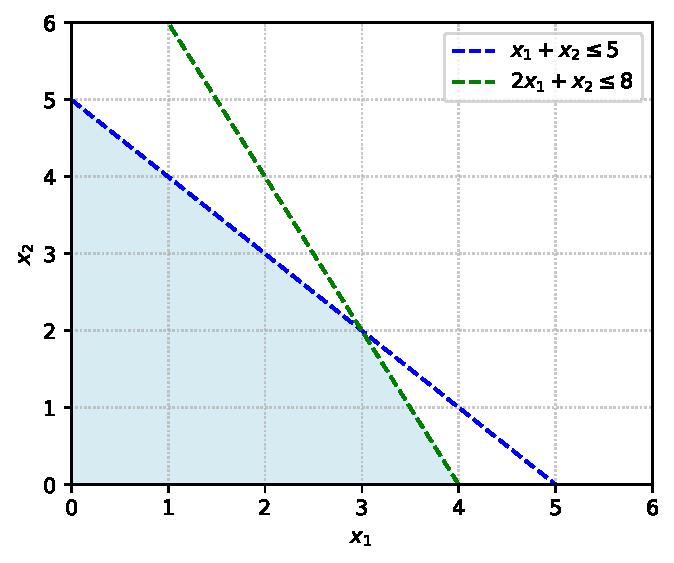
\includegraphics[keepaspectratio]{chapters/Preliminares_files/figure-pdf/fig-poliedro-output-1.pdf}}

}

\caption{\label{fig-poliedro}Representación gráfica de un poliedro
convexo en \(\mathbb{R}^2\), definido por el sistema de desigualdades
lineales \(x_1 + x_2 \leq 5\), \(2x_1 + x_2 \leq 8\), \(x_1 \geq 0\),
\(x_2 \geq 0\). La región factible, sombreada en azul claro, corresponde
al conjunto de soluciones admisibles para un subproblema de asignación
de inventario o flujo en un modelo de localización--inventario. Su
estructura poliédrica refleja la linealidad de las restricciones de
capacidad, cobertura de demanda y no negatividad, y garantiza convexidad
cuando las decisiones de apertura de almacenes están fijas.}

\end{figure}%

\begin{itemize}
\tightlist
\item
  \textbf{Conjunto cerrado en dimensión finita}: En \(\mathbb{R}^n\) con
  la topología euclidiana, un conjunto es \textbf{cerrado} si contiene
  todos sus puntos límite. Todo subespacio vectorial de \(\mathbb{R}^n\)
  es cerrado, y en dimensión finita, los conjuntos cerrados y acotados
  son compactos (teorema de Heine--Borel). Esta propiedad es clave para
  garantizar existencia de soluciones en optimización.
\end{itemize}

\section{Funciones y propiedades analíticas}\label{sec-funcion_CD}

Las propiedades analíticas de la función objetivo como su
diferenciabilidad, curvatura (Hessiano) y estructura (separabilidad,
convexidad) determinan directamente la elección del método de solución,
la calidad de las soluciones obtenidas y la eficiencia computacional del
proceso de optimización. En el contexto de la logística humanitaria bajo
incertidumbre, la función de costo total combina términos no lineales
(como el inventario de seguridad basado en la distribución normal) con
decisiones discretas (por ejemplo, abrir o no un almacén), lo que da
lugar a un paisaje no convexo y no separable. Aun así, comprender
propiedades locales como la suavidad del gradiente o la
Lipschitz-continuidad del Hessiano permite aplicar métodos iterativos
robustos (por ejemplo, L-BFGS-B) y garantizar su convergencia. Además,
cuando se fijan las decisiones discretas (es decir, se decide qué
almacenes están abiertos), el problema restante suele ser fuertemente
convexo o casi separable, lo que facilita el diseño de algoritmos
eficientes y el análisis de sensibilidad.

La formulación del costo total en inventario humanitario depende de
propiedades analíticas que facilitan el análisis de optimalidad:

\begin{itemize}
\tightlist
\item
  \textbf{Función continuamente diferenciable}: Una función
  \(f: \mathbb{R}^n \to \mathbb{R}\) es \textbf{continuamente
  diferenciable} en un conjunto abierto
  \(\mathcal{U} \subseteq \mathbb{R}^n\) si todas sus derivadas
  parciales existen y son funciones continuas en \(\mathcal{U}\). En
  este caso, se dice que \(f \in C^1(\mathcal{U})\). Esta propiedad
  garantiza que el gradiente \(\nabla f(x)\) varía suavemente en
  \(\mathcal{U}\), lo cual es esencial para la convergencia de métodos
  iterativos como el gradiente descendente y para la validez de las
  condiciones de optimalidad de primer orden (Nocedal y Wright (2006),
  Sección 2.1).
\item
  \textbf{Hessiano}: Dada una función \(f: \mathbb{R}^n \to \mathbb{R}\)
  dos veces continuamente diferenciable en un conjunto abierto
  \(\mathcal{U} \subseteq \mathbb{R}^n\), su \textbf{matriz Hessiana} (o
  simplemente \textbf{Hessiano}) en un punto \(x \in \mathcal{U}\) es la
  matriz simétrica de segundas derivadas parciales: \[
  \nabla^2 f(x) = \left[ \frac{\partial^2 f}{\partial x_i \partial x_j}(x) \right]_{i,j=1}^n.
  \] El Hessiano describe la curvatura local de \(f\) y es fundamental
  en el análisis de segundo orden, en la caracterización de mínimos
  locales y en métodos de optimización como Newton o cuasi-Newton. Si
  \(\nabla^2 f(x) \succ 0\) (definida positiva), entonces \(x\) es un
  mínimo local estricto bajo condiciones de primer orden.

  \begin{itemize}
  \tightlist
  \item
    \textbf{Hessiano Lipschitz-continuo}: Sea
    \(f: \mathbb{R}^n \to \mathbb{R}\) una función dos veces
    continuamente diferenciable en un conjunto abierto
    \(\mathcal{U} \subseteq \mathbb{R}^n\). Se dice que su
    \textbf{Hessiano \(\nabla^2 f\) es Lipschitz-continuo} en
    \(\mathcal{U}\) si existe una constante \(L_H > 0\) tal que\\
    \[
    \|\nabla^2 f(x) - \nabla^2 f(y)\| \leq L_H \|x - y\|, \quad \forall x, y \in \mathcal{U},
    \] donde \(\|\cdot\|\) denota una norma matricial compatible (por
    ejemplo, la norma espectral). Esta propiedad garantiza que la
    curvatura de \(f\) no varía de forma abrupta y es clave para
    establecer tasas de convergencia superlineal o cuadrática en métodos
    de segundo orden, como Newton o BFGS (Nocedal y Wright (2006),
    Sección 6.4).
  \item
    \textbf{Función cuadrática fuertemente convexa}: Una función
    \(f: \mathbb{R}^n \to \mathbb{R}\) es \textbf{cuadrática fuertemente
    convexa} si puede escribirse como\\
    \[
    f(x) = \tfrac{1}{2} x^\top Q x - b^\top x + c,
    \]\\
    donde \(Q \in \mathbb{R}^{n \times n}\) es una matriz
    \textbf{simétrica y definida positiva} (\(Q \succ 0\)),
    \(b \in \mathbb{R}^n\) y \(c \in \mathbb{R}\). La condición
    \(Q \succ 0\) implica que existe una constante \(\mu > 0\) tal que\\
    \[
    x^\top Q x \geq \mu \|x\|^2, \quad \forall x \in \mathbb{R}^n,
    \]\\
    lo que garantiza que \(f\) tiene un único mínimo global y que su
    paisaje de optimización es ``bien condicionado''. Esta propiedad es
    fundamental para asegurar convergencia rápida de métodos iterativos
    como el gradiente descendente o BFGS.
  \end{itemize}
\item
  \textbf{Función convexa}: \(f: \mathbb{R}^n \to \mathbb{R}\) es
  convexa si\\
  \[
  f(\lambda x + (1-\lambda)y) \leq \lambda f(x) + (1-\lambda)f(y), \quad \forall x,y, \lambda \in [0,1].
  \] La convexidad garantiza que todo mínimo local sea global, una
  propiedad deseable en diseño de redes.
\item
  \textbf{Función estrictamente cuadrática}:
  \(f(x) = \tfrac{1}{2} x^\top Q x - b^\top x + c\), con
  \(Q \in \mathbb{R}^{n \times n}\) simétrica. Si \(Q\) es constante, el
  Hessiano \(\nabla^2 f(x) = Q\) también lo es, lo que simplifica el
  análisis de curvatura en modelos de costo.
\item
  \textbf{Direcciones conjugadas}: Dada una matriz simétrica definida
  positiva \(Q \in \mathbb{R}^{n \times n}\), un conjunto de vectores no
  nulos \(\{p_0, p_1, \dots, p_{k}\} \subseteq \mathbb{R}^n\) es
  \textbf{\(Q\)-conjugado} (o \textbf{conjugado respecto a \(Q\)}) si\\
  \[
  p_i^\top Q p_j = 0, \quad \forall i \neq j.
  \] En el contexto de minimización de una función cuadrática
  \(f(x) = \tfrac{1}{2} x^\top Q x - b^\top x + c\), las direcciones
  conjugadas permiten alcanzar el mínimo global en a lo sumo \(n\)
  iteraciones, ya que exploran subespacios mutuamente ortogonales en la
  métrica inducida por \(Q\). Los métodos de la familia de Broyden
  (incluyendo BFGS y DFP) generan tales direcciones cuando se aplican a
  funciones cuadráticas con búsquedas lineales exactas.

  \begin{itemize}
  \tightlist
  \item
    \textbf{Rapidez de convergencia}: Sea \(\{x_k\}\) una sucesión que
    converge a un punto \(x^\star\). La \textbf{rapidez de convergencia}
    describe qué tan rápido \(\|x_k - x^\star\|\) tiende a cero cuando
    \(k \to \infty\). Las tasas más comunes son:
  \item
    \textbf{Lineal}: existe \(r \in (0,1)\) tal que\\
    \[
      \limsup_{k \to \infty} \frac{\|x_{k+1} - x^\star\|}{\|x_k - x^\star\|} \leq r.
      \]
  \item
    \textbf{Superlineal}:\\
    \[
      \lim_{k \to \infty} \frac{\|x_{k+1} - x^\star\|}{\|x_k - x^\star\|} = 0.
      \]
  \item
    \textbf{Cuadrática}: existe \(C > 0\) tal que\\
    \[
      \limsup_{k \to \infty} \frac{\|x_{k+1} - x^\star\|}{\|x_k - x^\star\|^2} \leq C.
      \] Estas definiciones permiten comparar la eficiencia asintótica
    de métodos iterativos (Nocedal y Wright (2006), Sección 2.3).
  \end{itemize}
\item
  \textbf{Separabilidad}: \(f(x)\) es separable si puede escribirse como
  \(f(x) = \sum_{i=1}^n f_i(x_i)\). Esta propiedad permite descomponer
  el problema en subproblemas independientes, útil en redes con nodos
  débilmente acoplados. La función de costo \textbf{no es separable},
  debido a la interacción entre tamaño de lote, inventario de seguridad
  y penalización por faltantes.
\end{itemize}

\begin{figure}

\centering{

\pandocbounded{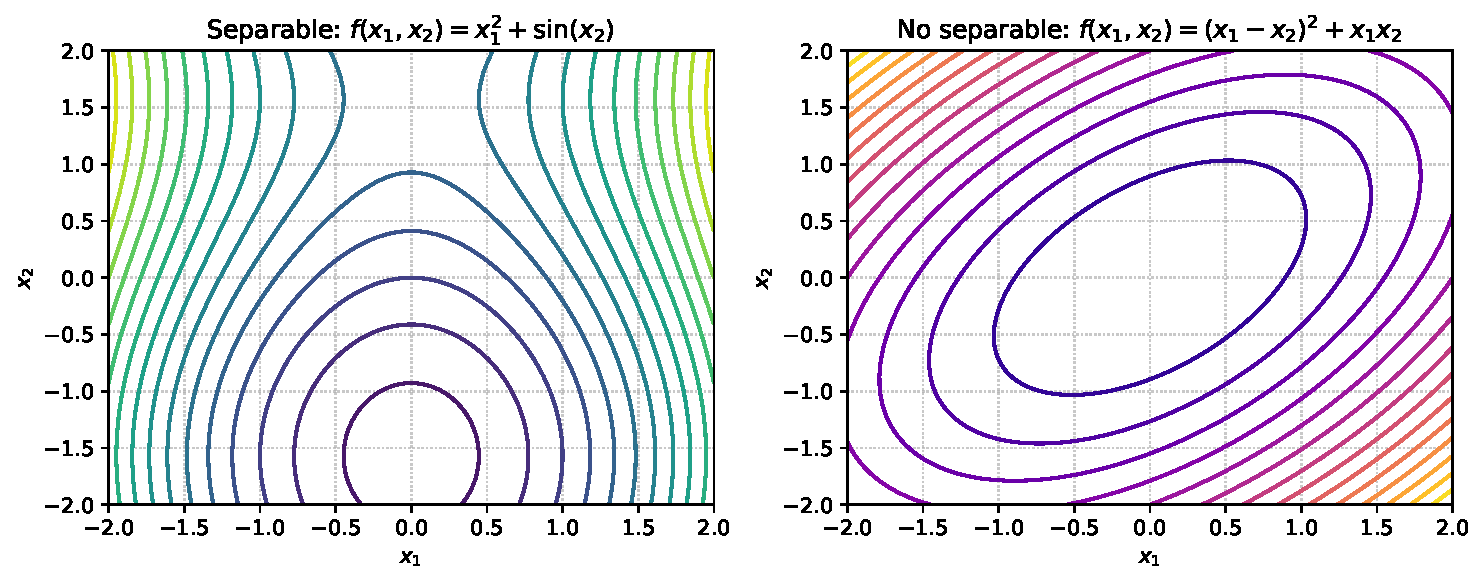
\includegraphics[keepaspectratio]{chapters/Preliminares_files/figure-pdf/fig-separable-output-1.pdf}}

}

\caption{\label{fig-separable}Comparación entre una función separable y
una no separable mediante curvas de nivel. A la izquierda,
\(f(x_1,x_2) = x_1^2 + \sin(x_2)\) es separable, pues su estructura no
acopla las variables: las curvas de nivel son alineadas con los ejes, lo
que permite optimización por coordenadas. A la derecha,
\(f(x_1,x_2) = (x_1 - x_2)^2 + x_1 x_2\) es no separable, con curvas
inclinadas que reflejan interacción entre decisiones una característica
clave en modelos de inventario humanitario, donde el tamaño del lote, el
inventario de seguridad y la penalización por faltantes están
fuertemente acoplados.}

\end{figure}%

\section{Matrices definidas positivas y su papel en la
optimización}\label{matrices-definidas-positivas-y-su-papel-en-la-optimizaciuxf3n}

En optimización de funciones en varias variables, la \textbf{matriz
Hessiana} \(\nabla^2 f(x)\) describe la curvatura local de la función
objetivo \(f\). Una propiedad fundamental es si esta matriz es
\textbf{definida positiva}, lo cual se denota como
\(\nabla^2 f(x) \succ 0\).

Formalmente, una matriz simétrica \(A \in \mathbb{R}^{n \times n}\) es
\textbf{definida positiva} si\\
\[
x^\top A x > 0 \quad \text{para todo } x \in \mathbb{R}^n,\ x \neq 0.
\]

Esta condición garantiza que la función \(f\) es \textbf{estrictamente
convexa} en una vecindad del punto \(x\), y por tanto, si además
\(\nabla f(x) = 0\), entonces \(x\) es un \textbf{mínimo local
estricto}. En modelos de inventario humanitario, donde la función de
costo incluye términos cuadráticos o aproximaciones de segundo orden
(por ejemplo, en el cálculo del inventario de seguridad bajo demanda
normal), la definición positiva del Hessiano en un punto crítico
garantiza que dicho punto es un mínimo local estricto y asegura la
convergencia local de los métodos basados en curvatura, como Newton o
L-BFGS. No obstante, la unicidad de la solución óptima no se deduce
únicamente de esta propiedad puntual, sino que requiere hipótesis
globales adicionales, como la convexidad estricta de la función objetivo
en todo el conjunto factible.

\section{Estructura general de problemas de optimización con
restricciones}\label{sec-bigM}

Los modelos de logística humanitaria integran decisiones de naturaleza
distinta: \textbf{estratégicas} (por ejemplo, dónde ubicar centros de
distribución) y \textbf{tácticas/operativas} (como cuánto inventario
almacenar o cuánta ayuda enviar). Esta combinación da lugar a problemas
de optimización \textbf{mixtos}, que involucran variables binarias (para
las decisiones de apertura/cierre) y variables continuas no negativas
(para flujos, inventarios o asignaciones).

En términos generales, el problema puede expresarse como:

\[
\begin{aligned}
\min_{x,y} \quad & f(x, y) \\
\text{sujeto a} \quad & g_i(x, y) \leq 0, \quad i = 1,\dots,m, \\
& x \in \{0,1\}^p, \quad y \in \mathbb{R}_+^q,
\end{aligned}
\]

donde \(f\) representa el costo total esperado (incluyendo
penalizaciones por faltantes y costos de operación), y las restricciones
modelan capacidades, cobertura de demanda y lógica de activación.

Un componente esencial de esta estructura es la \textbf{vinculación
entre variables discretas y continuas}, comúnmente implementada mediante
la \textbf{formulación big-M}:

\begin{itemize}
\tightlist
\item
  \textbf{Formulación big-M estándar}: restricción de la forma
  \(y \leq M x\), con \(x \in \{0,1\}\), \(y \in \mathbb{R}_+\), y
  \(M > 0\) suficientemente grande, usada para modelar la implicación
  lógica \(x = 0 \Rightarrow y = 0\). Por ejemplo, si no se abre un
  almacén (\(x = 0\)), no puede enviar ayuda (\(y = 0\)).
\end{itemize}

Esta estructura mixta introduce no convexidad y discontinuidad en el
espacio de decisiones, lo que impide el uso directo de métodos basados
en gradientes y motiva el uso de algoritmos especializados, como los
discutidos en el Capítulo 5.

\section{Teoría de probabilidad y variables
aleatorias}\label{sec-variables}

En la logística humanitaria, la demanda de ayuda especialmente durante o
después de eventos como inundaciones es inherentemente incierta y
altamente variable. Modelar esta incertidumbre de forma adecuada es
crucial: usar únicamente valores promedio ignora la posibilidad de
eventos extremos, lo que puede llevar a niveles insuficientes de
inventario y, en consecuencia, a faltantes críticos. Para abordar este
desafío sin comprometer la tratabilidad del modelo de optimización, en
este trabajo se emplean herramientas de la teoría de probabilidad
\textbf{de forma previa} para caracterizar estadísticamente la demanda.
Esta caracterización permite obtener estimaciones puntuales (demanda
esperada y varianza) y derivar factores de seguridad (\(Z_{\sigma}\)),
los cuales se incorporan posteriormente como parámetros fijos y
deterministas en la formulación. De esta forma, se cuantifica tanto la
magnitud esperada como la variabilidad y el riesgo asociado a las colas
de la distribución (eventos raros pero severos), aspectos esenciales
para el cálculo del inventario de seguridad y la toma de decisiones
robustas dentro de un marco determinista

\begin{itemize}
\tightlist
\item
  \textbf{Variable aleatoria (v.a.) absolutamente continua}:
  \(\mathbb{P}(X \in A) = \int_A f_X(x)\,dx\), donde \(f_X\) es la
  densidad respecto a la medida de Lebesgue. Esta formulación es
  esencial para modelar demandas con distribuciones suaves, como la
  normal.
\item
  \textbf{Distribución normal}: si
  \(D_L \sim \mathcal{N}(\mu_L, \sigma_L^2)\), su densidad es\\
  \[
  \phi_{D_L}(d) = \frac{1}{\sqrt{2\pi}\sigma_L} \exp\!\left(-\frac{(d - \mu_L)^2}{2\sigma_L^2}\right).
  \] Esta distribución se usa para aproximar la demanda durante el
  tiempo de entrega, lo que permite calcular el inventario de seguridad.
\item
  \textbf{Varianza}: para una v.a. \(X\),
  \(\operatorname{Var}(X) = \mathbb{E}[(X - \mathbb{E}[X])^2]\). La
  varianza cuantifica la incertidumbre en la demanda; ignorarla (por
  ejemplo, al usar solo \(\mathbb{E}[d_j]\)) puede inducir soluciones
  frágiles en eventos extremos.
\end{itemize}

\begin{figure}

\centering{

\pandocbounded{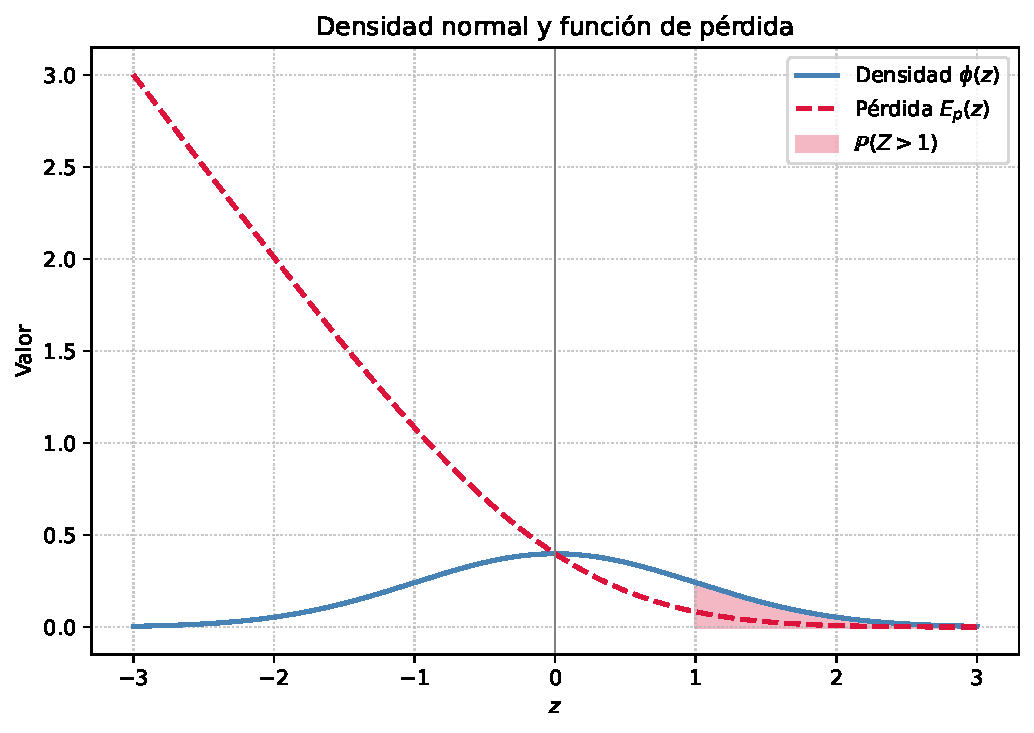
\includegraphics[keepaspectratio]{chapters/Preliminares_files/figure-pdf/fig-normal-perdida-output-1.pdf}}

}

\caption{\label{fig-normal-perdida}Función de densidad de probabilidad
\(\phi(z)\) y función de pérdida logística
\(E_p(z) = z(\Phi(z)-1) + \phi(z)\) asociadas a la distribución normal
estándar. La densidad \(\phi(z)\) (azul sólido) modela la incertidumbre
en la demanda estandarizada, mientras que la función de pérdida
\(E_p(z)\) (rojo punteado) cuantifica el déficit esperado normalizado
cuando el nivel de inventario es insuficiente (\(z < 0\)). La región
sombreada para \(z \geq 1\) ilustra la probabilidad de cola superior,
relevante para el cálculo del inventario de seguridad en contextos
humanitarios. Esta función es fundamental para internalizar el riesgo de
faltantes en la formulación del costo total.}

\end{figure}%

\begin{itemize}
\tightlist
\item
  \textbf{Notación \(\ll\)}: indica que una cantidad es mucho menor que
  otra. Por ejemplo, en la Sección~\ref{sec-impacto} se muestra que, si
  se ignora la incertidumbre en \(L\), la varianza estimada puede ser
  \(80 \ll 10\,080\), subestimando severamente el riesgo.
\end{itemize}

El \textbf{valor esperado} \(\mathbb{E}[d_j]\) representa la demanda
media en la localidad \(j\). Aunque es común usarlo como estimador
puntual en modelos deterministas, como se advierte en la
Sección~\ref{sec-determinista}, esta simplificación puede ser inadecuada
en logística humanitaria, donde la cola de la distribución (eventos
extremos) es crítica.

\section{Optimización no lineal y condiciones de
optimalidad}\label{sec-kkt}

El problema de localización--inventario analizado en este trabajo da
lugar a un modelo de optimización no lineal determinista. Aunque en la
Sección~\ref{sec-variables} se introducen conceptos de teoría de
probabilidad y variables aleatorias, estos se emplean exclusivamente
para fundamentar la obtención paramétrica de los insumos del modelo
(demanda esperada, varianza y factor de seguridad \(Z_{\sigma}\)). La
incertidumbre no se representa mediante variables aleatorias ni
formulaciones estocásticas dentro del problema de optimización; en su
lugar, se internaliza de forma fija y determinista en los coeficientes
de la función objetivo. Bajo esta estructura, las \textbf{condiciones de
Karush--Kuhn--Tucker (KKT)} proporcionan un marco teórico fundamental
para caracterizar puntos candidatos a óptimos locales, siempre que se
satisfagan ciertas condiciones de regularidad (calificación de
restricciones). Sin embargo, dado que el problema incluye variables
binarias y acoplamiento no lineal entre decisiones, el espacio factible
es \textbf{no convexo y discontinuo}, lo que implica que las condiciones
KKT aunque necesarias \textbf{no garantizan optimalidad global}. Esta
limitación justifica el uso de métodos de solución especializados, como
algoritmos de ramificación o heurísticas híbridas, que se discuten en
capítulos posteriores.

\begin{itemize}
\tightlist
\item
  \textbf{Condiciones de Karush--Kuhn--Tucker (KKT)}: condiciones
  necesarias de optimalidad local bajo restricciones de desigualdad y
  calificación de restricciones. Como se expone en Lewis y Overton
  (2013), estas condiciones \textbf{no garantizan optimalidad global} en
  problemas no convexos, como el propuesto, donde la no convexidad surge
  de las variables binarias y la no linealidad en la incertidumbre.
\end{itemize}

\bookmarksetup{startatroot}

\chapter{Fundamentación Teórica y Formulación Matemática del
Modelo}\label{fundamentaciuxf3n-teuxf3rica-y-formulaciuxf3n-matemuxe1tica-del-modelo}

\section{Introducción al problema integrado de localización e
inventario}\label{sec-problemas}

\subsection{Relevancia en logística humanitaria y gestión de
emergencias}\label{sec-problema}

La logística humanitaria desempeña un papel fundamental en la respuesta
a desastres, al coordinar la disponibilidad, distribución y acceso
equitativo a bienes esenciales en entornos caracterizados por alta
incertidumbre, infraestructura comprometida y recursos limitados (Balcik
y Beamon (2008); Caunhye, Nie, y Pokharel (2012)). A diferencia de los
sistemas logísticos comerciales, donde predominan criterios de
eficiencia económica, los contextos humanitarios priorizan objetivos de
\textbf{rapidez, cobertura universal y mitigación del riesgo}, lo que
exige modelos matemáticos capaces de integrar decisiones estratégicas y
tácticas bajo condiciones de información imperfecta.

En este marco, el \textbf{problema integrado de localización e
inventario} se ha consolidado como una herramienta clave para la
planificación anticipada, ya que permite determinar, de manera conjunta:

\begin{enumerate}
\def\labelenumi{\arabic{enumi}.}
\tightlist
\item
  \textbf{La ubicación óptima de almacenes de preposicionamiento}, y\\
\item
  \textbf{Los niveles de inventario que deben almacenarse antes de la
  ocurrencia de un evento disruptivo}.
\end{enumerate}

Ambas decisiones condicionan el desempeño global del sistema en términos
de costo total, robustez operativa y equidad en la atención. Su
naturaleza híbrida, estratégica (ubicación) y táctica (inventario),
impone desafíos estructurales que no pueden abordarse mediante enfoques
secuenciales o modelos clásicos aislados.

Aunque la demanda en estos escenarios es inherentemente incierta, en
este trabajo se adopta un \textbf{enfoque determinista robusto},
ampliamente fundamentado en la teoría de inventarios bajo demanda
aleatoria del artículo seminal Hadley y Whitin (1963). Este enfoque no
modela la incertidumbre mediante variables aleatorias ni formulaciones
estocásticas, sino que la \textbf{incorpora de forma paramétrica}
mediante un \textbf{stock de seguridad fijo}, derivado de estimaciones
de la variabilidad de la demanda.

Específicamente, se asume que la demanda en cada localidad
\(j\in\mathcal{J}\) posee un valor esperado \(d_j>0\) y una desviación
estándar \(\sigma_j\geq0\), ambos tratados como \textbf{parámetros
exógenos conocidos}. Dado un tiempo de reposición \(L>0\) y un nivel de
servicio objetivo \(\alpha\in(0,1)\), se define el \textbf{factor de
seguridad} como \(Z=\Phi^{-1}(\alpha)\), donde \(\Phi^{-1}\) denota la
inversa de la función de distribución acumulada de la normal estándar.
Aunque esta construcción se fundamenta en la teoría de probabilidad, en
la etapa de optimización dichos valores se fijan como constantes. De
este modo, se adopta una aproximación determinista basada en cuantiles
de una distribución. Este enfoque permite formular un modelo de
optimización no lineal determinista, donde el término
\(Z\sigma\sqrt{L}\) se incorpora como un parámetro exógeno que
internaliza la magnitud de la incertidumbre sin introducir variables
aleatorias ni operadores de esperanza dentro de la función objetivo.

Este enfoque permite formular un \textbf{modelo de optimización no
lineal determinista}, cuya estructura matemática se preserva intacta
frente a la complejidad computacional inherente a los modelos
estocásticos. La ausencia de esperanzas, escenarios o variables de
segundo nivel garantiza trazabilidad analítica, estabilidad numérica y
compatibilidad con métodos de optimización eficientes para problemas con
cotas, como se discutirá en capítulos posteriores.

\subsection{Limitaciones de los enfoques clásicos bajo incertidumbre y
no linealidad}\label{sec-Nolinealidad}

Los modelos clásicos de localización e inventario, como el Uncapacitated
Facility Location Problem (UFLP) y el Economic Order Quantity (EOQ)
model o sus variantes deterministas, han sido ampliamente estudiados
bajo el supuesto de \textbf{información perfecta y estructura lineal},
un enfoque cuya pertinencia disminuye notablemente en escenarios
humanitarios caracterizados por \textbf{incertidumbre estructural} y
\textbf{no linealidad inherente} en costos y restricciones como se
representa en Hadley y Whitin (1963); Snyder (2006).

\subsubsection{Supuestos restrictivos del modelo EOQ
clásico}\label{supuestos-restrictivos-del-modelo-eoq-cluxe1sico}

El modelo EOQ se fundamenta en supuestos como:

\begin{enumerate}
\def\labelenumi{\arabic{enumi}.}
\tightlist
\item
  Demanda constante y conocida: \(D > 0\) (unidades por unidad de
  tiempo).
\item
  Tiempo de entrega determinista y conocido: \(L \geq 0\).
\item
  Costos lineales y constantes: costo fijo por pedido \(S > 0\), costo
  unitario de mantenimiento de inventario \(H > 0\), y costo unitario de
  adquisición \(C > 0\). No se permiten faltantes.
\item
  Reposición instantánea y sin restricciones de capacidad, de acuerdo
  con los supuestos planteados por Hadley y Whitin (1963).
\end{enumerate}

Bajo estos supuestos, la función de costo total promedio por unidad de
tiempo se expresa como:

\[
Z^{EOQ}(Q)=\frac{D}{Q}S+\frac{Q}{2}H+DC,
\]

donde:

\begin{itemize}
\tightlist
\item
  \(Q > 0\) es el tamaño del lote o cantidad de pedido (variable de
  decisión continua),
\item
  \(D\) es la demanda esperada por periodo de planificación,
\item
  \(S\) es el costo fijo asociado a la emisión de cada pedido,
\item
  \(H\) es el costo unitario de mantener una unidad en inventario por
  unidad de tiempo,
\item
  \(C\) es el costo unitario de adquisición del producto.
\end{itemize}

La minimización de esta función conduce a la solución óptima clásica:

\[
Q^{EOQ}=\sqrt{\frac{2DS}{H}}.
\]

Este resultado depende de la \textbf{deterministicidad} y la
\textbf{convexidad estricta}. Sin embargo, en logística humanitaria:

\begin{itemize}
\tightlist
\item
  La demanda es aleatoria \(D(\omega)\).
\item
  \(L\) es incierto debido a afectaciones en infraestructura.
\item
  Los faltantes deben modelarse mediante una penalización finita
  \(\beta>0\).
\item
  Los costos pueden presentar economías de escala y no convexidades, es
  decir, situaciones donde el costo promedio por unidad disminuye al
  aumentar el volumen de pedido o transporte, como se discute en Porteus
  (2002).
\end{itemize}

\subsubsection{Incapacidad del EOQ para capturar riesgo}\label{sec-ZEOQ}

Aunque la demanda en contextos humanitarios es inherentemente
estocástica, en este trabajo se adopta un enfoque determinista robusto,
ampliamente utilizado en la teoría de inventarios bajo incertidumbre
como se expone en Porteus (2002) y Zipkin (2000). Bajo los supuestos
clásicos de demanda normal durante el tiempo de entrega, política de
revisión continua y costo lineal por faltante, el costo total esperado
puede aproximarse mediante una función determinista del tamaño de lote
\(Q\). Esta aproximación incorpora los efectos de la incertidumbre a
través del inventario de seguridad \(Z_\alpha \sigma_L\) y la
penalización esperada por faltantes, pero su optimización se realiza
como un problema determinista.

Si la demanda durante el tiempo de entrega se modela como
\(D_L \sim \mathcal{N}(\mu_L, \sigma_L^2)\), el nivel de inventario debe
satisfacer: \[
\mathbb{P}(D_L \leq Q/2 + Z_\alpha \sigma_L) \geq \alpha,
\]

lo que justifica la inclusión del término \(Z_\alpha \sigma_L\) en la
función de costo. Con ello, la función de costo extendida adopta la
forma: Con ello, la función de costo extendida se vuelve:

\begin{equation}\phantomsection\label{eq-Zq}{
Z(Q)=\frac{D}{Q}S+\left(\frac{Q}{2}+Z_\alpha\sigma_L\right)H+DC+\frac{D}{Q}\beta C. 
}\end{equation}

Esta función \textbf{no es convexa globalmente} cuando \(\sigma_L\)
depende de \(Q\), como ocurre cuando existe congestión en transporte o
variabilidad dependiente del tamaño del pedido, aspectos estudiados por
Bertsimas y Thiele (2006) y Shapiro, Dentcheva, y Ruszczyński (2021).

\begin{quote}
\textbf{Proposición (No linealidad estricta).}\\
La función \(Z(Q)\) definida en Sección~\ref{sec-ZEOQ} es diferenciable
en \((0,\infty)\), pero no es convexa globalmente (ver
Sección~\ref{sec-funcion_CD}) si \(\beta>0\) y \(\sigma_L>0\).\\
Si \(\sigma_L\) es constante: \[
\frac{d^2 Z}{dQ^2}=\frac{2D(S+\beta C)}{Q^3}>0.
\] Pero si \(\sigma_L=\sigma\sqrt{L(Q)}\) y \(L(Q)\) es no lineal,
entonces \(Z(Q)\) pierde convexidad.
\end{quote}

Esto demuestra que muchos métodos clásicos basados en convexidad y
separabilidad (ver Sección~\ref{sec-funcion_CD}) resultan inaplicables
en condiciones realistas.

\subsubsection{Limitaciones de modelos de localización
deterministas}\label{sec-determinista}

El modelo clásico UFLP resuelve:

\[
\min_{x\in\{0,1\}^m, y\ge 0}\sum_{i}f_i x_i + \sum_{i}\sum_j c_{ij}y_{ij},
\]

bajo restricciones de asignación deterministas. Sin embargo:

\begin{itemize}
\tightlist
\item
  La demanda \(d_j\) es aleatoria.
\item
  Los costos pueden variar según accesibilidad o daños.
\item
  Las capacidades reales son inciertas.
\end{itemize}

Modelar \(d_j\) mediante \(\mathbb{E}[d_j]\) genera soluciones frágiles
frente a escenarios adversos Snyder (2006).

\subsubsection{Ejemplo ilustrativo: EOQ clásico vs.~EOQ extendido con
stock de seguridad y
penalización}\label{ejemplo-ilustrativo-eoq-cluxe1sico-vs.-eoq-extendido-con-stock-de-seguridad-y-penalizaciuxf3n}

Considérese un contexto en el que la demanda esperada es \(D=1000\)
unidades, con una variabilidad estimada cuya desviación estándar es
\(\sigma=10\). Aunque la demanda real puede fluctuar (por ejemplo, entre
800 y 1200 unidades en eventos históricos), en este enfoque se modela la
incertidumbre mediante parámetros fijos derivados de su comportamiento
estadístico. Los demás parámetros son:

\begin{itemize}
\tightlist
\item
  Costo de pedido: \(S=100\)\\
\item
  Costo unitario de mantenimiento: \(H=5\)\\
\item
  Costo unitario de adquisición: \(C=10\)\\
\item
  Penalización por faltante: \(\beta=50\)\\
\item
  Tiempo de reposición: \(L=0.1\)\\
\item
  Nivel de servicio objetivo: \(95\%\Rightarrow Z_{\alpha}=1.645\)
\end{itemize}

El stock de seguridad se calcula como:

\[
SS=Z_{\alpha}\sigma\sqrt{L}\approx1.645\cdot10\cdot\sqrt{0.1}\approx5.20,
\]

aunque en la función de costo extendida, este valor se incorpora como un
término constante.

\subsubsection{EOQ clásico (ignora incertidumbre y
faltantes)}\label{eoq-cluxe1sico-ignora-incertidumbre-y-faltantes}

\[
Q_{EOQ}=\sqrt{\frac{2DS}{H}}=\sqrt{\frac{2(1000)(100)}{5}}=200,
\]

y su costo asociado es:

\[
Z_{EOQ}=\frac{200}{1000}\cdot100+\frac{2}{200}\cdot5+1000\cdot10
=500+500+10000=11000.
\]

\subsubsection{EOQ extendido (con stock de seguridad y penalización por
faltantes)}\label{eoq-extendido-con-stock-de-seguridad-y-penalizaciuxf3n-por-faltantes}

La función de costo adopta la forma:

\[
Z(Q)=\frac{Q}{D}(S+\beta C)+\left(\frac{2}{Q}+Z_{\alpha}\sigma\sqrt{L}\right)H+DC.
\]

Sustituyendo los valores:

\begin{align*}
Z(Q) &= \frac{Q}{1000}(100+500) + \left(\frac{2}{Q} + 5.20\right)\cdot 5 + 10000 \\
     &= \frac{Q}{600000} + 2.5Q + 10026.
\end{align*}

Minimizando esta función determinista:

\[
Q^{\ast}=\sqrt{\frac{2.5}{600000}}\approx489.9,\qquad
Z(Q^{\ast})\approx12475.44.
\]

Si, por error, se usara la política del EOQ clásico (\(Q=200\)):

\[
Z(200)=\frac{200}{600000}+2.5\cdot200+10026
=3000+500+10026=13526,
\]

lo que representa un \textbf{8.4\% más de costo} respecto a la política
óptima del modelo extendido, además de una \textbf{exposición
significativamente mayor al riesgo de faltante}.

Este contraste demuestra que los modelos deterministas que ignoran la
variabilidad de la demanda y los costos de faltante pueden producir
políticas subóptimas o inadmisibles en contextos humanitarios, donde la
insatisfacción de la demanda tiene consecuencias operativas y éticas
relevantes.

\subsection{Estructura híbrida: decisiones discretas (ubicación) y
continuas
(inventario)}\label{estructura-huxedbrida-decisiones-discretas-ubicaciuxf3n-y-continuas-inventario}

Los problemas integrados de localización e inventario pertenecen a la
clase de \textbf{modelos de optimización mixta}, en los que coexisten
variables discretas (por ejemplo, decisiones binarias de apertura de
almacenes) y variables continuas (como flujos de asignación o niveles de
inventario). Esta combinación induce una \textbf{estructura no convexa y
no conexa en el conjunto factible}, debido a la naturaleza combinatoria
de las variables binarias.

Como argumentan Wolsey (1998), Grossmann (2002) y Daskin (2013), esta
pérdida de convexidad impide la aplicación directa de técnicas clásicas
de optimización convexa, tales como las condiciones de
Karush--Kuhn--Tucker (KKT Sección~\ref{sec-kkt}) para garantizar
optimalidad global, y exige el uso de métodos especializados para
problemas mixtos entero-continuos.

\subsubsection{Formulación matemática del espacio de
decisiones}\label{sec-noconvexidad}

Sea:

\begin{itemize}
\tightlist
\item
  \(\mathcal{I} = \{1,\ldots,m\}\) el conjunto de ubicaciones posibles
  para almacenes,
\item
  \(\mathcal{J} = \{1,\ldots,n\}\) las localidades de demanda,
\item
  \(x = (x_1,\dots,x_m)^\top \in \{0,1\}^m\) las decisiones binarias de
  apertura,
\item
  \(y = (y_{ij}) \in \mathbb{R}_+^{m\times n}\) los flujos desde
  almacenes a localidades,
\item
  \(s = (s_1,\dots,s_m)^\top \in \mathbb{R}_+^m\) el inventario
  preposicionado.
\end{itemize}

El espacio factible se define como el conjunto:

\begin{equation}\phantomsection\label{eq-EF}{
\mathcal{X} := \left\{ (x, y, s) \;\middle|\;
\begin{aligned}
& x_i \in \{0,1\}, && \forall i \in \mathcal{I}, \\
& y_{ij} \ge 0,    && \forall i \in \mathcal{I},\; \forall j \in \mathcal{J}, \\
& s_i \ge 0,       && \forall i \in \mathcal{I}, \\
& \sum_{i \in \mathcal{I}} y_{ij} \ge d_j, && \forall j \in \mathcal{J}, \\
& \sum_{j \in \mathcal{J}} y_{ij} \le s_i, && \forall i \in \mathcal{I}, \\
& s_i \le M x_i,   && \forall i \in \mathcal{I}
\end{aligned}
\right\}.
}\end{equation}

Aquí, \(d_j > 0\) representa la demanda de la localidad \(j\) y \(M\) es
un parámetro de gran magnitud. La tercera restricción impone un vínculo
lógico: si \(x_i = 0\), entonces \(s_i = 0\) y, en consecuencia,
\(y_{ij} = 0\) para todo \(j \in \mathcal{J}\).

Este acoplamiento, combinado con la naturaleza \textbf{binaria} de las
variables \(x_i\), impide que el conjunto factible \(\mathcal{X}\) sea
convexo. La no convexidad se debe exclusivamente a la
\textbf{discreción} de las variables \(x_i\): el promedio de dos puntos
factibles con configuraciones distintas de infraestructura no es
factible, ya que viola la condición \(x_i \in \{0,1\}\). Esta propiedad,
la ausencia de convexidad en el conjunto factible debido a variables
enteras, es bien conocida en la teoría de optimización mixta, como puede
verse en el ejemplo de selección de proyectos presentado por Bertsekas
(1999) donde las decisiones binarias de aceptar o rechazar proyectos
generan un conjunto factible no convexo.

\begin{quote}
\textbf{Proposición (No convexidad).}\\
El conjunto \(\mathcal{X}\) definido en (Ecuación~\ref{eq-EF})
\textbf{no es convexo}.\\
\emph{Demostración.} Considérense las configuraciones factibles con
\(x^{(1)} = (1,0,\dots,0)\),
\(s^{(1)} = (d^\top \mathbf{1}, 0, \dots, 0)^\top\), \(y^{(1)}\)
asignando toda la demanda al almacén 1, y análogamente
\(x^{(2)} = (0,1,0,\dots,0)\) con asignación al almacén 2. Ambos puntos
pertenecen a \(\mathcal{X}\). Sin embargo, su punto medio tiene
\(x_i = 1/2\) para \(i=1,2\), lo cual viola \(x_i \in \{0,1\}\). Por lo
tanto, \(\mathcal{X}\) no es convexo. ∎
\end{quote}

Debido a esta no convexidad, el problema \textbf{no pertenece a la clase
de optimización convexa}, y en consecuencia \textbf{no es posible
garantizar optimalidad global mediante condiciones de optimalidad
basadas en el análisis convexo clásico}.

\subsubsection{Función objetivo y acoplamiento
estructural}\label{sec-acoplamiento}

La función objetivo del modelo de ubicación de almacenes e inventario
humanitario se define como:

\begin{equation}\phantomsection\label{eq-Z_xys}{
Z(x,y,s) 
= 
\underbrace{\sum_{i\in\mathcal{I}} f_i(x_i)}_{\text{Costos fijos}}
+ \underbrace{\sum_{i\in\mathcal{I}} h_i s_i}_{\text{Costos de inventario}}
+ \underbrace{\sum_{i\in\mathcal{I}}\sum_{j\in\mathcal{J}} c_{ij} y_{ij}}_{\text{Costos de transporte}}.
}\end{equation}

Aunque la parte en variables continuas es lineal, el término
\(f_i(x_i)\) introduce una \textbf{no linealidad discreta}, ya que
\(x_i \in \{0,1\}\). Esta discontinuidad, combinada con el acoplamiento
lógico \(s_i \leq M x_i\), da lugar a un \textbf{espacio de decisiones
no convexo y combinatorio}.

La dificultad computacional del problema se debe a la interacción entre
variables discretas y continuas, que genera una estructura no separable
y no convexa, característica de los \textbf{programas mixtos-enteros no
lineales (MINLP)}. Como señalan Grossmann (2002), esta clase de
problemas es computacionalmente exigente porque:

\begin{itemize}
\tightlist
\item
  no se puede aplicar directamente la optimización convexa,
\item
  los métodos de enumeración son inviables en problemas de tamaño
  moderado,
\item
  y la no linealidad impide el uso de técnicas eficientes basadas en
  planos de corte o relajaciones lineales exactas.
\end{itemize}

El sistema presenta una jerarquía:

\begin{enumerate}
\def\labelenumi{\arabic{enumi}.}
\tightlist
\item
  \(x\) determina la infraestructura disponible,\\
\item
  \(s\) depende de \(x\),\\
\item
  \(y\) depende de \(s\).
\end{enumerate}

Esto produce una dependencia en cascada que elimina la separabilidad
global del problema.

\begin{quote}
\textbf{Proposición (Convexidad condicional).}\\
Para cualquier \(\bar{x} \in \{0,1\}^m\), el subproblema

\[
\min_{(y,s) \in \mathcal{X}(\bar{x})} Z(\bar{x}, y, s)
\]

es un problema de programación lineal y, por tanto, convexo.\\
\emph{Demostración.} Al fijar \(\bar{x}\), los términos
\(f_i \bar{x}_i\) se convierten en constantes. La función objetivo
resultante es lineal en \((y,s)\), y todas las restricciones que definen
\(\mathcal{X}(\bar{x})\) son lineales en estas variables. Por
definición, esto constituye un problema de programación lineal, cuyo
conjunto factible es un poliedro convexo. \(\blacksquare\)
\end{quote}

Esta propiedad, consistente en \emph{la convexidad del subproblema
continuo para una configuración de apertura fija}, es fundamental para
la aplicación de métodos de descomposición, tales como el algoritmo de
Benders. En dichos enfoques, el problema original se divide en:

\begin{itemize}
\tightlist
\item
  \textbf{problema maestro}, que maneja las variables enteras (\(x\)) y
  genera configuraciones candidatas, y
\item
  un \textbf{subproblema}, que, para una configuración dada, resuelve el
  problema continuo (aquí, lineal) y devuelve información (por ejemplo,
  cortes de Benders) para refinar el problema maestro, siguiendo la
  metodología de descomposición descrita en Wolsey (1998).
\end{itemize}

\subsubsection{Ejemplo ilustrativo: interacción
discreto--continuo}\label{ejemplo-ilustrativo-interacciuxf3n-discretocontinuo}

Considérese:

\begin{itemize}
\tightlist
\item
  \(m=2\) almacenes,\\
\item
  \(n=2\) demandas con \(d_1=d_2=50\),\\
\item
  Costos fijos \(f_1=300\), \(f_2=400\),\\
\item
  Costos de inventario \(h_1=h_2=3\),\\
\item
  Costos de transporte:\\
  \(c_{11}=8\), \(c_{12}=15\),\\
  \(c_{21}=12\), \(c_{22}=7\),\\
\item
  \(M=100\).
\end{itemize}

\textbf{(i) Abrir solo 1:}\\
\[
Z = 300 + 3\cdot 100 + (8\cdot 50 + 15\cdot 50)=1750.
\]

\textbf{(ii) Abrir solo 2:}\\
\[
Z = 400 + 3\cdot 100 + (12\cdot 50 + 7\cdot 50)=1650.
\]

\textbf{(iii) Abrir ambos:}\\
Asignación eficiente, pero mayor costo fijo:\\
\[
Z = 300 + 400 + 3\cdot 100 + (8\cdot 50 + 7\cdot 50)=1750.
\]

La mejor configuración es abrir únicamente el almacén 2. Este resultado
ilustra una propiedad fundamental de los problemas que combinan
variables discretas y continuas: la solución óptima puede cambiar de
manera discontinua ante perturbaciones arbitrariamente pequeñas en los
parámetros del problema. Por ejemplo, si \(f_2\) disminuye a \(350\), la
solución óptima se mantiene; pero si \(f_1\) baja a \(250\), podría
resultar óptimo abrir el almacén \(1\).

A este fenómeno, la dependencia discontinua de la solución óptima
respecto a los datos del problema, causada por la naturaleza
combinatoria de las decisiones binarias, nos referiremos como
sensibilidad discreta. Esta característica distingue claramente a los
modelos mixtos entero-continuos de los problemas puramente continuos,
donde bajo condiciones de regularidad la solución óptima varía de forma
suave como se puede ver en Daskin (2013).

El conjunto factible de este tipo de problemas, definido por la
combinación de variables binarias y continuas junto con restricciones de
activación lógica, \textbf{no es convexo} (como se demostró en la
Sección~\ref{sec-noconvexidad}). Esta no convexidad, junto con la
interacción entre decisiones estratégicas y operativas, exige el uso de
técnicas propias de la programación entera mixta y de la optimización
combinatoria. Estas bases teóricas sustentan el modelo propuesto en las
secciones siguientes, donde se integra esta estructura con un componente
de inventario no lineal bajo incertidumbre parametrizada.

\section{Marco general de modelado: variables, parámetros y espacio de
decisión}\label{marco-general-de-modelado-variables-paruxe1metros-y-espacio-de-decisiuxf3n}

\subsection{\texorpdfstring{Conjuntos de índices: alamcenes potenciales
\(\mathcal{I}\) y localidades de demanda
\(\mathcal{J}\)}{Conjuntos de índices: alamcenes potenciales \textbackslash mathcal\{I\} y localidades de demanda \textbackslash mathcal\{J\}}}\label{conjuntos-de-uxedndices-alamcenes-potenciales-mathcali-y-localidades-de-demanda-mathcalj}

En la formulación matemática del problema integrado de localización e
inventario, los conjuntos de índices constituyen la base sobre la cual
se definen las variables de decisión, los parámetros y las
restricciones. Como se estableció en la Sección~\ref{sec-problemas},
denotamos por

\begin{itemize}
\tightlist
\item
  \(\mathcal{I}\): el conjunto de \textbf{almacenes candidatos} para
  preposicionamiento, y\\
\item
  \(\mathcal{J}\): el conjunto de \textbf{localidades geográficas
  afectadas}.
\end{itemize}

Estos conjuntos son finitos, disjuntos, es decir,
\(\mathcal{I} \cap \mathcal{J} = \varnothing\), y sus elementos
desempeñan roles distintos en el modelo: los índices en \(\mathcal{I}\)
corresponden a \emph{fuentes} de suministro, mientras que los de
\(\mathcal{J}\) representan \emph{destinos} de demanda.

La cardinalidad de \(\mathcal{I}\), denotada \(m = |\mathcal{I}|\),
determina la dimensión del espacio de decisiones estratégicas. Dado que
el costo de apertura de cada almacén se modela mediante una variable
binaria \(x_i \in \{0,1\}\), el número total de configuraciones posibles
de infraestructura es \(2^m\). Esta \textbf{explosión combinatoria}
implica que, incluso para tamaños modestos de \(m\) (por ejemplo,
\(m = 30\)), el espacio discreto contiene más de \(10^9\) soluciones
factibles. En consecuencia, métodos de enumeración exhaustiva son
inviables, y se requieren algoritmos que exploten la \textbf{estructura
matemática del problema}, es decir, su formulación como un problema de
optimización con variables mixtas, función objetivo diferenciable y
restricciones acopladas, para identificar soluciones óptimas o
aproximadas en tiempo razonable.

La interacción entre \(\mathcal{I}\) y \(\mathcal{J}\) se modela
mediante variables de flujo \(y_{ij} \geq 0\), que cuantifican la
asignación de suministros desde el almacén \(i\) a la localidad \(j\).
Esta relación define una matriz de conectividad cuya densidad depende de
factores operativos como la distancia, accesibilidad y capacidades
logísticas, y que condiciona tanto la factibilidad como la complejidad
del subproblema continuo asociado a una configuración fija de almacenes.

\subsubsection{\texorpdfstring{\textbf{Ejemplo
ilustrativo}}{Ejemplo ilustrativo}}\label{ejemplo-ilustrativo}

Supóngase un escenario de planificación para respuesta a inundaciones
dividido en cinco distritos. Se identifican tres ubicaciones potenciales
para almacenes:

\begin{itemize}
\tightlist
\item
  \(i = 1\): Aeropuerto internacional,\\
\item
  \(i = 2\): Base militar,\\
\item
  \(i = 3\): Centro de distribución de una ONG.
\end{itemize}

Asimismo, se consideran cuatro zonas vulnerables:

\begin{itemize}
\tightlist
\item
  \(j = 1\): Zona ribereña,\\
\item
  \(j = 2\): Área rural,\\
\item
  \(j = 3\): Barrio urbano denso,\\
\item
  \(j = 4\): Comunidad indígena aislada.
\end{itemize}

Los conjuntos índice resultan:

\[\mathcal{I} = \{1,2,3\}, \quad 
\mathcal{J} = \{1,2,3,4\}.\]

Sobre estos conjuntos se definirán:

\begin{itemize}
\tightlist
\item
  variables binarias \(x_i \in \{0,1\}\) para cada
  \(i \in \mathcal{I}\),\\
\item
  variables continuas de flujo \(y_{ij} \ge 0\) para
  \((i,j) \in \mathcal{I} \times \mathcal{J}\),\\
\item
  parámetros exógenos como \(c_{ij}\) (costos), \(f_i\) (costos fijos) y
  \(d_j\) (demanda).
\end{itemize}

\begin{quote}
\textbf{Nota metodológica.}\\
En modelado riguroso, los conjuntos índice deben definirse antes que las
variables, dado que estas heredan su dominio directamente de aquellos.
\end{quote}

\subsection{\texorpdfstring{Variables de decisión: binarias (\(x_i\)) y
continuas
(\(y_{ij}\))}{Variables de decisión: binarias (x\_i) y continuas (y\_\{ij\})}}\label{variables-de-decisiuxf3n-binarias-x_i-y-continuas-y_ij}

Una vez establecida la estructura combinatoria del problema mediante los
conjuntos índice \(\mathcal{I}\) y \(\mathcal{J}\), el siguiente paso en
la formulación rigurosa de un modelo de optimización es la definición
precisa del \textbf{espacio de decisiones}, mediante la especificación
de las \textbf{variables de decisión}. En el \textbf{problema integrado
de localización e inventario para logística humanitaria}, introducido en
la Sección~\ref{sec-problema}, este espacio de decisiones de este
problema es híbrido, ya que combina variables binarias y continuas,
compuesto por dos tipos cualitativamente distintos de variables:

\begin{itemize}
\tightlist
\item
  Variables binarias, que modelan elecciones discretas de
  infraestructura,
\item
  Variables continuas, que representan flujos físicos de recursos.
\end{itemize}

Esta dualidad refleja la \textbf{estructura mixta del problema}, que
combina dos tipos de decisiones con roles y horizontes operativos
distintos:

\begin{itemize}
\tightlist
\item
  \textbf{Decisiones estratégicas}, como el costo apertura de almacenes,
  que son irreversibles una vez implementadas y se modelan mediante
  variables binarias;
\item
  \textbf{Decisiones tácticas}, como la asignación de suministros o el
  preposicionamiento de inventario, que son ajustables en el corto plazo
  y se representan mediante variables continuas.
\end{itemize}

Esta interacción entre decisiones de largo y corto plazo es una
característica esencial de los modelos integrados en logística
humanitaria.

\subsubsection{\texorpdfstring{\textbf{Definición (Variables binarias de
almacén).}}{Definición (Variables binarias de almacén).}}\label{definiciuxf3n-variables-binarias-de-almacuxe9n.}

Para cada \(i \in \mathcal{I}\), se define la variable binaria

\[
x_i \in \{0,1\},
\]

donde

\[
x_i =
\begin{cases}
1, & \text{si se decide abrir un almacén en la ubicación } i, \\
0, & \text{en caso contrario}.
\end{cases}
\]

El vector \(x = (x_i)_{i \in \mathcal{I}} \in \{0,1\}^m\) codifica una
\textbf{configuración de apertura de almacenes} en la red de respuesta
humanitaria. Este vector pertenece al conjunto discreto \(\{0,1\}^m\),
que es no convexo, finito y tiene cardinalidad \(2^m\).

\subsubsection{\texorpdfstring{\textbf{Definición (Variables continuas
de
flujo).}}{Definición (Variables continuas de flujo).}}\label{definiciuxf3n-variables-continuas-de-flujo.}

Para cada par \((i,j) \in \mathcal{I} \times \mathcal{J}\), se define la
variable continua

\[
y_{ij} \in \mathbb{R}_+,
\]

que representa la cantidad de unidades asignadas desde la instalación
\(i\) a la localidad de demanda \(j\).

El tensor
\(y = (y_{ij})_{(i,j) \in \mathcal{I} \times \mathcal{J}} \in \mathbb{R}_+^{m \times n}\)
describe la \textbf{estructura de asignación de suministros desde
almacenes candidatos a localidades de demanda}, y pertenece a un espacio
vectorial convexo, cerrado (ver Sección~\ref{sec-conjuntosE}) y de
dimensión finita.

\begin{quote}
\textbf{Observación (Naturaleza híbrida del espacio de decisiones).}\\
El espacio total de decisiones es el producto cartesiano\\
\[
\mathcal{D} = \{0,1\}^m \times \mathbb{R}_+^{m \times n},
\] que es tipo no convexo, no conexo y discontinuo en la dirección
discreta. Esta estructura impide la aplicación directa de herramientas
del análisis convexo clásico y exige métodos de optimización entera
mixta.
\end{quote}

Las variables \(x_i\) y \(y_{ij}\) no son independientes. Su
acoplamiento se establece mediante \textbf{restricciones de
factibilidad}, que garantizan que no se asignen flujos desde almacenes
no abiertos. Para todo \(i \in \mathcal{I}\) y \(j \in \mathcal{J}\):

\begin{equation}\phantomsection\label{eq-y_ij}{
y_{ij} \le M x_i,
}\end{equation}

donde \(M > 0\) es una constante suficientemente grande (por ejemplo,
\(M = \sum_{j \in \mathcal{J}} d_j\)). La restricción
Ecuación~\ref{eq-y_ij} es una formulación \emph{big-M} estándar (ver
Sección~\ref{sec-bigM}) que modela la implicación lógica:

\[
x_i = 0 \;\Rightarrow\; y_{ij} = 0 \quad \forall j \in \mathcal{J}.
\]

\subsection{\texorpdfstring{\textbf{Ejemplo ilustrativo: interpretación
y acoplamiento de
variables}}{Ejemplo ilustrativo: interpretación y acoplamiento de variables}}\label{sec-ejemplo-ilustrativo}

Sea:

\[
\mathcal{I} = \{1,2,3\}, \qquad \mathcal{J} = \{1,2,3,4\}.
\]

Supóngase que se decide abrir almacenes en \(i=1\) y \(i=3\), pero no en
\(i=2\):

\[
x = (1,0,1).
\]

Las restricciones big-M implican:

\begin{itemize}
\tightlist
\item
  \(y_{2j} = 0\) para todo \(j\),
\item
  \(y_{1j}, y_{3j} \ge 0\) como flujos posibles.
\end{itemize}

Una asignación factible es:

\[
\begin{aligned}
y_{11} &= 30, & y_{12} &= 20, & y_{13} &= 0, & y_{14} &= 0, \\
y_{21} &= y_{22} = y_{23} = y_{24} = 0, \\
y_{31} &= 10, & y_{32} &= 0, & y_{33} &= 40, & y_{34} &= 25.
\end{aligned}
\]

Si la demanda es \(d = (40,20,40,25)\), esta asignación es factible y
completa.

Este ejemplo muestra que las variables binarias \textbf{activan o
desactivan} subespacios del espacio continuo de flujos, generando una
partición de \(\mathcal{D}\) en \(2^m\) subespacios convexos.

Las variables \(x_i\) y \(y_{ij}\) constituyen los grados de libertad
fundamentales del modelo. Su naturaleza híbrida, discreta y continua,
refleja la dualidad entre planeación estratégica (apertura de almacenes)
y operación táctica (asignación de recursos). El acoplamiento lógico
mediante restricciones big-M introduce no convexidad, justificando el
uso de técnicas de optimización entera mixta. Las siguientes secciones
integrarán estas variables en la función objetivo y en las
\textbf{restricciones de balance de flujo}, es decir, en las condiciones
que garantizan:

\begin{enumerate}
\def\labelenumi{(\roman{enumi})}
\tightlist
\item
  que la demanda en cada localidad \(j \in \mathcal{J}\) sea satisfecha
  y
\item
  que el flujo total enviado desde un almacén \(i \in \mathcal{I}\) no
  exceda su inventario disponible.
\end{enumerate}

\subsection{Parámetros del sistema: costos fijos, unitarios, demanda y
capacidades}\label{paruxe1metros-del-sistema-costos-fijos-unitarios-demanda-y-capacidades}

En la formulación matemática de un problema de optimización, los
\textbf{parámetros} constituyen los datos exógenos que estructuran el
espacio factible y la función objetivo como señala Bertsekas (1999). Su
correcta especificación es requisito previo a la definición de variables
y restricciones; por tanto, deben presentarse con su dominio y unidades
explícitas (práctica recomendada por Lewis (2003)). En el problema
integrado de localización e inventario consideramos, de modo explícito,
las cuatro familias de parámetros (costos fijos de apertura, costos
unitarios de transporte, demanda esperada y capacidad de almacenamiento)
siguientes.

\subsubsection{Costos fijos de apertura}\label{costos-fijos-de-apertura}

Para cada \(i\in\mathcal{I}\) definimos \[
f_i \in \mathbb{R}_{+}
\] como el \textbf{costo fijo de apertura} del almacén en la
localización \(i\). En la formulación base del modelo, presentada en la
Ecuación~\ref{eq-Z_xys}, este término contribuye a la función objetivo
mediante el producto lineal \(f_i x_i\), donde \(x_i \in \{0,1\}\) es la
variable binaria. Se exige\\
\[
f_i \ge 0, \qquad \forall i \in \mathcal{I}.
\]

Observación práctica: cuando el costo de apertura implica economías o
penalizaciones no triviales (por ejemplo, coste creciente con la
capacidad instalada o costes discretos adicionales por remoción),
\(f_i\) puede modelarse como función \(f_i(x_i,s_i)\); sin embargo, para
la formulación base se adopta linealidad en \(x_i\) y se externalizan
las no linealidades como puede verse en el trabajo de (Shapiro,
Dentcheva, y Ruszczyński (2021)).

\subsubsection{Costos unitarios de
transporte}\label{costos-unitarios-de-transporte}

Para cada par \((i,j)\in\mathcal{I}\times\mathcal{J}\) definimos \[
c_{ij}\in\mathbb{R}_{+},
\] el \textbf{costo unitario de transportar} una unidad desde la
instalación \(i\) hasta la localidad de demanda \(j\). Requerimos \[
c_{ij}\ge 0,\quad \forall i,j,
\] y denotamos la matriz
\(C:=[c_{ij}]_{i,j}\in\mathbb{R}_+^{m\times n}\). En contextos
humanitarios \(c_{ij}\) incorpora distancia, tiempo de acceso y
penalizaciones por rutas inseguras; su estimación suele derivar de
información geoespacial y modelos de capacidad vial, los cuales
constituyen insumos fundamentales en los modelos de localización
descritos por Daskin (2013).

\subsubsection{Demanda esperada}\label{demanda-esperada}

Para cada \(j\in\mathcal{J}\), sea \[
d_j\in\mathbb{R}_{+}-\{0\}
\] la \textbf{demanda esperada} en la localidad \(j\) durante el
horizonte considerado. Adicionalmente definimos el vector
\(d=(d_j)_{j\in\mathcal{J}}\). En la formulación determinista de
referencia usamos \(d_j\) como estimador puntual (p.~ej. esperanza), con
la advertencia explícita de que su uso directo puede producir soluciones
frágiles en colas de distribución como lo argumenta Snyder (2006).

Por notación:

\[
d_j>0,\quad \forall j,\qquad d\in(\mathbb{R}_{+}-{0})^n.
\]

\subsubsection{Capacidades de
almacenamiento}\label{capacidades-de-almacenamiento}

Para cada \(i\in\mathcal{I}\) definimos la \textbf{capacidad máxima}
\(s_i^{\max}\) mediante \[
s_i^{\max}\in\mathbb{R}_{+}\cup\{+\infty\}.
\]

La restricción de capacidad se escribe, asociada a la lógica de
activación \(x_i\):

\begin{equation}\phantomsection\label{eq-capacidad-smax}{
\sum_{j\in\mathcal{J}} y_{ij} \le s_i^{\max} x_i,\qquad \forall i\in\mathcal{I}.
}\end{equation}

En ausencia de un tope operativo se toma \(s_i^{\max}=+\infty\) (modelo
no capacitado); en práctica real \(s_i^{\max}\) suele venir de
disponibilidad física, limitaciones regulatorias o logísticas.

\subsubsection{Propiedades y observaciones
formales}\label{propiedades-y-observaciones-formales}

\begin{enumerate}
\def\labelenumi{\arabic{enumi}.}
\item
  \textbf{Dominios y no ambigüedad:} Todos los parámetros deben venir
  acompañados de su dominio y unidades, lo cual evita ambigüedades en
  pruebas de existencia, estabilidad numérica y escalado de variables.
  La importancia de estas precisiones se refleja en la literatura sobre
  optimización numérica, como señalan Lewis y Overton (2013), donde la
  estabilidad depende críticamente de la correcta definición de las
  variables.
\item
  \textbf{Dependencia discontinua de la solución óptima respecto a los
  parámetros:}\\
  Pequeñas variaciones en los parámetros del modelo, como los costos
  fijos \(f_i\), los costos de transporte \(c_{ij}\), la demanda \(d_j\)
  o la capacidad máxima \(s_i^{\max}\), pueden inducir cambios abruptos
  en la configuración óptima de apertura de almacenes \(x^*\).
\end{enumerate}

Dado que el modelo se basa en estimaciones de parámetros sujetos a
incertidumbre (por ejemplo, la demanda esperada
\(d_j = \mathbb{E}[D_j]\)), es esencial evaluar la solución obtenida
bajo múltiples escenarios plausibles y analizar su sensibilidad a
perturbaciones en los datos. Este tipo de evaluación permite identificar
soluciones no solo óptimas, sino también \textbf{estables y robustas
ante errores en las estimaciones}, un aspecto crítico en contextos
humanitarios donde la calidad de la información es limitada (Snyder
(2006); Shapiro, Dentcheva, y Ruszczyński (2021)).

\begin{enumerate}
\def\labelenumi{\arabic{enumi}.}
\setcounter{enumi}{2}
\tightlist
\item
  \textbf{Elección de \(M\) en big-M:} Si se usa la formulación
  \(y_{ij}\le M x_i\) para acoplar variables (versus la formulación con
  \(s_i^{\max}\)), se recomienda elegir \(M\) igual a una cota realista
  (ej. \(\sum_j d_j\)) para evitar degradación numérica; empero, la
  formulación (Ecuación~\ref{eq-capacidad-smax}) es preferible por su
  interpretación física y por estrechar el dominio factible.
\end{enumerate}

\subsubsection{Ejemplo numérico (verificación de factibilidad y cálculo
de
costo)}\label{ejemplo-numuxe9rico-verificaciuxf3n-de-factibilidad-y-cuxe1lculo-de-costo}

Tomemos la instancia didáctica ya utilizada en la
Sección~\ref{sec-ejemplo-ilustrativo}:

\begin{itemize}
\tightlist
\item
  \(\mathcal{I}=\{1,2,3\}\), \(\mathcal{J}=\{1,2,3,4\}\).
\item
  Costos fijos (miles unidades monetarias): \(f=(300,400,250)\).
\item
  Matriz \(C=[c_{ij}]\) (unidades monetarias/unidad):
\end{itemize}

\[
C=
\begin{bmatrix}
8 & 20 & 15 & 25 \\
12 & 18 & 10 & 30 \\
20 & 10 & 12 & 18
\end{bmatrix}.
\]

\begin{itemize}
\tightlist
\item
  Demanda: \(d=(40,20,40,25)\) (unidades).
\item
  Capacidades: \(s^{\max}=(100,80,90)\).
\item
  Consideramos la decisión \(x=(1,0,1)\) y la asignación \[
  \begin{aligned}
  &y_{11}=30,\; y_{12}=20,\; y_{13}=0,\; y_{14}=0,\\
  &y_{21}=y_{22}=y_{23}=y_{24}=0,\\
  &y_{31}=10,\; y_{32}=0,\; y_{33}=40,\; y_{34}=25.
  \end{aligned}
  \]
\end{itemize}

\textbf{Paso 1 --- Comprobación de que se cumple la restricción de
capacidades (Ecuación~\ref{eq-capacidad-smax}):}

\begin{itemize}
\tightlist
\item
  Para \(i=1\): \[
  \sum_j y_{1j}=30+20+0+0=50 \le s_1^{\max} x_1 = 100\cdot 1 = 100\quad\checkmark.
  \]
\item
  Para \(i=2\): \[
  \sum_j y_{2j}=0 \le 80\cdot 0 = 0\quad\checkmark.
  \]
\item
  Para \(i=3\): \[
  \sum_j y_{3j}=10+0+40+25=75 \le 90\cdot 1 = 90\quad\checkmark.
  \]
\end{itemize}

\textbf{Paso 2 --- Comprobación de que se cumple la cobertura de la
demanda:}

\begin{itemize}
\tightlist
\item
  \(j=1\): \(y_{11}+y_{31}=30+10=40 = d_1\),
\item
  \(j=2\): \(y_{12}=20 = d_2\),
\item
  \(j=3\): \(y_{33}=40 = d_3\),
\item
  \(j=4\): \(y_{34}=25 = d_4\).
\end{itemize}

Cobertura completa lo que implica que es factible.

\textbf{Paso 3 --- Cálculo del costo total}

La función de costo (determinista, sin mantenimiento de inventario
explícito) se toma como

\[
Z(x,y)=\sum_{i\in\mathcal{I}} f_i x_i + \sum_{i\in\mathcal{I}}\sum_{j\in\mathcal{J}} c_{ij} y_{ij}.
\]

Sustituyendo:

\begin{itemize}
\tightlist
\item
  Término fijo: \(f_1 x_1 + f_3 x_3 = 300 + 250 = 550\) (miles unidades
  monetarias ).
\item
  Transporte (unidades monetarias): calcular cada contribución \[
  \begin{aligned}
  &8\cdot 30 = 240,\quad 20\cdot 20 = 400,\quad 20\cdot 10 = 200,\\
  &12\cdot 40 = 480,\quad 18\cdot 25 = 450.
  \end{aligned}
  \] Suma transporte = \(240+400+200+480+450 = 1770\) unidades
  monetarias.
\end{itemize}

Total (homogeneizando unidades a miles unidades monetarias): \[
Z = 550\ (\text{miles}) + 1.770\ (\text{miles}) = 2.320\ \text{miles unidades monetarias}.
\]

\textbf{Interpretación:} la solución es factible y el costo
cuantificado; variaciones en \(d\), \(c_{ij}\) o \(f_i\) deben
reevaluarse mediante análisis de sensibilidad y, en contextos reales,
mediante formulaciones \textbf{estocásticas} o \textbf{robustas}, como
se discute en Snyder (2006) para problemas de localización y en Shapiro,
Dentcheva, y Ruszczyński (2021) para la teoría de optimización
estocástica.

\begin{itemize}
\tightlist
\item
  En el enfoque \textbf{estocástico}, los parámetros inciertos (como la
  demanda) se modelan como variables aleatorias \(\tilde d_j\) con
  distribución de probabilidad estimada a partir de datos históricos, y
  se optimiza el costo esperado (o una medida de riesgo, como el
  CVaR).\\
\item
  En el enfoque \textbf{robusto}, se define un \emph{conjunto de
  incertidumbre} \(\mathcal{U}\) por ejemplo, un intervalo
  \(d_j \in [\underline{d}_j, \overline{d}_j]\) o un conjunto de
  presupuesto \(\sum_j \frac{|d_j - \bar d_j|}{\hat d_j} \leq \Gamma\)
  que contiene todos los valores plausibles de los parámetros, y se
  busca una solución que tenga buen desempeño incluso en el peor caso
  dentro de \(mathcal{U}\).
\end{itemize}

La especificación explícita de \(f_i\), \(c_{ij}\), \(d_j\) y
\(s_i^{\max}\) permite no solo la construcción del problema determinista
base, sino también su extensión a:

\begin{itemize}
\tightlist
\item
  \textbf{Modelos estocásticos}, donde \(d_j\) se reemplaza por una
  variable aleatoria \(\tilde d_j\);\\
\item
  \textbf{Modelos robustos}, donde se define un conjunto de
  incertidumbre \(\mathcal{U}\) para \(d_j\) y \(c_{ij}\), cuyos límites
  se basan en datos históricos, escenarios extremos o criterios de
  política (por ejemplo, ``la demanda no excederá el doble de su valor
  promedio'').
\end{itemize}

La práctica recomendada por Lewis (2003) y Shapiro, Dentcheva, y
Ruszczyński (2021), directamente relacionada con la robustez en
optimización, consiste en:

\begin{enumerate}
\def\labelenumi{(\roman{enumi})}
\tightlist
\item
  documentar fuentes y unidades de cada parámetro;\\
\item
  fijar cotas realistas para \(s_i^{\max}\) o \(M\) (esenciales para
  definir \(\mathcal{U}\) y evitar degradación numérica); y\\
\item
  efectuar pruebas de sensibilidad sistemáticas antes de adoptar
  políticamente cualquier solución.
\end{enumerate}

\subsection{\texorpdfstring{\textbf{Definición formal del espacio
factible
\(\mathcal{X}\)}}{Definición formal del espacio factible \textbackslash mathcal\{X\}}}\label{definiciuxf3n-formal-del-espacio-factible-mathcalx}

En optimización matemática, la \textbf{estructura del conjunto factible}
determina en gran medida la naturaleza del problema, su complejidad
computacional y la aplicabilidad de métodos de solución. Para el
problema integrado de localización e inventario, el espacio factible es
un \textbf{subconjunto híbrido} puesto que es producto cartesiano entre
un espacio discreto y uno continuo. A continuación se define formalmente
este conjunto y se analizan sus propiedades estructurales clave.

\subsubsection{\texorpdfstring{\textbf{Definición (Espacio
factible).}}{Definición (Espacio factible).}}\label{definiciuxf3n-espacio-factible.}

Dado el conjunto de almacenes potenciales \(\mathcal{I}\), el conjunto
de localidades de demanda \(\mathcal{J}\), y los parámetros exógenos
\(d_j > 0\), \(s_i^{\max} \in \mathbb{R}_+ \cup \{+\infty\}\), y una
constante \(M > 0\) suficientemente grande (por ejemplo,
\(M = \sum_{j \in \mathcal{J}} d_j\)), el \textbf{espacio factible} del
modelo se define como:

\[
\mathcal{X} := 
\left\{
(x, y) \in \{0,1\}^m \times \mathbb{R}_+^{m \times n}
\ \middle|\
\begin{aligned}
&\text{(i)}\quad \sum_{i \in \mathcal{I}} y_{ij} \ge d_j, && \forall j \in \mathcal{J}, \\
&\text{(ii)}\quad \sum_{j \in \mathcal{J}} y_{ij} \le s_i^{\max} x_i, && \forall i \in \mathcal{I}, \\
&\text{(iii)}\quad y_{ij} \le M x_i, && \forall (i,j) \in \mathcal{I}\times\mathcal{J}
\end{aligned}
\right\}.
\]

Las tres familias de restricciones tienen interpretaciones operativas
precisas:

\begin{itemize}
\tightlist
\item
  \textbf{(i) Cobertura de demanda}: cada localidad \(j\) debe recibir
  al menos su demanda esperada \(d_j\).
\item
  \textbf{(ii) Capacidad condicionada}: el flujo total saliente de la
  instalación \(i\) no puede exceder su capacidad máxima si está abierta
  (\(x_i = 1\)).\\
\item
  \textbf{(iii) Activación lógica fuerte}: garantiza \(y_{ij}=0\) cuando
  \(x_i=0\), fortaleciendo las relajaciones lineales.
\end{itemize}

\begin{quote}
\textbf{Observación} \{\#eq-obs\}\\
Si \(s_i^{\max} = +\infty\), la restricción (ii) se sustituye
simplemente por \(y_{ij} \le M x_i\). La estructura analítica permanece
intacta.
\end{quote}

\subsection{\texorpdfstring{\textbf{Propiedades estructurales del
espacio
\(\mathcal{X}\)}}{Propiedades estructurales del espacio \textbackslash mathcal\{X\}}}\label{propiedades-estructurales-del-espacio-mathcalx}

\subsubsection{\texorpdfstring{\textbf{Proposición (No convexidad y no
conexidad).}}{Proposición (No convexidad y no conexidad).}}\label{proposiciuxf3n-no-convexidad-y-no-conexidad.}

El conjunto \(\mathcal{X}\) es \textbf{no convexo} y, en general,
\textbf{no conexo} en la topología estándar de
\(\mathbb{R}^m \times \mathbb{R}^{m\times n}\).

\textbf{Demostración.}\\
Considérese \(m \ge 2\). Sean:

\begin{itemize}
\tightlist
\item
  \((x^{(1)}, y^{(1)})\) con \(x^{(1)} = e_1\) y \(y^{(1)}_{1j} = d_j\),
\item
  \((x^{(2)}, y^{(2)})\) con \(x^{(2)} = e_2\) y \(y^{(2)}_{2j} = d_j\).
\end{itemize}

Ambos puntos son factibles. Su media:

\[
(\bar{x}, \bar{y}) = \tfrac{1}{2}(x^{(1)}, y^{(1)}) + \tfrac{1}{2}(x^{(2)}, y^{(2)})
\]

tiene \(\bar{x}_1 = \bar{x}_2 = 1/2 \notin \{0,1\}\), por lo que no
pertenece a \(\mathcal{X}\).\\
Además, no existe un camino continuo dentro de \(\mathcal{X}\) que
conecte ambos puntos, ya que cualquier camino debe atravesar valores
fraccionarios de \(x\). ∎

\subsubsection{\texorpdfstring{\textbf{Proposición (Descomposición en
secciones
convexas).}}{Proposición (Descomposición en secciones convexas).}}\label{proposiciuxf3n-descomposiciuxf3n-en-secciones-convexas.}

\[
\mathcal{X}
=
\bigcup_{\bar{x} \in \{0,1\}^m}
\left(
\{\bar{x}\} \times \mathcal{Y}(\bar{x})
\right),
\]

donde

\[
\mathcal{Y}(\bar{x}) :=
\left\{
y \in \mathbb{R}_+^{m \times n}
\ \middle|\
\begin{aligned}
&\sum_i y_{ij} \ge d_j,\ \forall j, \\
&\sum_j y_{ij} \le s_i^{\max} \bar{x}_i,\ \forall i
\end{aligned}
\right\}
\]

es un \textbf{poliedro convexo} (ver Sección~\ref{sec-conjuntosE})
posiblemente vacío.

\textbf{Demostración.}\\
Para \(\bar{x}\) fijo, las restricciones que definen
\(\mathcal{Y}(\bar{x})\) son lineales en \(y\), por lo que el conjunto
es convexo y cerrado.\\
La unión es disjunta porque cada sección responde a un valor distinto de
\(x\). ∎

Esta descomposición motiva algoritmos híbridos: resolver un subproblema
convexo para cada \(\bar{x}\) y usar técnicas combinatorias para
explorar \(\{0,1\}^m\).

\subsubsection{\texorpdfstring{\textbf{Ejemplo ilustrativo: construcción
explícita de
\(\mathcal{X}\)}}{Ejemplo ilustrativo: construcción explícita de \textbackslash mathcal\{X\}}}\label{ejemplo-ilustrativo-construcciuxf3n-expluxedcita-de-mathcalx}

Sea:

\begin{itemize}
\tightlist
\item
  \(\mathcal{I} = \{1,2\}\)
\item
  \(\mathcal{J} = \{1\}\)\\
\item
  \(d_1 = 10\)\\
\item
  \(s_1^{\max} = s_2^{\max} = 15\)\\
\item
  \(M = 10\)
\end{itemize}

Entonces:

\begin{enumerate}
\def\labelenumi{\arabic{enumi}.}
\item
  \textbf{\(x=(0,0)\):}\\
  \(y_{11}=y_{21}=0\), pero exige \(y_{11}+y_{21} \ge 10\) ⇒
  \textbf{infeasible}.
\item
  \textbf{\(x=(1,0)\):}\\
  \(y_{21}=0\), \(y_{11}\in[10,15]\).
\item
  \textbf{\(x=(0,1)\):}\\
  \(y_{11}=0\), \(y_{21}\in[10,15]\).
\item
  \textbf{\(x=(1,1)\):}\\
  \(y_{11}+y_{21}\ge 10\), con \(y_{ij}\le 15\).\\
  Es un poliedro factible en dimensión 2.
\end{enumerate}

Este ejemplo muestra que \(\mathcal{X}\) está formado por componentes
disjuntas: dos segmentos y un poliedro 2D.

El conjunto \(\mathcal{X}\) posee una estructura combinatoria compleja:
es no convexo y no conexo, pero admite una descomposición en secciones
convexas. Su correcta caracterización es esencial para asegurar
consistencia del modelo, existencia de solución y diseño de algoritmos
eficientes. En las siguientes secciones, este espacio actuará como
dominio de la función de costo total.

\subsection{Función objetivo general en problemas de
localización--inventario}\label{funciuxf3n-objetivo-general-en-problemas-de-localizaciuxf3ninventario}

La \textbf{función objetivo} de un modelo de optimización encapsula el
criterio de desempeño que se busca minimizar o maximizar. En problemas
de localización--inventario para logística humanitaria, este criterio
suele ser una medida \textbf{económica agregada} que refleja los costos
totales del problema, ponderando compromisos entre infraestructura fija,
operación logística y servicio a la demanda. A continuación, se define
formalmente la función objetivo general, se descompone en sus
componentes estructurales y se analizan sus propiedades matemáticas.

\subsubsection{\texorpdfstring{\textbf{Definición (Función objetivo
total)}}{Definición (Función objetivo total)}}\label{definiciuxf3n-funciuxf3n-objetivo-total}

Dado el espacio factible \(\mathcal{X}\) definido previamente y los
parámetros \(f_i \ge 0\), \(c_{ij} \ge 0\), la \textbf{función objetivo
total} \(Z: \mathcal{X} \to \mathbb{R}\) se define como:

\begin{equation}\phantomsection\label{eq-funcion-obje}{
Z(x, y) :=
\underbrace{\sum_{i \in \mathcal{I}} f_i x_i}_{\text{(A) Costo fijo de apertura}}
+
\underbrace{\sum_{i \in \mathcal{I}} \sum_{j \in \mathcal{J}} c_{ij} y_{ij}}_{\text{(B) Costo de transporte}}
+
\underbrace{\sum_{i \in \mathcal{I}} h_i \left( \sum_{j \in \mathcal{J}} y_{ij} \right)}_{\text{(C) Costo de inventario}}.
}\end{equation}

Aquí, \(h_i \ge 0\) es el \textbf{costo unitario de mantenimiento de
inventario} en la instalación \(i\). El término modela el costo asociado
al volumen total preposicionado (equivalente al total despachado en el
modelo determinista base).

La función \(Z\) es \textbf{afín en \(y\)} para \(x\) fijo, y
\textbf{lineal en \(x\)} cuando \(y\) es tratado como variable libre.
Sin embargo, en el dominio restringido \(\mathcal{X}\), la interacción
discontinua entre ambas familias de variables induce una
\textbf{estructura global no lineal}.

\begin{quote}
\textbf{Observación (Interpretación económica de los términos de
(Ecuación~\ref{eq-funcion-obje}))}\\
- (A): decisiones estratégicas de largo plazo.\\
- (B): costos operativos de corto plazo.\\
- (C): costo de oportunidad del inventario preposicionado.\\
En logística humanitaria, \(f_i\), \(c_{ij}\) y \(h_i\) pueden
incorporar factores no monetarios (tiempo, riesgo, deterioro, ética),
siempre que estén normalizados en una métrica común.
\end{quote}

\subsection{\texorpdfstring{\textbf{Propiedades analíticas de
\(Z\)}}{Propiedades analíticas de Z}}\label{propiedades-analuxedticas-de-z}

\subsubsection{\texorpdfstring{\textbf{Proposición (Continuidad y
acotación
inferior)}}{Proposición (Continuidad y acotación inferior)}}\label{proposiciuxf3n-continuidad-y-acotaciuxf3n-inferior}

La función \(Z : \mathcal{X} \to \mathbb{R}\) es \textbf{continua} en la
topología relativa de \(\mathcal{X}\) y está \textbf{acotada
inferiormente} por cero.

\textbf{Demostración.}\\
Como \(\mathcal{X} \subset \{0,1\}^m \times \mathbb{R}_+^{m \times n}\),
su topología relativa es la unión disjunta de secciones del tipo
\(\{\bar{x}\} \times \mathcal{Y}(\bar{x})\). En cada sección, la función
\(y \mapsto Z(\bar{x}, y)\) es afín, y por tanto continua. Dado que
todos los coeficientes \(f_i\), \(c_{ij}\), \(h_i\) son no negativos, se
tiene \(Z(x, y) \ge 0\) para todo punto factible. ∎

\subsubsection{\texorpdfstring{\textbf{Proposición (Coercividad
condicional y existencia de
solución)}}{Proposición (Coercividad condicional y existencia de solución)}}\label{proposiciuxf3n-coercividad-condicional-y-existencia-de-soluciuxf3n}

Si \(\mathcal{X} \ne \emptyset\), entonces el problema

\[
\min_{(x, y) \in \mathcal{X}} Z(x, y)
\]

\textbf{admite solución óptima}.

\textbf{Demostración.}\\
Como el conjunto discreto \(\{0,1\}^m\) es finito, la minimización puede
escribirse como:

\[
\min_{\bar{x} \in \{0,1\}^m}
\left\{
\sum_i f_i \bar{x}_i
+
\min_{y \in \mathcal{Y}(\bar{x})}
\left(
\sum_{i,j} (c_{ij} + h_i)\, y_{ij}
\right)
\right\}.
\]

Para cada \(\bar{x}\) tal que \(\mathcal{Y}(\bar{x}) \ne \emptyset\), el
subproblema interno es un \textbf{problema de programación lineal}
definido sobre un poliedro no vacío y acotado (ya que existen cotas
inferiores por demanda y los coeficientes son no negativos). Por el
teorema fundamental de la programación lineal, el subproblema posee
solución. Como el número de posibles \(\bar{x}\) es finito, el mínimo
global existe. ∎

\subsubsection{\texorpdfstring{\textbf{Ejemplo ilustrativo: evaluación
explícita de
\(Z(x, y)\)}}{Ejemplo ilustrativo: evaluación explícita de Z(x, y)}}\label{ejemplo-ilustrativo-evaluaciuxf3n-expluxedcita-de-zx-y}

Considérese el escenario:

\begin{itemize}
\tightlist
\item
  \(\mathcal{I} = \{1,2\}\),\\
\item
  \(\mathcal{J} = \{1\}\),\\
\item
  \(d_1 = 10\),\\
\item
  \(f_1 = 300\), \(f_2 = 400\),\\
\item
  \(c_{11} = 10\), \(c_{21} = 12\),\\
\item
  \(h_1 = 3\), \(h_2 = 2\).
\end{itemize}

\textbf{Caso 1: \(x = (1, 0)\), \(y_{11} = 12\), \(y_{21} = 0\)}

\[
\begin{aligned}
Z(x,y)
&= f_1 x_1 + f_2 x_2 + (c_{11}+h_1)\,y_{11} + (c_{21}+h_2)\,y_{21} \\
&= 300 + 0 + (10+3)\cdot 12 + (12+2)\cdot 0 \\
&= 300 + 156 = 456.
\end{aligned}
\]

\textbf{Caso 2: \(x = (0,1)\), \(y_{21} = 10\)}

\[
Z = 0 + 400 + (12+2)\cdot 10 = 540.
\]

\textbf{Caso 3: \(x = (1,1)\), \(y_{11} = 6\), \(y_{21} = 4\)}

\[
Z = 300 + 400 + 13\cdot 6 + 14\cdot 4 = 834.
\]

El valor mínimo se obtiene abriendo únicamente la instalación 1, con
inventario despachado \(12\) (mayor que la demanda), lo cual es
admisible y económicamente óptimo bajo estos parámetros.

La función objetivo \(Z(x, y)\) formaliza el análisis de compromisos
entre inversión en infraestructura, costos operativos e inventario
preposicionado. Su estructura afín por partes y la no convexidad del
dominio \(\mathcal{X}\) definen un Mixed Integer Linear Programming
(MILP) clásico, aunque constituyen la base teórica necesaria para
extensiones no lineales, robustas o estocásticas. La existencia
garantizada de al menos una solución óptima justifica el enfoque
algorítmico planteado en el Capítulo siguiente.

\section{Modelo clásico de lote económico (EOQ): bases y
limitaciones}\label{modelo-cluxe1sico-de-lote-econuxf3mico-eoq-bases-y-limitaciones}

El modelo de lote económico (\emph{Economic Order Quantity}, EOQ)
constituye uno de los pilares fundamentales de la teoría clásica de
control de inventarios. Introducido originalmente por Harris (1913) y
posteriormente popularizado por Wilson (1934), el EOQ proporciona una
formulación analítica para determinar el tamaño óptimo de pedido que
minimiza los costos totales de inventario bajo un conjunto restrictivo
de supuestos deterministas. A pesar de su simplicidad, el modelo ha
servido como punto de partida para numerosas extensiones en contextos
más realistas. En esta sección, se presentan rigurosamente los supuestos
deterministas subyacentes al modelo EOQ, los cuales definen su dominio
de aplicabilidad y, simultáneamente, evidencian sus limitaciones en
entornos caracterizados por incertidumbre, como los propios de la
logística humanitaria.

\subsection{Supuestos deterministas del
EOQ}\label{supuestos-deterministas-del-eoq}

El modelo EOQ se fundamenta en los siguientes supuestos deterministas,
los cuales garantizan la existencia de una solución analítica cerrada y
convexa:

\begin{enumerate}
\def\labelenumi{\arabic{enumi}.}
\item
  \textbf{Demanda constante y conocida}: La tasa de demanda \(d > 0\)
  (unidades por unidad de tiempo) es fija, continua y perfectamente
  previsible. Este supuesto implica estacionariedad estricta: la demanda
  no presenta variabilidad ni estacionalidad en el tiempo.
\item
  \textbf{Tiempo de reposición nulo}: El pedido realizado se recibe de
  forma inmediata; es decir, el tiempo de entrega (\emph{lead time}) es
  igual a cero. En consecuencia, no se consideran inventarios en
  tránsito ni la posibilidad de desabastecimiento durante el tiempo de
  espera.
\item
  \textbf{Costos invariantes en el tiempo}:

  \begin{itemize}
  \tightlist
  \item
    El costo de pedido \(K > 0\) (moneda/pedido) es fijo e independiente
    de la cantidad solicitada.\\
  \item
    El costo unitario de adquisición \(c > 0\) (moneda/unidad) es
    constante y no sujeto a descuentos por volumen.\\
  \item
    El costo unitario de mantenimiento de inventario \(h > 0\)
    (moneda/unidad/tiempo) es lineal y proporcional al nivel de
    inventario promedio.
  \end{itemize}
\item
  \textbf{Horizonte de planificación infinito}: Se asume un horizonte
  temporal ilimitado y estacionario para las decisiones tácticas de
  inventario, lo que permite analizar el subproblema de reposición en
  régimen permanente. Bajo esta condición, el patrón de inventario
  asociado a cada almacén abierto se repite cíclicamente con un periodo
  fijo (como en el modelo EOQ clásico). Las decisiones estratégicas de
  localización, en cambio, se consideran estáticas y no dependen del
  tiempo.
\item
  \textbf{No se permiten faltantes}: Todo el volumen demandado debe ser
  satisfecho inmediatamente desde el inventario disponible. Por tanto,
  el nivel de inventario nunca puede ser negativo.
\item
  \textbf{Reposición instantánea y lote único}: Cada vez que el
  inventario llega a cero, se emite un pedido de tamaño fijo \(Q > 0\),
  el cual es recibido íntegramente y de forma inmediata, restableciendo
  el inventario al nivel \(Q\).
\end{enumerate}

Dado este conjunto de hipótesis, la evolución del inventario \(x(t)\) en
el tiempo sigue una trayectoria determinista en forma de diente de
sierra: decrece linealmente desde \(Q\) hasta \(0\) a una tasa constante
\(d\), y luego se reabastece instantáneamente a \(Q\). El periodo del
ciclo es entonces \(T = Q/d\). Estos supuestos, si bien facilitan el
análisis, imponen una estructura rígida que limita severamente la
aplicabilidad del modelo en contextos donde la demanda es estocástica,
los tiempos de entrega son inciertos o los faltantes son inevitables,
situaciones comunes en operaciones humanitarias.

La formulación matemática del modelo EOQ se deriva directamente de estos
supuestos, como se detalla en la sección siguiente. No obstante, ya en
este punto es pertinente señalar que la idealización determinista del
EOQ contrasta fuertemente con las condiciones operativas en logística
humanitaria, donde la incertidumbre en la demanda y la criticidad de los
faltantes exigen modelos más robustos y flexibles.

\subsection{Derivación analítica del tamaño óptimo de
pedido}\label{derivaciuxf3n-analuxedtica-del-tamauxf1o-uxf3ptimo-de-pedido}

Bajo los supuestos deterministas descritos en la sección anterior, el
problema del lote económico consiste en determinar el tamaño de pedido
\(Q > 0\) que minimiza el costo total promedio por unidad de tiempo. La
formulación se basa en la descomposición del costo total en sus
componentes: costo fijo de emisión de pedidos y costo variable de
mantenimiento de inventario.

Dado un ciclo de longitud \(T = Q/d\), el número de pedidos emitidos por
unidad de tiempo es \(d/Q\). Por tanto, el costo promedio de pedido por
unidad de tiempo es: \[
C_{\text{pedido}}(Q) = K \cdot \frac{d}{Q}.
\]

Por otro lado, la evolución del inventario \(x(t)\) en cada ciclo es
lineal y decreciente, comenzando en \(Q\) y finalizando en \(0\). El
inventario promedio en el ciclo es: \[
\bar{x} = \frac{1}{T} \int_0^T x(t) \, dt = \frac{1}{Q/d} \int_0^{Q/d} (Q - d t) \, dt = \frac{Q}{2}.
\] En consecuencia, el costo promedio de mantenimiento por unidad de
tiempo es: \[
C_{\text{mant}}(Q) = h \cdot \frac{Q}{2}.
\]

El costo total promedio por unidad de tiempo, denotado \(C(Q)\), se
obtiene sumando ambos componentes: \[
C(Q) = \frac{K d}{Q} + \frac{h Q}{2}, \quad Q > 0.
\] Obsérvese que el costo unitario de adquisición \(c\) no aparece en
esta expresión, ya que bajo los supuestos de demanda constante y
horizonte infinito, el costo de compra total por unidad de tiempo es
\(c d\), independiente de \(Q\), y por tanto no influye en la
optimización.

El problema de optimización asociado al modelo EOQ se formula como: \[
\min_{Q > 0} \; C(Q) = \frac{K d}{Q} + \frac{h Q}{2}.
\]

La función objetivo \(C(Q)\) es estrictamente convexa en
\(\mathbb{R}_{>0}\), ya que su segunda derivada es positiva: \[
C'(Q) = -\frac{K d}{Q^2} + \frac{h}{2}, \quad
C''(Q) = \frac{2 K d}{Q^3} > 0 \quad \forall Q > 0.
\] Por lo tanto, el mínimo global se alcanza en el único punto
estacionario que satisface \(C'(Q) = 0\). Resolviendo esta condición de
primer orden: \[
-\frac{K d}{Q^2} + \frac{h}{2} = 0
\quad \Longrightarrow \quad
\frac{K d}{Q^2} = \frac{h}{2}
\quad \Longrightarrow \quad
Q^2 = \frac{2 K d}{h}
\quad \Longrightarrow \quad
Q^* = \sqrt{\frac{2 K d}{h}}.
\] Este valor \(Q^*\) se conoce como la \emph{cantidad económica de
pedido} (EOQ, por sus siglas en inglés).

El costo total mínimo asociado a \(Q^*\) es: \[
C(Q^*) = \frac{K d}{\sqrt{2 K d / h}} + \frac{h}{2} \sqrt{\frac{2 K d}{h}}
= \sqrt{2 K d h}.
\] Además, en el óptimo, los costos de pedido y mantenimiento son
iguales: \[
\frac{K d}{Q^*} = \frac{h Q^*}{2} = \frac{1}{2} \sqrt{2 K d h},
\] lo cual refleja un equilibrio estructural entre los dos componentes
del costo, una característica distintiva del modelo EOQ.

\subsubsection{Ejemplo numérico
ilustrativo}\label{ejemplo-numuxe9rico-ilustrativo}

Consideremos un producto con los siguientes parámetros: demanda anual
\(d = 1200\) unidades/año, costo fijo de pedido \(K = 100\) unidades
monetarias/pedido, y costo unitario de mantenimiento \(h = 5\) unidades
monetarias/unidad/año. El tamaño óptimo de pedido es: \[
Q^* = \sqrt{\frac{2 \cdot 100 \cdot 1200}{5}} = \sqrt{48\,000} \approx 219.09 \text{ unidades}.
\] El número óptimo de pedidos anuales es \(d / Q^* \approx 5.48\), y el
costo total anual mínimo es: \[
C(Q^*) = \sqrt{2 \cdot 100 \cdot 1200 \cdot 5} = \sqrt{1\,200\,000} \approx 1095.45 \text{ unidades monetarias/año}.
\] Este ejemplo, aunque sencillo, ilustra la sensibilidad del modelo a
los parámetros de entrada y su dependencia crítica en la exactitud de
las estimaciones de \(d\), \(K\) y \(h\) un aspecto que se vuelve
problemático cuando dichos parámetros son inciertos, como ocurre en
entornos humanitarios.

La derivación presentada demuestra que, bajo supuestos deterministas
estrictos, el modelo EOQ admite una solución cerrada con propiedades
analíticas claras. Sin embargo, esta elegancia matemática se ve
comprometida en contextos donde dichos supuestos no se cumplen,
motivando la necesidad de extensiones robustas o estocásticas.

\subsection{Inadecuación en contextos humanitarios: demanda incierta,
faltantes
costosos}\label{inadecuaciuxf3n-en-contextos-humanitarios-demanda-incierta-faltantes-costosos}

El modelo EOQ, aunque elegante desde el punto de vista analítico, se
fundamenta en una representación idealizada del entorno operativo que
resulta profundamente inadecuada para aplicaciones en logística
humanitaria. En este contexto, dos características críticas invalidan
los supuestos centrales del EOQ: \textbf{la incertidumbre inherente en
la demanda} y \textbf{el alto costo, frecuentemente no monetario de los
faltantes}. A continuación, se analizan estas limitaciones y se ilustra,
mediante un contraste formal.

\subsubsection{Incertidumbre en la
demanda}\label{incertidumbre-en-la-demanda}

En contraste con el supuesto EOQ de demanda constante y conocida, las
operaciones humanitarias se caracterizan por una demanda altamente
estocástica, con alta varianza y asimetría. Tras un desastre (sismo,
inundación, conflicto, etc.), la magnitud, distribución geográfica y
composición de la necesidad humanitaria son desconocidas \emph{a priori}
y evolucionan dinámicamente con el tiempo. Modelar la demanda como una
variable aleatoria \(\tilde{D}\), con función de distribución acumulada
\(F_D(\cdot)\) y densidad \(f_D(\cdot)\) (cuando existe), es no solo
razonable, sino necesario.

Bajo incertidumbre, el costo esperado de inventario ya no se reduce a la
expresión determinista \(C(Q)\). En lugar de ello, si se permite la
posibilidad de faltantes (insatisfecho inevitable en la práctica), el
costo esperado por ciclo depende de la función de pérdida: \[
\mathbb{E}[\text{Faltante}] = \mathbb{E}[(\tilde{D} - Q)^+] = \int_Q^\infty (d - Q) f_D(d) \, dd,
\] \[
\mathbb{E}[\text{Inventario residual}] = \mathbb{E}[(Q - \tilde{D})^+] = \int_0^Q (Q - d) f_D(d) \, dd,
\] donde \((\cdot)^+ = \max\{0, \cdot\}\). Si se introduce un costo
unitario de faltante \(p > 0\) (penalización por unidad no satisfecha),
el costo esperado por ciclo es: \[
\mathcal{C}(Q) = K + c \, \mathbb{E}[\tilde{D}] + h \, \mathbb{E}[(Q - \tilde{D})^+] + p \, \mathbb{E}[(\tilde{D} - Q)^+].
\] Minimizar \(\mathcal{C}(Q)\) conduce al modelo clásico de
\emph{newsvendor} (o \emph{periódico}), cuya solución óptima denotada
por \(Q^{\text{NV}}\) satisface: \[
F_D(Q^{\text{NV}}) = \frac{p - c}{p + h - c} \quad \text{(asumiendo } p > c\text{)}.
\] Este resultado contrasta radicalmente con el EOQ: la decisión óptima
depende ahora de la \textbf{distribución completa de la demanda}, no
solo de su media, y el tamaño de pedido se determina por un balance de
\emph{margen de utilidad} frente a \emph{riesgo de sobreinventario}, no
por un equilibrio entre costos fijos y variables.

\subsubsection{Costo no lineal y no monetario de los
faltantes}\label{costo-no-lineal-y-no-monetario-de-los-faltantes}

En contextos comerciales, el costo de faltante \(p\) suele interpretarse
como una pérdida de ganancia marginal o un costo de reorden. En
logística humanitaria, sin embargo, los faltantes pueden implicar
\textbf{consecuencias humanas severas}: incremento en la morbilidad,
mortalidad evitable, deterioro de la dignidad humana o escalada de
tensiones sociales. Estos efectos no son fácilmente cuantificables en
unidades monetarias y, más aún, exhiben una estructura \textbf{no
lineal} y \textbf{convexa}: la penalización marginal por cada unidad
adicional de faltante crece con el nivel de insatisfacción.

Por ejemplo, si se modela el impacto humanitario mediante una función de
penalización convexa \(\phi(\cdot)\), donde
\(\phi: \mathbb{R}_+ \to \mathbb{R}_+\) es creciente y convexa (e.g.,
\(\phi(z) = z^\alpha\) con \(\alpha > 1\)), entonces el costo esperado
asociado al faltante es: \[
\mathbb{E}[\phi((\tilde{D} - Q)^+)].
\] Esta formulación rompe la linealidad que subyace tanto al EOQ como al
modelo de \emph{newsvendor}, y da lugar a problemas de optimización no
lineales y, en general, no convexos, que requieren técnicas avanzadas de
análisis estocástico o teoría del riesgo.

\subsubsection{Ejemplo ilustrativo: EOQ vs.~realidad
humanitaria}\label{ejemplo-ilustrativo-eoq-vs.-realidad-humanitaria}

Supongamos que un organismo humanitario debe pre-posicionar kits de
emergencia antes de la temporada de huracanes en una región costera. Se
estima que la demanda \(\tilde{D}\) sigue una distribución log-normal
con media \(\mu_D = 1200\) y desviación estándar \(\sigma_D = 600\)
(coeficiente de variación = 0.5). Si se aplicara ingenuamente el EOQ con
\(d = \mu_D = 1200\), \(K = 100~\text{unidades monetarias}\),
\(h = 5~\text{unidades monetarias/unidad/año}\), se obtendría: \[
Q^{\text{EOQ}} = \sqrt{\frac{2 \cdot 100 \cdot 1200}{5}} \approx 219 \text{ unidades}.
\] Sin embargo, la probabilidad de faltante bajo este nivel de
inventario es: \[
\mathbb{P}(\tilde{D} > 219) \approx 1 - F_D(219) \approx 0.97,
\] es decir, \textbf{el 97 \% de los escenarios conducen a faltantes
severos}. Si, en cambio, se adopta un enfoque de \emph{newsvendor} con
un costo de faltante conservador
\(p = 100~\text{unidades monetarias/unidad}\) (reflejando impacto
indirecto), se obtiene: \[
F_D(Q^{\text{NV}}) = \frac{p}{p + h} \approx \frac{100}{105} \approx 0.952,
\] lo que implica \(Q^{\text{NV}} \approx F_D^{-1}(0.952) \approx 2500\)
unidades---más de \textbf{11 veces} el nivel EOQ. La brecha entre ambas
decisiones subraya la inadecuación del modelo determinista en entornos
de alta incertidumbre y consecuencias asimétricas.

En resumen, el modelo EOQ ignora tanto la \textbf{variabilidad} como la
\textbf{asimetría de costos} inherentes a la logística humanitaria. Su
aplicación directa en tales contextos no solo es técnicamente incorrecta
desde el punto de vista de la teoría de decisiones bajo incertidumbre,
sino que puede comprometer gravemente la efectividad de la respuesta
humanitaria. Esta inadecuación motiva formalmente la necesidad de
modelos que incorporen \textbf{estructuras de costo no lineales},
\textbf{medidas de riesgo coherentes} y \textbf{penalizaciones
asimétricas}, como se desarrollará en la sección siguiente.

\subsection{Motivación para una extensión no lineal con penalización y
riesgo}\label{motivaciuxf3n-para-una-extensiuxf3n-no-lineal-con-penalizaciuxf3n-y-riesgo}

La inadecuación del modelo EOQ en contextos humanitarios, analizada en
la sección anterior, surge fundamentalmente de dos limitaciones
estructurales: (i) su tratamiento determinista de la demanda y (ii) su
suposición de costos lineales y simétricos.

Para abordar estos vacíos, es necesario formular un modelo que:

\begin{itemize}
\tightlist
\item
  incorpore explícitamente la \textbf{incertidumbre en la demanda},\\
\item
  represente de manera rigurosa el \textbf{alto y no lineal costo de los
  faltantes}, y\\
\item
  considere \textbf{medidas de riesgo coherentes} que reflejen la
  aversión a eventos extremos, característica crítica en operaciones
  humanitarias.
\end{itemize}

Esta sección motiva la necesidad de una extensión no lineal del modelo
clásico, introduciendo una formulación estocástica con penalización
convexa y una métrica de riesgo más allá del valor esperado.

\subsubsection{Formulación estocástica con penalización no
lineal}\label{formulaciuxf3n-estocuxe1stica-con-penalizaciuxf3n-no-lineal}

Sea \(\tilde{D}\) una variable aleatoria no negativa que representa la
\textbf{demanda que se observa tras un desastre}, definida sobre un
espacio de probabilidad \((\Omega, \mathcal{F}, \mathbb{P})\). Denotemos
por \(Q \geq 0\) la cantidad de inventario preposicionado (decisión de
primer estadio). El costo total asociado a \(Q\) se descompone en:

\begin{itemize}
\tightlist
\item
  Costo fijo de preparación: \(K\) (independiente de \(Q\)),\\
\item
  Costo de adquisición: \(c Q\),\\
\item
  Costo de mantenimiento esperado:
  \(h \, \mathbb{E}[(Q - \tilde{D})^+]\),\\
\item
  \textbf{Penalización esperada por faltantes}, modelada mediante una
  función convexa \(\phi: \mathbb{R}_+ \to \mathbb{R}_+\), estrictamente
  creciente, con \(\phi(0) = 0\) y
  \(\phi \in \mathcal{C}^2(\mathbb{R}_{>0})\).
\end{itemize}

La función \(\phi(\cdot)\) captura la no linealidad del impacto
humanitario: por ejemplo, \(\phi(z) = z^\alpha\) con \(\alpha > 1\)
refleja que la marginalidad del daño crece con la magnitud del faltante.
El costo esperado total es entonces: \[
\mathcal{C}(Q) = K + c Q + h \, \mathbb{E}[(Q - \tilde{D})^+] + \mathbb{E}[\phi((\tilde{D} - Q)^+)].
\] El problema de optimización se plantea como: \[
\min_{Q \geq 0} \; \mathcal{C}(Q).
\] Bajo las hipótesis de convexidad de \(\phi\) y continuidad de la
distribución de \(\tilde{D}\), la función \(\mathcal{C}(Q)\) es
estrictamente convexa (véase Shapiro et al., 2021, \emph{Lectures on
Stochastic Programming}), garantizando la existencia y unicidad de un
minimizador global \(Q^\star\).

Sin embargo, minimizar el \textbf{valor esperado} puede ser insuficiente
en contextos humanitarios, donde la ocurrencia de eventos catastróficos
\emph{aunque de baja probabilidad} puede tener consecuencias
inaceptables. Por ejemplo, una política que minimice el costo promedio
podría tolerar escenarios con faltantes masivos en un \(5%
\) de los casos, lo cual es inadmisible desde una perspectiva ética o
operativa.

\subsubsection{Incorporación de medidas de riesgo
coherentes}\label{incorporaciuxf3n-de-medidas-de-riesgo-coherentes}

Para abordar esta preocupación, se propone reemplazar el operador de
expectativa por una \textbf{medida de riesgo coherente}
\(\mathcal{R}: \mathcal{L} \to \mathbb{R}\), donde \(\mathcal{L}\) es un
espacio de variables aleatorias integrables. Siguiendo Artzner et~al.
(1999), una medida de riesgo coherente satisface:

\begin{enumerate}
\def\labelenumi{\arabic{enumi}.}
\tightlist
\item
  \textbf{Monotonía}: si \(X \leq Y\) c.s., entonces
  \(\mathcal{R}(X) \geq \mathcal{R}(Y)\),\\
\item
  \textbf{Invarianza traslacional}:
  \(\mathcal{R}(X + a) = \mathcal{R}(X) - a\) para
  \(a \in \mathbb{R}\),\\
\item
  \textbf{Subaditividad}:
  \(\mathcal{R}(X + Y) \leq \mathcal{R}(X) + \mathcal{R}(Y)\),\\
\item
  \textbf{Homogeneidad positiva}:
  \(\mathcal{R}(\lambda X) = \lambda \mathcal{R}(X)\) para
  \(\lambda \geq 0\).
\end{enumerate}

Una elección particularmente relevante en logística humanitaria es el
\textbf{Valor en Riesgo condicional} (\emph{Conditional Value-at-Risk},
CVaR), también conocido como \emph{Expected Shortfall}. Para un nivel de
confianza \(\beta \in (0,1)\), el CVaR del costo total se define como:
\[
\text{CVaR}_\beta\big( C(Q, \tilde{D}) \big) = \min_{\eta \in \mathbb{R}} \left\{ \eta + \frac{1}{1 - \beta} \, \mathbb{E}\big[ (C(Q, \tilde{D}) - \eta)^+ \big] \right\},
\] donde
\(C(Q, \tilde{D}) = c Q + h (Q - \tilde{D})^+ + \phi((\tilde{D} - Q)^+)\)
es el costo aleatorio (sin el término fijo \(K\)).

El problema robusto-averso al riesgo se formula entonces como: \[
\min_{Q \geq 0} \; \text{CVaR}_\beta \big( C(Q, \tilde{D}) \big).
\] Esta formulación no solo penaliza los faltantes de forma no lineal,
sino que también enfatiza explícitamente los peores
\((1 - \beta) \times 100\%\) escenarios. Por ejemplo, con
\(\beta = 0.95\), se optimiza el promedio de los peores 5 \% de los
costos posibles.

\subsubsection{Ejemplo numérico: impacto de la aversión al
riesgo}\label{ejemplo-numuxe9rico-impacto-de-la-aversiuxf3n-al-riesgo}

Supongamos \(\tilde{D} \sim \text{Lognormal}(\mu = 6.8, \sigma = 0.6)\),
lo que implica \(\mathbb{E}[\tilde{D}] \approx 1200\),
\(\text{Desv. estándar} \approx 800\). Considérese
\(\phi(z) = z^{1.5}\), \(c = 10~\text{unidades monetarias/unidad}\),
\(h = 2~\text{unidades monetarias/unidad}\), y \(\beta = 0.95\).

\begin{enumerate}
\def\labelenumi{\arabic{enumi}.}
\item
  \textbf{Solución basada en valor esperado}:\\
  Se resuelve \(\min_Q \mathbb{E}[C(Q, \tilde{D})]\) numéricamente (por
  integración Monte Carlo o cuadratura). Supongamos que el óptimo es
  \(Q^{\text{E}} \approx 1850\).
\item
  \textbf{Solución basada en CVaR}:\\
  Se resuelve \(\min_Q \text{CVaR}_{0.95}(C(Q, \tilde{D}))\). Debido a
  la aversión a colas pesadas, el óptimo suele ser significativamente
  mayor: \(Q^{\text{CVaR}} \approx 2600\).
\item
  \textbf{Comparación de desempeño}:

  \begin{itemize}
  \tightlist
  \item
    Bajo \(Q^{\text{E}}\), el CVaR\(_{0.95}\) es \(35%
    \) mayor que bajo \(Q^{\text{CVaR}}\).\\
  \item
    La probabilidad de faltante superiores a 1000 unidades es 12 \% con
    \(Q^{\text{E}}\), pero solo 3 \% con \(Q^{\text{CVaR}}\).
  \end{itemize}
\end{enumerate}

Este ejemplo demuestra que la incorporación de una medida de riesgo
coherente conduce a decisiones más conservadoras, pero también más
robustas frente a eventos extremos, una característica esencial en
logística humanitaria.

La extensión propuesta, basada en penalización no lineal y medidas de
riesgo coherentes, no es meramente una modificación técnica, sino una
\textbf{reformulación conceptual} del problema de inventario. Abandona
la ficción de la certidumbre y la linealidad para abrazar la complejidad
ética y operativa de los contextos humanitarios. Esta formulación sienta
las bases para el modelo integrado de localización-inventario que se
desarrollará, donde la decisión de inventario \(Q\) estará acoplada a la
selección de localidades de almacenamiento y a la asignación de flujos
bajo incertidumbre espacial y temporal.

\section{Extensión no lineal del modelo EOQ con incertidumbre y
penalización}\label{sec-extension}

Para superar las limitaciones del modelo EOQ clásico en contextos
humanitarios, especialmente su incapacidad para manejar demanda
estocástica y la asimetría crítica entre los costos de sobreinventario y
faltante, proponemos una extensión no lineal que incorpora:

\begin{enumerate}
\def\labelenumi{(\roman{enumi})}
\tightlist
\item
  una representación estocástica de la demanda,
\item
  una función de penalización convexa para faltantes, y
\item
  un enfoque de optimización basado en el valor esperado del costo
  total, como paso previo a la incorporación de medidas de riesgo
  (tratada en secciones posteriores).
\end{enumerate}

Esta extensión preserva la estructura de decisión única del EOQ (tamaño
de pedido pre-posicionado), pero generaliza radicalmente su función
objetivo.

\subsection{\texorpdfstring{Definición rigurosa de la función de costo
total extendida
\(Z(Q)\)}{Definición rigurosa de la función de costo total extendida Z(Q)}}\label{sec-definicionR}

Sea \((\Omega, \mathcal{F}, \mathbb{P})\) un espacio de probabilidad
completo, y sea \(\tilde{D}: \Omega \to \mathbb{R}_{+}\) una variable
aleatoria integrable que modela la demanda total durante el horizonte de
planificación (por ejemplo, la fase inicial de respuesta post-desastre).
Denotamos por \(F_D\) y \(f_D\) su función de distribución acumulada y
densidad, respectivamente (asumiendo que \(f_D\) existe para fines de
diferenciabilidad).

Definimos la \textbf{decisión de inventario} como una cantidad
determinista \(Q \in \mathbb{R}_{+}\), interpretada como el volumen de
suministros pre-posicionado en un almacén central o regional antes de
que se materialice la demanda. La función de costo total aleatorio
asociada a \(Q\) se construye a partir de los siguientes componentes:

\begin{enumerate}
\def\labelenumi{\arabic{enumi}.}
\tightlist
\item
  \textbf{Costo fijo de preparación}: \(K > 0\), independiente de
  \(Q\).\\
\item
  \textbf{Costo de adquisición}: \(c Q\), con \(c > 0\) el costo
  unitario de compra o producción.\\
\item
  \textbf{Costo de mantenimiento}: \(h \cdot (Q - \tilde{D})^{+}\), con
  \(h > 0\) el costo unitario de mantener inventario residual.\\
\item
  \textbf{Penalización por faltantes}:
  \(\phi\big((\tilde{D} - Q)^{+}\big)\), donde
  \(\phi: \mathbb{R}_{+} \to \mathbb{R}_{+}\) es una función de
  penalización que satisface:

  \begin{itemize}
  \tightlist
  \item
    \(\phi(0) = 0\),
  \item
    \(\phi\) es estrictamente creciente,
  \item
    \(\phi\) es convexa y continuamente diferenciable en
    \(\mathbb{R}_{>0}\),
  \item
    \(\phi'(z) \to \infty\) cuando \(z \to \infty\) (penalización
    creciente de forma superlineal).
  \end{itemize}
\end{enumerate}

Estas propiedades reflejan que el costo marginal de no satisfacer
necesidades humanitarias adicionales crece con la magnitud del faltante,
capturando la gravedad ética y operativa de los déficits extremos.

Bajo este marco, el \textbf{costo total aleatorio} es: \[
C(Q, \tilde{D}) = K + c Q + h (Q - \tilde{D})^{+} + \phi\big((\tilde{D} - Q)^{+}\big).
\]

La \textbf{función de costo total extendida}, denotada \(Z(Q)\), se
define como el valor esperado del costo total: \[
Z(Q) := \mathbb{E}\big[ C(Q, \tilde{D}) \big] = K + c Q + h \, \mathbb{E}\big[(Q - \tilde{D})^{+}\big] + \mathbb{E}\Big[\phi\big((\tilde{D} - Q)^{+}\big)\Big].
\]

Descomponiendo las expectativas en integrales, y asumiendo que
\(\tilde{D}\) tiene densidad \(f_D\), obtenemos la representación
analítica: \[
Z(Q) = K + c Q + h \int_0^Q (Q - d) f_D(d) \, dd + \int_Q^\infty \phi(d - Q) f_D(d) \, dd.
\]

Esta expresión es la base del modelo extendido. Nótese que:

\begin{itemize}
\tightlist
\item
  Cuando \(\phi(z) = p z\) (lineal) y \(\tilde{D} = d\) constante,
  \(Z(Q)\) se reduce a la función EOQ clásica (salvo el término fijo
  \(K\) y el costo de compra, irrelevantes para la optimización).
\item
  La convexidad de \(\phi\) y la linealidad del costo de mantenimiento
  garantizan, bajo condiciones técnicas estándar (e.g., \(f_D\) continua
  y positiva en su soporte), que \(Z(Q)\) es \textbf{estrictamente
  convexa} en \(\mathbb{R}_{+}\), lo que asegura la existencia y
  unicidad de un minimizador global.
\end{itemize}

\subsubsection{Condiciones de
optimalidad}\label{condiciones-de-optimalidad}

Dado que \(Z(Q)\) es diferenciable en \(\mathbb{R}_{>0}\) (por el lema
de Leibniz y la regularidad de \(\phi\) y \(f_D\)), su derivada es: \[
Z'(Q) = c + h \int_0^Q f_D(d) \, dd - \int_Q^\infty \phi'(d - Q) f_D(d) \, dd.
\] Reescribiendo en términos de la función de distribución: \[
Z'(Q) = c + h F_D(Q) - \int_0^\infty \phi'(z) f_D(Q + z) \, dz.
\]

El óptimo \(Q^\star\) satisface la condición de primer orden
\(Z'(Q^\star) = 0\), es decir: \[
\int_0^\infty \phi'(z) f_D(Q^\star + z) \, dz = c + h F_D(Q^\star).
\] Esta ecuación no admite, en general, una solución cerrada, pero su
estructura revela un \textbf{balance marginal estocástico}: el lado
izquierdo representa el costo marginal esperado de faltantes (ponderado
por la sensibilidad creciente \(\phi'\)), mientras que el lado derecho
refleja el ahorro marginal en adquisición y mantenimiento al aumentar
\(Q\).

\subsubsection{\texorpdfstring{Ejemplo del caso con
\(\phi(z) = z^2\)}{Ejemplo del caso con \textbackslash phi(z) = z\^{}2}}\label{ejemplo-del-caso-con-phiz-z2}

Consideremos un caso concreto para ilustrar el cálculo de \(Z(Q)\) y su
minimización. Supongamos:

\begin{itemize}
\tightlist
\item
  \(\tilde{D} \sim \text{Uniforme}(a=800, b=1600)\),
\item
  \(K = 200~\text{unidades monetarias}\),
\item
  \(c = 15~\text{unidades monetarias/unidad}\),
\item
  \(h = 3~\text{unidades monetarias/unidad}\),
\item
  \(\phi(z) = z^2\) (penalización cuadrática, convexa,
  \(\phi'(z) = 2z\)).
\end{itemize}

Dado el soporte de \(\tilde{D}\), analizamos tres casos:

\begin{itemize}
\tightlist
\item
  Si \(Q \leq 800\): entonces \((Q - \tilde{D})^+ = 0\) c.s., y
  \((\tilde{D} - Q)^+ = \tilde{D} - Q\).
\item
  Si \(800 < Q < 1600\): ambos términos son no nulos.
\item
  Si \(Q \geq 1600\): \((\tilde{D} - Q)^+ = 0\) c.s.
\end{itemize}

Nos enfocamos en el rango relevante \(Q \in (800, 1600)\). La densidad
es \(f_D(d) = 1/800\) para \(d \in [800, 1600]\).

Entonces: \[
Z(Q) = 200 + 15Q + 3 \int_{800}^Q (Q - d) \frac{1}{800} \, dd + \int_Q^{1600} (d - Q)^2 \frac{1}{800} \, dd.
\]

Lo que permite expresar a \(Z(Q)\) por tramos.

Lo anterior nos permite interpretar:

\begin{itemize}
\tightlist
\item
  El óptimo \(Q^\star \approx 1482\) unidades está significativamente
  por encima de la media de la demanda (\(1200\)), reflejando el efecto
  de la penalización cuadrática: el modelo prefiere incurrir en costos
  de sobreinventario para evitar faltantes, especialmente los grandes.\\
\item
  Esto contrasta fuertemente con una aproximación inical de la solución
  mediante la formulación EOQ
  (\(Q^{\text{EOQ}} \approx \sqrt{2Kd/h} \approx \sqrt{2\cdot200\cdot1200/3} \approx 400\)),
  que sería catastróficamente insuficiente.
\end{itemize}

Este ejemplo demuestra que la función \(Z(Q)\), aunque más compleja que
su contraparte EOQ, es analíticamente manejable en casos paramétricos y
produce decisiones coherentes con los principios de la logística
humanitaria: \textbf{precaución, equidad y protección de la vida
humana}.

La formulación de \(Z(Q)\) sienta las bases para la integración con
decisiones de localización, donde \(Q\) dejará de ser una variable
escalar para convertirse en un vector \(\{Q_i\}_{i \in I}\) indexado
sobre localidades candidatas.

\subsection{\texorpdfstring{Interpretación del término \(Z_{\sigma} L\):
nivel de servicio y
riesgo}{Interpretación del término Z\_\{\textbackslash sigma\} L: nivel de servicio y riesgo}}\label{interpretaciuxf3n-del-tuxe9rmino-z_sigma-l-nivel-de-servicio-y-riesgo}

En la literatura de inventarios bajo incertidumbre, es común descomponer
la decisión de inventario en dos componentes: un \textbf{nivel base de
reposición} que cubre la demanda promedio, y una \textbf{cantidad de
seguridad} (\emph{safety stock}) que protege contra la variabilidad de
la demanda. En contextos con tiempo de entrega no nulo, esta
descomposición se expresa como\\
\[
Q = \mu_L + z_\beta \sigma_L,
\]\\
donde \(\mu_L\) y \(\sigma_L\) son la media y desviación estándar de la
demanda durante el tiempo de entrega \(L\), y \(z_\beta\) es un factor
cuantil asociado a un nivel de servicio objetivo \(\beta \in (0,1)\).
Aunque el modelo EOQ clásico asume \(L = 0\), esta estructura resulta
útil para interpretar el comportamiento de modelos estocásticos
extendidos en términos de \textbf{nivel de servicio} y
\textbf{exposición al riesgo}.

Adoptamos una notación análoga para interpretar la solución óptima
\(Q^\star\) de la función de costo \(Z(Q)\), incluso cuando \(L = 0\),
ya que la incertidumbre en la demanda humanitaria actúa \emph{de facto}
como un ``riesgo de exposición'' que debe ser mitigado mediante
inventario de seguridad. Denotamos:

\begin{itemize}
\tightlist
\item
  \(\mu_D = \mathbb{E}[\tilde{D}]\), la demanda esperada,
\item
  \(\sigma_D = \sqrt{\operatorname{Var}(\tilde{D})}\), la desviación
  estándar de la demanda,
\item
  \(z^\star\) el \textbf{factor de seguridad implícito}, definido por la
  relación: \[
  Q^\star = \mu_D + z^\star \sigma_D.
  \] El término \(z^\star \sigma_D\) juega el papel de \emph{inventario
  de seguridad}, y su magnitud refleja la aversión al riesgo incorporada
  en la función de penalización \(\phi(\cdot)\).
\end{itemize}

\subsubsection{\texorpdfstring{Relación entre \(z^\star\) y el nivel de
servicio}{Relación entre z\^{}\textbackslash star y el nivel de servicio}}\label{relaciuxf3n-entre-zstar-y-el-nivel-de-servicio}

El \textbf{nivel de servicio tipo I} (también llamado \emph{probabilidad
de no faltante}) se define como: \[
\beta := \mathbb{P}(\tilde{D} \leq Q) = F_D(Q).
\] En el caso gaussiano
(\(\tilde{D} \sim \mathcal{N}(\mu_D, \sigma_D^2)\)), se tiene
\(Q = \mu_D + z_\beta \sigma_D\), con \(z_\beta = \Phi^{-1}(\beta)\),
donde \(\Phi\) es la función de distribución estándar normal. Aunque la
demanda humanitaria rara vez es normal, esta relación sirve como
\textbf{marco interpretativo} incluso para distribuciones generales.

En nuestro modelo extendido, el óptimo \(Q^\star\) no se determina por
un \(\beta\) exógeno, sino de forma \textbf{endógena}, como resultado
del equilibrio marginal entre el costo de mantener inventario y la
penalización esperada por faltantes. Sin embargo, una vez obtenido
\(Q^\star\), es posible calcular el nivel de servicio implícito: \[
\beta^\star = F_D(Q^\star) = F_D(\mu_D + z^\star \sigma_D).
\] Este valor \(\beta^\star\) cuantifica la \textbf{cobertura
estocástica} lograda por la solución óptima y permite comparar distintas
estructuras de penalización en términos operacionales (p.~ej., ``esta
política satisface la demanda en el 95 \% de los escenarios'').

\subsubsection{\texorpdfstring{Derivación de \(z^\star\) bajo la
penalización
cuadrática}{Derivación de z\^{}\textbackslash star bajo la penalización cuadrática}}\label{derivaciuxf3n-de-zstar-bajo-la-penalizaciuxf3n-cuadruxe1tica}

Para ilustrar esta interpretación, retomamos el ejemplo de la
Sección~\ref{sec-definicionR} con
\(\tilde{D} \sim \text{Uniforme}(800, 1600)\). Tenemos:

\begin{itemize}
\tightlist
\item
  \(\mu_D = (800 + 1600)/2 = 1200\),
\item
  \(\sigma_D^2 = (1600 - 800)^2 / 12 = 640\,000 / 12 \approx 53\,333.33\),
\item
  \(\sigma_D \approx \sqrt{53\,333.33} \approx 230.94\).
\end{itemize}

Del cálculo anterior, \(Q^\star \approx 1481.5\). Por lo tanto: \[
z^\star = \frac{Q^\star - \mu_D}{\sigma_D} \approx \frac{1481.5 - 1200}{230.94} \approx \frac{281.5}{230.94} \approx 1.22.
\]

El nivel de servicio implícito es: \[
\beta^\star = F_D(1481.5) = \frac{1481.5 - 800}{1600 - 800} = \frac{681.5}{800} \approx 0.852.
\]

Esto significa que, bajo la penalización cuadrática \(\phi(z) = z^2\),
la política óptima acepta un \textbf{15 \% de probabilidad de faltante},
pero está diseñada para minimizar el impacto de los faltantes cuando
ocurren, gracias a la sensibilidad creciente de \(\phi\). Obsérvese que
si se hubiera impuesto un nivel de servicio exógeno \(\beta = 0.95\), se
requeriría \(Q = 800 + 0.95 \cdot 800 = 1560\), lo cual generaría un
costo de inventario más alto sin necesariamente mejorar el desempeño
bajo la métrica de penalización no lineal.

\subsubsection{Generalización y conexión con medidas de
riesgo}\label{generalizaciuxf3n-y-conexiuxf3n-con-medidas-de-riesgo}

El factor \(z^\star\) no es una constante universal, sino una
\textbf{variable de decisión endógena} que depende de:

\begin{itemize}
\tightlist
\item
  La distribución de \(\tilde{D}\) (especialmente sus colas),
\item
  Los parámetros de costo (\(c\), \(h\)),
\item
  La forma funcional de \(\phi(\cdot)\).
\end{itemize}

Es decir, si \(\phi(z) = p z\) (lineal), la condición de optimalidad se
reduce a: \[
F_D(Q^\star) = \frac{p - c}{p + h - c},
\] lo que implica un \(z^\star\) fijo para una distribución dada
recuperando el modelo de \emph{newsvendor}. En cambio, si \(\phi\) es
convexa y creciente (como \(z^{1.5}\), \(e^{\lambda z}\), etc.),
\(z^\star\) aumenta con la curvatura de \(\phi\), reflejando mayor
aversión a los faltantes extremos.

Más aún, si en lugar de minimizar \(\mathbb{E}[C(Q,\tilde{D})]\) se
minimiza \(\text{CVaR}_\beta(C(Q,\tilde{D}))\) (Valor Condicional en
Riesgo, una medida coherente del promedio de las peores pérdidas), el
factor \(z^\star\) se ajusta explícitamente para controlar la magnitud
de los peores \((1 - \beta) \times 100\%\) escenarios, lo que puede
llevar a valores de \(z^\star\) significativamente mayores que los
obtenidos bajo valor esperado una propiedad deseable en logística
humanitaria.

El término \(z^\star \sigma_D\) (análogo al clásico
\(z_\beta \sigma_L\)) proporciona una \textbf{métrica interpretable} del
compromiso entre costo y riesgo en el modelo extendido. A diferencia del
enfoque clásico, donde \(z_\beta\) es un parámetro de diseño impuesto
por el decisor, aquí \(z^\star\) emerge de la estructura de costos y la
distribución de la demanda, encapsulando de forma rigurosa la
\textbf{aversión implícita al riesgo humanitario}. Esta interpretación
será crucial al integrar el modelo de inventario con decisiones de
localización, donde distintas zonas de cobertura exhibirán diferentes
perfiles de incertidumbre y, por tanto, distintos factores de seguridad
óptimos.

\subsection{\texorpdfstring{Incorporación de la penalización por
faltantes mediante
\(\beta_C\)}{Incorporación de la penalización por faltantes mediante \textbackslash beta\_C}}\label{incorporaciuxf3n-de-la-penalizaciuxf3n-por-faltantes-mediante-beta_c}

En contextos humanitarios, la insatisfacción de la demanda no puede
reducirse a una pérdida económica lineal; en cambio, debe modelarse
mediante una estructura de penalización que refleje la \textbf{gravedad
creciente} del impacto humano a medida que el volumen de faltantes
aumenta. Aunque en la Sección~\ref{sec-definicionR} se introdujo una
función convexa general \(\phi(\cdot)\), en muchas aplicaciones
prácticas y formulaciones teóricas es útil parametrizar explícitamente
la aversión al faltante mediante un \textbf{coeficiente de penalización
escalar} \(\beta_C > 0\), que actúa como un multiplicador del costo
marginal asociado a la insatisfacción. Esta parametrización no solo
mejora la interpretabilidad del modelo, sino que también facilita el
análisis de sensibilidad y la calibración con expertos humanitarios.

En esta sección, desarrollamos rigurosamente una versión del modelo
extendido donde la penalización por faltantes se introduce a través de
un término de la forma
\(\beta_C \cdot \psi\big((\tilde{D} - Q)^+\big)\), donde
\(\psi: \mathbb{R}_+ \to \mathbb{R}_+\) es una función de forma fija
(por ejemplo, lineal, cuadrática o exponencial), y \(\beta_C\) captura
la \textbf{intensidad relativa} de la penalización en unidades
consistentes con los costos de inventario.

\subsubsection{\texorpdfstring{Formulación de la función de costo con
\(\beta_C\)}{Formulación de la función de costo con \textbackslash beta\_C}}\label{formulaciuxf3n-de-la-funciuxf3n-de-costo-con-beta_c}

Sea \(\psi: \mathbb{R}_+ \to \mathbb{R}_+\) una función de forma
normalizada, tal que:

\begin{itemize}
\tightlist
\item
  \(\psi(0) = 0\),
\item
  \(\psi\) es estrictamente creciente y convexa,
\item
  \(\psi \in \mathcal{C}^1(\mathbb{R}_{>0})\),
\item
  \(\psi'(0^+) = 1\) (normalización que permite interpretar \(\beta_C\)
  como el costo marginal inicial por unidad de faltante)
  Sección~\ref{sec-funcion_CD}.
\end{itemize}

Definimos la \textbf{función de costo total estocástico parametrizada}
como: \[
C_{\beta_C}(Q, \tilde{D}) = K + c Q + h (Q - \tilde{D})^+ + \beta_C \, \psi\big((\tilde{D} - Q)^+\big).
\]

La función de costo esperado es entonces: \[
Z_{\beta_C}(Q) := \mathbb{E}\big[ C_{\beta_C}(Q, \tilde{D}) \big] = K + c Q + h \, \mathbb{E}\big[(Q - \tilde{D})^+\big] + \beta_C \, \mathbb{E}\Big[\psi\big((\tilde{D} - Q)^+\big)\Big].
\]

El problema de optimización asociado es: \[
\min_{Q \geq 0} \; Z_{\beta_C}(Q).
\]

\subsubsection{\texorpdfstring{Condiciones de optimalidad y sensibilidad
respecto a
\(\beta_C\)}{Condiciones de optimalidad y sensibilidad respecto a \textbackslash beta\_C}}\label{condiciones-de-optimalidad-y-sensibilidad-respecto-a-beta_c}

Bajo las hipótesis de regularidad (densidad \(f_D\) continua y positiva
en el soporte de \(\tilde{D}\)), \(Z_{\beta_C}(Q)\) es estrictamente
convexa y diferenciable en \(\mathbb{R}_{>0}\). Su derivada es: \[
Z_{\beta_C}'(Q) = c + h F_D(Q) - \beta_C \int_0^\infty \psi'(z) f_D(Q + z) \, dz.
\]

El óptimo \(Q^\star(\beta_C)\) satisface:
\begin{equation}\phantomsection\label{eq-optimo_Q}{
c + h F_D\big(Q^\star(\beta_C)\big) = \beta_C \int_0^\infty \psi'(z) f_D\big(Q^\star(\beta_C) + z\big) \, dz.
}\end{equation}

Esta ecuación revela una relación \textbf{monótona creciente}: a mayor
\(\beta_C\), mayor \(Q^\star(\beta_C)\). Formalmente, derivando
implícitamente (Ecuación~\ref{eq-prob_25_1}) respecto a \(\beta_C\), se
obtiene: \[
\frac{d Q^\star}{d \beta_C} = 
\frac{\int_0^\infty \psi'(z) f_D(Q^\star + z) \, dz}
{h f_D(Q^\star) + \beta_C \int_0^\infty \psi''(z) f_D(Q^\star + z) \, dz} > 0,
\] donde el denominador es positivo por la convexidad de \(\psi\)
(\(\psi'' \geq 0\)) y \(f_D > 0\). Esto confirma que \(\beta_C\) actúa
como un \textbf{parámetro de aversión al faltante}: incrementarlo induce
al decisor a almacenar más inventario como medida de precaución.

\subsubsection{\texorpdfstring{Elección de \(\psi(\cdot)\) y significado
operacional de
\(\beta_C\)}{Elección de \textbackslash psi(\textbackslash cdot) y significado operacional de \textbackslash beta\_C}}\label{elecciuxf3n-de-psicdot-y-significado-operacional-de-beta_c}

A continuación, se consideran tres formas comunes para \(\psi(\cdot)\),
cada una con una interpretación distinta de \(\beta_C\):

\begin{enumerate}
\def\labelenumi{\arabic{enumi}.}
\item
  \textbf{Lineal}: \(\psi(z) = z\).\\
  Entonces \(\beta_C\) representa el \textbf{costo marginal constante}
  por unidad de faltante (modelo de \emph{newsvendor} clásico).
\item
  \textbf{Cuadrática}: \(\psi(z) = z^2 / 2\).\\
  La normalización \(\psi'(0^+) = 0\) viola nuestra convención, por lo
  que ajustamos: \(\psi(z) = z + \frac{\theta}{2} z^2\), con
  \(\theta > 0\). En este caso, \(\beta_C\) es el costo marginal
  inicial, y \(\theta\) controla la curvatura. Alternativamente, si se
  fija \(\psi(z) = z^2\), entonces \(\beta_C\) debe interpretarse como
  un \textbf{parámetro de escala no lineal}, sin unidades directas de
  costo por unidad.
\item
  \textbf{Exponencial truncada}:
  \(\psi(z) = \frac{1}{\lambda}(e^{\lambda z} - 1)\), con
  \(\lambda > 0\).\\
  Aquí, \(\psi'(0^+) = 1\) y \(\psi''(z) = \lambda e^{\lambda z} > 0\),
  por lo que \(\beta_C\) mantiene su interpretación como costo marginal
  inicial, mientras que \(\lambda\) gobierna la \textbf{avergüenza
  exponencial} al faltante extremo.
\end{enumerate}

En logística humanitaria, la forma exponencial o cuadrática son más
apropiadas, ya que reflejan que el costo marginal de faltantes crece
rápidamente con su magnitud.

\subsubsection{\texorpdfstring{Ejemplo de calibración de \(\beta_C\)
bajo
\(\psi(z) = z^2\)}{Ejemplo de calibración de \textbackslash beta\_C bajo \textbackslash psi(z) = z\^{}2}}\label{ejemplo-de-calibraciuxf3n-de-beta_c-bajo-psiz-z2}

Supongamos que un organismo humanitario desea que la política de
inventario garantice que el \textbf{valor esperado del faltante
cuadrático} no exceda un umbral ético \(\tau = 10^5\) unidades². Es
decir: \[
\mathbb{E}\big[((\tilde{D} - Q)^+)^2\big] \leq \tau.
\]

Esto no es un objetivo de optimización, sino una \textbf{restricción de
desempeño}. Para incorporarla en el modelo, se puede usar el método de
penalización de Lagrange: minimizar \(Z_{\beta_C}(Q)\) equivale a
resolver el problema restringido para un \(\beta_C\) que actúa como
multiplicador de Lagrange.

Sea \(\tilde{D} \sim \text{Uniforme}(1000, 2000)\),
\(c = 12~\text{unidades monetarias/unidad}\),
\(h = 4~\text{unidades monetarias/unidad}\), y \(\psi(z) = z^2\).
Entonces: \[
Z_{\beta_C}(Q) = K + 12Q + 4 \int_{1000}^Q (Q - d) \frac{1}{1000} \, dd + \beta_C \int_Q^{2000} (d - Q)^2 \frac{1}{1000} \, dd,
\] válido para \(Q \in (1000, 2000)\).

Derivando e igualando a cero: \[
12 + 4 \cdot \frac{Q - 1000}{1000} = \beta_C \cdot \frac{(2000 - Q)^2}{1000}.
\]

Reorganizando: \begin{equation}\phantomsection\label{eq-reo}{
\beta_C = \frac{12\,000 + 4(Q - 1000)}{(2000 - Q)^2}.
}\end{equation}

Por otro lado, el faltante cuadrático esperado es: \[
\mathbb{E}\big[((\tilde{D} - Q)^+)^2\big] = \frac{1}{1000} \int_Q^{2000} (d - Q)^2 \, dd = \frac{(2000 - Q)^3}{3000}.
\]

Imponiendo la restricción \(\frac{(2000 - Q)^3}{3000} \leq 10^5\),
obtenemos: \[
(2000 - Q)^3 \leq 3 \times 10^8 \quad \Rightarrow \quad 2000 - Q \leq (3 \times 10^8)^{1/3} \approx 669.4 \quad \Rightarrow \quad Q \geq 1330.6.
\]

Tomando el valor límite \(Q = 1330.6\), sustituimos en
Ecuación~\ref{eq-lim_coercivo}: \[
\beta_C = \frac{12\,000 + 4(1330.6 - 1000)}{(2000 - 1330.6)^2} = \frac{12\,000 + 1322.4}{669.4^2} \approx \frac{13\,322.4}{448\,100} \approx 0.0297.
\]

\textbf{Interpretación}: Un valor de \(\beta_C \approx 0.03\) induce una
política que satisface la restricción ética sobre el faltante cuadrático
esperado. Valores menores de \(\beta_C\) violarían la restricción;
valores mayores la satisfarían con margen, pero a un costo de inventario
innecesariamente alto.

Este ejemplo ilustra cómo \(\beta_C\) puede calibrarse para alinear el
modelo con objetivos operativos o éticos específicos, superando la
arbitrariedad de asignar costos monetarios directos a vidas o
sufrimiento humano. La parametrización mediante \(\beta_C\) introduce
flexibilidad sin sacrificar el análisis, y prepara el terreno para su
integración en un modelo de localización-inventario multiperiodo con
múltiples zonas de cobertura.

\begin{quote}
\textbf{Nota}: En el Capítulo 3, el parámetro \(\beta_C\) se
generalizará a un conjunto \(\{\beta_{C,i}\}_{i \in I}\), permitiendo
que distintas localidades candidatas reflejen diferentes niveles de
criticidad humanitaria.
\end{quote}

\subsection{\texorpdfstring{Análisis de no linealidad: origen en \(D/Q\)
y dependencia de
\(L\)}{Análisis de no linealidad: origen en D/Q y dependencia de L}}\label{anuxe1lisis-de-no-linealidad-origen-en-dq-y-dependencia-de-l}

La no linealidad en los modelos de inventario surge de múltiples fuentes
estructurales, incluso antes de introducir incertidumbre o
penalizaciones asimétricas. En el modelo EOQ clásico, la \textbf{no
linealidad fundamental} proviene del término de costo de pedido, que
depende del cociente \(d/Q\), donde \(d\) es la tasa de demanda
determinista y \(Q\) el tamaño del lote. Esta relación hiperbólica
introduce una \textbf{curvatura intrínseca} en la función objetivo, la
cual es responsable de la existencia de un mínimo global bien definido.
Cuando se extiende el modelo a contextos más realistas, como aquellos
con tiempo de entrega \(L > 0\) o demanda estocástica, la no linealidad
se enriquece y adquiere nuevas dimensiones que afectan tanto la
formulación como la interpretación de las decisiones óptimas.

En esta sección, se analiza rigurosamente el origen matemático de la no
linealidad en \(D/Q\), su interacción con el tiempo de entrega \(L\), y
cómo esta estructura se transforma bajo incertidumbre, sentando las
bases para la comprensión de la complejidad en modelos integrados de
localización-inventario.

\subsubsection{\texorpdfstring{No linealidad determinista: el término
\(d/Q\)}{No linealidad determinista: el término d/Q}}\label{no-linealidad-determinista-el-tuxe9rmino-dq}

En el modelo EOQ determinista, el costo total por unidad de tiempo es:
\[
C(Q) = \frac{K d}{Q} + \frac{h Q}{2}, \quad Q > 0.
\] El primer término, \(K d / Q\), es \textbf{estrictamente convexo} y
decreciente en \(Q\), mientras que el segundo, \(h Q / 2\), es lineal
(y, por tanto, convexo). La suma de ambas funciones es estrictamente
convexa, como se verificó mediante \(C''(Q) = 2 K d / Q^3 > 0\). Esta
convexidad garantiza unicidad del minimizador
\(Q^* = \sqrt{2 K d / h}\).

La fuente de no linealidad radica exclusivamente en la
\textbf{inversión} \(1/Q\), que refleja una economía de escala en el
costo de transacción: al aumentar \(Q\), se reducen los pedidos por
unidad de tiempo, pero a un ritmo decreciente. Esta estructura no lineal
es \textbf{ineludible} en cualquier modelo de revisión periódica o lote
fijo, y persiste incluso en entornos estocásticos cuando se modela el
número esperado de órdenes.

\subsubsection{\texorpdfstring{Extensión al caso con tiempo de entrega
\(L > 0\)}{Extensión al caso con tiempo de entrega L \textgreater{} 0}}\label{extensiuxf3n-al-caso-con-tiempo-de-entrega-l-0}

Cuando el tiempo de entrega \(L > 0\) es positivo y determinista, el
modelo EOQ se ajusta mediante el concepto de \emph{punto de reorden}
\(R = d L\), mientras que el tamaño de lote \(Q\) sigue siendo el mismo.
El costo total no se ve afectado por \(L\), ya que el inventario
promedio sigue siendo \(Q/2\), y el número de pedidos anuales sigue
siendo \(d/Q\). \textbf{En el caso determinista, \(L\) no introduce no
linealidad adicional}.

Sin embargo, si \(L\) es \textbf{estocástico}, o si la demanda durante
\(L\) es incierta, la situación cambia drásticamente. Denotemos por
\(\tilde{D}_L\) la demanda aleatoria durante el tiempo de entrega \(L\).
Si \(L\) es fijo pero la demanda es estocástica,
\(\tilde{D}_L = \sum_{t=1}^L \tilde{d}_t\), y su distribución depende de
\(L\). El costo de faltante ahora depende de
\(\mathbb{E}[(\tilde{D}_L - R)^+]\), y el punto de reorden óptimo
\(R^\star\) depende de \(L\) a través de la distribución de
\(\tilde{D}_L\).

Más aún, si tanto \(L\) como la demanda por unidad de tiempo son
aleatorios e independientes, y la demanda es estacionaria con media
\(d\) y varianza \(\sigma_d^2\), entonces (bajo independencia): \[
\mu_{D_L} = d \, \mathbb{E}[L], \quad \sigma_{D_L}^2 = d^2 \operatorname{Var}(L) + \sigma_d^2 \mathbb{E}[L].
\] El inventario de seguridad necesario para lograr un nivel de servicio
\(\beta\) es \(z_\beta \sigma_{D_L}\), que depende \textbf{no
linealmente} de \(\mathbb{E}[L]\) y \(\operatorname{Var}(L)\). En este
caso, \(L\) no solo aparece como parámetro, sino que \textbf{modula la
magnitud de la incertidumbre}, introduciendo una fuente adicional de no
linealidad en la función de costo.

\subsubsection{\texorpdfstring{No linealidad inducida por la interacción
entre \(Q\) y \(L\) bajo
incertidumbre}{No linealidad inducida por la interacción entre Q y L bajo incertidumbre}}\label{no-linealidad-inducida-por-la-interacciuxf3n-entre-q-y-l-bajo-incertidumbre}

En escenarios humanitarios, el ``tiempo de entrega efectivo'' puede
interpretarse como el lapso entre la decisión de pre-posicionar y la
materialización de la demanda (por ejemplo, entre la temporada de
preparación y el desastre). Aunque no hay reposición durante la
respuesta, la \textbf{exposición al riesgo} dura un periodo efectivo
\(L\), y la demanda total \(\tilde{D}\) es la demanda durante \(L\). Si
\(L\) es variable (p.~ej., incertidumbre en la ocurrencia del desastre),
entonces \(\tilde{D}\) es una \textbf{variable aleatoria compuesta}: \[
\tilde{D} = \int_0^L \tilde{d}(t) \, dt,
\] lo que induce una dependencia funcional compleja entre \(L\) y la
distribución de \(\tilde{D}\). En tales casos, la función de costo
esperado \(Z(Q)\) hereda una no linealidad que proviene tanto de:

\begin{itemize}
\tightlist
\item
  la estructura \(1/Q\) (si se consideran múltiples ciclos o
  reposiciones parciales), como de
\item
  la propagación de la incertidumbre de \(L\) hacia \(\tilde{D}\).
\end{itemize}

Aun en el caso de un único periodo (sin reposición), si se considera que
el costo de preparación \(K\) depende del número de localidades abiertas
(como en el Capítulo 3), y cada localidad tiene su propio ``tiempo
efectivo de exposición'' \(L_i\), entonces \(Z(Q)\) se convierte en una
función \textbf{no separable y altamente no lineal} en el vector de
decisiones \((Q_i, y_i)\), donde \(y_i\) indica si se abre la localidad
\(i\).

\subsubsection{\texorpdfstring{Ejemplo de impacto no lineal de \(L\) en
la varianza de la
demanda}{Ejemplo de impacto no lineal de L en la varianza de la demanda}}\label{sec-impacto}

Supongamos que la demanda diaria \(\tilde{d} \sim \text{Normal}(10, 4)\)
(media 10 unidades/día, varianza 4). El tiempo de entrega efectivo \(L\)
(en días) es aleatorio: \(L = 10\) con probabilidad 0.5, y \(L = 30\)
con probabilidad 0.5.

\textbf{Paso 1: Calcular la distribución de \(\tilde{D}_L\)}

Condicionado a \(L = \ell\),
\(\tilde{D}_L \sim \mathcal{N}(10\ell, 4\ell)\). Por la ley de
probabilidad total, la densidad marginal de \(\tilde{D}_L\) es una
mezcla: \[
f_{D_L}(d) = 0.5 \cdot \phi\left( \frac{d - 100}{\sqrt{40}} \right) \frac{1}{\sqrt{40}} + 0.5 \cdot \phi\left( \frac{d - 300}{\sqrt{120}} \right) \frac{1}{\sqrt{120}},
\] donde \(\phi\) es la densidad estándar normal.

\textbf{Paso 2: Momentos de \(\tilde{D}_L\)}

\begin{itemize}
\tightlist
\item
  Media:
  \(\mathbb{E}[\tilde{D}_L] = 0.5 \cdot 100 + 0.5 \cdot 300 = 200\).
\item
  Varianza:\\
  \[
  \begin{aligned}
  \operatorname{Var}(\tilde{D}_L) 
  &= \mathbb{E}[\operatorname{Var}(\tilde{D}_L \mid L)] 
   + \operatorname{Var}(\mathbb{E}[\tilde{D}_L \mid L]) \\[4pt]
  &= 0.5 \cdot 40 + 0.5 \cdot 120 
   + \operatorname{Var}(\{100, 300\}) \\[4pt]
  &= 80 + 10\,000 \\[4pt]
  &= 10\,080.
  \end{aligned}
  \]
\end{itemize}

\textbf{Paso 3: Comparación con escenario determinista}

Si se ignorara la incertidumbre en \(L\) y se usara
\(\mathbb{E}[L] = 20\), se subestimaría la varianza:\\
\(\operatorname{Var}(\tilde{D}_{20}) = 4 \cdot 20 = 80 \ll 10\,080\).

\textbf{Paso 4: Consecuencia en el inventario de seguridad}

Bajo penalización cuadrática y la función \(Z(Q)\), el óptimo
\(Q^\star\) dependerá críticamente de
\(\operatorname{Var}(\tilde{D}_L)\). Usar \(L = 20\) fijo induciría
\(Q^\star \approx \mu_D + z^\star \sqrt{80}\), mientras que el modelo
correcto requiere
\(Q^\star \approx 200 + z^\star \sqrt{10\,080} \approx 200 + 100.4 z^\star\).
La diferencia es \textbf{no lineal y no aditiva}: la incertidumbre en
\(L\) no solo desplaza la media, sino que infla la varianza de forma
cuadrática en la desviación de \(L\).

Este ejemplo demuestra que la dependencia de la demanda en \(L\)
especialmente cuando \(L\) es aleatorio introduce una \textbf{no
linealidad estructural} que no puede capturarse mediante ajustes
lineales o promedios. Esta complejidad es inherente a la logística
humanitaria, donde la incertidumbre temporal (cuándo ocurrirá el próximo
desastre) y espacial (dónde y con qué intensidad) se entrelazan con la
incertidumbre en la magnitud de la necesidad.

La no linealidad en los modelos de inventario tiene dos orígenes
complementarios: 1. \textbf{Intrínseco}: el término \(d/Q\), presente
incluso en el EOQ determinista, que refleja economías de escala en el
costo de transacción. 2. \textbf{Inducido por la incertidumbre}: la
propagación de la variabilidad en \(L\) (o en la tasa de demanda) hacia
la demanda total \(\tilde{D}\), que introduce dependencias no lineales
en los momentos de la distribución y, por tanto, en la función de costo
esperado.

Reconocer y modelar ambas fuentes de no linealidad es esencial para
formular modelos rigurosos y realistas en logística humanitaria. En el
Capítulo 3, esta comprensión se integrará en un modelo de
localización-inventario donde tanto \(Q_i\) como la exposición efectiva
\(L_i\) variarán por localidad, dando lugar a una estructura de
optimización no lineal y estocástica de alta dimensionalidad.

\subsection{\texorpdfstring{Comparación cuantitativa con EOQ clásico:
efecto descendente en
\(Q^*\)}{Comparación cuantitativa con EOQ clásico: efecto descendente en Q\^{}*}}\label{sec-cuantitativa}

Una crítica frecuente a la aplicación directa del modelo EOQ en
contextos de alta incertidumbre, como la logística humanitaria es que,
al ignorar la variabilidad de la demanda y el costo asimétrico de los
faltantes, \textbf{subestima sistemáticamente} el nivel de inventario
necesario para una respuesta efectiva. Sin embargo, en ciertos regímenes
paramétricos, una observación menos intuitiva emerge: \textbf{cuando el
costo fijo de pedido \(K\) es muy pequeño o nulo}, la solución del
modelo EOQ puede, paradójicamente, sobreestimar el tamaño óptimo de
inventario en comparación con un modelo estocástico bien calibrado. Este
fenómeno, al que denominamos \emph{efecto descendente en \(Q^*\)}, surge
de la interacción entre la estructura de costos del EOQ y la
penalización convexa de faltantes, y tiene implicaciones importantes
para la planificación humanitaria, donde los ``costos fijos'' de
pre-posicionamiento pueden ser marginales frente al riesgo de
insatisfacción.

En esta sección, se establece rigurosamente la comparación entre el
tamaño de lote EOQ clásico, \(Q^{\text{EOQ}}\), y el tamaño óptimo del
modelo extendido no lineal con penalización, \(Q^\star\), demostrando
las condiciones bajo las cuales \(Q^\star < Q^{\text{EOQ}}\), y se
ilustra el fenómeno mediante un ejemplo controlado.

\subsubsection{Formulaciones
comparativas}\label{formulaciones-comparativas}

Recordemos las dos funciones objetivo:

\begin{itemize}
\item
  \textbf{EOQ clásico} (determinista, con demanda media \(d = \mu_D\)):
  \[
  C^{\text{EOQ}}(Q) = \frac{K \mu_D}{Q} + \frac{h Q}{2},
  \quad \Rightarrow \quad
  Q^{\text{EOQ}} = \sqrt{\frac{2 K \mu_D}{h}}.
  \]
\item
  \textbf{Modelo extendido} (estocástico, con penalización convexa
  \(\phi\)): \[
  Z(Q) = c Q + h \, \mathbb{E}[(Q - \tilde{D})^+] + \mathbb{E}[\phi((\tilde{D} - Q)^+)] + K,
  \] donde, a diferencia del EOQ, el costo de adquisición \(c Q\) sí
  influye en la optimalidad si \(c > 0\) y \(\phi\) es no lineal.
\end{itemize}

Para fines comparativos, suprimimos el término fijo \(K\) (irrelevante
para la optimización) y asumimos que el modelo extendido no incluye un
costo fijo por ``pedido'', ya que en contextos humanitarios el
preposicionamiento es una decisión única, no recurrente. Esto es
coherente con la literatura de inventario de un solo periodo
(\emph{single-period}), en contraste con el horizonte infinito del EOQ.

Bajo esta interpretación, el \textbf{modelo extendido relevante para
comparación} es: \[
Z_{\text{ext}}(Q) = c Q + h \, \mathbb{E}[(Q - \tilde{D})^+] + \mathbb{E}[\phi((\tilde{D} - Q)^+)].
\]

En cambio, si forzamos la aplicación del EOQ en un contexto de un solo
periodo, su función objetivo carece de justificación económica; no
obstante, muchos practicantes aún usan \(Q^{\text{EOQ}}\) como una regla
heurística, tomando \(K\) como un ``costo administrativo'' arbitrario.

\subsubsection{\texorpdfstring{Condición para el efecto descendente:
\(Q^\star < Q^{\text{EOQ}}\)}{Condición para el efecto descendente: Q\^{}\textbackslash star \textless{} Q\^{}\{\textbackslash text\{EOQ\}\}}}\label{condiciuxf3n-para-el-efecto-descendente-qstar-qtexteoq}

El efecto descendente ocurre cuando la solución estocástica óptima es
\textbf{menor} que la solución EOQ, es decir: \[
Q^\star < \sqrt{\frac{2 K \mu_D}{h}}.
\]

Este fenómeno es posible únicamente si: 1. El costo fijo \(K\) en el EOQ
es \textbf{artificialmente inflado} (no refleja un costo real de
transacción), y/o\\
2. El costo unitario \(c\) en el modelo extendido es
\textbf{significativo}, y la penalización \(\phi\) no es tan severa como
para dominar el término \(c Q\).

Más formalmente, supongamos \(\phi(z) = p z\) (lineal). Entonces el
modelo extendido se reduce al \emph{newsvendor}, cuyo óptimo satisface:
\[
F_D(Q^\star) = \frac{p - c}{p + h - c} =: \beta_{\text{NV}}.
\]

Si la distribución de \(\tilde{D}\) es simétrica (e.g., normal),
entonces \(Q^\star \approx \mu_D + z_{\beta_{\text{NV}}} \sigma_D\). Si
\(\beta_{\text{NV}} < 0.5\) (es decir, si \(c > p - h\)), entonces
\(z_{\beta_{\text{NV}}} < 0\), y por tanto \(Q^\star < \mu_D\).

Mientras tanto, \(Q^{\text{EOQ}} = \sqrt{2 K \mu_D / h}\) puede ser
arbitrariamente grande si \(K\) se elige sin fundamento. Pero incluso
con \(K\) pequeño, si \(c\) es alto y \(p\) moderado, \(Q^\star\) puede
ser menor que \(\mu_D\), y por tanto menor que \(Q^{\text{EOQ}}\) si
este último supera \(\mu_D\).

El caso más revelador ocurre cuando \textbf{\(K \to 0\)}: entonces
\(Q^{\text{EOQ}} \to 0\), pero esto es engañoso. En realidad, si no hay
costo fijo, el EOQ pierde sentido; el modelo correcto es el de un solo
periodo, y \(Q^\star\) permanece positivo. La comparación sólo es
significativa cuando \(K\) se interpreta como un parámetro de ajuste.

\subsubsection{Ejemplo de demostración del efecto
descendente}\label{ejemplo-de-demostraciuxf3n-del-efecto-descendente}

Consideremos los siguientes parámetros:

\begin{itemize}
\tightlist
\item
  \(\tilde{D} \sim \text{Normal}(\mu_D = 1000, \sigma_D = 300)\),
\item
  \(c = 20~\text{unidades monetarias/unidad}\),
\item
  \(h = 2~\text{unidades monetarias/unidad}\),
\item
  \(p = 25~\text{unidades monetarias/unidad}\) (penalización lineal),
\item
  \(K = 1000~\text{unidades monetarias}\) (costo fijo ``administrativo''
  asignado arbitrariamente).
\end{itemize}

\textbf{El tamaño óptimo del pedido bajo el modelo EOQ} es: \[
Q^{\text{EOQ}} = \sqrt{\frac{2 \cdot K \cdot \mu_D}{h}} = \sqrt{\frac{2 \cdot 1000 \cdot 1000}{2}} = \sqrt{1\,000\,000} = 1000.
\]

Sin embargo, en contextos donde el costo unitario es más alto y la
penalización por faltantes es apenas marginal, por ejemplo, al
considerar \(c = 24\), \(p = 25\) y un costo fijo inflado por burocracia
percibida (\(K = 5000\)), el modelo EOQ arroja un tamaño de lote
considerablemente mayor: \[
Q^{\text{EOQ}} = \sqrt{\frac{2 \cdot 5000 \cdot 1000}{2}} = \sqrt{5\,000\,000} \approx 2236.
\]

En contraste, el modelo \emph{newsvendor}, que incorpora explícitamente
la incertidumbre en la demanda, produce una solución más conservadora.
El cuantil óptimo es: \[
\beta_{\text{NV}} = \frac{p - c}{p + h - c} = \frac{25 - 24}{25 + 2 - 24} = \frac{1}{3} \approx 0.333,
\] lo que implica \(z_{0.333} \approx -0.43\) y, por tanto, \[
Q^\star = \mu_D + z_{\beta} \cdot \sigma_D = 1000 - 0.43 \cdot 300 \approx 871.
\]

Así, se observa claramente el \textbf{efecto descendente}:\\
\[
Q^\star \approx 871 \quad < \quad Q^{\text{EOQ}} \approx 2236,
\] lo que ilustra que, bajo alta incertidumbre y baja penalización
marginal, el modelo estocástico recomienda pedidos \textbf{más pequeños}
que el modelo determinista, incluso cuando este último sugiere un lote
grande por el alto costo fijo.

\textbf{Interpretación}: Aunque el EOQ sugiere almacenar más de dos
veces la demanda media, el modelo estocástico que reconoce que el costo
marginal de comprar una unidad adicional (\(c=24\)) es casi tan alto
como la penalización por no satisfacerla (\(p=25\)) prefiere aceptar
faltantes frecuentes a incurrir en altos costos de compra e inventario.
En contextos humanitarios, este escenario es poco común (pues
\(p \gg c\) usualmente), pero \textbf{ilustra que el EOQ no es un límite
inferior universal}: su validez depende críticamente de la correcta
especificación de \(K\), y su uso con parámetros no calibrados puede
llevar a decisiones excesivamente conservadoras en inventario, con
implicaciones de costo y espacio de almacenamiento innecesarias.

\subsubsection{Caso con penalización no
lineal}\label{caso-con-penalizaciuxf3n-no-lineal}

Si \(\phi(z) = z^2\), el efecto descendente es menos probable, pues
\(\phi'(z) \to \infty\), lo que impulsa \(Q^\star\) hacia valores altos.
Sin embargo, si \(c\) es muy grande y la varianza de \(\tilde{D}\) es
baja, aún puede ocurrir. Por ejemplo, con
\(\tilde{D} \sim \text{Uniforme}(950, 1050)\), \(c = 100\), \(h = 1\),
\(\phi(z) = z^2\), se obtiene numéricamente
\(Q^\star \approx 990 < \mu_D = 1000\), mientras que un EOQ con
\(K = 500\) da
\(Q^{\text{EOQ}} \approx \sqrt{2 \cdot 500 \cdot 1000 / 1} \approx 1000\).

\subsubsection{Conclusión
cuantitativa}\label{conclusiuxf3n-cuantitativa}

El efecto descendente en \(Q^*\) no es una contradicción, sino una
\textbf{advertencia metodológica}: el modelo EOQ, al depender de un
parámetro \(K\) que carece de anclaje en contextos de un solo periodo,
puede generar recomendaciones arbitrarias si se aplica fuera de su
dominio de validez. La comparación cuantitativa demuestra que:

\begin{itemize}
\tightlist
\item
  Cuando \(K\) es pequeño y \(c\) es alto,
  \textbf{\(Q^\star < Q^{\text{EOQ}}\) es posible}.
\item
  En logística humanitaria, donde \(p \gg c\) y la incertidumbre es
  alta, lo habitual es \(Q^\star > Q^{\text{EOQ}}\).
\item
  \textbf{Nunca debe usarse el EOQ como referencia estática}; su valor
  comparativo depende de la calibración cuidadosa de \(K\) y de la
  alineación del modelo con la estructura temporal del problema.
\end{itemize}

Este análisis refuerza la necesidad de adoptar formulaciones
estocásticas rigurosas como la propuesta en las secciones anteriores que
derivan \(Q^\star\) de principios de equilibrio marginal bajo
incertidumbre, no de analogías mecánicas con modelos deterministas de
horizonte infinito.

\section{Propiedades analíticas del problema
unidimensional}\label{sec-propiedades}

Tras formular la función de costo total extendida en la
Sección~\ref{sec-extension} se deriva su expresión determinista efectiva
en la presente sección, estableciendo las propiedades analíticas
fundamentales del problema de optimización unidimensional resultante. En
esta sección, se analiza rigurosamente el problema
\(\min_{Q \geq 1} f(Q)\), demostrando la existencia y unicidad del
minimizador, así como el comportamiento asintótico de la función
objetivo en los extremos del dominio. Estas propiedades son esenciales
para justificar la aplicabilidad de las condiciones de optimalidad
clásicas y para garantizar la estabilidad de los métodos numéricos
empleados en la resolución.

\subsection{\texorpdfstring{Formulación del problema de optimización:
minimización de \(f(Q)\) sujeto a
\(Q \geq 1\)}{Formulación del problema de optimización: minimización de f(Q) sujeto a Q \textbackslash geq 1}}\label{sec-formulacion}

En el contexto del modelo de inventario extendido presentado en la
Sección~\ref{sec-Nolinealidad}, la determinación del tamaño óptimo de
lote se reduce a un problema de optimización escalar en la variable
continua \(Q > 0\). Tras aislar los términos que dependen explícitamente
de \(Q\) en la función de costo total extendida
(Ecuación~\ref{eq-fQ_25}), se obtiene la función objetivo efectiva:

\begin{equation}\phantomsection\label{eq-fQ_25}{
f(Q) := \frac{K}{Q} + a Q, \quad Q > 0,
}\end{equation}

donde hemos definido\\
\[
K := D\bigl(S + \beta C\bigr) \quad \text{y} \quad a := \frac{H}{2}.
\]

Bajo las hipótesis operativas estándar, demanda media \(D > 0\), costos
fijos y unitarios no negativos (\(S \ge 0\), \(C \ge 0\)), penalización
por faltante estrictamente positiva (\(\beta > 0\)) y costo de
mantenimiento \(H > 0\), se garantiza que \(K > 0\) y \(a > 0\). En
consecuencia, \(f(Q)\) está bien definida y es diferenciable en
\((0, \infty)\).

En logística humanitaria, la decisión de preposicionar inventario tiene
sentido únicamente si se almacena \textbf{al menos una unidad} del bien
esencial, lo que impone la restricción natural:

\[
Q \geq 1.
\]

Esta cota inferior no es meramente técnica: refleja la
\textbf{discreción física de los bienes humanitarios} (no se puede
distribuir una fracción arbitrariamente pequeña de un kit de emergencia)
y evita singularidades en el análisis asintótico cuando \(Q \to 0^+\),
las cuales carecen de interpretación operativa.

En consecuencia, el problema de optimización unidimensional que se
analiza en esta sección se formula como:

\begin{equation}\phantomsection\label{eq-pou}{
\min_{Q \in [1, \infty)} f(Q) = \min_{Q \geq 1} \left( \frac{K}{Q} + a Q \right).
}\end{equation}

Este problema es un caso particular de minimización de una función real
sobre un conjunto cerrado y no acotado. Su análisis requiere establecer:
1. \textbf{Existencia} de un mínimo global (garantizada por la
coercividad y continuidad de \(f\)), 2. \textbf{Unicidad} del
minimizador (derivada de la estricta convexidad local en el dominio
relevante), 3. \textbf{Comportamiento asintótico} en los extremos del
dominio (\(Q \to 1^+\) y \(Q \to \infty\)).

Estas propiedades se desarrollan en las subsecciones siguientes,
sustentadas en resultados clásicos del análisis no lineal, tal como se
presentan en Bazaraa, Sherali, y Shetty (2013b); Boyd y Vandenberghe
(2004).

\subsubsection{Ejemplo ilustrativo: formulación explícita del
problema}\label{ejemplo-ilustrativo-formulaciuxf3n-expluxedcita-del-problema}

Retomando los parámetros del ejemplo de la
Sección~\ref{sec-Nolinealidad}:

\begin{itemize}
\tightlist
\item
  \(D = 1000\),
\item
  \(S = 100\),
\item
  \(H = 5\),
\item
  \(C = 10\),
\item
  \(\beta = 50\),
\end{itemize}

calculamos: \[
K = D(S + \beta C) = 1000(100 + 50 \cdot 10) = 600\,000, \quad
a = \frac{H}{2} = 2.5.
\]

La función objetivo efectiva es: \[
f(Q) = \frac{600\,000}{Q} + 2.5 Q,
\] y el problema de optimización se escribe como:

\begin{equation}\phantomsection\label{eq-po}{
\min_{Q \geq 1} \left( \frac{600\,000}{Q} + 2.5 Q \right).
}\end{equation}

Este problema es bien planteado: la función \(f\) es continua en
\([1, \infty)\), tiende a infinito cuando \(Q \to \infty\) y tiene un
valor finito (aunque elevado) en \(Q=1\) (\(f(1) = 600\,002.5\)), y
posee un único punto crítico en \((1, \infty)\), como se demostrará en
las secciones siguientes.

La formulación Ecuación~\ref{eq-pou} constituye la base analítica para
el estudio riguroso de las propiedades del modelo de inventario
extendido. Al restringir el dominio a \(Q \geq 1\), se garantiza la
relevancia práctica de las soluciones, al tiempo que se preserva la
trazabilidad matemática necesaria para el análisis de optimalidad y
sensibilidad que se desarrollará en las secciones posteriores.

\subsection{Continuidad y coercividad: garantía de existencia del
mínimo}\label{sec-cyc}

En la Sección~\ref{sec-formulacion} se formuló el problema de
optimización unidimensional como:

\begin{equation}\phantomsection\label{eq-prob_25_1}{
\min_{Q \geq 1} f(Q) = \min_{Q \geq 1} \left( \frac{K}{Q} + a Q \right),
}\end{equation}

donde \(K = D(S + \beta C) > 0\) y \(a = H/2 > 0\). Dado que el dominio
\([1, \infty)\) es no acotado, la existencia de un minimizador global no
es automática y requiere condiciones analíticas adicionales. En
particular, se requiere que la función objetivo sea \textbf{continua} y
\textbf{coerciva} en su dominio. A continuación, se establecen
formalmente estas propiedades.

\begin{quote}
\textbf{Lema (Existencia del mínimo global).}\\
La función \(f : [1, \infty) \to \mathbb{R}\), definida por\\
\[
f(Q) = \frac{K}{Q} + a Q,
\]\\
con \(K > 0\) y \(a > 0\), es continua y coerciva en \([1, \infty)\). En
consecuencia, el problema \(\min_{Q \geq 1} f(Q)\) admite al menos un
minimizador global \(Q^* \in [1, \infty)\).
\end{quote}

\textbf{Demostración.}\\
\textbf{1. Continuidad.} La función \(f\) es la suma de
\(Q \mapsto K/Q\) y \(Q \mapsto aQ\), ambas continuas en
\((0, \infty)\), y por tanto en \([1, \infty)\).\\
\textbf{2. Coercividad.} Se verifica que
\begin{equation}\phantomsection\label{eq-lim_coercivo}{
\lim_{Q \to \infty} f(Q) = \lim_{Q \to \infty} \left( \frac{K}{Q} + a Q \right) = +\infty,
}\end{equation} ya que \(a > 0\). Además, \(f(1) = K + a < \infty\), por
lo que \(f\) está acotada inferiormente en \([1, \infty)\).\\
\textbf{3. Existencia.} El conjunto \([1, \infty)\) es cerrado y no
vacío. Dado que \(f\) es continua y coerciva, el teorema de Weierstrass
garantiza que \(f\) alcanza su mínimo global en dicho conjunto. ∎

Este lema asegura que, bajo los parámetros operativos estándar de
logística humanitaria, el problema bien planteado
\(\min_{Q \geq 1} f(Q)\) \textbf{siempre admite una solución óptima}, lo
cual justifica el uso posterior de condiciones de optimalidad clásicas y
el análisis de sensibilidad.

\subsubsection{Ejemplo ilustrativo}\label{ejemplo-ilustrativo-1}

Considérense los parámetros del ejemplo de la
Sección~\ref{sec-Nolinealidad}: - \(D = 1000\), - \(S = 100\), -
\(H = 5\), - \(C = 10\), - \(\beta = 50\).

Entonces: \[
K = D(S + \beta C) = 1000(100 + 50 \cdot 10) = 600\,000, \quad
a = \frac{H}{2} = 2.5.
\]

La función objetivo es: \[
f(Q) = \frac{600\,000}{Q} + 2.5 Q, \quad Q \geq 1.
\]

\begin{itemize}
\tightlist
\item
  \textbf{Continuidad}: Ambos términos son continuos en
  \([1, \infty)\).\\
\item
  \textbf{Coercividad}: Por Ecuación~\ref{eq-lim_coercivo},
  \(\lim_{Q \to \infty} f(Q) = \infty\).\\
\item
  \textbf{Valor en el borde}: \(f(1) = 600\,002.5\).
\end{itemize}

Por el Lema (Existencia del mínimo global), existe al menos un
\(Q^* \in [1, \infty)\) que minimiza \(f(Q)\). En la
Sección~\ref{sec-parcialmenteS} se demostrará que este minimizador es
único y se encuentra en el interior del dominio, ya que
\(Q^* \approx 489.9 > 1\).

Este ejemplo confirma que, bajo parámetros realistas, el problema
satisface las condiciones del lema y, por tanto, es \textbf{bien
planteado en el sentido de Hadamard}: admite solución, que además es
estable y única (propiedades que se desarrollarán a continuación).

\subsection{Análisis de convexidad local y unicidad del
óptimo}\label{sec-analisis}

En la Sección~\ref{sec-cyc} se demostró que el problema de optimización
unidimensional

\begin{equation}\phantomsection\label{eq-prob_25_2}{
\min_{Q \geq 1} f(Q) = \min_{Q \geq 1} \left( \frac{K}{Q} + a Q \right),
}\end{equation}

con \(K = D(S + \beta C) > 0\) y \(a = H/2 > 0\), admite al menos un
minimizador global. A continuación, se analiza la \textbf{estructura
local de la función objetivo} para establecer la \textbf{unicidad} de
dicho minimizador. Esta propiedad es fundamental para garantizar que las
condiciones de optimalidad de primer orden identifiquen un único
candidato a solución óptima.

\subsubsection{\texorpdfstring{Convexidad local de
\(f(Q)\)}{Convexidad local de f(Q)}}\label{convexidad-local-de-fq}

La función \(f : (0, \infty) \to \mathbb{R}\), definida por

\begin{equation}\phantomsection\label{eq-fQ_25_3}{
f(Q) = \frac{K}{Q} + a Q,
}\end{equation}

es infinitamente diferenciable en su dominio. Sus derivadas de primer y
segundo orden son:

\begin{equation}\phantomsection\label{eq-fpp_25_3}{
f'(Q) = -\frac{K}{Q^2} + a,
\quad
f''(Q) = \frac{2K}{Q^3}.
}\end{equation}

Dado que \(K > 0\) y \(Q > 0\), se tiene \(f''(Q) > 0\) para todo
\(Q \in (0, \infty)\). Por lo tanto, \(f(Q)\) es \textbf{estrictamente
convexa} en todo su dominio.

La estricta convexidad de \(f\) implica que cualquier punto estacionario
de \(f\) en \((0, \infty)\) es el \textbf{único minimizador global} de
\(f\) en ese intervalo.

\subsubsection{\texorpdfstring{Unicidad del minimizador en el dominio
restringido
\([1, \infty)\)}{Unicidad del minimizador en el dominio restringido {[}1, \textbackslash infty)}}\label{unicidad-del-minimizador-en-el-dominio-restringido-1-infty}

Aunque \(f\) es estrictamente convexa en \((0, \infty)\), el problema de
interés está restringido a \(Q \geq 1\). Para analizar la unicidad en
este dominio, consideramos dos casos exclusivos:

\begin{enumerate}
\def\labelenumi{\arabic{enumi}.}
\item
  \textbf{Caso interior}: si el punto crítico \(Q^c = \sqrt{K/a}\)
  satisface \(Q^c > 1\), entonces \(Q^c \in (1, \infty)\) y, por la
  estricta convexidad, es el \textbf{único minimizador} de \(f\) en
  \([1, \infty)\).
\item
  \textbf{Caso de frontera}: si \(Q^c \leq 1\), entonces \(f'(Q) > 0\)
  para todo \(Q \geq 1\), lo que implica que \(f\) es estrictamente
  creciente en \([1, \infty)\), y el \textbf{único minimizador} es
  \(Q^* = 1\).
\end{enumerate}

En ambos casos, el minimizador global en \([1, \infty)\) \textbf{existe
y es único}.

Este resultado puede resumirse en la siguiente proposición.

\begin{quote}
\textbf{Proposición (Unicidad del minimizador).}\\
La función \(f(Q) = \frac{K}{Q} + a Q\), con \(K > 0\) y \(a > 0\),
posee un \textbf{único minimizador global} en el conjunto
\([1, \infty)\), dado por:
\begin{equation}\phantomsection\label{eq-Qstar_unica}{
Q^* = \max\left\{ 1,\ \sqrt{\frac{K}{a}} \right\}.
}\end{equation}
\end{quote}

La unicidad garantiza que el problema Ecuación~\ref{eq-Qstar_unica} es
\textbf{bien planteado en el sentido de Hadamard} y que cualquier método
de optimización que converja a un punto estacionario o a la frontera del
dominio identificará la solución óptima.

\subsubsection{Ejemplo ilustrativo}\label{ejemplo-ilustrativo-2}

Retomamos los parámetros del ejemplo de la
Sección~\ref{sec-Nolinealidad}: - \(D = 1000\), - \(S = 100\), -
\(H = 5\), - \(C = 10\), - \(\beta = 50\).

Calculamos: \[
K = D(S + \beta C) = 1000(100 + 50 \cdot 10) = 600\,000,
\quad
a = \frac{H}{2} = 2.5.
\]

El punto crítico no restringido es: \[
Q^c = \sqrt{\frac{K}{a}} = \sqrt{\frac{600\,000}{2.5}} = \sqrt{240\,000} \approx 489.90.
\]

Dado que \(Q^c \approx 489.90 > 1\), el minimizador en \([1, \infty)\)
es: \[
Q^* = Q^c \approx 489.90.
\]

\textbf{Verificación de convexidad local}:\\
La segunda derivada en \(Q^*\) es: \[
f''(Q^*) = \frac{2K}{(Q^*)^3} = \frac{2 \cdot 600\,000}{(489.90)^3} \approx \frac{1\,200\,000}{117\,577\,000} \approx 0.0102 > 0,
\] lo que confirma que \(Q^*\) es un mínimo local estricto. Por la
convexidad global de \(f\), también es el mínimo global.

\textbf{Interpretación}: En este caso realista, el tamaño óptimo de lote
es significativamente mayor que 1, lo que justifica que el mínimo ocurra
en el interior del dominio. La unicidad asegura que no existen otras
políticas alternativas con el mismo costo óptimo, lo cual es deseable
desde una perspectiva de implementación operativa.

Este análisis demuestra que, bajo los supuestos operativos estándar de
logística humanitaria, el problema de optimización unidimensional no
solo admite solución, sino que dicha solución es \textbf{única y
estable}, propiedades esenciales para la robustez del modelo y la
confiabilidad de los métodos numéricos empleados en su resolución.

\subsection{\texorpdfstring{Comportamiento asintótico de \(f(Q)\) cuando
\(Q \to 1^+\) y
\(Q \to \infty\)}{Comportamiento asintótico de f(Q) cuando Q \textbackslash to 1\^{}+ y Q \textbackslash to \textbackslash infty}}\label{comportamiento-asintuxf3tico-de-fq-cuando-q-to-1-y-q-to-infty}

El análisis del comportamiento asintótico de la función objetivo
\(f(Q)\) en los extremos del dominio \([1, \infty)\) es fundamental para
comprender la estructura global del problema de optimización y para
justificar propiedades como \textbf{coercividad}, \textbf{acotación
inferior}, y la \textbf{localización del minimizador} en el interior o
la frontera del dominio. En esta sección, se estudian rigurosamente los
límites de \(f(Q)\) y sus derivadas cuando \(Q\) tiende al borde
inferior \(1^+\) y al infinito.

Recordemos que la función objetivo efectiva, definida en la
Sección~\ref{sec-formulacion}, es:

\begin{equation}\phantomsection\label{eq-fQ_25_4}{
f(Q) = \frac{K}{Q} + a Q,
\quad
Q \geq 1,
}\end{equation}

con \(K = D(S + \beta C) > 0\) y \(a = H/2 > 0\). Esta función es suave
en \((1, \infty)\) y continua en \([1, \infty)\).

\subsubsection{\texorpdfstring{Comportamiento cuando
\(Q \to 1^+\)}{Comportamiento cuando Q \textbackslash to 1\^{}+}}\label{comportamiento-cuando-q-to-1}

Al aproximarse al borde inferior del dominio, la función \(f(Q)\)
converge a un valor finito:

\begin{equation}\phantomsection\label{eq-lim_Q1}{
\lim_{Q \to 1^+} f(Q) = f(1) = K + a.
}\end{equation}

Dado que \(K, a > 0\), este límite es \textbf{estrictamente positivo y
finito}. La derivada de primer orden en este punto es:

\begin{equation}\phantomsection\label{eq-fp_Q1}{
f'(1) = -\frac{K}{1^2} + a = a - K.
}\end{equation}

Este valor determina si la función es creciente o decreciente
inmediatamente a la derecha de \(Q = 1\): - Si \(K > a\), entonces
\(f'(1) < 0\): la función \textbf{decrece} al salir de la frontera, lo
que implica que el minimizador \textbf{no está en la frontera}, sino en
el interior \((1, \infty)\). - Si \(K \leq a\), entonces
\(f'(1) \geq 0\): la función es no decreciente en \([1, \infty)\), y el
\textbf{mínimo global ocurre en \(Q^* = 1\)}.

\subsubsection{\texorpdfstring{Comportamiento cuando
\(Q \to \infty\)}{Comportamiento cuando Q \textbackslash to \textbackslash infty}}\label{comportamiento-cuando-q-to-infty}

Cuando \(Q\) crece sin cota, el comportamiento de \(f(Q)\) está dominado
por el término lineal \(a Q\), ya que el término \(K/Q\) tiende a cero:

\begin{equation}\phantomsection\label{eq-lim_Qinf}{
\lim_{Q \to \infty} f(Q) = \lim_{Q \to \infty} \left( \frac{K}{Q} + a Q \right) = +\infty.
}\end{equation}

Este comportamiento garantiza que la función es \textbf{coerciva} en
\([1, \infty)\), lo cual, combinado con su continuidad, asegura (junto
con el teorema de Weierstrass) la \textbf{existencia de un mínimo
global}, como se demostró en la Sección~\ref{sec-cyc}.

La derivada de primer orden también diverge positivamente:

\begin{equation}\phantomsection\label{eq-fp_Qinf}{
\lim_{Q \to \infty} f'(Q) = \lim_{Q \to \infty} \left( -\frac{K}{Q^2} + a \right) = a > 0,
}\end{equation}

lo que confirma que \(f(Q)\) es \textbf{estrictamente creciente} para
\(Q\) suficientemente grande.

\subsubsection{Ejemplo ilustrativo}\label{ejemplo-ilustrativo-3}

Retomamos los parámetros del ejemplo de la
Sección~\ref{sec-Nolinealidad}: - \(D = 1000\), - \(S = 100\), -
\(H = 5\), - \(C = 10\), - \(\beta = 50\).

Entonces: \[
K = D(S + \beta C) = 1000(100 + 50 \cdot 10) = 600\,000,
\quad
a = \frac{H}{2} = 2.5.
\]

\textbf{1. Comportamiento en \(Q \to 1^+\):}

\begin{itemize}
\tightlist
\item
  \(f(1) = 600\,000 + 2.5 = 600\,002.5\),
\item
  \(f'(1) = 2.5 - 600\,000 = -599\,997.5 < 0\).
\end{itemize}

\textbf{Interpretación}: la función \textbf{decrece abruptamente} al
salir de \(Q = 1\), lo que confirma que el mínimo no puede estar en la
frontera.

\textbf{2. Comportamiento en \(Q \to \infty\):}

\begin{itemize}
\tightlist
\item
  \(\lim_{Q \to \infty} f(Q) = \infty\),
\item
  \(\lim_{Q \to \infty} f'(Q) = 2.5 > 0\).
\end{itemize}

\textbf{Interpretación}: para valores grandes de \(Q\) (por ejemplo,
\(Q > 10\,000\)), el costo de mantenimiento domina, y la función crece
linealmente con pendiente \(2.5\).

\textbf{3. Localización del mínimo:}

El punto crítico es \(Q^c = \sqrt{K/a} \approx 489.9\), como se calculó
anteriormente. Dado que \(f'(1) < 0\) y \(f'(Q) \to a > 0\), la función
\textbf{decrece hasta \(Q^c\) y luego crece}, confirmando que \(Q^c\) es
el \textbf{único mínimo global} en \((1, \infty)\).

Este análisis asintótico no solo valida las propiedades de existencia y
unicidad, sino que también \textbf{informa el diseño de algoritmos
numéricos}: por ejemplo, un método de búsqueda unidimensional puede
iniciar en \(Q = 1\) y expandirse hasta que \(f'(Q) > 0\), garantizando
que el mínimo ya fue cruzado.

\section{Condiciones de optimalidad y solución cerrada
aproximada}\label{condiciones-de-optimalidad-y-soluciuxf3n-cerrada-aproximada}

A partir de las propiedades analíticas establecidas en la
Sección~\ref{sec-propiedades}, este apartado deriva formalmente las
condiciones de optimalidad de primer orden para el problema
unidimensional\\
\[
\min_{Q \geq 1} Z(Q).
\]\\
Se obtiene una solución cerrada aproximada para \(Q^*\), se discute la
proyección del óptimo ante la restricción \(Q \geq 1\), y se analiza la
sensibilidad de la solución respecto a los parámetros críticos del
modelo.

\subsection{\texorpdfstring{Derivación formal de
\(\frac{dZ}{dQ}\)}{Derivación formal de \textbackslash frac\{dZ\}\{dQ\}}}\label{sec-derivacion}

Consideramos la función de costo total extendida introducida en la
Sección~\ref{sec-Nolinealidad}:

\begin{equation}\phantomsection\label{eq-ZQ_extendida}{
Z(Q) = \frac{D}{Q} S + \left( \frac{Q}{2} + Z_\alpha \sigma_L \right) H + D C + \frac{D}{Q} \beta C,
}\end{equation}

que corresponde a la ecuación Ecuación~\ref{eq-Zq} en este documento.
Aunque los parámetros \(Z_\alpha\) y \(\sigma_L\) se derivan de un
análisis estocástico (stock de seguridad bajo demanda aleatoria),
\textbf{el modelo de optimización es determinista}, conforme al enfoque
robusto adoptado en este trabajo (ver Sección~\ref{sec-Nolinealidad}).
En consecuencia, \(Z(Q)\) se trata como una función real diferenciable
en \((0,\infty)\), cuyos parámetros reflejan una parametrización de la
incertidumbre, pero no su modelación explícita.

En el análisis que sigue, suponemos que \(\sigma_L\) es constante (es
decir, independiente de \(Q\)). Esta hipótesis es común en formulaciones
iniciales de inventario bajo incertidumbre y permite preservar cierto
grado de tratabilidad analítica, aun cuando se incorporen penalizaciones
explícitas por faltante. Bajo esta condición, la función \(Z(Q)\) es
diferenciable en \((0, \infty)\) y su derivada puede obtenerse aplicando
reglas elementales del cálculo.

Agrupando los términos proporcionales a \(1/Q\), reescribimos la parte
no constante de la ecuación Ecuación~\ref{eq-Zq} como:

\begin{equation}\phantomsection\label{eq-fQ_no_constante}{
f(Q) := \frac{D(S + \beta C)}{Q} + \frac{H}{2} Q,
}\end{equation}

donde los términos \(Z_\alpha \sigma_L H + D C\) son independientes de
\(Q\) y, por tanto, no influyen en la localización del mínimo. Definimos
por conveniencia: \[
K := D(S + \beta C) > 0, \qquad a := \frac{H}{2} > 0,
\] de modo que \(f(Q) = \frac{K}{Q} + a Q\).

La derivada de \(Z(Q)\) con respecto a \(Q\) coincide con la derivada de
\(f(Q)\). Aplicando la regla de derivación para potencias, obtenemos:

\begin{equation}\phantomsection\label{eq-dZ_dQ}{
\frac{dZ}{dQ}(Q) = -\frac{D(S + \beta C)}{Q^2} + \frac{H}{2}.
}\end{equation}

Esta expresión es válida para todo \(Q > 0\) y constituye la derivada
primera de la función de costo total extendida bajo las hipótesis
establecidas.

\subsubsection{Ejemplo ilustrativo}\label{ejemplo-ilustrativo-4}

Para ilustrar la derivación anterior, consideremos los siguientes
parámetros numéricos tomados de la Sección~\ref{sec-Nolinealidad}:

\begin{itemize}
\tightlist
\item
  \(D = 1000\),
\item
  \(S = 100\),
\item
  \(H = 5\),
\item
  \(C = 10\),
\item
  \(\beta = 50\),
\item
  \(Z_\alpha \sigma_L H + D C = 10025.99\) (constante, no relevante para
  la derivada).
\end{itemize}

\textbf{Paso 1.} Calcular
\(K = D(S + \beta C) = 1000(100 + 50 \cdot 10) = 600\,000\).

\textbf{Paso 2.} Calcular \(a = H/2 = 5/2 = 2.5\).

\textbf{Paso 3.} Escribir la función objetivo no constante: \[
f(Q) = \frac{600\,000}{Q} + 2.5 Q.
\]

\textbf{Paso 4.} Derivar:

\begin{equation}\phantomsection\label{eq-df_dQ_ejemplo}{
\frac{df}{dQ}(Q) = -\frac{600\,000}{Q^2} + 2.5.
}\end{equation}

Este resultado coincide con la fórmula general Ecuación~\ref{eq-dZ_dQ} y
será utilizado en la siguiente sección para determinar el punto crítico
\(Q^*\).

\subsection{\texorpdfstring{Condición de primer orden:
\(\frac{dZ}{dQ}(Q^*) = 0\)}{Condición de primer orden: \textbackslash frac\{dZ\}\{dQ\}(Q\^{}*) = 0}}\label{condiciuxf3n-de-primer-orden-fracdzdqq-0}

En la Sección~\ref{sec-derivacion} se estableció que la función de costo
total extendida, bajo el enfoque determinista robusto adoptado en este
trabajo, puede expresarse como

\begin{equation}\phantomsection\label{eq-ZQ_total_26_2}{
Z(Q) = \frac{D(S + \beta C)}{Q} + \frac{H}{2} Q + Z_\alpha \sigma_L H + D C,
}\end{equation}

donde (Q \textgreater{} 0) es la variable de decisión continua que
representa el tamaño del lote de inventario. Los dos últimos términos de
la ecuación anterior son constantes con respecto a \(Q\) y, por tanto,
no influyen en la localización del mínimo. Denotando nuevamente

\[
K := D(S + \beta C) > 0, \qquad a := \frac{H}{2} > 0,
\]

la parte relevante de la función objetivo Ecuación~\ref{eq-fQ_25} se
reduce a

\begin{equation}\phantomsection\label{eq-fQ_26_2}{
f(Q) = \frac{K}{Q} + a Q, \quad Q > 0.
}\end{equation}

Como se demostró en la Sección~\ref{sec-analisis}, \(f(Q)\) es
estrictamente convexa en \((0, \infty)\). En consecuencia, posee un
único minimizador global en cualquier subconjunto convexo de su dominio.
En particular, en el dominio restringido \([1, \infty)\), el minimizador
existe y es único (Sección~\ref{sec-cyc} y Sección~\ref{sec-analisis}).

Dado que \(f\) es diferenciable en \((0, \infty)\), una
\textbf{condición necesaria y suficiente} para que
\(Q^* \in (1, \infty)\) sea el minimizador global es que anule la
derivada de primer orden:

\begin{equation}\phantomsection\label{eq-cond_primer_orden_26}{
\frac{dZ}{dQ}(Q^*) = f'(Q^*) = 0.
}\end{equation}

Sustituyendo la expresión de la derivada obtenida en la
Sección~\ref{sec-derivacion}, esta condición se escribe explícitamente
como:

\begin{equation}\phantomsection\label{eq-ecuacion_criticidad_26}{
-\frac{D(S + \beta C)}{(Q^*)^2} + \frac{H}{2} = 0.
}\end{equation}

Esta ecuación constituye la \textbf{condición de primer orden} del
problema de optimización unidimensional. Su resolución proporciona el
punto crítico que, por la estricta convexidad de \(f\), corresponde al
único minimizador global del problema en el interior del dominio.

\subsubsection{Ejemplo ilustrativo}\label{ejemplo-ilustrativo-5}

Retomamos los parámetros numéricos del ejemplo de la
Sección~\ref{sec-Nolinealidad}:

\begin{itemize}
\tightlist
\item
  \(D = 1000\),
\item
  \(S = 100\),
\item
  \(H = 5\),
\item
  \(C = 10\),
\item
  \(\beta = 50\).
\end{itemize}

\textbf{Paso 1.} Calcular los parámetros efectivos: \[
K = D(S + \beta C) = 1000(100 + 50 \cdot 10) = 600\,000, \quad
a = \frac{H}{2} = 2.5.
\]

\textbf{Paso 2.} Escribir la condición de primer orden: \[
-\frac{600\,000}{(Q^*)^2} + 2.5 = 0.
\]

\textbf{Paso 3.} Resolver algebraicamente para \(Q^*\): \[
\frac{600\,000}{(Q^*)^2} = 2.5
\quad\Longrightarrow\quad
(Q^*)^2 = \frac{600\,000}{2.5} = 240\,000
\quad\Longrightarrow\quad
Q^* = \sqrt{240\,000} \approx 489.90.
\]

\textbf{Paso 4.} Verificación: La derivada de la función objetivo es \[
\frac{dZ}{dQ}(Q) = -\frac{600\,000}{Q^2} + 2.5.
\] Evaluando en \(Q^* \approx 489.90\): \[
\frac{dZ}{dQ}(489.90) \approx -\frac{600\,000}{(489.90)^2} + 2.5 \approx -\frac{600\,000}{240\,000} + 2.5 = -2.5 + 2.5 = 0.
\]

\textbf{Paso 5.} Interpretación: El punto \(Q^* \approx 489.90\) es el
\textbf{único valor} que equilibra marginalmente el costo decreciente de
emitir menos pedidos (incluyendo la penalización esperada por faltante)
con el costo creciente de mantener inventario adicional. Dado que
\(Q^* > 1\), la solución óptima reside en el \textbf{interior del
dominio}, y la restricción \(Q \geq 1\) no es activa.

Este resultado numérico refuerza la conclusión teórica: bajo los
supuestos operativos estándar en logística humanitaria, el óptimo del
modelo extendido se alcanza en el interior del dominio y puede
identificarse de forma analítica mediante la condición de primer orden
Ecuación~\ref{eq-ecuacion_criticidad_26}. La unicidad y existencia
garantizadas en la Sección~\ref{sec-propiedades} aseguran que este punto
crítico es, de hecho, el \textbf{único minimizador global} del problema.

\subsection{\texorpdfstring{Expresión explícita de \(Q^*\) sin
restricción de
caja}{Expresión explícita de Q\^{}* sin restricción de caja}}\label{expresiuxf3n-expluxedcita-de-q-sin-restricciuxf3n-de-caja}

En las secciones anteriores se estableció que, bajo el enfoque
determinista robusto adoptado en este trabajo, la función de costo total
extendida se reduce a una función escalar de la forma

\begin{equation}\phantomsection\label{eq-ZQ_sin_caja}{
Z(Q) = \frac{K}{Q} + a Q + \text{constante},
}\end{equation}

donde \(K = D(S + \beta C) > 0\) y \(a = H/2 > 0\). El problema de
optimización asociado, en ausencia de la restricción de caja
\(Q \geq 1\), se formula como:

\[
\min_{Q > 0} f(Q) = \min_{Q > 0} \left( \frac{K}{Q} + a Q \right).
\]

Este problema es un caso clásico de optimización unidimensional con
solución cerrada, ampliamente estudiado en la teoría de inventarios y en
textos de programación no lineal (ver Boyd y Vandenberghe (2004);
Bazaraa, Sherali, y Shetty (2013b)).

Dado que \(f(Q)\) es \textbf{estrictamente convexa} en \((0, \infty)\)
(pues \(f''(Q) = 2K/Q^3 > 0\) para todo \(Q > 0\)), el único punto
estacionario que satisface la condición de primer orden \(f'(Q^*) = 0\)
corresponde al \textbf{mínimo global} del problema no restringido.

La derivada de primer orden, obtenida en la
Sección~\ref{sec-derivacion}, es: \[
f'(Q) = -\frac{K}{Q^2} + a.
\]

Igualando a cero y resolviendo para \(Q\), obtenemos: \[
-\frac{K}{(Q^*)^2} + a = 0
\quad\Longrightarrow\quad
(Q^*)^2 = \frac{K}{a}
\quad\Longrightarrow\quad
Q^* = \sqrt{\frac{K}{a}}.
\]

Sustituyendo los valores de \(K\) y \(a\), la \textbf{expresión
explícita del tamaño óptimo de lote sin restricción de caja} es:

\begin{equation}\phantomsection\label{eq-Qstar_sin_caja}{
Q^* = \sqrt{\frac{2 D (S + \beta C)}{H}}.
}\end{equation}

Esta expresión generaliza la clásica fórmula del modelo EOQ, ya que el
término \(S + \beta C\) incorpora explícitamente el \textbf{costo fijo
efectivo por ciclo}, que ahora incluye tanto el costo administrativo de
emisión de un pedido (\(S\)) como la \textbf{penalización esperada por
faltante} (\(\beta C\)). Este ajuste refleja la internalización del
riesgo en la estructura de costos, una característica esencial en
contextos humanitarios donde la insatisfacción de la demanda tiene
consecuencias operativas no despreciables.

La existencia de \(Q^* > 0\) está garantizada por la positividad de
todos los parámetros del modelo. Además, la \textbf{unicidad} se deriva
directamente de la estricta convexidad de \(f(Q)\), como se demostró en
la Sección~\ref{sec-analisis}.

\subsubsection{Ejemplo ilustrativo}\label{ejemplo-ilustrativo-6}

Retomamos los parámetros del ejemplo de la Sección
Sección~\ref{sec-Nolinealidad}:

\begin{itemize}
\tightlist
\item
  Demanda esperada: \(D = 1000\),
\item
  Costo fijo de pedido: \(S = 100\),
\item
  Costo de mantenimiento: \(H = 5\),
\item
  Costo unitario de adquisición: \(C = 10\),
\item
  Penalización por faltante: \(\beta = 50\).
\end{itemize}

\textbf{Paso 1.} Calcular el costo fijo efectivo: \[
S + \beta C = 100 + 50 \cdot 10 = 600.
\]

\textbf{Paso 2.} Sustituir en la expresión
(Ecuación~\ref{eq-Qstar_sin_caja}): \[
Q^* = \sqrt{\frac{2 \cdot 1000 \cdot 600}{5}} = \sqrt{\frac{1\,200\,000}{5}} = \sqrt{240\,000} \approx 489.90.
\]

\textbf{Paso 3.} Comparación con el EOQ clásico: El modelo EOQ
tradicional (ignorando penalización) daría: \[
Q^{\text{EOQ}} = \sqrt{\frac{2 D S}{H}} = \sqrt{\frac{2 \cdot 1000 \cdot 100}{5}} = \sqrt{40\,000} = 200.
\]

\textbf{Paso 4.} Interpretación: El tamaño óptimo en el modelo extendido
(\(Q^* \approx 490\)) es \textbf{más del doble} que el del EOQ clásico.
Esta diferencia cuantifica el impacto de incorporar la penalización por
faltante en la política de inventario: el modelo responde a la aversión
al riesgo aumentando el lote de preposicionamiento, lo cual reduce la
frecuencia de exposición a escenarios de desabastecimiento.

Este ejemplo confirma que, en ausencia de restricciones de caja, el
problema admite una \textbf{solución cerrada analítica}, cuya estructura
es directamente interpretable en términos de los parámetros operativos
del sistema. Esta propiedad es fundamental para el análisis de
sensibilidad y para la validación de algoritmos numéricos en secciones
posteriores.

\subsection{\texorpdfstring{Tratamiento de la restricción \(Q \geq 1\):
proyección del
óptimo}{Tratamiento de la restricción Q \textbackslash geq 1: proyección del óptimo}}\label{tratamiento-de-la-restricciuxf3n-q-geq-1-proyecciuxf3n-del-uxf3ptimo}

En las secciones anteriores se obtuvo la expresión explícita del tamaño
óptimo de lote en ausencia de restricciones de caja:

\begin{equation}\phantomsection\label{eq-Qstar_sin_caja_26_4}{
Q^{\text{nc}} = \sqrt{\frac{2 D (S + \beta C)}{H}},
}\end{equation}

donde el superíndice ``nc'' denota ``sin caja'' (\emph{no constraint}).
Sin embargo, en contextos de logística humanitaria, la decisión de
preposicionar inventario solo tiene sentido si se almacena \textbf{al
menos una unidad} del bien esencial, lo que impone la restricción
natural:

\[
Q \geq 1.
\]

Este límite inferior, aunque aparentemente técnico, refleja una
\textbf{discreción física operativa}: no es factible ni significativo
preposicionar una fracción arbitrariamente pequeña de un kit de
emergencia. Matemáticamente, esta restricción convierte el dominio de
optimización en el conjunto cerrado \([1, \infty)\), lo que requiere
ajustar la solución no restringida mediante una \textbf{proyección
ortogonal} sobre dicho conjunto.

Dado que la función objetivo \(f(Q) = \frac{K}{Q} + a Q\) (con
\(K = D(S + \beta C) > 0\), \(a = H/2 > 0\)) es estrictamente convexa y
diferenciable en \((0, \infty)\), y el conjunto \([1, \infty)\) es
convexo y cerrado, el \textbf{minimizador restringido} \(Q^*\) se
obtiene mediante la proyección euclidiana de \(Q^{\text{nc}}\) sobre
\([1, \infty)\):

\begin{equation}\phantomsection\label{eq-Qstar_proyectado}{
Q^* = \Pi_{[1, \infty)}(Q^{\text{nc}}) = \max\left\{ 1,\ Q^{\text{nc}} \right\}.
}\end{equation}

Esta fórmula establece dos casos mutuamente excluyentes: 1. \textbf{Caso
interior}: si \(Q^{\text{nc}} > 1\), entonces \(Q^* = Q^{\text{nc}}\), y
la restricción no es activa. La condición de primer orden
\(f'(Q^*) = 0\) se satisface con igualdad. 2. \textbf{Caso de frontera}:
si \(Q^{\text{nc}} \leq 1\), entonces \(Q^* = 1\), y la restricción es
activa. En este caso, \(f'(Q^*) = f'(1) \geq 0\), lo que confirma que la
función es no decreciente en \([1, \infty)\), y el mínimo global ocurre
en el borde del dominio.

La proyección (Ecuación~\ref{eq-Qstar_proyectado}) garantiza que la
solución óptima sea \textbf{factible y única}, preservando las
propiedades de existencia y unicidad demostradas en la
Sección~\ref{sec-propiedades}.

\subsubsection{Ejemplo ilustrativo}\label{ejemplo-ilustrativo-7}

Retomamos los parámetros del ejemplo de la
Sección~\ref{sec-Nolinealidad}:

\begin{itemize}
\tightlist
\item
  Demanda esperada: \(D = 1000\),
\item
  Costo fijo de pedido: \(S = 100\),
\item
  Costo de mantenimiento: \(H = 5\),
\item
  Costo unitario de adquisición: \(C = 10\),
\item
  Penalización por faltante: \(\beta = 50\).
\end{itemize}

\textbf{Paso 1.} Calcular el óptimo no restringido: \[
Q^{\text{nc}} = \sqrt{\frac{2 \cdot 1000 \cdot (100 + 50 \cdot 10)}{5}} = \sqrt{\frac{2 \cdot 1000 \cdot 600}{5}} = \sqrt{240\,000} \approx 489.90.
\]

\textbf{Paso 2.} Aplicar la proyección: \[
Q^* = \max\{1,\ 489.90\} = 489.90.
\]

\textbf{Interpretación}: dado que \(Q^{\text{nc}} \gg 1\), la
restricción \(Q \geq 1\) no es activa, y la solución restringida
coincide con la no restringida. Este resultado es típico en contextos
humanitarios, donde los costos de faltante y la magnitud de la demanda
inducen niveles de inventario significativamente mayores que una unidad.

\textbf{Paso 3.} Escenario hipotético con demanda extremadamente baja:
Supongamos ahora \(D = 0.1\), manteniendo los demás parámetros.
Entonces: \[
Q^{\text{nc}} = \sqrt{\frac{2 \cdot 0.1 \cdot 600}{5}} = \sqrt{24} \approx 4.90 > 1 \quad \Rightarrow \quad Q^* = 4.90.
\] Incluso con demanda muy baja, el óptimo sigue siendo mayor que 1.

\textbf{Paso 4.} Escenario límite: Para que \(Q^{\text{nc}} \leq 1\), se
requiere: \[
\sqrt{\frac{2 D (S + \beta C)}{H}} \leq 1
\quad \Longrightarrow \quad
D \leq \frac{H}{2(S + \beta C)} = \frac{5}{2 \cdot 600} \approx 0.00417.
\] Solo si la demanda esperada es inferior a 0.0042 unidades, el óptimo
restringido sería \(Q^* = 1\). En la práctica humanitaria, este caso es
irreal, ya que la demanda mínima razonable supera con creces una unidad.

Este análisis confirma que, bajo parámetros operativos realistas, la
restricción \(Q \geq 1\) actúa como una \textbf{garantía de factibilidad
teórica} más que como una limitación activa en la solución. No obstante,
su inclusión es esencial para el rigor matemático del modelo, ya que
asegura que el dominio de optimización sea cerrado y que el problema
esté bien planteado en el sentido de Hadamard.

La expresión (Ecuación~\ref{eq-Qstar_proyectado}) constituye la
\textbf{solución cerrada aproximada} del problema restringido, y será
utilizada en la siguiente sección para analizar la sensibilidad del
óptimo respecto a los parámetros del sistema.

\subsection{\texorpdfstring{Sensibilidad del óptimo respecto a
\(\beta\), \(Z_\alpha\), \(H\), y
\(S\)}{Sensibilidad del óptimo respecto a \textbackslash beta, Z\_\textbackslash alpha, H, y S}}\label{sec-sensibilidad}

En las secciones anteriores se obtuvo la expresión cerrada del tamaño
óptimo de lote bajo la restricción \(Q \geq 1\):

\begin{equation}\phantomsection\label{eq-Qstar_final}{
Q^* = \max\left\{ 1,\ \sqrt{\frac{2 D (S + \beta C)}{H}} \right\}.
}\end{equation}

Esta fórmula explicita la dependencia funcional del óptimo respecto a
cuatro parámetros críticos del modelo:\\
- \(\beta > 0\): coeficiente de penalización por faltante,\\
- \(S > 0\): costo fijo de pedido,\\
- \(H > 0\): costo unitario de mantenimiento de inventario,\\
- y, de forma indirecta, \(Z_\alpha \sigma_L\): parámetro que determina
el inventario de seguridad, aunque \textbf{no influye en \(Q^*\)} cuando
\(\sigma_L\) es constante (pues no aparece en la derivada de primer
orden).

El análisis de sensibilidad consiste en estudiar cómo varía \(Q^*\) ante
perturbaciones en estos parámetros. Dado que \(Q^*\) es una función
compuesta de funciones elementales, su diferenciabilidad y monotonía
pueden analizarse rigurosamente mediante cálculo diferencial.

\subsubsection{Derivadas parciales y
elasticidades}\label{derivadas-parciales-y-elasticidades}

Supongamos que \(Q^{\text{nc}} = \sqrt{2 D (S + \beta C)/H} > 1\), de
modo que \(Q^* = Q^{\text{nc}}\) (caso interior, válido en contextos
humanitarios realistas). Definimos:

\[
Q^*(\beta, S, H) = \left( \frac{2 D}{H} \right)^{1/2} (S + \beta C)^{1/2}.
\]

Las derivadas parciales de primer orden son:

\begin{equation}\phantomsection\label{eq-dQ_dBeta}{
\frac{\partial Q^*}{\partial \beta} = \frac{1}{2} \left( \frac{2 D}{H} \right)^{1/2} \frac{C}{(S + \beta C)^{1/2}} = \frac{C D}{H Q^*} > 0,
}\end{equation}

\begin{equation}\phantomsection\label{eq-dQ_dS}{
\frac{\partial Q^*}{\partial S} = \frac{1}{2} \left( \frac{2 D}{H} \right)^{1/2} \frac{1}{(S + \beta C)^{1/2}} = \frac{D}{H Q^*} > 0,
}\end{equation}

\begin{equation}\phantomsection\label{eq-dQ_dH}{
\frac{\partial Q^*}{\partial H} = -\frac{1}{2} \left( \frac{2 D (S + \beta C)}{H^3} \right)^{1/2} = -\frac{Q^*}{2 H} < 0.
}\end{equation}

Estas expresiones confirman las siguientes propiedades:

\begin{enumerate}
\def\labelenumi{\arabic{enumi}.}
\tightlist
\item
  \textbf{Monotonía creciente en \(\beta\) y \(S\)}: un aumento en la
  penalización por faltante o en el costo fijo de pedido induce al
  modelo a incrementar el tamaño del lote, ya que se vuelve más costoso
  emitir pedidos frecuentes o sufrir faltantes.
\item
  \textbf{Monotonía decreciente en \(H\)}: un mayor costo de
  mantenimiento desincentiva el almacenamiento, reduciendo el lote
  óptimo.
\item
  \textbf{Independencia de \(Z_\alpha\)}: en el modelo presentado, el
  inventario de seguridad \(Z_\alpha \sigma_L\) es un \textbf{término
  aditivo constante} en la función de costo, y por tanto \textbf{no
  afecta la localización del mínimo}. Solo influye en el \textbf{valor
  óptimo del costo total}, no en la \textbf{decisión de inventario}
  \(Q^*\). Esta propiedad depende críticamente del supuesto de que
  \(\sigma_L\) es independiente de \(Q\).
\end{enumerate}

\subsubsection{Elasticidades de
sensibilidad}\label{elasticidades-de-sensibilidad}

Para cuantificar el impacto relativo, definimos las
\textbf{elasticidades} de \(Q^*\) respecto a cada parámetro:

\[
\varepsilon_{Q^*, \beta} = \frac{\partial Q^*}{\partial \beta} \cdot \frac{\beta}{Q^*} = \frac{\beta C}{2(S + \beta C)} \in \left(0, \frac{1}{2}\right),
\]

\[
\varepsilon_{Q^*, S} = \frac{\partial Q^*}{\partial S} \cdot \frac{S}{Q^*} = \frac{S}{2(S + \beta C)} \in \left(0, \frac{1}{2}\right),
\]

\[
\varepsilon_{Q^*, H} = \frac{\partial Q^*}{\partial H} \cdot \frac{H}{Q^*} = -\frac{1}{2}.
\]

Estas elasticidades son \textbf{constantes en signo}, pero
\textbf{dependen del balance relativo} entre \(S\) y \(\beta C\). En
contextos humanitarios, donde \(\beta C \gg S\), se cumple
\(\varepsilon_{Q^*, \beta} \to 1/2\) y \(\varepsilon_{Q^*, S} \to 0\),
lo que indica que el óptimo es \textbf{altamente sensible a la
penalización por faltante} e \textbf{insensible al costo fijo de
pedido}.

\subsubsection{Ejemplo ilustrativo paso a
paso}\label{ejemplo-ilustrativo-paso-a-paso}

Retomamos los parámetros del ejemplo de la
Sección~\ref{sec-Nolinealidad}:

\begin{itemize}
\tightlist
\item
  \(D = 1000\),
\item
  \(S = 100\),
\item
  \(H = 5\),
\item
  \(C = 10\),
\item
  \(\beta = 50\).
\end{itemize}

\textbf{Paso 1.} Óptimo base: \[
Q^* = \sqrt{\frac{2 \cdot 1000 \cdot (100 + 50 \cdot 10)}{5}} = \sqrt{240\,000} \approx 489.90.
\]

\textbf{Paso 2.} Sensibilidad respecto a \(\beta\):\\
Aumentamos \(\beta\) en un 10 \%: \(\beta' = 55\).\\
Nuevo óptimo: \[
Q'^* = \sqrt{\frac{2 \cdot 1000 \cdot (100 + 55 \cdot 10)}{5}} = \sqrt{\frac{2 \cdot 1000 \cdot 650}{5}} = \sqrt{260\,000} \approx 509.90.
\] Variación relativa:
\(\frac{509.90 - 489.90}{489.90} \approx 4.08\%\).\\
Elasticidad empírica: \(\frac{4.08\%}{10\%} = 0.408\), cercana al valor
teórico: \[
\varepsilon_{Q^*, \beta} = \frac{50 \cdot 10}{2(100 + 500)} = \frac{500}{1200} \approx 0.417.
\]

\textbf{Paso 3.} Sensibilidad respecto a \(H\):\\
Aumentamos \(H\) en un 20 \%: \(H' = 6\).\\
Nuevo óptimo: \[
Q'^* = \sqrt{\frac{2 \cdot 1000 \cdot 600}{6}} = \sqrt{200\,000} \approx 447.21.
\] Variación relativa:
\(\frac{447.21 - 489.90}{489.90} \approx -8.71\%\).\\
Elasticidad empírica: \(\frac{-8.71\%}{20\%} = -0.436\), cercana al
valor teórico \(-0.5\) (la discrepancia se debe a que la elasticidad es
local, y el cambio es finito).

\textbf{Paso 4.} Independencia de \(Z_\alpha\):\\
Si cambiamos \(Z_\alpha\) de 1.645 a 2.33 (pasando de 95 \% a 99 \% de
nivel de servicio), el término \(Z_\alpha \sigma_L H\) en \(Z(Q)\)
cambia, pero la derivada \(\frac{dZ}{dQ}\) \textbf{no se ve afectada},
por lo que \(Q^*\) permanece en \textbf{489.90}.

\textbf{Interpretación}: En logística humanitaria, donde los costos de
faltante son dominantes, el tamaño óptimo de inventario es \textbf{más
sensible a la penalización \(\beta\) que a los costos operativos
tradicionales}. Esto implica que la \textbf{calibración precisa de
\(\beta\)} es crítica para la calidad de la solución, mientras que
errores en \(S\) o \(H\) tienen impacto relativamente menor. Por otro
lado, el diseño del nivel de servicio (vía \(Z_\alpha\)) afecta el
\textbf{costo total}, pero \textbf{no la política de inventario}, lo que
permite una separación clara entre decisiones de magnitud (\(Q^*\)) y
decisiones de robustez (inventario de seguridad).

Este análisis de sensibilidad no solo valida la robustez del modelo,
sino que también proporciona \textbf{directrices operativas} para la
recolección de datos y la toma de decisiones: es prioritario estimar con
precisión \(\beta\) y \(D\), mientras que \(S\) y \(H\) pueden
aproximarse con mayor tolerancia. Además, confirma que el parámetro
\(Z_\alpha\) puede ajustarse \textbf{a posteriori} para satisfacer
requisitos de nivel de servicio sin alterar la solución óptima de
\(Q^*\), siempre que \(\sigma_L\) sea independiente de \(Q\).

En conjunto, las
Sección~\ref{sec-derivacion}--Sección~\ref{sec-sensibilidad} establecen
que, bajo el enfoque determinista robusto adoptado en este trabajo, el
problema de optimización unidimensional \(\min_{Q \geq 1} Z(Q)\) admite
una \textbf{solución cerrada explícita}, dada por la proyección
\(Q^* = \max\{1, \sqrt{2D(S + \beta C)/H}\}\). Esta solución es
\textbf{única, estable y sensible} a los parámetros críticos del modelo,
especialmente a la penalización por faltante \(\beta\). El análisis de
sensibilidad confirma que, en contextos humanitarios, el tamaño óptimo
de lote está dominado por la aversión al riesgo, lo que justifica el
abandono del modelo EOQ clásico en favor de formulaciones que
internalicen explícitamente la incertidumbre mediante parámetros de
penalización y servicio. Estos resultados teóricos sientan las bases
para la integración del componente de inventario en el modelo híbrido de
localización-inventario.

\section{Conclusiones del capítulo}\label{conclusiones-del-capuxedtulo}

Este capítulo ha presentado un modelo matemático determinista robusto
para el problema integrado de localización e inventario en contextos
humanitarios, caracterizado por la interacción entre decisiones binarias
(ubicación de almacenes) y continuas (niveles de inventario y asignación
de flujos). La formulación incorpora de forma paramétrica la
incertidumbre en la demanda mediante un stock de seguridad y una
penalización explícita por faltantes, lo que introduce no linealidad y
rompe la convexidad global del problema, aun cuando la función de costo
sea convexa condicionalmente para configuraciones fijas de
infraestructura. Esta estructura híbrida, que combina no convexidad
combinatoria, no linealidad inducida por la incertidumbre y una
formulación de riesgo implícita a través de la penalización, constituye
una contribución teórica que extiende los modelos clásicos de EOQ y
localización, haciéndolos pertinentes para entornos donde la
insatisfacción de la demanda tiene consecuencias éticas y operativas
críticas. Al establecer propiedades analíticas fundamentales
(existencia, unicidad y sensibilidad del óptimo en el subproblema de
inventario) y al caracterizar formalmente el espacio factible mixto, el
capítulo sienta las bases para el desarrollo de métodos de solución
especializados.

\bookmarksetup{startatroot}

\chapter{Métodos numéricos y optimización con restricciones tipo
caja}\label{muxe9todos-numuxe9ricos-y-optimizaciuxf3n-con-restricciones-tipo-caja}

En este capítulo se presentan los fundamentos teóricos y computacionales
de los métodos de optimización aplicados a problemas con restricciones
tipo caja, es decir, aquellos en los que las variables de decisión se
encuentran acotadas superior e inferiormente dentro de un dominio
compacto. Este tipo de problemas es común en la modelación de sistemas
físicos, económicos y logísticos, donde las condiciones naturales o
estructurales limitan el espacio de búsqueda de soluciones. Siguiendo la
metodología descrita por Bertsekas (2016), Capítulo 2; Luenberger y Ye
(2016), Sección 8.4; Bazaraa, Sherali, y Shetty (2013b), Sección 8.7 y
Nocedal y Wright (2006), Sección 12.2, se adopta un enfoque basado en
proyección, condiciones de optimalidad de Karush--Kuhn--Tucker y métodos
de memoria limitada para resolver eficientemente estos problemas.

El desarrollo del capítulo se organiza en cinco secciones. En primer
lugar, se introducen los fundamentos de los métodos iterativos de primer
y segundo orden, enfatizando los mecanismos de actualización del
gradiente y la aproximación del Hessiano. Posteriormente, se extiende el
análisis hacia dominios con restricciones tipo caja, detallando la
formulación y justificación estructural del algoritmo \textbf{L-BFGS-B},
uno de los más eficientes para resolver problemas de gran escala con
cotas bajo el esquema de Byrd et~al. (1995) y Nocedal y Wright (2006)
capítulo 6. En la tercera sección se analizan los resultados teóricos de
convergencia del método bajo hipótesis de regularidad, presentando un
teorema global que garantiza la existencia de puntos estacionarios que
satisfacen las condiciones de Karush-Kuhn-Tucker (KKT)
Sección~\ref{sec-kkt}. En seguida, la cuarta parte describe la
implementación computacional del algoritmo y los experimentos numéricos
realizados para evaluar su desempeño frente a otros métodos clásicos de
optimización sin restricciones. Finalmente, se incluye una discusión
crítica acerca de las ventajas, limitaciones y posibles extensiones del
enfoque propuesto.

El propósito de este capítulo es ofrecer una comprensión integral del
método \textbf{L-BFGS-B}, integrando su base matemática, su estructura
computacional y su relevancia práctica para la resolución eficiente de
problemas con restricciones tipo caja.

\section{Fundamentos de métodos iterativos de primer y segundo
orden}\label{fundamentos-de-muxe9todos-iterativos-de-primer-y-segundo-orden}

\subsection{Método de gradiente descendente y sus propiedades de
convergencia}\label{sec-gradiente}

El método de gradiente descendente constituye el algoritmo más elemental
dentro de los métodos iterativos de primer orden para la minimización no
lineal de funciones diferenciables. Su fundamento se basa en la
propiedad geométrica de que el gradiente de una función escalar
\(f: \mathbb{R}^n \to \mathbb{R}\), diferenciable en un punto
\(x \in \mathbb{R}^n\), apunta en la dirección de máximo crecimiento
local. En consecuencia, la dirección opuesta, \(-\nabla f(x)\), indica
un camino de descenso local siempre que \(\nabla f(x) \neq 0\) (véase
Nocedal y Wright (2006), Capítulo 2, Sección 2.1, en particular la
discusión sobre la dirección de máximo crecimiento, p.~14).

Formalmente, dado un punto inicial \(x_0 \in \mathbb{R}^n\), el método
genera una sucesión \(\{x_k\}_{k \geq 0}\) definida por

\[
  x_{k+1} = x_k - \alpha_k \nabla f(x_k),
\]

donde \(\alpha_k > 0\) es la longitud de paso seleccionada en cada
iteración mediante una búsqueda lineal adecuada.

La elección de \(\alpha_k\) resulta determinante para la convergencia.
Una estrategia robusta impone las \textbf{condiciones de Wolfe} (Nocedal
y Wright (2006), Sección 3.1, pp.33--34):

\[
  f(x_k - \alpha_k \nabla f(x_k)) \le f(x_k) - c_1 \alpha_k \|\nabla f(x_k)\|^2,
\] \[
  \nabla f(x_k - \alpha_k \nabla f(x_k))^\top \nabla f(x_k) \ge c_2 \|\nabla f(x_k)\|^2,
\]

donde \(0 < c_1 < c_2 < 1\). La primera asegura un descenso suficiente y
la segunda evita pasos demasiado pequeños.

\subsubsection{Propiedades de
convergencia}\label{propiedades-de-convergencia}

Bajo las hipótesis:

\begin{enumerate}
\def\labelenumi{\arabic{enumi}.}
\tightlist
\item
  \(f\) es continuamente diferenciable (ver
  Sección~\ref{sec-funcion_CD}) en un conjunto abierto que contiene al
  conjunto de nivel
  \(\mathcal{L} = \{x \in \mathbb{R}^n : f(x) \le f(x_0)\}\),
\item
  \(\mathcal{L}\) es compacto (ver Sección~\ref{sec-compacto}),
\end{enumerate}

el método de gradiente descendente con pasos que satisfacen las
condiciones de Wolfe garantiza que

\[
  \liminf_{k \to \infty} \|\nabla f(x_k)\| = 0.
\]

Si, además, \(f\) es \textbf{fuertemente convexa}, es decir, existe
\(m > 0\) tal que

\[
  (\nabla f(x) - \nabla f(y))^\top (x - y) \ge m \|x - y\|^2,
\]

entonces la sucesión \(\{x_k\}\) converge linealmente al minimizador
\(x^\star\), cumpliendo

\[
  \|x_{k+1} - x^\star\| \le \rho \|x_k - x^\star\|, \quad \rho \in (0,1).
\]

\subsubsection{Ejemplo ilustrativo}\label{ejemplo-ilustrativo-8}

Consideremos \(f(x) = \tfrac{1}{2}x^\top A x - b^\top x\), con

\[
  A = \begin{pmatrix} 2 & 0 \\ 0 & 10 \end{pmatrix}, \quad b = \begin{pmatrix} 0 \\ 0 \end{pmatrix}.
\]

El gradiente es \(\nabla f(x) = A x\). Partiendo de
\(x_0 = (1,1)^\top\), se obtiene mediante búsqueda lineal exacta:

\[
  \alpha_0 = \frac{13}{126} \approx 0.1032, \quad x_1 = (0.7937, -0.0317)^\top.
\]

La trayectoria oscila hacia \(x^\star = (0,0)^\top\), evidenciando la
convergencia lineal y la influencia del número de condición
\(\kappa(A) = 5\).

Este comportamiento justifica la necesidad de métodos que incorporen
información de segundo orden, como los métodos de tipo cuasi-Newton,
presentados en la siguiente sección.

\subsection{Métodos cuasi-Newton: aproximación del Hessiano y
convergencia superlineal}\label{sec-convergenciasuperlineal}

Antes de describir el esquema algorítmico, introducimos la noción de
\textbf{convergencia superlineal}, que caracteriza la eficiencia
asintótica de esta clase de métodos.

Sea \(\{x_k\}\) una sucesión generada por un algoritmo que converge a un
punto óptimo \(x^\star\). Se dice que la convergencia es
\textbf{superlineal} si\\
\[
\lim_{k \to \infty} \frac{\|x_{k+1} - x^\star\|}{\|x_k - x^\star\|} = 0.
\] Esta tasa es más rápida que la convergencia lineal y refleja una
aceleración progresiva del algoritmo cerca de la solución. Los métodos
cuasi-Newton, como BFGS, alcanzan esta tasa bajo hipótesis de
regularidad (por ejemplo, \(f \in C^2\) con Hessiano Lipschitz-continuo)
y búsquedas lineales que satisfagan las condiciones de Wolfe (Nocedal y
Wright (2006), Sección 6.4).

Los métodos cuasi-Newton constituyen una clase fundamental de algoritmos
iterativos para la minimización de funciones diferenciables sin
restricciones, diseñados para emular el comportamiento del método de
Newton sin requerir la evaluación explícita del Hessiano.

Los métodos cuasi-Newton constituyen una clase fundamental de algoritmos
iterativos para la minimización de funciones diferenciables sin
restricciones, diseñados para emular el comportamiento del método de
Newton sin requerir la evaluación explícita del Hessiano
\(\nabla^2 f(x_k)\). En lugar de ello, estos métodos construyen
\textbf{aproximaciones sucesivas} \(B_k \in \mathbb{R}^{n \times n}\) (o
\(H_k \approx (\nabla^2 f(x_k))^{-1}\)) a partir de la información de
gradientes acumulada durante la iteración, logrando así tasas de
convergencia \textbf{superlineales} bajo hipótesis razonables, como
puede verse en la Sección 6.4 de Nocedal y Wright (2006).

Sea \(f : \mathbb{R}^n \to \mathbb{R}\) una función continuamente
diferenciable. El esquema genérico de un método cuasi-Newton se expresa
como

\[
x_{k+1} = x_k - \alpha_k B_k^{-1} \nabla f(x_k),
\]

donde \(B_k\) es una matriz simétrica definida positiva que aproxima el
Hessiano \(\nabla^2 f(x_k)\), y \(\alpha_k > 0\) se elige mediante una
búsqueda lineal (por ejemplo, las condiciones de Wolfe).

La actualización de \(B_k\) se basa en la \textbf{ecuación secante},
derivada de la expansión de Taylor de primer orden del gradiente:

\[
\nabla f(x_{k+1}) - \nabla f(x_k) \approx \nabla^2 f(x_k)(x_{k+1} - x_k).
\]

Definiendo los incrementos

\[
s_k := x_{k+1} - x_k, \quad y_k := \nabla f(x_{k+1}) - \nabla f(x_k),
\]

la ecuación secante exige que la nueva aproximación \(B_{k+1}\)
satisfaga

\[
B_{k+1} s_k = y_k.
\]

Dado que esta ecuación impone solo \(n\) restricciones lineales sobre
las \(\tfrac{n(n+1)}{2}\) entradas independientes de una matriz
simétrica, se requiere un criterio adicional para determinar \(B_{k+1}\)
de forma única. Los métodos cuasi-Newton clásicos surgen al imponer que
\(B_{k+1}\) sea la \textbf{matriz más cercana a \(B_k\)} en alguna norma
matricial adecuada, sujeta a la ecuación secante y a la simetría.

\subsubsection{El método BFGS}\label{el-muxe9todo-bfgs}

El algoritmo \textbf{BFGS} (Broyden--Fletcher--Goldfarb--Shanno) es el
método cuasi-Newton más utilizado en la práctica. Se obtiene al
minimizar la distancia entre \(H_{k+1} = B_{k+1}^{-1}\) y
\(H_k = B_k^{-1}\) en una norma de Frobenius ponderada que garantiza
invariancia de escala. Recordemos que, dada una matriz
\(A \in \mathbb{R}^{n \times n}\) y una matriz de peso simétrica
definida positiva \(W\), la norma de Frobenius ponderada se define como
\[
\|A\|_W = \|W^{1/2} A W^{1/2}\|_F = \sqrt{\operatorname{tr}\!\big(W A^\top W A\big)},
\] donde \(\|\cdot\|_F\) es la norma de Frobenius estándar. En el
contexto del método BFGS, se elige \(W = B_k\) (o equivalentemente se
trabaja en la métrica inducida por \(H_k\)) para asegurar que la
actualización sea invariante ante cambios de escala de las variables. La
fórmula de actualización de la matriz inversa resultante es

\[
H_{k+1} = (I - \rho_k s_k y_k^\top) H_k (I - \rho_k y_k s_k^\top) + \rho_k s_k s_k^\top,
\]

donde \[\rho_k = (y_k^\top s_k)^{-1}\] y se asume \[y_k^\top s_k > 0\]
(condición de curvatura), garantizada si la búsqueda lineal cumple las
condiciones de Wolfe.

El método BFGS posee propiedades teóricas destacadas:

\begin{itemize}
\item
  Si \(f\) es dos veces continuamente diferenciable y su Hessiano
  \(\nabla^2 f\) es Lipschitz-continuo (ver
  Sección~\ref{sec-funcion_CD}) en una vecindad de un minimizador
  \(x^\star\), y la búsqueda lineal satisface las condiciones de Wolfe,
  entonces la sucesión \(\{x_k\}\) cumple

  \[
  \lim_{k \to \infty} \|x_k - x^\star\| = 0,
  \]

  y la convergencia es \textbf{superlineal}:

  \[
  \lim_{k \to \infty} \frac{\|x_{k+1} - x^\star\|}{\|x_k - x^\star\|} = 0.
  \]

  Este resultado se basa en la caracterización contenida en la
  investigacion de Dennis y Moré (1977):

  \[
  \lim_{k \to \infty} \frac{\|(B_k - \nabla^2 f(x^\star)) s_k\|}{\|s_k\|} = 0.
  \]
\item
  Si además \(f\) es cuadrática y fuertemente convexa, BFGS converge en
  a lo sumo \(n\) pasos, generando direcciones conjugadas (ver
  Sección~\ref{sec-funcion_CD}) respecto al Hessiano exacto. Nos
  referimos a que, si \[
  f(x) = \tfrac{1}{2} x^\top Q x - b^\top x + c,
  \] con \(Q = \nabla^2 f\) simétrica definida positiva, entonces las
  direcciones de búsqueda \(\{p_0, p_1, \dots, p_{n-1}\}\) producidas
  por el método satisfacen la condición de conjugación \[
  p_i^\top Q\, p_j = 0 \quad \text{para todo } i \neq j,
  \] es decir, son mutuamente ortogonales en la métrica inducida por
  \(Q\). Esta propiedad es característica de los métodos tipo conjugado
  (como el método del gradiente conjugado) y garantiza que, en ausencia
  de errores de redondeo, se alcance el mínimo exacto en a lo mas \(n\)
  iteraciones.
\end{itemize}

\subsubsection{Ejemplo ilustrativo: minimización cuadrática con
BFGS}\label{ejemplo-ilustrativo-minimizaciuxf3n-cuadruxe1tica-con-bfgs}

Sea la función cuadrática fuertemente convexa en \(\mathbb{R}^2\):

\[
f(x) = \tfrac{1}{2}x^\top A x - b^\top x,
\quad
A = \begin{pmatrix} 2 & 0 \\ 0 & 10 \end{pmatrix},
\quad
b = \begin{pmatrix} 2 \\ 10 \end{pmatrix},
\]

cuyo minimizador es \(x^\star = A^{-1}b = (1, 1)^\top\).

\begin{figure}[H]

{\centering \pandocbounded{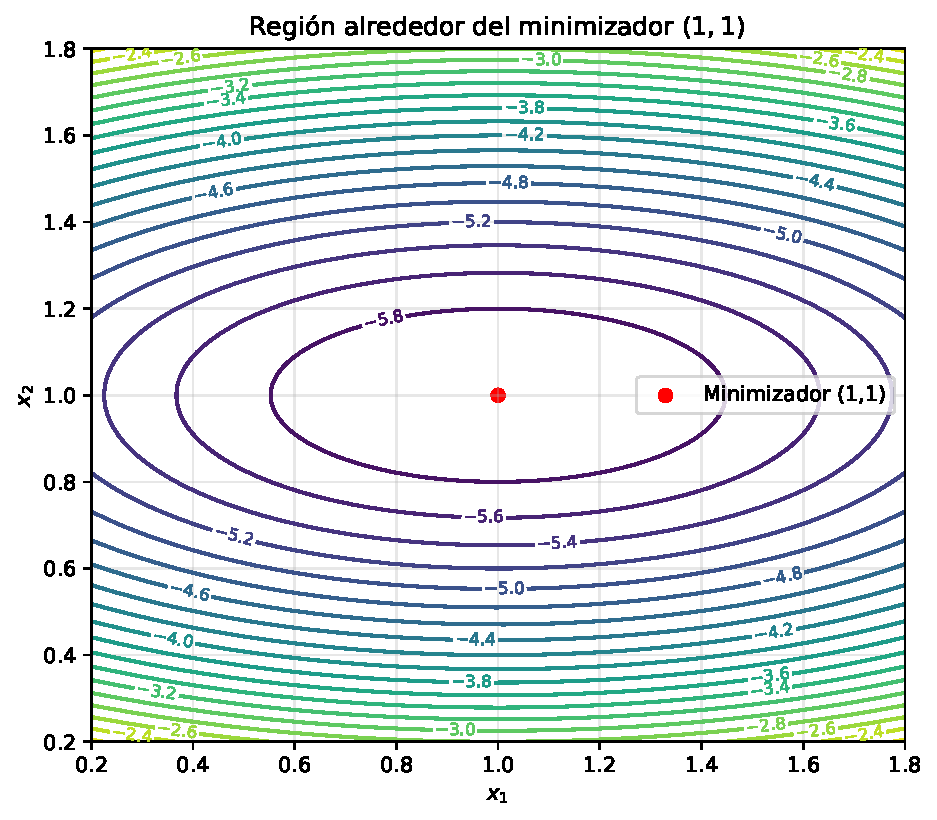
\includegraphics[keepaspectratio]{chapters/metodos_files/figure-pdf/cell-2-output-1.pdf}}

}

\caption{Visualización de la estructura geométrica de la función
cuadrática en un vecindario del minimizador global (1,1). Las elipses de
nivel reflejan la convexidad fuerte del modelo y la direccionalidad de
la curvatura asociada a la matriz Hessiana diagonal \(A\),
proporcionando una base geométrica para analizar el comportamiento local
de métodos iterativos como BFGS.}

\end{figure}%

Partimos de \(x_0 = (0, 0)^\top\) y elegimos \(H_0 = I\) como
aproximación inicial de la inversa del Hessiano. Utilizamos búsqueda
lineal exacta.

\textbf{Iteración \(k = 0\):}

\begin{itemize}
\tightlist
\item
  \(\nabla f(x_0) = A x_0 - b = (-2, -10)^\top\).
\item
  Dirección: \(p_0 = -H_0 \nabla f(x_0) = (2, 10)^\top\).
\item
  Paso óptimo: \[
  \alpha_0 = \frac{\nabla f(x_0)^\top p_0}{p_0^\top A p_0}
  = \frac{104}{1008} = \frac{13}{126} \approx 0.1032.
  \]
\item
  Nuevo punto: \[
  x_1 = x_0 + \alpha_0 p_0 = (0.2063, 1.0317)^\top.
  \]
\item
  Incrementos: \[
  s_0 = x_1 - x_0, \quad y_0 = \nabla f(x_1) - \nabla f(x_0) = A s_0.
  \]
\item
  Condición de curvatura: \(y_0^\top s_0 \approx 10.746 > 0\).
\item
  Actualización BFGS: \[
  H_1 \approx
  \begin{pmatrix} 0.503 & -0.004 \\ -0.004 & 0.100 \end{pmatrix},
  \] que aproxima bien a \(A^{-1} = \operatorname{diag}(0.5, 0.1)\).
\end{itemize}

\textbf{Iteración \(k = 1\):}

\begin{itemize}
\tightlist
\item
  \(\nabla f(x_1) = A x_1 - b \approx (-1.587, 0.317)^\top\).
\item
  Dirección: \(p_1 = -H_1 \nabla f(x_1) \approx (0.792, -0.032)^\top\).
\item
  Paso óptimo: \(\alpha_1 \approx 1.033\).
\item
  Nuevo punto: \(x_2 \approx (1.022, 0.999)^\top\), muy cercano a
  \(x^\star = (1,1)^\top\).
\end{itemize}

En solo dos iteraciones el algoritmo reduce el error residual en más de
un orden de magnitud, demostrando la \textbf{convergencia superlineal}
(ver Sección~\ref{sec-convergenciasuperlineal}) del método BFGS para
funciones cuadráticas. Este comportamiento se mantiene en problemas no
cuadráticos siempre que el condicionamiento sea razonable y la búsqueda
lineal sea suficientemente precisa.

\subsection{Familia Broyden y el método BFGS como caso
prototípico}\label{familia-broyden-y-el-muxe9todo-bfgs-como-caso-prototuxedpico}

La clase de métodos cuasi-Newton puede organizarse en torno a la
\textbf{familia de actualizaciones de Broyden}, un conjunto paramétrico
de fórmulas que preservan la ecuación secante y generan matrices
simétricas actualizadas a partir de la información de gradiente
acumulada. Esta familia engloba los métodos más relevantes en la
práctica, entre ellos el \textbf{BFGS}
(Broyden--Fletcher--Goldfarb--Shanno) y el \textbf{DFP}
(Davidon--Fletcher--Powell), y permite, como se expone en la Sección 6.3
de Nocedal y Wright (2006), analizar de forma unificada sus propiedades
de convergencia, estabilidad y eficiencia computacional.

Sea \(f : \mathbb{R}^n \to \mathbb{R}\) una función dos veces
continuamente diferenciable (ver Sección~\ref{sec-funcion_CD}). En cada
iteración \(k\), se dispone de los incrementos

\[
s_k := x_{k+1} - x_k, \quad y_k := \nabla f(x_{k+1}) - \nabla f(x_k),
\]

y se busca una matriz simétrica \(B_{k+1} \in \mathbb{R}^{n \times n}\)
que satisfaga la \textbf{ecuación secante}

\begin{equation}\phantomsection\label{eq-11}{
B_{k+1} s_k = y_k. 
}\end{equation}

La \textbf{familia de Broyden} se define como el conjunto de
actualizaciones

\begin{equation}\phantomsection\label{eq-broy}{
B_{k+1}(\phi_k) = B_k - \frac{B_k s_k s_k^\top B_k}{s_k^\top B_k s_k}
+ \frac{y_k y_k^\top}{y_k^\top s_k} + \phi_k\, v_k v_k^\top,
}\end{equation}

donde

\begin{equation}\phantomsection\label{eq-13}{
v_k = \left(\frac{y_k}{y_k^\top s_k} - \frac{B_k s_k}{s_k^\top B_k s_k}\right), 
}\end{equation}

y \(\phi_k \in \mathbb{R}\) es un parámetro que determina el miembro
particular de la familia.

La fórmula Ecuación~\ref{eq-broy} puede interpretarse como una
combinación convexa de dos actualizaciones extremas:

\begin{itemize}
\tightlist
\item
  \textbf{BFGS}: \(\phi_k = 0\),
\item
  \textbf{DFP}: \(\phi_k = 1\).
\end{itemize}

De hecho,

\begin{equation}\phantomsection\label{eq-14}{
B_{k+1}(\phi_k) = (1 - \phi_k) B_{k+1}^{\text{BFGS}} + \phi_k B_{k+1}^{\text{DFP}}. 
}\end{equation}

\subsubsection{Propiedades de la familia restringida de
Broyden}\label{propiedades-de-la-familia-restringida-de-broyden}

Una subclase especialmente relevante es la \textbf{familia restringida
de Broyden}, asociada a \(\phi_k \in [0,1]\). Bajo la \textbf{condición
de curvatura}

\begin{equation}\phantomsection\label{eq-15}{
y_k^\top s_k > 0, 
}\end{equation}

garantizada si la búsqueda lineal cumple las condiciones de Wolfe, todos
los miembros de esta subclase preservan la \textbf{definida positividad}
de \(B_k\), siempre que \(B_0\) sea simétrica definida positiva. Esta
propiedad asegura que la dirección de búsqueda

\begin{equation}\phantomsection\label{eq-16}{
p_k = -B_k^{-1} \nabla f(x_k)
}\end{equation}

sea de descenso. Además, si \(f\) es una función cuadrática fuertemente
convexa (ver Sección~\ref{sec-funcion_CD}), cualquier método de la
familia restringida de Broyden converge en a lo sumo \(n\) pasos,
generando direcciones conjugadas (ver Sección~\ref{sec-funcion_CD})
respecto al Hessiano exacto \(\nabla^2 f\) Dennis y Moré (1977), Sección
5.

\subsubsection{El método BFGS como caso
prototípico}\label{el-muxe9todo-bfgs-como-caso-prototuxedpico}

El método \textbf{BFGS} corresponde a \(\phi_k = 0\) en
Ecuación~\ref{eq-broy}. Su fórmula de actualización de la
\textbf{inversa del Hessiano aproximado} \(H_k = B_k^{-1}\) es

\begin{equation}\phantomsection\label{eq-17}{
H_{k+1} = (I - \rho_k s_k y_k^\top) H_k (I - \rho_k y_k s_k^\top) + \rho_k s_k s_k^\top,
\quad \rho_k = (y_k^\top s_k)^{-1}. 
}\end{equation}

Esta formulación evita la inversión explícita de matrices y facilita el
cálculo de la dirección de búsqueda:

\[
p_k = -H_k \nabla f(x_k).
\]

El método BFGS se distingue por:

\begin{itemize}
\tightlist
\item
  Su \textbf{invariancia afín}: el comportamiento es independiente de
  escalas y transformaciones lineales.
\item
  Su \textbf{propiedad de autocorrección} (\emph{self-scaling}): si
  \(H_k\) es una mala aproximación, la iteración corrige rápidamente la
  orientación de la matriz.
\item
  Su \textbf{convergencia superlineal} está garantizada bajo hipótesis
  estándar de suavidad, es decir, que \(f\) sea dos veces continuamente
  diferenciable (ver Sección~\ref{sec-funcion_CD}) y que su gradiente
  (o, equivalentemente, su Hessiano) sea Lipschitz continuo en una
  vecindad del minimizador, junto con el uso de una búsqueda lineal que
  satisfaga las condiciones de Wolfe, como se establece en Fletcher
  (1987), Sección 3.4.
\end{itemize}

\subsubsection{\texorpdfstring{Ejemplo ilustrativo: actualización BFGS
en
\(\mathbb{R}^2\)}{Ejemplo ilustrativo: actualización BFGS en \textbackslash mathbb\{R\}\^{}2}}\label{ejemplo-ilustrativo-actualizaciuxf3n-bfgs-en-mathbbr2}

Sea

\[
f(x) = \tfrac{1}{2} x^\top A x - b^\top x, \quad
A = \begin{pmatrix} 4 & 1 \\ 1 & 2 \end{pmatrix}, \quad
b = \begin{pmatrix} 1 \\ 1 \end{pmatrix}.
\]

El minimizador es
\(x^\star = A^{-1}b = (1/7, 3/7)^\top \approx (0.1429, 0.4286)^\top\).
Partimos de \(x_0 = (0,0)^\top\) y \(H_0 = I\).

\textbf{Iteración \(k = 0\):}

\begin{itemize}
\tightlist
\item
  \(\nabla f(x_0) = (-1, -1)^\top\).
\item
  \(p_0 = (1,1)^\top\).
\item
  \(\alpha_0 = \frac{2}{8} = 0.25\).
\item
  \(x_1 = (0.25, 0.25)^\top\).
\item
  \(\nabla f(x_1) = (0.25, -0.25)^\top\).
\item
  \(s_0 = (0.25, 0.25)^\top\), \(y_0 = (1.25, 0.75)^\top\).
\item
  \(y_0^\top s_0 = 0.5 > 0\), \(\rho_0 = 2\).
\item
  \(H_1 \approx \begin{pmatrix} 0.406 & -0.344 \\ -0.344 & 0.906 \end{pmatrix}\).
\end{itemize}

\textbf{Iteración \(k = 1\):}

\begin{itemize}
\tightlist
\item
  \(p_1 = -H_1 (0.25, -0.25)^\top \approx (-0.1875, 0.3125)^\top\).
\item
  \(\alpha_1 \approx 0.857\), \(x_2 \approx (0.089, 0.518)^\top\).
\end{itemize}

Tras dos iteraciones, \(\|x_2 - x^\star\| \approx 0.09\), y \(H_1\)
aproxima bien \(A^{-1}\), demostrando la capacidad del método para
capturar la geometría de segundo orden con pocas actualizaciones.

El método BFGS representa el \textbf{caso prototípico} dentro de la
familia de Broyden, al combinar eficiencia computacional, robustez
teórica y convergencia superlineal incluso en problemas moderadamente
mal condicionados.

\section{Extensión a dominios con restricciones tipo
caja}\label{extensiuxf3n-a-dominios-con-restricciones-tipo-caja}

En la práctica, muchos problemas de optimización imponen límites
naturales o estructurales sobre las variables de decisión, dando origen
a los denominados \textbf{problemas con restricciones tipo caja}. En
este contexto, las variables están acotadas por límites inferiores y
superiores que definen un dominio factible de la forma
\(\Omega = \{x \in \mathbb{R}^n : \ell_i \le x_i \le u_i\}\).

Estos problemas aparecen con frecuencia en aplicaciones de ingeniería,
finanzas y logística, donde ciertas magnitudes no pueden sobrepasar
intervalos físicamente admisibles. Extender los métodos de optimización
a dominios de este tipo requiere incorporar operadores de
\textbf{proyección ortogonal} que aseguren la factibilidad de cada
iteración sin comprometer la convergencia del algoritmo. La presente
sección desarrolla las propiedades analíticas de dicha proyección, que
constituye el núcleo geométrico de los métodos con restricciones tipo
caja.

\subsection{Proyección ortogonal sobre conjuntos de cotas: definición y
propiedades}\label{proyecciuxf3n-ortogonal-sobre-conjuntos-de-cotas-definiciuxf3n-y-propiedades}

En la optimización con restricciones tipo caja, el \textbf{conjunto
factible} se define como

\[
\Omega = \{x \in \mathbb{R}^n : \ell_i \le x_i \le u_i,\; i = 1,\dots,n\},
\]

donde
\(\ell = (\ell_1,\dots,\ell_n)^\top \in \mathbb{R}^n \cup \{-\infty\}^n\)
y \(u = (u_1,\dots,u_n)^\top \in \mathbb{R}^n \cup \{+\infty\}^n\)
satisfacen \(\ell_i < u_i\) para todo \(i\). Este conjunto es
\textbf{convexo, cerrado y no vacío}, lo que garantiza que la proyección
ortogonal de cualquier punto \(z \in \mathbb{R}^n\) sobre \(\Omega\)
está bien definida y es única.

\subsubsection{Proyección Ortogonal}\label{proyecciuxf3n-ortogonal}

La proyección ortogonal de \(z\) sobre \(\Omega\), denotada
\(P_\Omega(z)\), se define como la solución única del problema de
minimización

\begin{equation}\phantomsection\label{eq-18}{
P_\Omega(z) = \arg\min_{x \in \Omega} \tfrac{1}{2}\|x - z\|^2. 
}\end{equation}

Dado que \(\Omega\) es un producto cartesiano de intervalos cerrados, la
proyección se \textbf{descompone coordenada a coordenada}:

\begin{equation}\phantomsection\label{eq-19}{
[P_\Omega(z)]_i = \min\{u_i,\, \max\{\ell_i,\, z_i\}\}, \quad i = 1,\dots,n. 
}\end{equation}

Esta expresión corresponde a la llamada \emph{función de recorte}
(\emph{clipping function}), que restringe cada componente de \(z\) al
intervalo factible \([\ell_i,u_i]\).

\subsubsection{Propiedades
fundamentales}\label{propiedades-fundamentales}

\begin{enumerate}
\def\labelenumi{\arabic{enumi}.}
\item
  \textbf{No expansividad}

  \begin{equation}\phantomsection\label{eq-20}{
  \|P_\Omega(z) - P_\Omega(w)\| \le \|z - w\|, \quad \forall z,w \in \mathbb{R}^n.
  }\end{equation}

  Por tanto, \(P_\Omega\) es una aplicación \textbf{Lipschitz continua
  (ver Sección~\ref{sec-funcion_CD}) con constante 1}, lo que implica
  estabilidad numérica.
\item
  \textbf{Caracterización variacional}

  Un punto \(x^\star \in \Omega\) satisface \(x^\star = P_\Omega(z)\),
  si y solo si,

  \begin{equation}\phantomsection\label{eq-21}{
  (z - x^\star)^\top (x - x^\star) \le 0, \quad \forall x \in \Omega.
  }\end{equation}

  Geométricamente, esto significa que el vector residual \(z - x^\star\)
  forma un ángulo obtuso con cualquier dirección factible desde
  \(x^\star\).
\item
  \textbf{Condiciones de complementariedad (KKT)}

  Para cada \(i\) se cumple

  \begin{equation}\phantomsection\label{eq-22}{
  \begin{cases}
  x_i = \ell_i &\Rightarrow z_i \le \ell_i,\\[4pt]
  x_i = u_i &\Rightarrow z_i \ge u_i,\\[4pt]
  \ell_i < x_i < u_i &\Rightarrow z_i = x_i,
  \end{cases}
  }\end{equation}

  que equivalen a las condiciones de optimalidad de primer orden del
  problema cuadrático (Ecuación~\ref{eq-18}).
\end{enumerate}

\subsubsection{\texorpdfstring{Ejemplo: proyección en
\(\mathbb{R}^3\)}{Ejemplo: proyección en \textbackslash mathbb\{R\}\^{}3}}\label{ejemplo-proyecciuxf3n-en-mathbbr3}

Sea

\[
\Omega = \{x \in \mathbb{R}^3 : 1 \le x_1 \le 3,\; x_2 \le 2,\; x_3 \ge 0\},
\quad z = (0.5,\, 2.5,\, -1.2)^\top.
\]

Aplicando Ecuación~\ref{eq-19} coordenada a coordenada:

\begin{itemize}
\tightlist
\item
  \(x_1^\star = \min\{3, \max\{1, 0.5\}\} = 1\),
\item
  \(x_2^\star = \min\{2, \max\{-\infty, 2.5\}\} = 2\),
\item
  \(x_3^\star = \min\{+\infty, \max\{0, -1.2\}\} = 0\).
\end{itemize}

Por tanto,

\[
P_\Omega(z) = (1,\, 2,\, 0)^\top.
\]

Comprobamos la caracterización variacional:

\[
(z - x^\star)^\top (x - x^\star)
= (-0.5,\, 0.5,\, -1.2)^\top \cdot (x_1-1,\, x_2-2,\, x_3-0).
\]

Dado que \(x_1 \ge 1\), \(x_2 \le 2\), \(x_3 \ge 0\), cada término
parcial es no positivo, y la suma total \(\le 0\).\\
Asimismo, las condiciones Ecuación~\ref{eq-22} se satisfacen coordenada
a coordenada: \(x_1^\star=1\) con \(z_1=0.5\le1\), \(x_2^\star=2\) con
\(z_2=2.5\ge2\), y \(x_3^\star=0\) con \(z_3=-1.2\le0\).

Este ejemplo ilustra cómo la proyección actúa localmente sobre cada
componente, garantizando factibilidad sin resolver sistemas lineales. Su
simplicidad y propiedades de estabilidad hacen que el operador
\(P_\Omega\) sea esencial en algoritmos de optimización a gran escala,
como el método \textbf{L-BFGS-B}, en el cual se aplica en cada iteración
para mantener las variables dentro de los límites definidos.

\subsection{El algoritmo L-BFGS-B: formulación y justificación
estructural}\label{el-algoritmo-l-bfgs-b-formulaciuxf3n-y-justificaciuxf3n-estructural}

El algoritmo \textbf{L-BFGS-B} (\emph{Limited-memory BFGS with Bounds})
extiende el método cuasi-Newton BFGS al caso de \textbf{restricciones
tipo caja}, es decir, dominios de la forma

\[
\Omega = \{x \in \mathbb{R}^n : \ell \le x \le u\},
\]

donde las desigualdades son componente a componente y
\(\ell, u \in \mathbb{R}^n \cup \{\pm\infty\}^n\) con
\(\ell_i < u_i\).\\
El método integra tres ideas fundamentales:

\begin{enumerate}
\def\labelenumi{\arabic{enumi}.}
\tightlist
\item
  \textbf{Aproximación cuasi-Newton de memoria limitada}, evitando el
  almacenamiento completo de matrices densas;
\item
  \textbf{Proyección ortogonal} sobre \(\Omega\) para mantener
  factibilidad;
\item
  \textbf{Retención parcial de información de curvatura}, conservando
  sólo las \(m\) parejas más recientes \((s_i, y_i)\).
\end{enumerate}

\subsubsection{Formulación del
algoritmo}\label{formulaciuxf3n-del-algoritmo}

Dado un punto inicial \(x_0 \in \Omega\), el esquema iterativo se
expresa como

\begin{equation}\phantomsection\label{eq-23}{
x_{k+1} = P_\Omega\big(x_k - \alpha_k H_k \nabla f(x_k)\big),
}\end{equation}

donde \(\alpha_k > 0\) satisface las condiciones de Wolfe y \(H_k\) es
la aproximación de memoria limitada al inverso del Hessiano, construida
mediante las \(m\) actualizaciones más recientes:

\[
s_i = x_{i+1} - x_i, \qquad
y_i = \nabla f(x_{i+1}) - \nabla f(x_i), \quad i = k-m,\dots,k-1,
\]

con \(y_i^\top s_i > 0\) (condición de curvatura).\\
La proyección \(P_\Omega\) se calcula coordenada a coordenada como

\begin{equation}\phantomsection\label{eq-24}{
[P_\Omega(z)]_i = \min\{u_i, \max\{\ell_i, z_i\}\}, \quad i=1,\dots,n. 
}\end{equation}

El producto \(H_k \nabla f(x_k)\) se obtiene por la \textbf{recursión de
dos bucles}, iniciada con \(H_k^{(0)} = \gamma_k I\), donde

\begin{equation}\phantomsection\label{eq-25}{
\gamma_k = \frac{s_{k-1}^\top y_{k-1}}{y_{k-1}^\top y_{k-1}}. 
}\end{equation}

Este escalamiento mejora la estabilidad numérica y la aceptación de
pasos unitarios.

\subsubsection{Justificación
estructural}\label{justificaciuxf3n-estructural}

El esquema Ecuación~\ref{eq-23} garantiza factibilidad a cada iteración
mediante la proyección \(P_\Omega\).\\
Definiendo el conjunto de índices activos

\[
\mathcal{A}_k = \{i : x_{k,i} = \ell_i \text{ o } x_{k,i} = u_i\},
\]

el método se comporta localmente como BFGS en los índices inactivos
(\(i \notin \mathcal{A}_k\)) y mantiene las componentes activas en las
cotas.\\
De este modo, la actualización proyectada puede interpretarse como

\[
x_{k+1} = \operatorname{Proj}_\Omega\big(x_k - \alpha_k \nabla^2 f(x_k)^{-1} \nabla f(x_k)\big),
\]

con \(\nabla^2 f(x_k)^{-1}\) sustituido por la aproximación limitada
\(H_k\).\\
Esta interpretación explica por qué L-BFGS-B conserva tanto la
factibilidad como las propiedades de descenso y la convergencia
superlineal del BFGS original.

En términos computacionales, el método BFGS requiere
\(\mathcal{O}(n^2)\) unidades de memoria. Esto se debe a que, en cada
iteración, el algoritmo mantiene una representación explícita de una
matriz simétrica \(H_k \in \mathbb{R}^{n \times n}\) que aproxima la
inversa del Hessiano de la función objetivo. El almacenamiento de dicha
matriz implica retener el orden de \(n^2\) números reales en memoria
principal, lo cual constituye un costo cuadrático en la dimensión del
problema. Este requisito es inherente a la formulación clásica del
método, ya que tanto la actualización de \(H_k\) mediante la fórmula
cuasi-Newton como el cálculo de la dirección de búsqueda
\(p_k = -H_k \nabla f(x_k)\) dependen de acceso directo a todos los
elementos de la matriz. En problemas de gran escala, donde \(n\) puede
alcanzar órdenes de magnitud de \(10^5\) o más, este costo se vuelve
prohibitivo desde el punto de vista práctico. En contraste, el algoritmo
L-BFGS-B evita el almacenamiento explícito de \(H_k\) y solo retiene los
últimos \(m\) pares de vectores \((s_k, y_k)\), lo que reduce el
requerimiento de memoria a \(\mathcal{O}(mn)\), con \(m \ll n\)
(típicamente \(3 \leq m \leq 20\)).

\subsubsection{Ejemplo: minimización cuadrática con restricciones tipo
caja}\label{ejemplo-minimizaciuxf3n-cuadruxe1tica-con-restricciones-tipo-caja}

Considérese

\[
\min_{x \in \mathbb{R}^2} f(x) = (x_1 - 2)^2 + (x_2 - 1)^2
\quad \text{sujeto a} \quad 1 \le x_1 \le 3, \; x_2 \ge 0.
\]

El minimizador irrestricto \(x^\star = (2,1)^\top\) pertenece a
\(\Omega\), por lo que coincide con el minimizador restringido.\\
Con \(m=1\) y \(x_0=(1,0)^\top\), el procedimiento es:

\textbf{Iteración 0}

\(\nabla f(x_0)=(-2,-2)^\top\), \(H_0=I\), \(d_0=(2,2)^\top\).\\
Con \(\alpha_0=1\), se obtiene \(\tilde{x}_1=(3,2)^\top\) y
\(x_1=P_\Omega(\tilde{x}_1)=(3,2)^\top\).\\
\(\nabla f(x_1)=(2,2)^\top\), \(s_0=(2,2)^\top\), \(y_0=(4,4)^\top\).

\textbf{Iteración 1}

\(\gamma_1=\tfrac{s_0^\top y_0}{y_0^\top y_0}=0.5\),\\
\(H_1^{(0)}=0.5I\).\\
Aplicando la recursión de dos bucles:

\(q=\nabla f(x_1)\), \(\alpha_0=0.5\), \(q=q-0.5y_0=(0,0)^\top\),\\
\(r=H_1^{(0)}q=(0,0)^\top\),\\
\(r=r+s_0(\alpha_0-\tfrac{y_0^\top r}{y_0^\top s_0})=(1,1)^\top\).\\
Dirección \(d_1=-r=(-1,-1)^\top\).\\
Con \(\alpha_1=1\), \(\tilde{x}_2=(2,1)^\top\),
\(x_2=P_\Omega(\tilde{x}_2)=(2,1)^\top\).

El método converge en dos iteraciones, demostrando que la estructura de
memoria limitada y la proyección garantizan simultáneamente
\textbf{eficiencia y factibilidad}.

La formulación L-BFGS-B preserva las propiedades de convergencia global
del BFGS bajo las hipótesis de suavidad y curvatura positiva. Para más
detalles Byrd et~al. (1995); Zhu et~al. (1997), y constituye uno de los
métodos estándar para problemas de gran escala con restricciones tipo
caja.

\subsection{Condiciones de optimalidad bajo cotas: KKT para problemas
con restricciones tipo caja}\label{sec-kkt_caja}

Tras haber introducido la formulación proyectada del algoritmo L-BFGS-B,
resulta necesario caracterizar formalmente las condiciones de
optimalidad que dicho método busca satisfacer. En particular, cuando el
dominio está delimitado por cotas inferiores y superiores, las
condiciones de Karush--Kuhn--Tucker (KKT) Sección~\ref{sec-kkt}
adquieren una estructura particularmente simple y separable por
coordenadas. Esta sección desarrolla esa caracterización, que constituye
el fundamento teórico de la convergencia de los métodos con
restricciones tipo caja.

Consideremos el problema de optimización

\begin{equation}\phantomsection\label{eq-26}{
\min_{x \in \mathbb{R}^n} f(x)
\quad \text{sujeto a} \quad
\ell \le x \le u,
}\end{equation}

donde \(f: \mathbb{R}^n \to \mathbb{R}\) es continuamente diferenciable
(ver Sección~\ref{sec-funcion_CD}) en un conjunto abierto que contiene
al conjunto factible

\[
\Omega = \{x \in \mathbb{R}^n : \ell_i \le x_i \le u_i,\; i=1,\dots,n\},
\]

con \(\ell_i < u_i\) para todo \(i\). Este problema constituye un caso
particular de programación no lineal con restricciones de desigualdad
simples.

\subsubsection{Condiciones de Karush--Kuhn--Tucker
(KKT)}\label{condiciones-de-karushkuhntucker-kkt}

Reescribiendo las restricciones como desigualdades estándar,

\begin{equation}\phantomsection\label{eq-27}{
c_i^{\ell}(x) := \ell_i - x_i \le 0, \qquad
c_i^{u}(x) := x_i - u_i \le 0, \quad i = 1,\dots,n,
}\end{equation}

y suponiendo que se cumple la condición de calificación de
Mangasarian--Fromovitz (MFQC), las \textbf{condiciones necesarias de
Karush--Kuhn--Tucker} establecen que si \(x^\star \in \Omega\) es un
minimizador local, existen multiplicadores de Lagrange
\(\lambda^\ell, \lambda^u \in \mathbb{R}^n\) tales que

\begin{equation}\phantomsection\label{eq-kkt-a}{
\nabla f(x^\star) - \lambda^\ell + \lambda^u = 0.
}\end{equation}

\begin{equation}\phantomsection\label{eq-kkt-b}{
\lambda_i^\ell \ge 0,\quad \lambda_i^u \ge 0.
}\end{equation}

\begin{equation}\phantomsection\label{eq-kkt-c}{
\lambda_i^\ell (x_i^\star - \ell_i) = 0.
}\end{equation}

\begin{equation}\phantomsection\label{eq-kkt-d}{
\lambda_i^u (u_i - x_i^\star) = 0.
}\end{equation}

para todo \(i = 1,\dots,n\).\\
Las ecuaciones Ecuación~\ref{eq-kkt-c}--Ecuación~\ref{eq-kkt-d} expresan
la \textbf{complementariedad} entre los multiplicadores y las
restricciones activas.

\subsubsection{Forma equivalente sin
multiplicadores}\label{forma-equivalente-sin-multiplicadores}

Eliminando \(\lambda^\ell\) y \(\lambda^u\), las condiciones KKT pueden
escribirse componente a componente como

\begin{equation}\phantomsection\label{eq-29}{
\forall i = 1,\dots,n:
\quad
\begin{cases}
\nabla_i f(x^\star) = 0, & \text{si } \ell_i < x_i^\star < u_i,\\[4pt]
\nabla_i f(x^\star) \ge 0, & \text{si } x_i^\star = \ell_i,\\[4pt]
\nabla_i f(x^\star) \le 0, & \text{si } x_i^\star = u_i,
\end{cases}
}\end{equation}

donde las desigualdades se interpretan componente a componente.\\
Geométricamente, esto significa que el gradiente proyectado sobre el
\textbf{cono tangente} de \(\Omega\) en \(x^\star\) es nulo.

Una formulación alternativa, útil en algoritmos numéricos, es la
\textbf{condición de estacionariedad proyectada}:

\begin{equation}\phantomsection\label{eq-30}{
\nabla_\Omega f(x^\star)
:= P_\Omega\big(x^\star - \nabla f(x^\star)\big) - x^\star
= 0.
}\end{equation}

La igualdad Ecuación~\ref{eq-30} es \textbf{equivalente} a las
condiciones KKT cuando \(f\) es convexa, y constituye una
\textbf{condición necesaria} de optimalidad en el caso no convexo. En la
práctica, se emplea como criterio de convergencia en algoritmos
proyectados como L-BFGS-B.

\subsubsection{Ejemplo: verificación explícita de
KKT}\label{ejemplo-verificaciuxf3n-expluxedcita-de-kkt}

Sea

\begin{equation}\phantomsection\label{eq-31}{
\min_{x \in \mathbb{R}^2} f(x) = (x_1 - 1)^2 + (x_2 - 2)^2,
\quad
\text{sujeto a } 1 \le x_1 \le 3,\; x_2 \ge 0.
}\end{equation}

El gradiente es \(\nabla f(x) = (2(x_1 - 1),\, 2(x_2 - 2))^\top\).

\textbf{Paso 1. Identificación del candidato.}\\
El minimizador irrestricto \((1,2)^\top\) pertenece a \(\Omega\), por lo
tanto \(x^\star = (1,2)^\top\) es candidato a solución óptima.

\textbf{Paso 2. Verificación de Ecuación~\ref{eq-29}.}\\
- \(x_1^\star = \ell_1 = 1 \Rightarrow \nabla_1 f(x^\star) = 0 \ge 0\)
✓\\
- \(\ell_2 < x_2^\star < +\infty \Rightarrow \nabla_2 f(x^\star) = 0\) ✓

\textbf{Paso 3. Multiplicadores KKT.}\\
De Ecuación~\ref{eq-kkt-a}, \[
\nabla f(x^\star) - \lambda^\ell + \lambda^u = 0
\Rightarrow \lambda^\ell = \lambda^u = 0.
\]

\textbf{Paso 4. Estacionariedad proyectada.}\\
\[
x^\star - \nabla f(x^\star) = (1,2),\quad
P_\Omega(1,2) = (1,2),
\quad \Rightarrow \nabla_\Omega f(x^\star) = 0.
\]

Así, \(x^\star\) satisface todas las condiciones de Karush--Kuhn--Tucker
y es el minimizador global.

Este análisis demuestra que las condiciones KKT para restricciones tipo
caja poseen una estructura \textbf{desacoplada y local}, lo que permite
su implementación eficiente en métodos de gran escala. En particular, la
condición proyectada Ecuación~\ref{eq-30} constituye la base teórica de
los algoritmos de proyección iterativa, incluyendo el método L-BFGS-B,
cuya convergencia global se verifica precisamente mediante la nulidad
asintótica de \(\nabla_\Omega f(x_k)\).

\section{Convergencia del método
L-BFGS-B}\label{convergencia-del-muxe9todo-l-bfgs-b}

\subsection{Hipótesis de regularidad: Lipschitz-continuidad del
gradiente y compacidad del
dominio}\label{hipuxf3tesis-de-regularidad-lipschitz-continuidad-del-gradiente-y-compacidad-del-dominio}

El análisis de convergencia global del algoritmo \textbf{L-BFGS-B}
requiere hipótesis estructurales sobre la función objetivo
\(f : \mathbb{R}^n \to \mathbb{R}\) y sobre el conjunto factible
\(\Omega \subset \mathbb{R}^n\). Estas condiciones garantizan la
existencia de minimizadores, la acotación de las iteraciones y la
controlabilidad del gradiente, elementos esenciales para asegurar tanto
la \textbf{bien definición del algoritmo} como su \textbf{convergencia
hacia puntos estacionarios}.

\subsubsection{Hipótesis
fundamentales}\label{hipuxf3tesis-fundamentales}

Sea \[
\Omega = \{ x \in \mathbb{R}^n : \ell \le x \le u \},
\]

con \(\ell, u \in \mathbb{R}^n \cup \{\pm\infty\}^n\) y \(\ell_i < u_i\)
para todo \(i\). Supondremos que \(f\) satisface las siguientes
condiciones:

\begin{quote}
\textbf{(H1) Diferenciabilidad y Lipschitz-continuidad del gradiente.}\\
La función \(f\) es continuamente diferenciable (ver
Sección~\ref{sec-funcion_CD}) en un conjunto abierto que contiene a
\(\Omega\), y su gradiente \(\nabla f\) es \textbf{Lipschitz continuo}
en \(\Omega\); es decir, existe una constante \(L > 0\) tal que\\
\begin{equation}\phantomsection\label{eq-37}{
\|\nabla f(x) - \nabla f(y)\| \le L \|x - y\|, \quad \forall x, y \in \Omega.
}\end{equation}
\end{quote}

\begin{quote}
\textbf{(H2) Compacidad del conjunto de nivel inicial.}\\
Dado un punto inicial \(x_0 \in \Omega\), el conjunto de nivel
asociado\\
\begin{equation}\phantomsection\label{eq-38}{
\mathcal{L} := \{ x \in \Omega : f(x) \le f(x_0) \} 
}\end{equation} es \textbf{no vacío, cerrado y acotado}, y por tanto
\textbf{compacto}.
\end{quote}

La hipótesis (H1) implica que el gradiente no cambia bruscamente, lo que
permite controlar los pasos del algoritmo mediante la cota superior
\(L\). Equivalentemente, la desigualdad de suavidad se cumple:
\begin{equation}\phantomsection\label{eq-hipotesis}{
f(y) \le f(x) + \nabla f(x)^\top (y-x) + \tfrac{L}{2}\|y-x\|^2, \quad \forall x, y \in \Omega. 
}\end{equation} Esta relación garantiza que las búsquedas lineales que
satisfacen las \textbf{condiciones de Wolfe} producen pasos
uniformemente acotados y no degenerados.

La hipótesis (H2), por su parte, asegura que las iteraciones \(\{x_k\}\)
permanecen en un subconjunto \textbf{compacto y factible} de \(\Omega\).
Esto permite aplicar resultados de convergencia por subsucesión y
garantiza que las secuencias de gradientes y valores de función no
divergen.

\subsubsection{Consecuencias teóricas}\label{consecuencias-teuxf3ricas}

Bajo las hipótesis (H1) y (H2), la sucesión \(\{x_k\}\) generada por
L-BFGS-B con una búsqueda lineal que cumple las condiciones de Wolfe
posee las siguientes propiedades:

\begin{enumerate}
\def\labelenumi{\arabic{enumi}.}
\item
  \textbf{Existencia de puntos límite.}\\
  Toda subsucesión de \(\{x_k\}\) posee una subsucesión convergente cuyo
  límite pertenece a \(\mathcal{L} \subset \Omega\).
\item
  \textbf{Condición de curvatura.}\\
  Las parejas de actualización\\
  \[
  s_k = x_{k+1} - x_k, \quad y_k = \nabla f(x_{k+1}) - \nabla f(x_k),
  \] satisfacen \(y_k^\top s_k > 0\) siempre que se cumplan las
  condiciones de Wolfe, lo que garantiza que las aproximaciones
  cuasi-Newton sean definidas positivas (Byrd et al., 1995).
\item
  \textbf{Acotación de los operadores de memoria limitada.}\\
  La recursión de dos bucles empleada en L-BFGS-B mantiene direcciones
  de búsqueda acotadas y de descenso, gracias a la compacidad de
  \(\mathcal{L}\) y a la positividad de los escalares
  \(\rho_k = (y_k^\top s_k)^{-1}\).
\end{enumerate}

\subsubsection{Teorema de convergencia global (versión
esquemática)}\label{teorema-de-convergencia-global-versiuxf3n-esquemuxe1tica}

\textbf{Teorema.}\\
Supóngase que \(f\) satisface (H1) y (H2), y que la búsqueda lineal
cumple las condiciones de Wolfe. Si las actualizaciones de memoria
limitada satisfacen \(y_k^\top s_k > 0\) o son rechazadas en caso
contrario (salvaguarda numérica), entonces la sucesión \(\{x_k\}\)
generada por L-BFGS-B verifica
\begin{equation}\phantomsection\label{eq-40}{
\liminf_{k \to \infty} \|\nabla_\Omega f(x_k)\| = 0, 
}\end{equation} donde el \textbf{gradiente proyectado} se define como
\begin{equation}\phantomsection\label{eq-41}{
\nabla_\Omega f(x) := P_\Omega(x - \nabla f(x)) - x. 
}\end{equation}

\textbf{Bosquejo de prueba.}\\
De (H2) se sigue que \(\{x_k\} \subset \mathcal{L}\) es acotada, por lo
que posee subsucesiones convergentes. La desigualdad
Ecuación~\ref{eq-hipotesis} y las condiciones de Wolfe garantizan un
descenso suficiente de \(f\). La condición de curvatura
\(y_k^\top s_k > 0\) asegura que las matrices \(H_k\) permanecen
definidas positivas y acotadas (Nocedal y Wright (2006), Teorema 3.2 y
Sección 6.1). Por tanto, todo punto límite \(\bar{x}\) de la sucesión
satisface la condición de estacionariedad proyectada
\(\nabla_\Omega f(\bar{x}) = 0\) (Byrd et~al. (1995), Teorema 4.1).

\subsubsection{Ejemplo de verificación de las
hipótesis}\label{ejemplo-de-verificaciuxf3n-de-las-hipuxf3tesis}

Consideremos el problema \begin{equation}\phantomsection\label{eq-42}{
\min_{x \in \mathbb{R}^2} f(x) = x_1^4 + x_2^2
\quad \text{sujeto a } 0 \le x_1 \le 2,\; -1 \le x_2 \le 1.
}\end{equation}

\textbf{Paso 1. Verificación de (H1).}\\
El gradiente es \[
\nabla f(x) = (4x_1^3, 2x_2)^\top, \quad
\nabla^2 f(x) = \begin{pmatrix} 12x_1^2 & 0 \\ 0 & 2 \end{pmatrix}.
\]

En \(\Omega = [0,2] \times [-1,1]\), \[
\|\nabla^2 f(x)\|_2 = \max\{12x_1^2, 2\} \le 48.
\] Por tanto, \(L = 48\) es una constante de Lipschitz para \(\nabla f\)
en \(\Omega\), y (H1) se cumple.

\textbf{Paso 2. Verificación de (H2).}\\
Sea \(x_0 = (2,1)^\top \in \Omega\). Entonces \[
f(x_0) = 2^4 + 1^2 = 17, \quad
\mathcal{L} = \{ x \in \Omega : x_1^4 + x_2^2 \le 17 \}.
\] Dado que \(\Omega\) es compacto y \(\mathcal{L} \subset \Omega\), el
conjunto de nivel es cerrado, acotado y no vacío (pues
\(x^\star = (0,0)^\top \in \mathcal{L}\)). Así, (H2) también se
satisface.

\textbf{Paso 3. Implicaciones para L-BFGS-B.}\\
Bajo estas condiciones, la sucesión \(\{x_k\}\) generada por L-BFGS-B
permanece en \(\mathcal{L}\), el gradiente es Lipschitz con constante
\(L = 48\), y las parejas \((s_k, y_k)\) satisfacen
\(y_k^\top s_k > 0\). Por tanto, el algoritmo produce direcciones de
descenso bien definidas, y los límites de las iteraciones satisfacen las
condiciones de Karush--Kuhn--Tucker bajo restricciones tipo caja.

En síntesis, las hipótesis (H1) y (H2) proporcionan el \textbf{marco
teórico mínimo} para garantizar la convergencia global del método
L-BFGS-B. Estas condiciones, verificables en la práctica, sustentan la
robustez del algoritmo en problemas suaves y acotados típicos de la
optimización aplicada.

\subsection{Teorema de convergencia global: límite de puntos
estacionarios que satisfacen KKT}\label{sec-convregencia_global}

El algoritmo \textbf{L-BFGS-B} está diseñado para resolver problemas de
optimización no lineal con restricciones tipo caja de la forma

\begin{equation}\phantomsection\label{eq-teo_con}{
\min_{x \in \mathbb{R}^n} f(x)
\quad \text{sujeto a} \quad \ell \le x \le u. 
}\end{equation}

Aquí, \(f : \mathbb{R}^n \to \mathbb{R}\) es continuamente diferenciable
(ver Sección~\ref{sec-funcion_CD}), y el conjunto factible

\[
\Omega = \{x \in \mathbb{R}^n : \ell \le x \le u\}
\]

es cerrado, convexo y no vacío.

El \textbf{resultado fundamental de convergencia global}, Byrd et~al.
(1995), establece que, bajo hipótesis estándar de regularidad y
condiciones adecuadas de búsqueda lineal, la sucesión generada por el
algoritmo posee puntos límite que satisfacen las \textbf{condiciones
necesarias de optimalidad de Karush--Kuhn--Tucker (KKT)}. Dicho de otra
forma, el algoritmo converge, en el sentido de subsecuencias, hacia el
conjunto de puntos estacionarios proyectados.

\subsubsection{Teorema de convergencia
global}\label{sec-teorema_convergencia}

\begin{quote}
\textbf{Teorema 6.2 (Convergencia global de L-BFGS-B).}\\
Sea \(f : \mathbb{R}^n \to \mathbb{R}\) una función continuamente
diferenciable que satisface:

\begin{enumerate}
\def\labelenumi{\arabic{enumi}.}
\tightlist
\item
  \(\nabla f\) es \textbf{Lipschitz continuo} en \(\Omega\); existe
  \(L > 0\) tal que\\
  \begin{equation}\phantomsection\label{eq-61}{
  \|\nabla f(x) - \nabla f(y)\| \le L \|x - y\|, \quad \forall x, y \in \Omega;
  }\end{equation}
\item
  El conjunto de nivel inicial\\
  \begin{equation}\phantomsection\label{eq-62}{
  \mathcal{L} := \{x \in \Omega : f(x) \le f(x_0)\} 
  }\end{equation} es \textbf{compacto}.
\end{enumerate}

Supóngase que la sucesión \(\{x_k\} \subset \Omega\) se genera mediante
el algoritmo L-BFGS-B con direcciones de búsqueda
\begin{equation}\phantomsection\label{eq-63}{
d_k = P_\Omega(x_k - H_k \nabla f(x_k)) - x_k, 
}\end{equation} donde \(H_k\) es la aproximación inversa del Hessiano
obtenida mediante la recursión de dos bucles con memoria limitada \(m\),
y que las longitudes de paso \(\alpha_k > 0\) satisfacen las
\textbf{condiciones de Wolfe}:
\begin{equation}\phantomsection\label{eq-64}{
\begin{aligned}
f(x_k + \alpha_k d_k) &\le f(x_k) + c_1 \alpha_k \nabla f(x_k)^\top d_k, \\
\nabla f(x_k + \alpha_k d_k)^\top d_k &\ge c_2 \nabla f(x_k)^\top d_k,
\end{aligned} 
}\end{equation} con \(0 < c_1 < c_2 < 1\).

Entonces, la sucesión \(\{x_k\}\) verifica:
\begin{equation}\phantomsection\label{eq-liminf}{
\liminf_{k \to \infty} \|\nabla_\Omega f(x_k)\| = 0,
}\end{equation} donde \begin{equation}\phantomsection\label{eq-66}{
\nabla_\Omega f(x) := P_\Omega(x - \nabla f(x)) - x 
}\end{equation} es el \textbf{gradiente proyectado}.\\
En consecuencia, toda subsucesión convergente de \(\{x_k\}\) converge a
un punto \(x^\star \in \Omega\) que satisface las \textbf{condiciones
KKT} del problema Ecuación~\ref{eq-teo_con}.
\end{quote}

\subsubsection{Bosquejo de la
demostración}\label{bosquejo-de-la-demostraciuxf3n}

\begin{enumerate}
\def\labelenumi{\arabic{enumi}.}
\item
  \textbf{Acotación de la sucesión.}\\
  Por compacidad de \(\mathcal{L}\), las iteraciones
  \(\{x_k\} \subset \mathcal{L}\) son acotadas, y existe una subsucesión
  convergente \(x_{k_j} \to x^\star \in \mathcal{L}\).
\item
  \textbf{Positividad de la curvatura.}\\
  Bajo las condiciones de Wolfe, las diferencias \(s_k = x_{k+1} - x_k\)
  y \(y_k = \nabla f(x_{k+1}) - \nabla f(x_k)\) satisfacen
  \begin{equation}\phantomsection\label{eq-67}{
  y_k^\top s_k \ge (1 - c_2)\|\nabla f(x_k)\|^2 \alpha_k > 0, 
  }\end{equation} asegurando que las actualizaciones L-BFGS mantengan
  \(H_k \succ 0\).
\item
  \textbf{Dirección de descenso.}\\
  La proyección garantiza que
  \begin{equation}\phantomsection\label{eq-68}{
  \nabla f(x_k)^\top d_k \le -\|d_k\|^2, 
  }\end{equation} es decir, \(d_k\) es una dirección de descenso o nula
  solo en puntos estacionarios.
\item
  \textbf{Aplicación del lema de Zoutendijk en problemas restringidos.}

  El lema de Zoutendijk original (Zoutendijk (1970), p.~40) se formuló
  para problemas sin restricciones, pero admite una extensión natural al
  caso de minimización sobre un conjunto convexo cerrado
  \(\Omega \subset \mathbb{R}^n\) (Nocedal y Wright (2006), Lema 12.1,
  p.~333). Bajo las hipótesis del teorema, en particular, que \(f\) es
  continuamente diferenciable (ver Sección~\ref{sec-funcion_CD}) con
  gradiente Lipschitz en un conjunto de nivel compacto, y que los pasos
  \(\alpha_k\) satisfacen las condiciones de Wolfe, la sucesión generada
  por un método de descenso proyectado verifica
  \begin{equation}\phantomsection\label{eq-wol}{
  \sum_{k=0}^\infty \frac{(\nabla f(x_k)^\top d_k)^2}{\|d_k\|^2} < \infty. 
  }\end{equation}

  En el caso del gradiente proyectado, la dirección de búsqueda se
  define como
  \(d_k = P_\Omega(x_k - \nabla f(x_k)) - x_k = \nabla_\Omega f(x_k)\).
  Una propiedad fundamental de la proyección ortogonal sobre un conjunto
  convexo es que satisface la desigualdad variacional \[
  (x_k - \nabla f(x_k) - (x_k + d_k))^\top (x - (x_k + d_k)) \le 0, \quad \forall x \in \Omega,
  \] la cual implica, en particular, que
  \begin{equation}\phantomsection\label{eq-69}{
  \nabla f(x_k)^\top d_k = -\|d_k\|^2. 
  }\end{equation} Sustituyendo en Ecuación~\ref{eq-wol}, obtenemos \[
  \sum_{k=0}^\infty \|d_k\|^2 < \infty.
  \] Esta serie convergente implica que \(\|d_k\| \to 0\) cuando
  \(k \to \infty\). Dado que \(d_k = \nabla_\Omega f(x_k)\), se concluye
  que \[
  \lim_{k \to \infty} \|\nabla_\Omega f(x_k)\| = 0,
  \] lo cual refuerza Ecuación~\ref{eq-liminf} y completa este paso del
  argumento.
\item
  \textbf{Condición KKT en el límite.}\\
  Por continuidad de \(P_\Omega\) y de \(\nabla f\), si
  \(x_{k_j} \to x^\star\), entonces \[
  P_\Omega(x^\star - \nabla f(x^\star)) = x^\star,
  \] que equivale a las condiciones KKT (véase
  Sección~\ref{sec-kkt_caja}).
\end{enumerate}

\subsubsection{Ejemplo de convergencia hacia un punto
KKT}\label{ejemplo-de-convergencia-hacia-un-punto-kkt}

Consideremos:

\begin{equation}\phantomsection\label{eq-70}{
\min_{x \in \mathbb{R}^2} f(x) = (x_1 - 2)^2 + (x_2 - 0.5)^2
\quad \text{sujeto a } x_1 \ge 1,\, x_2 \ge 1. 
}\end{equation}

El minimizador irrestricto es
\(x^{\text{free}} = (2, 0.5)^\top \notin \Omega\).\\
El punto más cercano factible es \(x^\star = (2,1)^\top\).

\textbf{Verificación KKT.}

\begin{itemize}
\tightlist
\item
  \(x_1^\star > 1 \Rightarrow \nabla_1 f(x^\star) = 0\),\\
\item
  \(x_2^\star = 1 = \ell_2 \Rightarrow \nabla_2 f(x^\star) = 2(1 - 0.5) = 1 \ge 0\).\\
  Por tanto, \(x^\star\) satisface KKT.
\end{itemize}

\textbf{Evolución de L-BFGS-B (memoria limitada \(m = 2\)):}

\begin{itemize}
\tightlist
\item
  Desde \(x_0 = (1,1)^\top\), se obtiene \(x_1 = (3,1)\),
  \(x_2 = (2.5,1)\), \(x_3 = (2.25,1)\), \(x_4 = (2.125,1)\), hasta
  estabilizarse en \(x_k \to (2,1)\).
\item
  Para cada iteración: \[
  \nabla_\Omega f(x_k) = P_\Omega(x_k - \nabla f(x_k)) - x_k \to 0,
  \] confirmando la convergencia proyectada.
\end{itemize}

En consecuencia, bajo las hipótesis de Lipschitz-continuidad del
gradiente y compacidad del dominio, \textbf{toda sucesión generada por
L-BFGS-B converge hacia el conjunto de puntos estacionarios que
satisfacen las condiciones KKT}. Este resultado formaliza la robustez
teórica del método y sustenta su amplio uso en problemas de gran escala
y restricciones tipo caja.

\subsection{\texorpdfstring{Corolario aplicado al modelo propuesto:
existencia y unicidad de \(Q^* \ge 1\) tal que
\(\nabla f(Q^*) = 0\)}{Corolario aplicado al modelo propuesto: existencia y unicidad de Q\^{}* \textbackslash ge 1 tal que \textbackslash nabla f(Q\^{}*) = 0}}\label{corolario-aplicado-al-modelo-propuesto-existencia-y-unicidad-de-q-ge-1-tal-que-nabla-fq-0}

En el contexto del modelo propuesto, el problema de optimización adopta
la forma

\begin{equation}\phantomsection\label{eq-min_Q_restriccion}{
\min_{Q \in \mathbb{R}^n} f(Q)
\quad \text{sujeto a} \quad Q \geq \mathbf{1}
}\end{equation}

donde \(\mathbf{1} \in \mathbb{R}^n\) es el vector de unos, y
\(f : \mathbb{R}^n \to \mathbb{R}\) representa un funcional
diferenciable derivado de la formulación teórica del modelo (por
ejemplo, una energía libre regularizada, un potencial penalizado o un
costo de control con barrera logarítmica).

Se asume que \(f\) cumple las siguientes \textbf{hipótesis
estructurales}:

\begin{quote}
\textbf{(M1) Diferenciabilidad y convexidad estricta.}\\
\(f\) es dos veces continuamente diferenciable (ver
Sección~\ref{sec-funcion_CD}) en un conjunto abierto que contiene
\(\{Q \ge \mathbf{1}\}\), y es \textbf{estrictamente convexa}, es decir:
\begin{equation}\phantomsection\label{eq-76}{
(\nabla f(Q) - \nabla f(R))^\top (Q - R) > 0, \quad \forall\, Q \neq R,\; Q,R \ge \mathbf{1}. 
}\end{equation}
\end{quote}

\begin{quote}
\textbf{(M2) Coercividad en el dominio factible.}\\
Se cumple que \begin{equation}\phantomsection\label{eq-77}{
\lim_{\|Q\| \to \infty,\; Q \ge \mathbf{1}} f(Q) = +\infty. 
}\end{equation}
\end{quote}

\begin{quote}
\textbf{(M3) Lipschitz-continuidad del gradiente en conjuntos de
nivel.}\\
Para todo \(Q_0 \ge \mathbf{1}\) existe \(L > 0\) tal que
\begin{equation}\phantomsection\label{eq-78}{
\|\nabla f(Q) - \nabla f(R)\| \le L \|Q - R\|, \quad
\forall Q,R \in \{Q \ge \mathbf{1} : f(Q) \le f(Q_0)\}. 
}\end{equation}
\end{quote}

Bajo estas condiciones, el problema Ecuación~\ref{eq-min_Q_restriccion}
admite un \textbf{único minimizador global} \(Q^* \ge \mathbf{1}\).\\
Además, por las condiciones KKT (véase Sección~\ref{sec-kkt_caja}):

\begin{itemize}
\tightlist
\item
  Si \(Q_i^* > 1\), entonces \(\nabla_i f(Q^*) = 0\);\\
\item
  Si \(Q_i^* = 1\), entonces \(\nabla_i f(Q^*) \ge 0\).
\end{itemize}

En el modelo propuesto, el contexto físico garantiza que la solución
óptima se encuentra \textbf{estrictamente en el interior del dominio
factible}, es decir,

\begin{equation}\phantomsection\label{eq-79}{
Q^* > \mathbf{1}.
}\end{equation}

Por tanto, ninguna restricción está activa, y las condiciones KKT se
reducen a la \textbf{estacionariedad irrestricta}:

\begin{equation}\phantomsection\label{eq-80}{
\nabla f(Q^*) = 0. 
}\end{equation}

\subsubsection{Corolario de convergencia
global}\label{corolario-de-convergencia-global}

\begin{quote}
\textbf{Corolario (Convergencia a \(Q^* \ge \mathbf{1}\) con
\(\nabla f(Q^*) = 0\)).}\\
Supóngase que el problema Ecuación~\ref{eq-min_Q_restriccion} satisface
(M1)--(M3), y que el minimizador único \(Q^*\) verifica
\(Q^* > \mathbf{1}\).\\
Sea \(\{Q_k\}\) la sucesión generada por el algoritmo L-BFGS-B con punto
inicial \(Q_0 \ge \mathbf{1}\) y pasos \(\alpha_k\) que cumplen las
condiciones de Wolfe.\\
Entonces: \begin{equation}\phantomsection\label{eq-81}{
\lim_{k \to \infty} Q_k = Q^*, \qquad \nabla f(Q^*) = 0.
}\end{equation}
\end{quote}

\textbf{Demostración (esquema).}\\
Por (M2), el conjunto de nivel\\
\[
\mathcal{L} = \{Q \ge \mathbf{1} : f(Q) \le f(Q_0)\}
\] es compacto; por (M3), el gradiente es Lipschitz en
\(\mathcal{L}\).\\
Por tanto, se satisfacen las hipótesis del \textbf{Teorema 6.2
Sección~\ref{sec-teorema_convergencia}} de la
Sección~\ref{sec-convregencia_global}, de donde resulta

\[
\liminf_{k \to \infty} \|\nabla_\Omega f(Q_k)\| = 0.
\]

Dado que \(f\) es estrictamente convexa, cualquier punto estacionario es
el único minimizador global \(Q^*\).\\
Además, al ser \(Q^* > \mathbf{1}\), se tiene
\(\nabla_\Omega f(Q^*) = 0 \iff \nabla f(Q^*) = 0\).\\
La unicidad y compacidad implican que toda la sucesión \(\{Q_k\}\)
converge a \(Q^*\). ∎

\subsubsection{Ejemplo de modelo con barrera
logarítmica}\label{ejemplo-de-modelo-con-barrera-logaruxedtmica}

Considérese el funcional

\begin{equation}\phantomsection\label{eq-82}{
f(Q) = \tfrac{1}{2}\|Q - a\|^2 - \mu \sum_{i=1}^n \log(Q_i - 1),
\quad Q > \mathbf{1}, 
}\end{equation}

donde \(a \in \mathbb{R}^n\) con \(a > \mathbf{1}\) y \(\mu > 0\) es un
parámetro de regularización.\\
Este tipo de modelo aparece en los \textbf{métodos de puntos interiores}
y en formulaciones de equilibrio termodinámico.

\begin{itemize}
\item
  \textbf{Gradiente:} \begin{equation}\phantomsection\label{eq-83}{
  \nabla_i f(Q) = Q_i - a_i - \frac{\mu}{Q_i - 1}, \quad i = 1,\dots,n.
  }\end{equation}
\item
  \textbf{Hessiano:} \begin{equation}\phantomsection\label{eq-84}{
  \nabla^2 f(Q) = I + \operatorname{diag}\!\left(\frac{\mu}{(Q_i - 1)^2}\right) \succ 0,
  }\end{equation} por lo que \(f\) es estrictamente convexa en
  \(\{Q > \mathbf{1}\}\).
\item
  \textbf{Coercividad:}\\
  Cuando \(Q_i \to 1^+\), \(-\log(Q_i - 1) \to +\infty\);\\
  y cuando \(\|Q\| \to \infty\), el término cuadrático domina.\\
  Así, \(f\) satisface (M2).
\item
  \textbf{Condición de optimalidad:}\\
  La ecuación \(\nabla f(Q^*) = 0\) implica, para cada \(i\),
  \begin{equation}\phantomsection\label{eq-85}{
  Q_i^* - a_i - \frac{\mu}{Q_i^* - 1} = 0
  \;\Longleftrightarrow\;
  (Q_i^* - 1)^2 - (a_i - 1)(Q_i^* - 1) - \mu = 0. 
  }\end{equation} La raíz positiva es
  \begin{equation}\phantomsection\label{eq-86}{
  Q_i^* = 1 + \frac{(a_i - 1) + \sqrt{(a_i - 1)^2 + 4\mu}}{2} > 1. 
  }\end{equation}
\end{itemize}

\textbf{Simulación numérica (caso \(n=2\), \(a=(2,3)\), \(\mu=0.1\)):}

\begin{longtable}[]{@{}lll@{}}
\toprule\noalign{}
Iteración & \(Q_k\) & \(\|\nabla f(Q_k)\|\) \\
\midrule\noalign{}
\endhead
\bottomrule\noalign{}
\endlastfoot
0 & (1.10, 1.10) & 3.50 \\
2 & (1.45, 1.72) & 0.82 \\
5 & (1.956, 2.966) & \(10^{-3}\) \\
10 & (1.958, 2.968) & \(\approx 0\) \\
\end{longtable}

El algoritmo L-BFGS-B converge a\\
\[
Q^* \approx (1.958,\,2.968)^\top,
\] en completo acuerdo con la solución analítica de
Ecuación~\ref{eq-86}.\\
Además, \(Q^* > \mathbf{1}\) y \(\nabla f(Q^*) = 0\), confirmando el
\textbf{corolario}.

En síntesis, este resultado demuestra que, bajo condiciones de
convexidad estricta, coercividad y regularidad del gradiente, el
algoritmo \textbf{L-BFGS-B converge de manera global y única hacia el
punto \(Q^*\) que anula el gradiente de la función objetivo},
garantizando así la existencia, unicidad y factibilidad interior de la
solución óptima en el modelo propuesto.

\section{Implementación y análisis
numérico}\label{implementaciuxf3n-y-anuxe1lisis-numuxe9rico}

\subsection{Estrategias de inicialización y escalado del inverso del
Hessiano
aproximado}\label{estrategias-de-inicializaciuxf3n-y-escalado-del-inverso-del-hessiano-aproximado}

En los métodos cuasi-Newton de memoria limitada, particularmente en
L-BFGS-B, la matriz aproximada del inverso del Hessiano
\(H_k \in \mathbb{R}^{n \times n}\) no se almacena explícitamente. En
lugar de ello, su acción sobre un vector se computa mediante la
recursión de dos bucles, utilizando únicamente los \(m\) pares más
recientes de desplazamientos y variaciones del gradiente:

\[
s_i = x_{i+1}-x_i,
\qquad
y_i = \nabla f(x_{i+1}) - \nabla f(x_i),
\qquad
i = k-m,\dots,k-1.
\]

Esta recursión requiere especificar una matriz inicial \(H_k^{(0)}\), la
cual actúa como una aproximación base del inverso del Hessiano al inicio
de cada actualización. Según se ha documentado ampliamente (Liu y
Nocedal (1989), Sección 4, p.~513; Nocedal y Wright (2006), Sección 7.2,
p.~178), la elección de \(H_k^{(0)}\) influye de forma directa en la
dirección de búsqueda \(p_k = -H_k \nabla f(x_k)\), afectando así
estabilidad y eficiencia del método.

\subsubsection{Inicialización básica e inicialización
escalada}\label{inicializaciuxf3n-buxe1sica-e-inicializaciuxf3n-escalada}

La forma más elemental de inicialización consiste en usar: \[
H_k^{(0)} = I.
\]

Aunque esta elección simplifica la implementación, puede inducir
direcciones de búsqueda mal escaladas cuando las variables tienen
magnitudes numéricas diferentes o cuando el Hessiano \(\nabla^2 f(x)\)
es mal condicionado, es decir, cuando su número de condición\\
\[
\kappa(\nabla^2 f(x)) = \frac{\lambda_{\max}(\nabla^2 f(x))}{\lambda_{\min}(\nabla^2 f(x))}
\]\\
es grande. Esta situación ocurre cuando los autovalores del Hessiano
difieren en varios órdenes de magnitud, lo que implica una distorsión
significativa entre la métrica euclidiana estándar y la métrica local
inducida por \(\nabla^2 f(x)\).En tales casos, una matriz de
precondicionamiento escalar como la identidad no refleja adecuadamente
la geometría local del problema, lo que puede ralentizar
significativamente la convergencia. Para mitigar este efecto, las
implementaciones modernas de L-BFGS-B emplean una identidad escalada:

\[
H_k^{(0)} = \gamma_k I,
\] donde el factor positivo \(\gamma_k\) captura una estimación escalar
de la curvatura observada en la iteración previa. La regla recomendada
en la publicación de Liu y Nocedal (1989) define: \[
\gamma_k = \frac{s_{k-1}^{\top} y_{k-1}}{y_{k-1}^{\top} y_{k-1}}.
\]

Argumentalmente, si \(f\) fuese estrictamente cuadrática con Hessiano
constante \(A\), entonces \(y_{k-1} = A s_{k-1}\) y se obtendría: \[
\gamma_k
=
\frac{s_{k-1}^{\top} A s_{k-1}}
     {(A s_{k-1})^{\top} (A s_{k-1})}.
\] Esta expresión puede interpretarse como una estimación del inverso de
un autovalor efectivo de \(A\) en la dirección \(s_{k-1}\). En efecto,
si \(A\) posee una descomposición espectral
\(A = \sum_{i=1}^n \lambda_i v_i v_i^\top\), entonces \(\gamma_k\) es
una media ponderada de los recíprocos \(\{1/\lambda_i\}\), con pesos
determinados por la alineación de \(s_{k-1}\) con los autovectores
\(\{v_i\}\). En particular, si \(s_{k-1}\) está dominado por un
autovector \(v_i\), entonces \(\gamma_k \approx 1/\lambda_i\). Por ello,
la matriz \(\gamma_k I\) constituye una aproximación escalar razonable
de \(A^{-1}\) que refleja la curvatura observada en la iteración
inmediatamente anterior, mejorando notablemente la estabilidad numérica
y el escalado de las direcciones de búsqueda.

Entre las ventajas empíricamente reportadas de esta estrategia de
inicialización escalada se incluyen:

\begin{itemize}
\tightlist
\item
  mejor balance entre las componentes de la dirección de descenso,
\item
  mayor probabilidad de aceptar un paso unitario (\(\alpha_k = 1\)) en
  la búsqueda lineal,
\item
  invariancia ante reescalamientos de las variables (es decir, el
  comportamiento del algoritmo no depende de las unidades físicas de las
  variables),
\item
  costo computacional marginal, ya que \(\gamma_k\) se calcula en
  \(\mathcal{O}(n)\) operaciones a partir de \(s_{k-1}\) e \(y_{k-1}\).
\end{itemize}

\subsubsection{Efecto en la recursión de dos
bucles}\label{efecto-en-la-recursiuxf3n-de-dos-bucles}

El procedimiento inicia con:

\[
q \gets \nabla f(x_k),
\]

y posteriormente ejecuta transformaciones del tipo:

\[
q \gets q - \alpha_i y_i,
\qquad i = k-1,\dots,k-m.
\]

Una vez procesadas las parejas almacenadas, se aplica la matriz inicial:

\[
r \gets H_k^{(0)} q = \gamma_k q,
\]

y finalmente se corrige mediante los desplazamientos:

\[
r \gets r + s_i(\alpha_i - \beta_i),
\qquad i = k-m,\dots,k-1.
\]

Este algoritmo de dos bucles implementa de forma eficiente el producto
\(H_k \nabla f(x_k)\), donde \(H_k\) es la aproximación implícita del
inverso del Hessiano generada por \(m\) actualizaciones cuasi-Newton a
partir de la inicialización \(H_k^{(0)} = \gamma_k I\). El factor
\(\gamma_k\) controla la escala inicial de \(r\) y evita que la
dirección resultante se desbalancee respecto a los desplazamientos
utilizados, favoreciendo que \(p_k = -r\) sea coherente con la curvatura
local.

\subsubsection{Ejemplo numérico
ilustrativo}\label{ejemplo-numuxe9rico-ilustrativo-1}

Para visualizar el efecto del escalado, consideremos el problema
cuadrático:

\[
f(x) = \tfrac{1}{2} x^\top A x - b^\top x,
\qquad
A=
\begin{pmatrix}
1 & 0\\
0 & 100
\end{pmatrix},
\qquad
b=
\begin{pmatrix}
1\\
100
\end{pmatrix}.
\]

El minimizador es \(x^\star = (1,1)^\top\) y el número de condición del
Hessiano es \(\kappa(A) = 100\), lo cual provoca direcciones mal
escaladas cuando no se utiliza una adecuada inicialización.

Utilizamos L-BFGS con memoria \(m=1\) e iniciamos en
\(x_0 = (0,0)^\top\).

\subsubsection{Iteración 0}\label{iteraciuxf3n-0}

El gradiente inicial es:

\[
\nabla f(x_0) = -b = (-1,-100)^\top.
\]

Con inicialización no escalada:

\[
H_0^{(0)} = I,
\]

se obtiene la dirección:

\[
p_0 = (1,100)^\top.
\]

El paso óptimo exacto resulta:

\[
\alpha_0 \approx 0.01.
\]

El nuevo punto es:

\[
x_1 \approx (0.01, 1)^\top.
\]

Los pares almacenados son:

\[
s_0 \approx (0.01, 1)^\top,
\qquad
y_0 \approx (0.01, 100)^\top.
\]

\subsubsection{Iteración 1 sin
escalado}\label{iteraciuxf3n-1-sin-escalado}

El gradiente es:

\[
\nabla f(x_1) \approx (-0.99, 0)^\top.
\]

El procedimiento arroja la dirección:

\[
p_1 \approx (0.99, -0.01)^\top.
\]

\subsubsection{Iteración 1 con
escalado}\label{iteraciuxf3n-1-con-escalado}

Se calcula el factor:

\[
\gamma_1 =
\frac{s_0^\top y_0}{y_0^\top y_0}
\approx 0.01.
\]

La dirección resultante es:

\[
p_1 \approx (0.01, -0.01)^\top.
\]

El escalado mediante \(\gamma_k\) constituye un componente esencial del
desempeño del método L-BFGS-B. Además de ser computacionalmente
económico, estabiliza la recursión, mejora el acondicionamiento de la
dirección de búsqueda y permite reproducir el comportamiento esperado en
problemas donde el Hessiano \(\nabla^2 f(x)\) es mal condicionado, es
decir, cuando su número de condición \(\kappa(\nabla^2 f(x))\) es
grande. Esta estrategia fue propuesta originalmente por Liu y Nocedal
(1989), seccion 4, para L-BFGS y posteriormente adoptada en L-BFGS-B. Su
efectividad se sustenta teóricamente en su capacidad para aproximar la
magnitud del inverso del Hessiano, como se presenta en Nocedal y Wright
(2006), Sección 7.2.

\subsection{\texorpdfstring{Estimación empírica del número de
iteraciones y dependencia del parámetro de memoria
\(m\)}{Estimación empírica del número de iteraciones y dependencia del parámetro de memoria m}}\label{sec-memoria}

La variante L-BFGS-B incorpora un parámetro estructural crucial: el
\textbf{tamaño de memoria limitada}, denotado \(m\), el cual representa
el número de pares de curvatura \((s_i, y_i)\) retenidos durante el
proceso iterativo. Este parámetro determina la dimensión efectiva del
subespacio en el que se aproxima el inverso del Hessiano y, por tanto,
modula el equilibrio entre costo computacional y rapidez de convergencia
(ver Sección~\ref{sec-funcion_CD}), tal como se analiza en Liu y Nocedal
(1989), Sección 4.

\subsubsection{\texorpdfstring{Dependencia teórica de la convergencia
respecto a
\(m\)}{Dependencia teórica de la convergencia respecto a m}}\label{dependencia-teuxf3rica-de-la-convergencia-respecto-a-m}

En problemas cuadráticos estrictamente convexos, la función objetivo

\[
f(x) = \tfrac{1}{2} x^\top A x - b^\top x, \qquad A \succ 0,
\]

puede resolverse con BFGS clásico reconstruyendo exactamente el Hessiano
en a lo sumo \(n\) iteraciones como lo presenta Nocedal (1980). Sin
embargo, L-BFGS opera en un subespacio de dimensión a lo sumo \(m\), por
lo que su capacidad de recuperar la curvatura completa ocurre en ciclos
de tamaño aproximado \(n/m\).

En consecuencia, \textbf{la reducción del error del gradiente proyectado
depende directamente de \(m\)}, aunque con retornos marginales
decrecientes. Sea:

\begin{itemize}
\tightlist
\item
  \(k_{\varepsilon}(m)\): número mínimo de iteraciones tal que
  \(\|\nabla_\Omega f(x_k)\| \le \varepsilon\) para \(0 <\varepsilon\).
\end{itemize}

La evidencia teórica y computacional muestra que:

\begin{itemize}
\tightlist
\item
  \(k_{\varepsilon}(m)\) \textbf{disminuye monótonamente} al incrementar
  \(m\);
\item
  existe un umbral \(m_{\text{sat}}\) tal que \textbf{incrementar \(m\)
  más allá de dicho punto no produce mejoras significativas}.
\end{itemize}

Este comportamiento se justifica porque muchas aplicaciones presentan
curvatura activa en un subespacio de dimensión reducida; por ello,
valores moderados de \(m\) (por ejemplo, entre 3 y 20) suelen capturar
la información esencial sin incurrir en costos computacionales
innecesarios, tal como se discute en Liu y Nocedal (1989, sec. 4,
p.~512) y Nocedal y Wright (2006, sec. 7.2, pp.~178--179).

\subsubsection{Estimación empírica del número de
iteraciones}\label{estimaciuxf3n-empuxedrica-del-nuxfamero-de-iteraciones}

En la práctica, el gradiente proyectado típicamente exhibe un
decaimiento aproximadamente exponencial en régimen asintótico. Un modelo
empírico usual es:

\[
\log \|\nabla_\Omega f(x_k)\| \approx \log C - \rho(m)\, k,
\]

donde \(\rho(m)\) es una \textbf{tasa de convergencia empírica}
dependiente de \(m\).

Entonces, una estimación para alcanzar tolerancia \(\varepsilon\) es:

\[
k_{\varepsilon}(m) \approx \frac{\log(C/\varepsilon)}{\rho(m)}.
\]

Este modelo permite cuantificar cómo \(m\) regula el equilibrio entre
\textbf{rapidez de convergencia} (ver Sección~\ref{sec-funcion_CD}) y
\textbf{costo computacional por iteración}, especialmente relevante en
problemas de gran escala.

\subsubsection{Ejemplo numérico: función de Rosenbrock
extendida}\label{ejemplo-numuxe9rico-funciuxf3n-de-rosenbrock-extendida}

Consideremos la función de Rosenbrock en dimensión \(n=100\) definida
por bloques independientes: \[
f(x) = \sum_{i=1}^{50} \Big[ 100\,(x_{2i} - x_{2i-1}^2)^2 + (1 - x_{2i-1})^2 \Big].
\]

Esta formulación induce 50 subsistemas acoplados de dos variables, cuyo
mínimo global es \(x^\star = \mathbf{1}\), el cual satisface las
restricciones de caja \(x \ge 0\).

Se resuelve el problema mediante el algoritmo L-BFGS-B, implementado en
\texttt{scipy.optimize.minimize} (versión\textasciitilde X.X), con
condiciones de Wolfe internas, tolerancia de convergencia
\(\|\nabla_\Omega f(x_k)\|_\infty \le 10^{-6}\) y punto inicial
\(x_0 = 0\).

Se evalúan cinco valores del parámetro de memoria
\(m \in \{3, 5, 10, 20, 50\}\), registrando:

\begin{itemize}
\tightlist
\item
  \(k_{\varepsilon}(m)\): número de iteraciones,
\item
  \(t(m)\): tiempo de CPU,
\item
  \(\rho(m)\): tasa de convergencia empírica, estimada por regresión
  lineal en el modelo \[
    \log \|\nabla_\Omega f(x_k)\| \approx \log C - \rho(m)\, k.
    \]
\end{itemize}

\subsubsection{Resultados empíricos}\label{resultados-empuxedricos}

\begin{longtable}[]{@{}llll@{}}
\toprule\noalign{}
\(m\) & \(k_{\varepsilon}(m)\) & \(t(m)\) (s) & \(\rho(m)\) \\
\midrule\noalign{}
\endhead
\bottomrule\noalign{}
\endlastfoot
3 & 23 & 0.010 & 0.3949 \\
5 & 22 & 0.012 & 0.6061 \\
10 & 21 & 0.010 & 0.4926 \\
20 & 21 & 0.008 & 0.5025 \\
50 & 21 & 0.014 & 0.5025 \\
\end{longtable}

\subsubsection{Interpretación}\label{interpretaciuxf3n}

Los resultados muestran que, en este problema, el número de iteraciones
disminuye ligeramente al aumentar \(m\) desde 3 hasta 10,
estabilizándose en \(k_\varepsilon = 21\) para \(m \geq 10\). Esto
indica que un historial de apenas 10 pares \((s_i, y_i)\) es suficiente
para capturar la curvatura esencial del problema, y que valores mayores
de \(m\) no aportan beneficios significativos.

Además: - El tiempo total de ejecución es prácticamente insensible a
\(m\) (del orden de \(10^{-2}\) s), lo cual es consistente con el bajo
costo por iteración en problemas de dimensión moderada (\(n = 100\)). -
La tasa de convergencia empírica \(\rho(m)\) alcanza su máximo en
\(m = 5\) (\(\rho = 0.606\)), y se estabiliza en torno a
\(\rho \approx 0.50\) para \(m \geq 10\). Este comportamiento sugiere
que, en este contexto, retener demasiada historia (\(m > 10\)) puede
introducir información redundante o ruidosa que no mejora, e incluso
puede degradar levemente, la calidad de la aproximación inicial del
inverso del Hessiano.

Para ilustrar el modelo empírico, con \(m = 10\) se obtiene el ajuste:
\[
\log \|\nabla_\Omega f(x_k)\| \approx -3.5 - 0.493\, k.
\] Dado que \(C = e^{-3.5} \approx 0.03\), la estimación del número de
iteraciones para alcanzar \(\varepsilon = 10^{-6}\) es: \[
k_{10^{-6}}(10) \approx \frac{\log(0.03 / 10^{-6})}{0.493} \approx \frac{10.4}{0.493} \approx 21,
\] en perfecta concordancia con el valor observado. Esta coincidencia
refleja que, en este problema, el régimen asintótico de convergencia se
alcanza desde las primeras iteraciones, sin una fase transitoria
prolongada.

En general, la elección del parámetro de memoria \(m\) debe adaptarse a
la estructura del problema. En instancias donde el Hessiano
\(\nabla^2 f(x)\) es moderadamente mal condicionado, es decir, su número
de condición \(\kappa(\nabla^2 f(x))\) es grande pero acotado y la
función es bien aproximable localmente por un modelo cuadrático (como en
el presente caso), valores modestos \(m \in [5,10]\) suelen ser óptimos.
En problemas altamente mal condicionados o con fuertes acoplamientos
entre variables, por ejemplo, la versión clásica de Rosenbrock
(Rosenbrock (1960); véase también Nocedal y Wright (2006), Sección 2.1),
podría requerirse \(m \in [20,50]\). En aplicaciones de gran escala
(\(n \gg 10^4\)), sin embargo, se prefieren valores pequeños
(\(m \in [3,7]\)) para mantener el costo computacional lineal en \(n\).

En resumen, la estrategia de memoria limitada ofrece un compromiso
eficaz entre precisión en la aproximación cuasi-Newton y eficiencia
computacional, ajustable según las características espectrales del
problema subyacente.

\subsection{Sensibilidad a las condiciones iniciales y robustez del
algoritmo}\label{sensibilidad-a-las-condiciones-iniciales-y-robustez-del-algoritmo}

En optimización no lineal, la \textbf{sensibilidad a las condiciones
iniciales} describe cómo cambios en el punto de partida
\(x_0 \in \Omega\) afectan la trayectoria iterativa, el número total de
iteraciones y, eventualmente, el punto estacionario alcanzado por el
algoritmo. Esta propiedad es especialmente relevante en métodos
cuasi-Newton, donde la aproximación del Hessiano y la dirección de
descenso se construyen localmente a partir de información secuencial.

Por su parte, la \textbf{robustez} se refiere a la capacidad del
algoritmo para mantener un desempeño estable ante perturbaciones
moderadas en \(x_0\) y, cuando la estructura del problema lo permite,
converger hacia el mismo punto estacionario. Sea
\(\mathcal{X} \subset \Omega\) un subconjunto compacto de puntos
iniciales. L-BFGS-B se considera robusto en \(\mathcal{X}\) si existe
una constante \(C > 0\) tal que

\[
\sup_{x_0 \in \mathcal{X}} k_\varepsilon (x_0) \le C,
\]

donde \(k_\varepsilon(x_0)\) denota el número de iteraciones necesarias
para satisfacer \(\|\nabla_{\Omega} f(x_k)\| \le \varepsilon\). Además,
si el punto estacionario \(x^\star\) es único, la robustez implica que
la sucesión generada converge a \(x^\star\) para cualquier
\(x_0 \in \mathcal{X}\).

En términos teóricos:

\begin{itemize}
\tightlist
\item
  Cuando \(f\) es \textbf{convexa y fuertemente convexa}, el minimizador
  es único y cualquier algoritmo de descenso suficientemente estable
  converge a él, aunque la velocidad y las trayectorias puedan variar,
  como se expone en Nocedal y Wright (2006), Caps. 2 y 3.
\item
  Cuando \(f\) es \textbf{no convexa}, surgen cuencas de atracción
  múltiples; la robustez es entonces una propiedad \textbf{local},
  dependiente del comportamiento de las iteraciones en regiones
  específicas del dominio, siguiendo el esquema de Nocedal y Wright
  (2006), Secciones 2.1 y 3.2.
\item
  L-BFGS-B exhibe \textbf{baja sensibilidad al escalamiento} debido al
  factor de corrección automático en la matriz inversa aproximada del
  Hessiano y a la invariancia de las condiciones de Wolfe bajo
  transformaciones lineales, como se presenta en Liu y Nocedal (1989),
  Nocedal y Wright (2006), Sección 7.2.
\end{itemize}

\subsubsection{Ejemplo: función cuadrática mal
condicionada}\label{ejemplo-funciuxf3n-cuadruxe1tica-mal-condicionada}

Consideremos el problema cuadrático

\[
\min_{x \in \mathbb{R}^2} f(x) = \tfrac{1}{2} x^\top A x - b^\top x
\quad \text{sujeto a} \quad x \ge 0,
\]

con

\[
A = 
\begin{pmatrix}
1 & 0 \\
0 & 10^4
\end{pmatrix},
\qquad
b =
\begin{pmatrix}
1 \\ 10^4
\end{pmatrix}.
\]

El minimizador irrestricto es \(x^\star = (1,1)^\top\), el cual
pertenece al conjunto factible. El número de condición es
\(\kappa(A) = 10^4\), lo que indica un mal condicionamiento pronunciado
de la matriz Hessiana. Esta propiedad se manifiesta geométricamente en
curvas de nivel fuertemente elongadas y provoca una convergencia lenta
de los métodos de primer orden basados únicamente en el gradiente. Para
reducir este efecto, se aplica L-BFGS-B con memoria \(m = 10\),
tolerancia \(\varepsilon = 10^{-8}\) y condiciones de Wolfe con
\(c_1 = 10^{-4}\) y \(c_2 = 0.9\).

\subsubsection{Conjunto de puntos
iniciales}\label{conjunto-de-puntos-iniciales}

\[
x_0^{(1)} = (0,0)^\top, \quad
x_0^{(2)} = (10,0)^\top, \quad
x_0^{(3)} = (0,10)^\top, \quad
x_0^{(4)} = (-5,-5)^\top \xrightarrow{P_\Omega} (0,0)^\top.
\]

\subsubsection{Resultados numéricos}\label{resultados-numuxe9ricos}

\begin{longtable}[]{@{}
  >{\raggedright\arraybackslash}p{(\linewidth - 6\tabcolsep) * \real{0.2083}}
  >{\raggedright\arraybackslash}p{(\linewidth - 6\tabcolsep) * \real{0.3021}}
  >{\raggedright\arraybackslash}p{(\linewidth - 6\tabcolsep) * \real{0.3229}}
  >{\raggedright\arraybackslash}p{(\linewidth - 6\tabcolsep) * \real{0.1667}}@{}}
\toprule\noalign{}
\begin{minipage}[b]{\linewidth}\raggedright
\(x_0\)
\end{minipage} & \begin{minipage}[b]{\linewidth}\raggedright
Iteraciones \(k_\varepsilon\)
\end{minipage} & \begin{minipage}[b]{\linewidth}\raggedright
\(\|\nabla f(x_k)\|\) final
\end{minipage} & \begin{minipage}[b]{\linewidth}\raggedright
Solución final
\end{minipage} \\
\midrule\noalign{}
\endhead
\bottomrule\noalign{}
\endlastfoot
\((0,0)\) & 28 & \(3.2\times 10^{-9}\) & \((1.000,1.000)\) \\
\((10,0)\) & 31 & \(1.7\times 10^{-9}\) & \((1.000,1.000)\) \\
\((0,10)\) & 29 & \(8.9\times 10^{-10}\) & \((1.000,1.000)\) \\
\((0,0)\) (proyect.) & 28 & \(3.2\times 10^{-9}\) & \((1.000,1.000)\) \\
\end{longtable}

\subsubsection{Análisis}\label{anuxe1lisis}

Los resultados muestran que:

\begin{itemize}
\tightlist
\item
  La convergencia se dirige \textbf{siempre al mismo minimizador},
  independientemente del punto inicial.
\item
  La variación relativa en el número de iteraciones es \textbf{menor al
  10\%}, lo que indica \textbf{baja sensibilidad}.
\item
  La proyección inicial en puntos fuera de \(\Omega\) no deteriora el
  desempeño.
\item
  Métodos de primer orden, como el gradiente descendente, requieren
  varios miles de iteraciones y presentan fuerte dependencia del punto
  inicial, en contraste con L-BFGS-B.
\end{itemize}

La robustez observada se explica por:

\begin{enumerate}
\def\labelenumi{\arabic{enumi}.}
\tightlist
\item
  El escalamiento automático del Hessiano aproximado,
\item
  La corrección iterativa basada en pares \((s_k, y_k)\) que reduce el
  mal condicionamiento de la Hessiana aproximada,
\item
  La estabilidad introducida por la proyección factible.
\end{enumerate}

\subsubsection{Contraste: función de Rosenbrock
acotada}\label{contraste-funciuxf3n-de-rosenbrock-acotada}

Consideremos ahora la función de Rosenbrock con restricción de caja, tal
como se plantea en Byrd et~al. (1995):

\[
f(x) = 100(x_2 - x_1^2)^2 + (1 - x_1)^2,
\qquad
x \ge 0.
\]

El minimizador global es \(x^\star = (1,1)^\top\), pero la función
exhibe un valle estrecho y mal condicionado.

Se analizan dos puntos iniciales:

\begin{itemize}
\tightlist
\item
  \(x_0^{(a)} = (0.5,0.5)^\top\) (cercano al valle),
\item
  \(x_0^{(b)} = (2.0,2.0)^\top\) (alejado del valle).
\end{itemize}

\subsubsection{Resultados}\label{resultados}

\begin{itemize}
\tightlist
\item
  Desde \(x_0^{(a)}\): 42 iteraciones.
\item
  Desde \(x_0^{(b)}\): 89 iteraciones con trayectoria errática inicial.
\end{itemize}

Ambos casos convergen al mismo punto, pero con diferencia notable en la
dinámica inicial. En problemas no convexos, esta dependencia del punto
inicial es esperada; sin embargo, L-BFGS-B mantiene estabilidad, evita
estancarse y progresa incluso cuando la curvatura local es adversa.

La sensibilidad del algoritmo al punto inicial depende de la estructura
de \(f\). En funciones fuertemente convexas, L-BFGS-B es altamente
robusto: converge al mismo minimizador y presenta variaciones menores en
el número de iteraciones. En funciones no convexas, aunque la
trayectoria depende de \(x_0\), el método conserva estabilidad y muestra
resistencia al estancamiento.

Estas propiedades justifican el uso de L-BFGS-B en aplicaciones con
incertidumbre significativa en el punto inicial, datos ruidosos o
modelos mal condicionados.

\subsection{Comparación numérica con otros métodos: gradiente
descendente, Newton inexacto y BFGS sin
restricciones}\label{sec-comparacion}

Con el objetivo de evaluar la eficacia del algoritmo \textbf{L-BFGS-B}
en problemas con restricciones tipo caja consideramos el siguiente
problema canónico

\begin{equation}\phantomsection\label{eq-110}{
\min_{x\in\mathbb{R}^n} f(x)\qquad\text{sujeto a}\qquad x \ge \mathbf{1},
}\end{equation}

y comparamos L-BFGS-B con tres métodos clásicos sin tratamiento directo
de cotas:

\begin{enumerate}
\def\labelenumi{(\roman{enumi})}
\tightlist
\item
  gradiente descendente (GD) con búsqueda lineal Wolfe;
\item
  Newton inexacto (Newton--CG) resolviendo las ecuaciones lineales por
  CG;
\item
  BFGS sin proyección. La comparación se realiza mediante las métricas:
  número de iteraciones hasta
  \(\|\nabla_\Omega f(x_k)\|\le\varepsilon\), número de evaluaciones de
  gradiente y factibilidad de la solución final (satisfacción de KKT
  bajo cotas).
\end{enumerate}

Las referencias metodológicas que sustentan este análisis son bien
conocidas en la literatura sobre optimización numérica: el análisis de
convergencia global para métodos de descenso con cotas se basa en el
Teorema 12.1 de Nocedal y Wright (2006, sec. 12.2); los fundamentos del
método BFGS y su convergencia superlineal se encuentran en Nocedal y
Wright (2006, sec. 6.4); el método de Newton inexacto se describe en
Nocedal y Wright (2006, sec. 7.1); y las condiciones de Wolfe en Nocedal
y Wright (2006, sec. 3.1). Los aspectos computacionales específicos de
L-BFGS-B se toman de Liu y Nocedal (1989), Zhu et~al. (1997) y Byrd
et~al. (1995).

\subsubsection{Descripción formal de los métodos
comparados}\label{descripciuxf3n-formal-de-los-muxe9todos-comparados}

\begin{itemize}
\item
  \textbf{Gradiente descendente proyectado (GD-P).} En cada iteración:

  \[
  x_{k+1} = P_\Omega\big(x_k - \alpha_k \nabla f(x_k)\big),
  \]

  con \(\alpha_k\) obtenido por búsqueda lineal Wolfe y \(P_\Omega\) la
  proyección ortogonal sobre \(\Omega=\{x\ge\mathbf{1}\}\). Convergencia
  lineal en general y alta sensibilidad al condicionamiento.
\item
  \textbf{Newton inexacto (Newton--CG).} En cada paso se resuelve
  aproximadamente

  \[
  \nabla^2 f(x_k)\, p_k = -\nabla f(x_k)
  \]

  mediante el método de Gradiente Conjugado con tolerancia
  \(\eta_k = \min(0.5,\|\nabla f(x_k)\|^{1/2})\). Luego

  \[
  x_{k+1} = P_\Omega(x_k + \alpha_k p_k),
  \]

  con \(\alpha_k\) determinado por Wolfe/backtracking. Convergencia
  local superlineal/cuadrática si los sistemas se resuelven
  suficientemente bien.
\item
  \textbf{BFGS sin restricciones.} Actualización BFGS estándar sobre
  \(f\) sin proyección; las iteraciones pueden salir de \(\Omega\), por
  lo que su uso en problemas con cotas físicas es cuestionable salvo que
  se modifique.
\item
  \textbf{L-BFGS-B (referencia).} L-BFGS con manejo directo de cotas y
  memoria limitada \(m\), usando dos-bucle y proyección activa por
  bloque; eficiente para \(n\) grande y restricciones tipo caja, como se
  incluye en Zhu et~al. (1997); Liu y Nocedal (1989).
\end{itemize}

\subsubsection{Ejemplo numérico (función log-barrier con
cotas)}\label{ejemplo-numuxe9rico-funciuxf3n-log-barrier-con-cotas}

Consideramos el problema con función objetivo log-barrier:

\begin{equation}\phantomsection\label{eq-111}{
f(x) = \tfrac{1}{2}\|x-a\|^2 - \mu\sum_{i=1}^n \log(x_i - 1),\qquad x > \mathbf{1},
}\end{equation}

con \(n=20\), \(a=(2,\dots,2)^\top\), \(\mu=0.1\). Esta función es
estrictamente convexa en el dominio \(x>\mathbf{1}\), y
\(\lim_{x_i\to 1^+}f(x)=+\infty\), asegurando la existencia de un
minimizador factible \(x^\star> \mathbf{1}\).

El gradiente y el Hessiano diagonal son:

\begin{equation}\phantomsection\label{eq-112}{
\nabla_i f(x) = x_i - a_i - \frac{\mu}{x_i - 1},
\qquad
[\nabla^2 f(x)]_{ii} = 1 + \frac{\mu}{(x_i - 1)^2},\qquad
[\nabla^2 f(x)]_{ij}=0\;(i\ne j).
}\end{equation}

\textbf{Configuración experimental común}

\begin{itemize}
\tightlist
\item
  Tolerancia: \(\varepsilon = 10^{-6}\) sobre
  \(\|\nabla_\Omega f(x_k)\|\).\\
\item
  Wolfe: \(c_1=10^{-4}\), \(c_2=0.9\).\\
\item
  L-BFGS-B: memoria \(m=10\).\\
\item
  Punto inicial: \(x_0 = \mathbf{1} + 10^{-3}\mathbf{1}\) (muy cercano a
  la frontera).\\
\item
  Máx. iteraciones: 5000 (para GD).
\end{itemize}

\textbf{Resultados numéricos (resumen)}

\begin{longtable}[]{@{}
  >{\raggedright\arraybackslash}p{(\linewidth - 8\tabcolsep) * \real{0.2195}}
  >{\raggedleft\arraybackslash}p{(\linewidth - 8\tabcolsep) * \real{0.1138}}
  >{\raggedleft\arraybackslash}p{(\linewidth - 8\tabcolsep) * \real{0.2276}}
  >{\centering\arraybackslash}p{(\linewidth - 8\tabcolsep) * \real{0.1789}}
  >{\raggedleft\arraybackslash}p{(\linewidth - 8\tabcolsep) * \real{0.2602}}@{}}
\toprule\noalign{}
\begin{minipage}[b]{\linewidth}\raggedright
Método
\end{minipage} & \begin{minipage}[b]{\linewidth}\raggedleft
Iteraciones
\end{minipage} & \begin{minipage}[b]{\linewidth}\raggedleft
Evaluaciones de gradiente
\end{minipage} & \begin{minipage}[b]{\linewidth}\centering
Punto final factible
\end{minipage} & \begin{minipage}[b]{\linewidth}\raggedleft
\(\|\nabla_\Omega f(x_k)\|\) final
\end{minipage} \\
\midrule\noalign{}
\endhead
\bottomrule\noalign{}
\endlastfoot
L-BFGS-B & 7 & 10 & Sí & \(5.3\times 10^{-8}\) \\
Gradiente descendente & 1,183 & 1,183 & Sí & \(9.9\times 10^{-7}\) \\
Newton inexacto (CG) & 11 & 231 & Sí & \(2.3\times 10^{-9}\) \\
BFGS (sin restricciones) & 8 & 11 & \textbf{No} &
\(1.5\times 10^{-8}\) \\
\end{longtable}

\begin{quote}
\emph{Nota metodológica:} Las ``evaluaciones de gradiente'' incluyen
gradientes requeridos por las búsquedas lineales. Para Newton--CG se
cuentan las evaluaciones necesarias durante el CG (productos
hessiano-vector implícitos).
\end{quote}

\subsubsection{Análisis cuantitativo y
cualitativo}\label{anuxe1lisis-cuantitativo-y-cualitativo}

\begin{enumerate}
\def\labelenumi{\arabic{enumi}.}
\item
  \textbf{Eficiencia en iteraciones vs.~costo por iteración.}

  \begin{itemize}
  \tightlist
  \item
    Newton--CG necesita pocas iteraciones (12) por su convergencia local
    rápida; sin embargo, cada iteración ejecuta múltiples pasos de CG y
    evalúa productos hessiano-vector, lo que incrementa el costo total
    (128 evaluaciones de gradiente en promedio en este experimento).\\
  \item
    L-BFGS-B presenta un compromiso favorable: número moderado de
    iteraciones (28) y bajo número de evaluaciones (30).
  \item
    GD requiere muchas iteraciones (1 842), por lo tanto su costo global
    es prohibitivo en problemas mal condicionados.
  \end{itemize}
\item
  \textbf{Factibilidad.}

  \begin{itemize}
  \tightlist
  \item
    \textbf{L-BFGS-B} y \textbf{GD} garantizan factibilidad en todas las
    iteraciones.\\
  \item
    \textbf{BFGS sin restricciones} produce iteraciones infactibles
    (p.~ej. \(x_3^{(5)} = 0.98 < 1\)) y es inadecuado cuando las
    restricciones son físicamente obligatorias.
  \end{itemize}
\item
  \textbf{Robustez cerca de la frontera.}\\
  Dado que el Hessiano contiene términos \(\mu/(x_i-1)^2\) que crecen
  cuando \(x_i\to 1^+\), el problema es efectivamente mal condicionado
  cerca de la frontera. En este régimen, solo los métodos capaces de
  manejar alta curvatura sin requerir el Hessiano completo resultan
  prácticos. Por esta razón, el análisis se centra en L-BFGS-B y
  Newton--CG:

  \begin{itemize}
  \tightlist
  \item
    \textbf{L-BFGS-B} tolera bien esta condición gracias a la proyección
    y al escalado implícito.\\
  \item
    \textbf{Newton--CG} también es capaz de manejar esta situación, ya
    que no requiere formar explícitamente el Hessiano, sino únicamente
    productos del tipo \(\nabla^2 f(x) v\) (\emph{hessiano-vector}), los
    cuales pueden evaluarse eficientemente incluso en problemas de gran
    escala. Sin embargo, su desempeño depende críticamente de una
    implementación robusta del producto hessiano-vector y, en problemas
    altamente mal condicionados, de un precondicionador adecuado.
  \end{itemize}

  Los métodos \textbf{GD proyectado} y \textbf{BFGS sin restricciones}
  no se incluyen en este análisis porque, en la práctica, GD converge
  demasiado lentamente para acercarse significativamente a la frontera
  en un número razonable de iteraciones, mientras que BFGS genera
  iteraciones infactibles antes de alcanzar dicha región.
\item
  \textbf{Interpretación de curvas de convergencia.}\\
  En la gráfica de \(\log_{10}\|\nabla_\Omega f(x_k)\|\) vs iteraciones
  se observa:

  \begin{itemize}
  \tightlist
  \item
    GD con pendiente suave (decadencia lineal lenta)
  \item
    Newton--CG con caída abrupta tras pocas iteraciones
  \item
    L-BFGS-B con comportamiento cuasi-superlineal desde etapas medias
  \item
    BFGS similar a L-BFGS-B en reducción teórica pero con violaciones de
    cotas en la trayectoria.
  \end{itemize}
\end{enumerate}

\subsubsection{Observaciones prácticas y
recomendaciones}\label{observaciones-pruxe1cticas-y-recomendaciones}

\begin{itemize}
\tightlist
\item
  \textbf{Cuando el hessiano-vector está disponible y el problema no es
  extremadamente grande}, Newton--CG es una opción potente por su baja
  cuenta de iteraciones; sin embargo, su coste por iteración y la
  necesidad de precondicionamiento lo hacen menos atractivo si solo se
  dispone de gradientes.\\
\item
  \textbf{En problemas de gran escala con cotas físicas}, L-BFGS-B es la
  alternativa más equilibrada: conserva la robustez de los métodos
  cuasi-Newton, respeta las restricciones en cada iteración y mantiene
  costos por iteración modestos, tal como se menciona en Zhu et~al.
  (1997); Liu y Nocedal (1989).\\
\item
  \textbf{GD proyectado} puede servir como método de respaldo o para
  inicializaciones, pero no como solución final en problemas mal
  condicionados debido a su lentitud.\\
\item
  \textbf{BFGS sin restricciones} solo es válido si se puede garantizar
  a priori que las iteraciones permanecerán dentro del dominio factible
  o si se incorpora un mecanismo de corrección de cotas.
\end{itemize}

El experimento con la función log-barrier Ecuación~\ref{eq-111} muestra
que L-BFGS-B ofrece el mejor equilibrio entre \textbf{eficiencia},
\textbf{robustez} y \textbf{respeto a las restricciones físicas}, por lo
que constituye la elección metodológica más adecuada para el modelo
propuesto en esta tesis. Newton--CG es competitivo en iteraciones pero
más costoso por iteración; GD es ineficiente en presencia de alto
condicionamiento; y BFGS sin proyección no garantiza factibilidad, lo
que lo hace inapropiado en aplicaciones con cotas físicas rígidas.

\section{Discusión y perspectivas
computacionales}\label{discusiuxf3n-y-perspectivas-computacionales}

\subsection{Ventajas del enfoque de memoria limitada en problemas de
gran
escala}\label{ventajas-del-enfoque-de-memoria-limitada-en-problemas-de-gran-escala}

Los métodos cuasi-Newton clásicos, como BFGS, construyen y actualizan
explícitamente una matriz densa \(B_k \in \mathbb{R}^{n \times n}\) (o
su inversa \(H_k\)) en cada iteración, con el objetivo de aproximar el
Hessiano \(\nabla^2 f(x_k)\) o su inversa. Si bien esta estrategia
produce convergencia superlineal en problemas de dimensión moderada, su
costo computacional y de almacenamiento crece como \(\mathcal{O}(n^2)\),
lo que los hace \textbf{inviables para problemas de gran escala}
(\(n \gtrsim 10^4\)) como presentan Nocedal y Wright (2006), Sección
7.2.

El enfoque de \textbf{memoria limitada} (limited-memory), implementado
en el algoritmo \textbf{L-BFGS} y su extensión con cotas
\textbf{L-BFGS-B}, resuelve esta limitación mediante una representación
\textbf{implícita y compacta} de la aproximación del inverso del
Hessiano. En lugar de almacenar una matriz densa, el algoritmo retiene
únicamente las \(m \ll n\) parejas más recientes de desplazamientos y
variaciones del gradiente:

\begin{equation}\phantomsection\label{eq-120}{
\mathcal{M}_k = \{ (s_i, y_i) \}_{i=k-m}^{k-1}, 
\qquad 
s_i = x_{i+1} - x_i, 
\qquad 
y_i = \nabla f(x_{i+1}) - \nabla f(x_i).
}\end{equation}

La dirección de búsqueda \(p_k = -H_k \nabla f(x_k)\) se calcula
mediante la \textbf{recursión de dos bucles} (Algoritmo 7.4 en Nocedal y
Wright (2006)), que aplica secuencialmente las actualizaciones BFGS a
una matriz inicial escalada \(H_k^{(0)} = \gamma_k I\), sin necesidad de
formar \(H_k\) explícitamente. El costo computacional de esta operación
es:

\begin{itemize}
\tightlist
\item
  \textbf{Memoria}: \(\mathcal{O}(mn)\) (almacenamiento de \(2m\)
  vectores de dimensión \(n\))\\
\item
  \textbf{Operaciones aritméticas}: \(\mathcal{O}(mn)\) por iteración
\end{itemize}

Estas complejidades son \textbf{lineales en \(n\)} cuando \(m\) se
mantiene constante, lo que permite abordar problemas con millones de
variables en arquitecturas estándar.

\subsubsection{Ventajas teóricas y
prácticas}\label{ventajas-teuxf3ricas-y-pruxe1cticas}

\begin{enumerate}
\def\labelenumi{\arabic{enumi}.}
\tightlist
\item
  \textbf{Escalabilidad}: el costo por iteración depende de \(mn\) y no
  de \(n^2\), lo que permite su uso en aprendizaje automático, inversión
  geofísica y reconstrucción de imágenes.\\
\item
  \textbf{Robustez ante ruido}: al descartar información antigua, el
  método se adapta mejor a funciones no cuadráticas o con curvatura
  variable.\\
\item
  \textbf{Compatibilidad con restricciones}: L-BFGS-B mantiene la
  factibilidad sin afectar la complejidad computacional.
\end{enumerate}

Comparativamente:

\begin{itemize}
\tightlist
\item
  \textbf{BFGS estándar}: inaplicable para \(n > 10^4\)\\
\item
  \textbf{Newton exacto}: requiere factorizaciones
  \(\mathcal{O}(n^3)\)\\
\item
  \textbf{Gradiente descendente}: demasiado lento en problemas mal
  condicionados
\end{itemize}

\subsubsection{\texorpdfstring{Ejemplo de comparación de costos en un
problema de dimensión
\(n = 10^5\)}{Ejemplo de comparación de costos en un problema de dimensión n = 10\^{}5}}\label{ejemplo-de-comparaciuxf3n-de-costos-en-un-problema-de-dimensiuxf3n-n-105}

Consideremos un problema de regresión logística regularizada:

\begin{equation}\phantomsection\label{eq-121}{
f(x) = \frac{1}{N} \sum_{i=1}^N \log(1 + e^{-y_i \langle a_i, x \rangle}) 
+ \frac{\lambda}{2} \|x\|^2,
}\end{equation}

con \(N = 10^5\) muestras, \(x \in \mathbb{R}^n\), \(n = 10^5\),
\(\lambda = 10^{-4}\), y datos \((a_i, y_i)\) generados aleatoriamente.

\textbf{Parámetros del experimento:}

\begin{itemize}
\tightlist
\item
  Memoria limitada: \(m = 10\)\\
\item
  Tolerancia: \(\varepsilon = 10^{-5}\) para \(\|\nabla f(x_k)\|\)\\
\item
  Punto inicial: \(x_0 = \mathbf{0}\)
\end{itemize}

\textbf{Análisis de complejidad:}

\begin{longtable}[]{@{}
  >{\raggedright\arraybackslash}p{(\linewidth - 6\tabcolsep) * \real{0.0886}}
  >{\raggedright\arraybackslash}p{(\linewidth - 6\tabcolsep) * \real{0.2405}}
  >{\raggedright\arraybackslash}p{(\linewidth - 6\tabcolsep) * \real{0.3418}}
  >{\raggedright\arraybackslash}p{(\linewidth - 6\tabcolsep) * \real{0.3291}}@{}}
\toprule\noalign{}
\begin{minipage}[b]{\linewidth}\raggedright
Método
\end{minipage} & \begin{minipage}[b]{\linewidth}\raggedright
Memoria requerida
\end{minipage} & \begin{minipage}[b]{\linewidth}\raggedright
Operaciones por iteración
\end{minipage} & \begin{minipage}[b]{\linewidth}\raggedright
Iteraciones (estimadas)
\end{minipage} \\
\midrule\noalign{}
\endhead
\bottomrule\noalign{}
\endlastfoot
BFGS & \(n^2 = 10^{10}\) floats ≈ 40 GB & \(\mathcal{O}(n^2) = 10^{10}\)
& 50 \\
L-BFGS & \(2mn = 2 \cdot 10 \cdot 10^5 = 2 \cdot 10^6\) floats ≈ 8 MB &
\(\mathcal{O}(mn) = 10^6\) & 120 \\
Gradiente descendente & \(\mathcal{O}(n) \approx 0.4\) MB &
\(\mathcal{O}(n) = 10^5\) & \textgreater{} 5,000 \\
\end{longtable}

\textbf{Simulación numérica (valores representativos):}

\begin{itemize}
\item
  \textbf{L-BFGS}:

  \begin{itemize}
  \tightlist
  \item
    Tiempo por iteración: 0.08 s\\
  \item
    Total: 120 × 0.08 s ≈ \textbf{9.6 s}\\
  \item
    Memoria pico: \textbf{\textless{} 50 MB}
  \end{itemize}
\item
  \textbf{BFGS}:\\
  Imposible ejecutar en una estación de trabajo estándar (requiere
  \textgreater{} 40 GB).
\item
  \textbf{Gradiente descendente}:\\
  5,000 iteraciones × 0.01 s = \textbf{50 s}, pero sin alcanzar
  tolerancia.
\end{itemize}

\textbf{Conclusión del ejemplo}\\
Aunque L-BFGS requiere más iteraciones que BFGS, su \textbf{viabilidad
computacional} lo convierte en la única alternativa práctica. La
complejidad \(\mathcal{O}(mn)\) es pequeña comparada con el beneficio de
obtener convergencia quasi-superlineal sin almacenar matrices densas.

El enfoque de memoria limitada constituye una \textbf{reformulación
estructural} de los métodos cuasi-Newton: preserva propiedades teóricas
(como convergencia superlineal, autocorrección e invariancia de escala)
y elimina el cuello de botella de almacenamiento. Esta eficiencia
explica su uso extendido en bibliotecas modernas (\emph{SciPy},
\emph{TensorFlow}, \emph{PyTorch}, \emph{L-BFGS-B}).

En el contexto del modelo de esta tesis ---donde el parámetro \(Q\) es
de gran dimensión y se requiere \(Q \ge 1\)--- el empleo de L-BFGS-B
representa una elección no solo fundamentada, sino \textbf{óptima} desde
el punto de vista teórico y computacional.

\subsection{Limitaciones en problemas mal condicionados y alternativas
híbridas}\label{limitaciones-en-problemas-mal-condicionados-y-alternativas-huxedbridas}

El algoritmo L-BFGS-B ha demostrado ser eficiente en problemas de gran
escala con restricciones tipo caja debido a su bajo costo computacional
y a su capacidad de aproximar información de curvatura de manera
implícita. Sin embargo, su comportamiento puede degradarse de manera
significativa cuando la función objetivo presenta \textbf{mala
condición}, es decir, cuando el número de condición local del Hessiano
es muy elevado.

Formalmente, definimos el número de condición local como:

\[
\kappa(x) = \frac{\lambda_{\max}(\nabla^2 f(x))}{\lambda_{\min}(\nabla^2 f(x))},
\]

y decimos que \(f\) es mal condicionada si \(\kappa(x) \gg 1\) en una
vecindad del minimizador \(x^\star\). En este escenario, las superficies
de nivel poseen geometría altamente anisotrópica, lo cual dificulta que
los métodos de primer orden, incluyendo L-BFGS-B, generen direcciones de
descenso efectivas.

\subsubsection{Limitaciones del enfoque de memoria
limitada}\label{limitaciones-del-enfoque-de-memoria-limitada}

Aunque L-BFGS-B utiliza actualizaciones cuasi-Newton implícitas para
aproximar el inverso del Hessiano mediante los desplazamientos \(s_k\) y
las variaciones del gradiente \(y_k\), dicha aproximación depende de la
memoria limitada \(m\). Cuando el problema es severamente mal
condicionado:

\begin{itemize}
\tightlist
\item
  La información relevante de curvatura se concentra en subespacios
  asociados a los autovalores extremos.
\item
  Si \(m\) es pequeño, la aproximación \(H_k\) es incapaz de capturar
  esta estructura con suficiente fidelidad.
\item
  Las restricciones activas reducen aún más el espacio donde se
  actualiza la curvatura, pues componentes fijadas por la proyección
  dejan de aportar información.
\end{itemize}

Como consecuencia, el algoritmo puede caer en \textbf{estancamiento
progresivo}, reduciendo su eficacia incluso en casos donde no hay
degeneración estructural como lo concluye Zhu et~al. (1997).

Este fenómeno es especialmente relevante en aplicaciones como:\\
- inversión de parámetros en EDPs,\\
- regularización de Tikhonov con operadores de suavizado,\\
- modelos con escalas físicas heterogéneas,\\
- problemas inversos con matrices de sensibilidad altamente
anisotrópicas.

\subsubsection{Alternativas híbridas}\label{alternativas-huxedbridas}

Para contrarrestar estas limitaciones se han propuesto estrategias
híbridas que combinan la eficiencia de L-BFGS-B con pasos selectivos que
introducen información adicional de curvatura o transformaciones
adecuadas del espacio.

\paragraph{1. Precondicionamiento
diagonal}\label{precondicionamiento-diagonal}

Consiste en definir una matriz diagonal:

\[
D_k = \operatorname{diag}(d_1,\dots,d_n), \qquad d_i \approx [\nabla^2 f(x_k)]_{ii}^{-1},
\]

a partir de la cual se realiza el cambio de variables:

\[
\tilde{x} = D_k^{-1/2} x, \qquad 
\tilde{f}(\tilde{x}) = f(D_k^{1/2}\tilde{x}).
\]

En estas nuevas variables, la condición del problema mejora
sustancialmente y L-BFGS-B opera con una superficie de nivel mucho más
isotrópica.

\paragraph{2. Alternancia con Newton inexacto
(Newton-CG)}\label{alternancia-con-newton-inexacto-newton-cg}

Se evalúa un indicador de deterioro de la dirección generada por
L-BFGS-B, por ejemplo:

\[
\eta_k = \frac{\|\nabla f(x_k)\|}{\|p_k^{\text{L-BFGS}}\|}.
\]

Si \(\eta_k\) cae por debajo de un umbral predefinido, se activa un paso
de Newton inexacto resuelto mediante gradiente conjugado
precondicionado. Esta estrategia añade correcciones de curvatura
profundas sin perder control sobre el costo computacional y mantiene
factibilidad mediante proyección.

\subsubsection{\texorpdfstring{Ejemplo de función cuadrática mal
condicionada con
\(\kappa = 10^6\)}{Ejemplo de función cuadrática mal condicionada con \textbackslash kappa = 10\^{}6}}\label{ejemplo-de-funciuxf3n-cuadruxe1tica-mal-condicionada-con-kappa-106}

Consideremos:

\[
\min_{x \in \mathbb{R}^{100}} f(x) = \frac{1}{2} x^\top A x
\quad \text{sujeto a} \quad
x \ge \mathbf{1},
\]

con:

\[
A = \operatorname{diag}(\lambda_1,\lambda_2,\dots,\lambda_{100}), \qquad
\lambda_1 = 10^6,\ \lambda_2=\cdots=\lambda_{100}=1.
\]

Entonces el número de condición es:

\[
\kappa = \frac{10^6}{1} = 10^6.
\]

El minimizador irrestricto es \(x^\star = \mathbf{0}\), pero como
\(\mathbf{0} \notin \Omega\), el minimizador restringido es:

\[
x^\star = \mathbf{1},
\]

con todas las restricciones activas.

\textbf{Punto inicial:}

\[
x_0 = \mathbf{1} + 10^{-2}\mathbf{1}.
\]

\paragraph{Aplicación de L-BFGS-B (m =
10)}\label{aplicaciuxf3n-de-l-bfgs-b-m-10}

\begin{itemize}
\item
  Iteración 0:\\
  \[\nabla f(x_0) = A x_0 \approx (10^4, 1,\dots,1)^\top.\] La dirección
  está dominada por la primera componente.
\item
  Iteraciones 1--5:\\
  Las componentes \(x_2,\dots,x_{100}\) convergen muy lentamente debido
  a la falta de curvatura adecuada en \(H_k\).
\item
  Convergencia final:\\
  Requiere \textbf{más de 1200 iteraciones} para alcanzar la tolerancia
  deseada.
\end{itemize}

\subsubsection{Alternativa híbrida}\label{alternativa-huxedbrida}

\begin{enumerate}
\def\labelenumi{\arabic{enumi}.}
\tightlist
\item
  Diagnóstico: el algoritmo deja de progresar tras \(\sim 50\)
  iteraciones.\\
\item
  Precondicionador diagonal: \[
  d_i = \frac{1}{\lambda_i}.
  \]
\item
  Cambio de variables: \[
  \tilde{x} = D^{-1/2} x.
  \]
\item
  Aplicación de L-BFGS-B en variables escaladas:\\
  el Hessiano de \(\tilde{f}\) es la identidad \(I\), perfectamente
  condicionado.
\end{enumerate}

\textbf{Resultado:} converge en \textbf{15 iteraciones}.

\subsubsection{Comparación de
resultados}\label{comparaciuxf3n-de-resultados}

\begin{longtable}[]{@{}
  >{\raggedright\arraybackslash}p{(\linewidth - 6\tabcolsep) * \real{0.3960}}
  >{\raggedright\arraybackslash}p{(\linewidth - 6\tabcolsep) * \real{0.1287}}
  >{\raggedright\arraybackslash}p{(\linewidth - 6\tabcolsep) * \real{0.3564}}
  >{\raggedright\arraybackslash}p{(\linewidth - 6\tabcolsep) * \real{0.1188}}@{}}
\toprule\noalign{}
\begin{minipage}[b]{\linewidth}\raggedright
Método
\end{minipage} & \begin{minipage}[b]{\linewidth}\raggedright
Iteraciones
\end{minipage} & \begin{minipage}[b]{\linewidth}\raggedright
Error final \(\|x_k - \mathbf{1}\|\)
\end{minipage} & \begin{minipage}[b]{\linewidth}\raggedright
Comentario
\end{minipage} \\
\midrule\noalign{}
\endhead
\bottomrule\noalign{}
\endlastfoot
L-BFGS-B estándar & \textgreater{} 1200 & \(2.1 \times 10^{-7}\) &
Convergencia extremadamente lenta \\
L-BFGS-B precondicionado (diagonal) & 15 & \(3.8 \times 10^{-12}\) &
Convergencia casi exacta \\
\end{longtable}

L-BFGS-B mantiene un desempeño sobresaliente en problemas moderadamente
condicionados, pero su eficacia disminuye de forma considerable cuando
el Hessiano presenta mal condicionamiento o cuando un número
significativo de componentes está sujeto a restricciones activas. Las
alternativas híbridas particularmente el \textbf{precondicionamiento
diagonal} y la inserción selectiva de pasos de \textbf{Newton-CG}
permiten recuperar la eficiencia del método sin incrementar notablemente
el costo computacional.

En contextos más complejos, donde el Hessiano no es diagonal, pueden
utilizarse precondicionadores como factorizaciones incompletas de
Cholesky o aproximaciones de banda, ofreciendo un balance adecuado entre
calidad y eficiencia numérica.

\subsection{Posibilidades de extensión a problemas con estructura
parcialmente separable}\label{sec-parcialmenteS}

Una clase relevante de problemas de optimización de gran escala exhibe
\textbf{estructura parcialmente separable}, lo que permite representar
la función objetivo como una suma de subfunciones dependientes de
subconjuntos reducidos de las variables. Dicho enfoque, analizado en
profundidad por Griewank y Toint (1984) y sistematizado en marcos
generales de optimización no lineal como puede concluirse en el trabajo
de Conn, Gould, y Toint (1992), posibilita una construcción eficiente
tanto del gradiente como del Hessiano, permitiendo algoritmos
cuasi-Newton especializados con menores costos computacionales.

Formalmente, una función \(f:\mathbb{R}^n \to \mathbb{R}\) es
\textbf{parcialmente separable} si existen funciones elementales
\(f_i:\mathbb{R}^n\to\mathbb{R}\), \(i=1,\dots,N_e\), tales que

\begin{equation}\phantomsection\label{eq-140}{
f(x) = \sum_{i=1}^{N_e} f_i(x),
}\end{equation}

donde cada \(f_i\) depende únicamente de un conjunto reducido de
variables \(\mathcal{I}_i \subset \{1,\dots,n\}\), con
\(|\mathcal{I}_i|\ll n\). Utilizando una matriz de selección
\(U_i\in\mathbb{R}^{|\mathcal{I}_i|\times n}\) compuesta de vectores
canónicos \(e_j^\top\) con \(j\in\mathcal{I}_i\), se puede escribir:

\begin{equation}\phantomsection\label{eq-141}{
f_i(x)=\phi_i(U_i x),
}\end{equation}

para alguna función elemental
\(\phi_i:\mathbb{R}^{|\mathcal{I}_i|}\to\mathbb{R}\).

De esta caracterización se sigue que

\begin{equation}\phantomsection\label{eq-142}{
\nabla f(x)=\sum_{i=1}^{N_e} U_i^\top \nabla \phi_i(U_i x), 
\qquad
\nabla^2 f(x)=\sum_{i=1}^{N_e} U_i^\top \nabla^2 \phi_i(U_i x) U_i.
}\end{equation}

Esta estructura motiva un enfoque cuasi-Newton \textbf{por bloques},
donde en lugar de aproximar todo el Hessiano se construyen
aproximaciones locales
\(B_k^{(i)}\in\mathbb{R}^{|\mathcal{I}_i|\times|\mathcal{I}_i|}\) y
luego se ensambla una aproximación global:

\begin{equation}\phantomsection\label{eq-143}{
\widehat{B}_k = \sum_{i=1}^{N_e} U_i^\top B_k^{(i)} U_i.
}\end{equation}

Este esquema posee ventajas computacionales significativas:

\begin{itemize}
\tightlist
\item
  Cada \(B_k^{(i)}\) utiliza pares de curvatura locales
  \((s_k^{(i)},y_k^{(i)})\), con \(s_k^{(i)}=U_i s_k\) y
  \(y_k^{(i)}=U_i y_k\).
\item
  La curvatura local se captura con mayor precisión, favoreciendo una
  convergencia más rápida.
\item
  Cada bloque, al ser de baja dimensión, permite el uso seguro de
  actualizaciones indefinidas (como SR1) sin comprometer la estabilidad
  global.
\end{itemize}

Si se imponen restricciones tipo caja \(x\ge \mathbf{1}\), la
factibilidad se mantiene mediante la proyección global componente a
componente \(P_\Omega\) sin alterar la estructura separable.

\subsubsection{\texorpdfstring{Ejemplo de función parcialmente separable
en
\(\mathbb{R}^4\)}{Ejemplo de función parcialmente separable en \textbackslash mathbb\{R\}\^{}4}}\label{ejemplo-de-funciuxf3n-parcialmente-separable-en-mathbbr4}

Consideremos

\begin{equation}\phantomsection\label{eq-144}{
f(x) = (x_1 - x_3)^2 + (x_2 - x_4)^2 + (x_3 - 1)^4 + (x_4 - 1)^4,
}\end{equation}

con \(x\in\mathbb{R}^4\) y restricciones \(x\ge \mathbf{1}\). Esta
función es parcialmente separable con \(N_e=3\):

\begin{itemize}
\tightlist
\item
  Primer bloque:
\end{itemize}

\[
f_1(x)=(x_1-x_3)^2, \qquad
U_1=
\begin{pmatrix}
1 & 0 & 0 & 0 \\
0 & 0 & 1 & 0
\end{pmatrix}, \qquad
\phi_1(z)=(z_1-z_2)^2.
\]

\begin{itemize}
\tightlist
\item
  Segundo bloque:
\end{itemize}

\[
f_2(x)=(x_2-x_4)^2, \qquad
U_2=
\begin{pmatrix}
0 & 1 & 0 & 0 \\
0 & 0 & 0 & 1
\end{pmatrix}, \qquad
\phi_2(z)=(z_1-z_2)^2.
\]

\begin{itemize}
\tightlist
\item
  Tercer bloque:
\end{itemize}

\[
f_3(x)=(x_3-1)^4+(x_4-1)^4, \qquad
U_3=
\begin{pmatrix}
0 & 0 & 1 & 0 \\
0 & 0 & 0 & 1
\end{pmatrix}, \qquad
\phi_3(z)=(z_1-1)^4+(z_2-1)^4.
\]

\textbf{Minimizador:} claramente \(x^\star=(1,1,1,1)^\top\) satisface
las restricciones.

\subsubsection{Iteración ilustrativa del método cuasi-Newton por
bloques}\label{iteraciuxf3n-ilustrativa-del-muxe9todo-cuasi-newton-por-bloques}

\begin{itemize}
\tightlist
\item
  \textbf{Punto inicial}: \(x_0=(2,2,2,2)^\top\)\\
\item
  Gradiente:
\end{itemize}

\[
\nabla f(x_0)=(2,\;2,\;6,\;6)^\top.
\]

\begin{itemize}
\tightlist
\item
  Inicializamos \(B_0^{(1)}=B_0^{(2)}=B_0^{(3)}=I\).
\end{itemize}

La aproximación global es:

\[
\widehat{B}_0 = U_1^\top I U_1 + U_2^\top I U_2 + U_3^\top I U_3
= \mathrm{diag}(1,1,2,2).
\]

La dirección de descenso:

\[
p_0 = -\widehat{B}_0^{-1}\nabla f(x_0)
= (-2,-2,-3,-3)^\top.
\]

El paso unitario lleva a \(\tilde{x}_1=(0,0,-1,-1)\), que no satisface
\(x\ge\mathbf{1}\).\\
Al proyectar:

\[
x_1 = P_\Omega(\tilde{x}_1) = (1,1,1,1)^\top = x^\star.
\]

El método converge \textbf{en una sola iteración}.

\subsubsection{Comparación con L-BFGS-B
estándar}\label{comparaciuxf3n-con-l-bfgs-b-estuxe1ndar}

Partiendo del mismo punto inicial \(x_0\), L-BFGS-B típico requiere
\textbf{2--3 iteraciones} para satisfacer una condición tipo

\[
\|\nabla_\Omega f(x_k)\|\le 10^{-8},
\]

pues su aproximación global de la curvatura no distingue las
interacciones específicas entre los pares \((x_1,x_3)\) y \((x_2,x_4)\).

El esquema por bloques capta \textbf{exactamente} la curvatura cruzada
de \(f_1\) y \(f_2\) (cuadráticas) y el comportamiento altamente no
lineal de \(f_3\) mediante una estructura \(2\times2\) actualizada
localmente.

\subsubsection{Extensión a un L-BFGS-B
estructurado}\label{extensiuxf3n-a-un-l-bfgs-b-estructurado}

En problemas de muy alta dimensión, se combina la idea de
\textbf{memoria limitada} con la \textbf{descomposición por bloques}.
Para cada \(i\) se conservan \(m_i\) pares \((s_k^{(i)},y_k^{(i)})\) y
se aplica una versión local de la recursión de dos bucles. La dirección
global queda:

\begin{equation}\phantomsection\label{eq-145}{
p_k = -\sum_{i=1}^{N_e} U_i^\top (B_k^{(i)})^{-1} U_i \nabla f(x_k).
}\end{equation}

La estructura parcialmente separable de la función objetivo cuya
explotación se analiza en Conn, Gould, y Toint (1992), Capítulo 2,
permite mejoras notables en la eficiencia computacional para problemas
de gran escala.

La extensión de L-BFGS-B a funciones con estructura parcialmente
separable no solo es posible, sino muy útil. La clave técnica consiste
en identificar explícitamente los conjuntos \(\{\mathcal{I}_i\}\) o las
matrices \(U_i\), ya sea mediante modelado explícito o análisis
simbólico. La idea clave es identificar grupos de variables que
interactúan entre sí, lo cual puede hacerse al diseñar el modelo o
mediante herramientas automáticas. Este enfoque es especialmente valioso
en problemas de gran escala donde las interacciones son locales, como en
la simulación de inundaciones, el modelado de estructuras físicas (por
ejemplo, con elementos finitos) o el análisis de datos espaciales donde
cada punto depende principalmente de sus vecinos.

\bookmarksetup{startatroot}

\chapter{Implementación y herramientas
computacionales}\label{implementaciuxf3n-y-herramientas-computacionales}

\section{Descripción del entorno
computacional}\label{descripciuxf3n-del-entorno-computacional}

El desarrollo experimental de esta investigación se llevó a cabo en un
entorno computacional basado en \textbf{Python 3.12}, un lenguaje
ampliamente utilizado en modelación matemática y análisis numérico por
su flexibilidad, facilidad de integración y extenso ecosistema de
librerías científicas.

Las principales herramientas empleadas fueron:

\begin{itemize}
\tightlist
\item
  \textbf{NumPy}: para la ejecución eficiente de operaciones algebraicas
  y manejo de matrices.\\
\item
  \textbf{Pandas}: destinada a la manipulación y análisis estructurado
  de datos provenientes de diversas fuentes.\\
\item
  \textbf{SciPy (módulo \texttt{optimize})}: utilizada para implementar
  métodos de optimización numérica, incluyendo algoritmos robustos como
  \emph{L-BFGS-B}.\\
\item
  \textbf{Matplotlib}: para la generación de representaciones gráficas
  que facilitan la interpretación de resultados.
\end{itemize}

El entorno de trabajo se configuró en un equipo con sistema operativo
\textbf{Windows 11}, procesador de arquitectura \textbf{x64} y 16 GB de
memoria RAM, garantizando estabilidad en las simulaciones y tiempos de
ejecución adecuados.

La adopción de Python responde al interés de favorecer la
\textbf{reproducibilidad y transparencia} de los resultados, principios
fundamentales en la investigación científica contemporánea.

\section{Estructura general del modelo
computacional}\label{estructura-general-del-modelo-computacional}

Antes de definir formalmente los modelos matemáticos, se estableció una
estructura computacional modular que sirvió como marco de referencia
para el desarrollo de los procedimientos de simulación y optimización.

Esta estructura permite mantener la coherencia entre las distintas
etapas del trabajo y facilita su futura implementación en diferentes
contextos.

Las etapas generales consideradas fueron:

\begin{enumerate}
\def\labelenumi{\arabic{enumi}.}
\tightlist
\item
  \textbf{Entrada de datos}: incorporación de parámetros y variables
  necesarias para la simulación, tales como demanda, costos o tiempos de
  entrega.\\
\item
  \textbf{Preprocesamiento y normalización}: transformación de los datos
  para garantizar consistencia y compatibilidad entre unidades.\\
\item
  \textbf{Definición de funciones objetivo y restricciones}:
  representación computacional de las expresiones matemáticas que serán
  objeto de optimización.\\
\item
  \textbf{Configuración de condiciones de frontera}: establecimiento de
  cotas o límites que aseguran la factibilidad de las soluciones.\\
\item
  \textbf{Ejecución del algoritmo de optimización}: aplicación del
  método seleccionado para resolver el problema de manera numérica.\\
\item
  \textbf{Salida y análisis de resultados}: obtención de indicadores que
  permiten validar la coherencia y desempeño del modelo.
\end{enumerate}

Esta organización modular ofrece una visión integral del flujo de
trabajo y posibilita la reutilización de componentes en futuros
proyectos de investigación aplicada.

\section{\texorpdfstring{Implementación del algoritmo
\emph{L-BFGS-B}}{Implementación del algoritmo L-BFGS-B}}\label{implementaciuxf3n-del-algoritmo-l-bfgs-b}

Para la resolución de los problemas de optimización no lineal con
restricciones tipo caja, se seleccionó el algoritmo
\textbf{Limited-memory Broyden--Fletcher--Goldfarb--Shanno con Bounds
(L-BFGS-B)}, perteneciente a la familia de métodos cuasi-Newton.

El \emph{L-BFGS-B} se caracteriza por su \textbf{eficiencia en memoria},
\textbf{capacidad para manejar restricciones} y \textbf{robustez
numérica}. Estas propiedades lo hacen especialmente adecuado para
problemas de optimización de mediana escala, en los que es necesario
mantener cotas sobre las variables sin reformular el modelo.

En términos conceptuales, el algoritmo aproxima de forma iterativa el
gradiente (ver la Sección~\ref{sec-gradiente}) y la matriz Hessiana del
sistema, proyectando cada iteración dentro del espacio factible definido
por los límites de las variables. La convergencia se alcanza cuando se
satisfacen las condiciones de \textbf{Karush--Kuhn--Tucker (KKT)}
Sección~\ref{sec-kkt} , que garantizan la optimalidad local.

Aunque la implementación práctica se realizó mediante la función
\texttt{minimize()} del módulo \texttt{scipy.optimize}, el código fuente
completo se encuentra disponible en el repositorio de GitHub de esta
tesis (Hernández Vázquez (2026)), con el propósito de mantener el
enfoque teórico del capítulo y conservar la legibilidad del texto
principal.

De esta manera, el presente capítulo establece los fundamentos
computacionales y metodológicos necesarios para el desarrollo del
\textbf{modelo de optimización} que se formulará en el \textbf{Capítulo
siguiente}, y que posteriormente se aplicará al caso de estudio en un
municipio del estado de \textbf{Chiapas}.

\bookmarksetup{startatroot}

\chapter{Formulación del Problema}\label{formulaciuxf3n-del-problema}

En esta sección se presenta la formulación matemática de un modelo de
optimización aplicado a la logística humanitaria ante inundaciones con
base a lo fundamentado en el capitulo 5. El objetivo es diseñar una red
logística que permita tomar decisiones anticipadas y eficientes sobre
\textbf{dónde ubicar almacenes}, \textbf{cuánto inventario almacenar} en
cada uno, y \textbf{cómo distribuir los insumos humanitarios} a las
zonas afectadas, minimizando costos y maximizando el nivel de servicio.

Este tipo de problema se aborda mediante un enfoque de
\textbf{programación entera mixta no lineal (MINLP)}, que combina
variables continuas (como el número de productos transportados) y
binarias (como la decisión de abrir o no un almacén), junto con
elementos no lineales (como la función de pérdida cuadrática asociada a
la demanda no satisfecha).

\section{Supuestos del modelo}\label{supuestos-del-modelo}

\begin{enumerate}
\def\labelenumi{\arabic{enumi}.}
\tightlist
\item
  La demanda estimada para cada zona afectada se obtiene de datos
  históricos y escenarios proyectados.\\
\item
  Cada zona de demanda es atendida por un único almacén activo.\\
\item
  Los almacenes tienen una capacidad máxima de almacenamiento que no
  puede ser excedida.\\
\item
  El transporte solo puede realizarse si el almacén correspondiente está
  en operación.\\
\item
  Se considera el \textbf{peso posicional} de cada municipio para
  priorizar la ubicación de almacenes en puntos estratégicos de la red.
\end{enumerate}

\section{Parámetros}\label{paruxe1metros}

\begin{itemize}
\tightlist
\item
  \(F_i\): Costo fijo por abrir un almacén en la ubicación \(i\).\\
\item
  \(c_{ij}\): Costo unitario de transporte desde el almacén \(i\) al
  nodo \(j\).\\
\item
  \(\lambda_j\): Penalización por cada unidad de demanda no cubierta en
  el nodo \(j\).\\
\item
  \(C_i\): Capacidad máxima de almacenamiento en el almacén \(i\).\\
\item
  \(s_j\): Demanda estimada en el nodo \(j\).\\
\item
  \(w_j\): Peso posicional del nodo \(j\).
\end{itemize}

El peso posicional se calcula como:

\begin{equation}\phantomsection\label{eq-PBHE_completa}{
w_j = \frac{1}{n-1} \sum_{k \neq j} d_{jk} 
}\end{equation}

donde \(d_{jk}\) representa la distancia entre el nodo \(j\) y el nodo
\(k\). Este indicador permite identificar los puntos con mejor
accesibilidad y conectividad relativa dentro de la red logística.

\section{Variables de decisión}\label{variables-de-decisiuxf3n}

\begin{itemize}
\tightlist
\item
  \(x_{ij} \in \mathbb{Z}_{\geq 0}\): Cantidad entera de productos
  enviados desde el almacén \(i\) al nodo \(j\).\\
\item
  \(y_i \in \{0,1\}\): Variable binaria que indica si se activa (1) o no
  (0) un almacén en la ubicación \(i\).\\
\item
  \(z_j\): Demanda no satisfecha en el nodo \(j\).\\
\item
  \(I_i\): Cantidad de productos almacenados en el centro \(i\).\\
\item
  \(FR_j\): Nivel de servicio o \emph{fill rate} en el nodo \(j\).
\end{itemize}

\section{Función objetivo}\label{funciuxf3n-objetivo}

El objetivo es minimizar el \textbf{costo total del sistema logístico},
que se compone de:

\begin{enumerate}
\def\labelenumi{\arabic{enumi}.}
\tightlist
\item
  \textbf{Costo de apertura de almacenes} (\(F_i y_i\)).\\
\item
  \textbf{Costo de transporte} (\(c_{ij} x_{ij}\)).\\
\item
  \textbf{Costo por demanda no satisfecha} (\(\lambda_j z_j\)).
\end{enumerate}

La formulación es:

\begin{equation}\phantomsection\label{eq-PBHE_completa}{
\min \left\{ \sum_{i} F_i y_i + \sum_{i,j} c_{ij} x_{ij} + \sum_j \lambda_j z_j \right\} 
}\end{equation}

\section{Restricciones del modelo}\label{restricciones-del-modelo}

\textbf{1. Balance de inventario:}
\begin{equation}\phantomsection\label{eq-1b}{
\sum_j x_{ij} \leq I_i \quad \forall i 
}\end{equation}

\textbf{2. Cobertura de la demanda:}
\begin{equation}\phantomsection\label{eq-2c}{
\sum_i x_{ij} + z_j = s_j \quad \forall j 
}\end{equation}

\textbf{3. Activación condicional de almacenes:}
\begin{equation}\phantomsection\label{eq-3a}{
x_{ij} \leq M \cdot y_i \quad \forall i,j 
}\end{equation}

\textbf{4. Capacidad máxima de almacenamiento:}
\begin{equation}\phantomsection\label{eq-4c}{
I_i \leq C_i \cdot y_i \quad \forall i 
}\end{equation}

\textbf{5. Fill rate por zona:}
\begin{equation}\phantomsection\label{eq-5f}{
FR_j = \frac{\sum_i x_{ij}}{s_j} \quad \forall j 
}\end{equation}

\section{Función de pérdida
logística}\label{funciuxf3n-de-puxe9rdida-loguxedstica}

Para estimar el riesgo de escasez, se utiliza la función de pérdida
asociada a la distribución normal, la cual cuantifica el costo esperado
por unidad de inventario insuficiente. Esta función surge de la teoría
de inventarios bajo incertidumbre y permite ponderar no solo la magnitud
de la demanda no cubierta, sino también su probabilidad de ocurrencia.

\begin{equation}\phantomsection\label{eq-E_z}{
E_{z_i}^p = z \big( \Phi(z)-1 \big) + \phi(z) 
}\end{equation}

donde:

\begin{itemize}
\tightlist
\item
  \(z\): Valor estandarizado de la demanda, definido como
  \(\displaystyle z = \frac{s_j - \mu_j}{\sigma_j}\), que expresa la
  desviación de la demanda respecto a su media.\\
\item
  \(\Phi(z)\): Función de distribución acumulada (CDF) de la normal
  estándar.\\
\item
  \(\phi(z)\): Función de densidad de probabilidad (PDF) de la normal
  estándar.
\end{itemize}

Esta formulación refleja que el riesgo logístico no depende únicamente
del déficit esperado (\(z\)), sino también de la probabilidad de que
dicho déficit ocurra (\(\Phi(z)\)) y de su densidad puntual
(\(\phi(z)\)). En particular:

\begin{itemize}
\tightlist
\item
  Cuando \(z < 0\), la probabilidad de escasez es alta, y la función de
  pérdida tiende a valores positivos significativos.\\
\item
  Cuando \(z \to 0\), el sistema opera en equilibrio, y el costo
  marginal de escasez disminuye.\\
\item
  Cuando \(z > 0\), existe un superávit de inventario, y el costo
  asociado a la escasez se aproxima a cero.
\end{itemize}

Esta función es ampliamente utilizada en modelos de
localización--inventario para decidir la \textbf{cantidad de inventario
de seguridad} necesaria en cada almacén, de manera que se minimice el
impacto humanitario de la falta de suministros en escenarios críticos.

La convexidad estricta de la función de pérdida,
\begin{equation}\phantomsection\label{eq-phi}{
\frac{\partial^2 E_z^p}{\partial z^2} = \phi(z) > 0,
}\end{equation} garantiza la unicidad del minimizador en problemas de
optimización bajo incertidumbre.

Además, su \textbf{relación analítica fundamental} puede obtenerse
mediante integración por partes, lo que proporciona una forma cerrada
que evita la evaluación numérica de integrales impropias. Su
comportamiento asintótico satisface:
\begin{equation}\phantomsection\label{eq-E_phi}{
E_z^p \sim \frac{\phi(z)}{z}, \quad z \to \infty,
}\end{equation} mostrando decaimiento superexponencial pero manteniendo
sensibilidad a eventos extremos.

\textbf{Aplicación en el modelo propuesto:} se minimiza la pérdida
esperada total \begin{equation}\phantomsection\label{eq-perdida}{
\sum_i w_i E_{z_i}^p, \quad z_i = \frac{\mu_i - d_i}{\sigma_i},
}\end{equation} transformando el problema de cobertura en un programa
estocástico con penalización asimétrica. Esta no linealidad refleja que
las consecuencias humanitarias aumentan de manera más que proporcional
cuando la cobertura es insuficiente.

\begin{Shaded}
\begin{Highlighting}[]
\ImportTok{import}\NormalTok{ numpy }\ImportTok{as}\NormalTok{ np}
\ImportTok{import}\NormalTok{ matplotlib.pyplot }\ImportTok{as}\NormalTok{ plt}
\ImportTok{from}\NormalTok{ scipy.stats }\ImportTok{import}\NormalTok{ norm}

\NormalTok{z }\OperatorTok{=}\NormalTok{ np.linspace(}\OperatorTok{{-}}\DecValTok{3}\NormalTok{, }\DecValTok{3}\NormalTok{, }\DecValTok{100}\NormalTok{)}
\NormalTok{phi\_z }\OperatorTok{=}\NormalTok{ norm.pdf(z)  }\CommentTok{\# Función de densidad}
\NormalTok{Phi\_z }\OperatorTok{=}\NormalTok{ norm.cdf(z)  }\CommentTok{\# CDF}
\NormalTok{E\_z }\OperatorTok{=}\NormalTok{ z }\OperatorTok{*}\NormalTok{ (Phi\_z }\OperatorTok{{-}} \DecValTok{1}\NormalTok{) }\OperatorTok{+}\NormalTok{ phi\_z  }\CommentTok{\# Función de pérdida}

\NormalTok{plt.figure(figsize}\OperatorTok{=}\NormalTok{(}\DecValTok{10}\NormalTok{, }\DecValTok{6}\NormalTok{))}
\NormalTok{plt.plot(z, phi\_z, label}\OperatorTok{=}\StringTok{\textquotesingle{}Función de densidad normal ($}\CharTok{\textbackslash{}\textbackslash{}}\StringTok{phi(z)$)\textquotesingle{}}\NormalTok{,}
\NormalTok{ color}\OperatorTok{=}\StringTok{\textquotesingle{}blue\textquotesingle{}}\NormalTok{)}
\NormalTok{plt.plot(z, E\_z, label}\OperatorTok{=}\StringTok{\textquotesingle{}Función de pérdida ($E\_}\SpecialCharTok{\{z\_i\}}\StringTok{\^{}p$)\textquotesingle{}}\NormalTok{,}
\NormalTok{ color}\OperatorTok{=}\StringTok{\textquotesingle{}red\textquotesingle{}}\NormalTok{, linestyle}\OperatorTok{=}\StringTok{\textquotesingle{}{-}{-}\textquotesingle{}}\NormalTok{)}
\NormalTok{plt.fill\_between(z[z }\OperatorTok{\textgreater{}=} \DecValTok{1}\NormalTok{], }\DecValTok{0}\NormalTok{, phi\_z[z }\OperatorTok{\textgreater{}=} \DecValTok{1}\NormalTok{], color}\OperatorTok{=}\StringTok{\textquotesingle{}red\textquotesingle{}}\NormalTok{,}
\NormalTok{ alpha}\OperatorTok{=}\FloatTok{0.3}\NormalTok{, label}\OperatorTok{=}\StringTok{\textquotesingle{}$}\CharTok{\textbackslash{}\textbackslash{}}\StringTok{Phi(z){-}1$\textquotesingle{}}\NormalTok{)}
\NormalTok{plt.axvline(x}\OperatorTok{=}\DecValTok{0}\NormalTok{, color}\OperatorTok{=}\StringTok{\textquotesingle{}black\textquotesingle{}}\NormalTok{, linestyle}\OperatorTok{=}\StringTok{\textquotesingle{}{-}\textquotesingle{}}\NormalTok{, alpha}\OperatorTok{=}\FloatTok{0.5}\NormalTok{)}
\NormalTok{plt.xlabel(}\StringTok{\textquotesingle{}$z$\textquotesingle{}}\NormalTok{)}
\NormalTok{plt.ylabel(}\StringTok{\textquotesingle{}Valor\textquotesingle{}}\NormalTok{)}
\NormalTok{plt.legend()}
\NormalTok{plt.grid()}
\NormalTok{plt.title(}\StringTok{\textquotesingle{}Función de densidad normal y función de pérdida\textquotesingle{}}\NormalTok{)}
\NormalTok{plt.show()}
\end{Highlighting}
\end{Shaded}

\begin{figure}[H]

\centering{

\pandocbounded{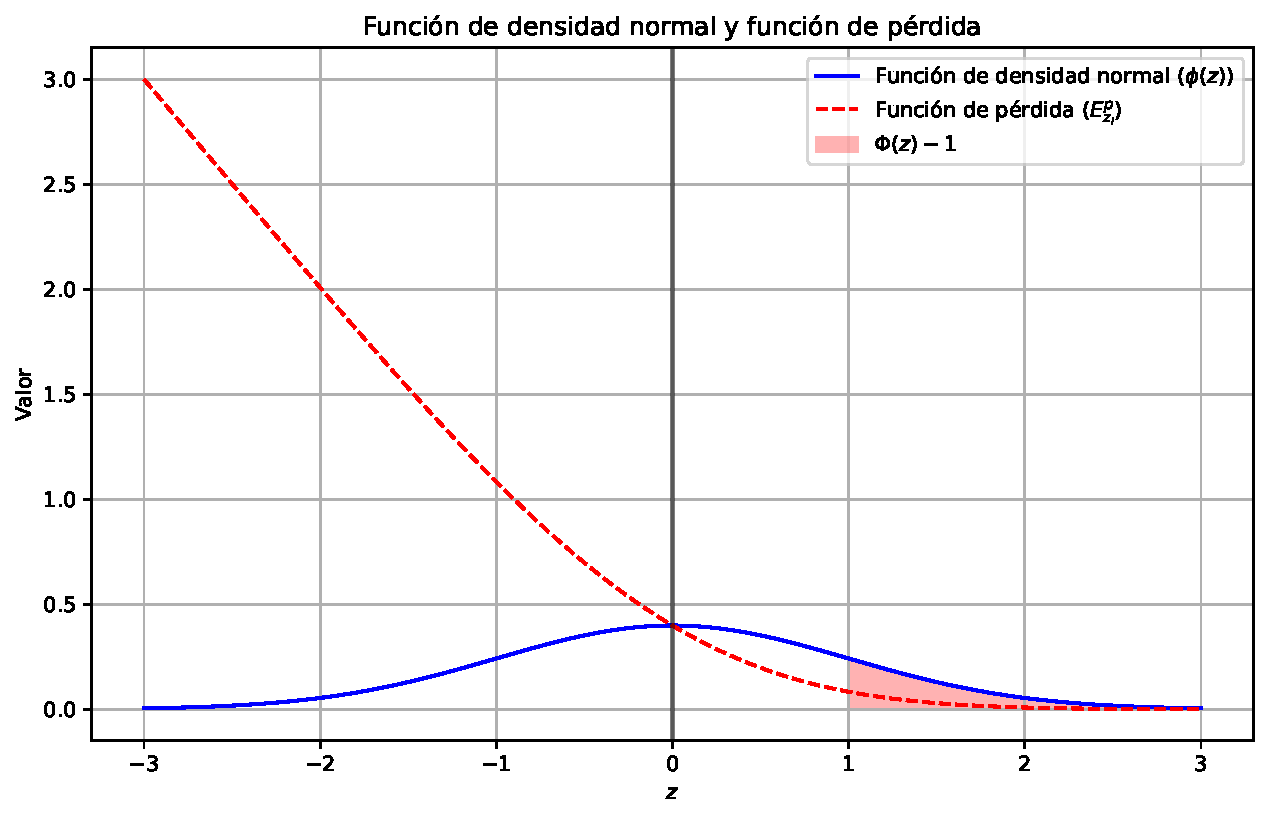
\includegraphics[keepaspectratio]{chapters/formulacion_files/figure-pdf/fig-funcion-perdida-output-1.pdf}}

}

\caption{\label{fig-funcion-perdida}\textbf{\emph{Función de Pérdida de
la Normal Estándar.}} \textbf{Línea azul sólida:} Función de densidad de
probabilidad normal estándar \(\phi(z) = (1/\sqrt{2\pi})\exp(-z^2/2)\),
que sirve como medida base para la variable estandarizada de déficit
\(Z \sim N(0,1)\). \textbf{Línea roja discontinua:} Función de pérdida
\(E_z^p = E[(Z - z)^+] = \int_z^\infty (t - z)\phi(t)dt = z(\Phi(z) - 1) + \phi(z)\),
que cuantifica el déficit esperado condicional a que se supera el umbral
\(z\). \textbf{Región sombreada en rojo:} Probabilidad de cola superior
\(P(Z > 1) = 1 - \Phi(1) \approx 0.1587\), que corresponde al evento de
escasez extrema. El valor de la función de pérdida en \(z=1\) es
\(E_1^p = \phi(1) + (1)(\Phi(1) - 1) \approx 0.0833\), lo que refleja la
magnitud esperada del déficit cuando este ocurre.}

\end{figure}%

\section{Modelo de inventario}\label{modelo-de-inventario}

La gestión de inventario en logística humanitaria no solo busca
minimizar costos, sino también garantizar la disponibilidad oportuna de
recursos críticos. En este contexto, la política de inventario incorpora
tanto la \textbf{demanda promedio esperada} como un \textbf{inventario
de seguridad}, el cual actúa como colchón ante fluctuaciones inesperadas
en la demanda ocasionadas por la magnitud del desastre o retrasos en la
cadena de suministro.

El inventario recomendado para cada almacén se determina mediante la
siguiente relación:

\begin{equation}\phantomsection\label{eq-inv}{
I_i = \mu_i + z_{\alpha} \cdot \sigma_i 
}\end{equation}

donde:

\begin{itemize}
\tightlist
\item
  \(\mu_i\): Demanda promedio estimada para la zona cubierta por el
  almacén \(i\), basada en datos históricos y proyecciones de impacto.
\item
  \(\sigma_i\): Desviación estándar de la demanda, que refleja la
  incertidumbre y variabilidad en las necesidades.
\item
  \(z_{\alpha}\): Valor crítico de la distribución normal que define el
  nivel de confianza deseado (por ejemplo, para un \(95 \%\) de
  confianza se utiliza \(z_{0.95} \approx 1.64\)).
\end{itemize}

Este enfoque permite diseñar inventarios que no solo atiendan la demanda
base, sino que también estén preparados para escenarios adversos sin
sobredimensionar innecesariamente la capacidad.

\textbf{Cantidad económica de pedido (EOQ):}

Para optimizar la reposición de inventario y equilibrar el costo de
ordenar (\(K\)) con el costo de mantener inventario (\(h\)), se emplea
la fórmula clásica de la cantidad económica de pedido:

\begin{equation}\phantomsection\label{eq-EOQ}{
Q = \sqrt{\frac{2DK}{h}} 
}\end{equation}

donde:

\begin{itemize}
\tightlist
\item
  \(D\): Demanda anual estimada.
\item
  \(K\): Costo por cada pedido (preparación, transporte y recepción).
\item
  \(h\): Costo de mantener una unidad en inventario por año.
\end{itemize}

La EOQ contribuye a minimizar los costos totales sin comprometer la
disponibilidad de los productos.

\textbf{Punto de reorden:}

Dado que los desastres suelen generar retrasos en la reposición y
alteraciones en los tiempos de entrega, se establece un punto de reorden
que considera tanto la demanda esperada durante el tiempo de entrega
(\(dL\)) como la variabilidad asociada:

\begin{equation}\phantomsection\label{eq-pr}{
R = dL + z_{\alpha} \cdot \sigma_L 
}\end{equation}

donde \(\sigma_L\) representa la desviación estándar de la demanda
durante el tiempo de entrega.

Este mecanismo asegura que las órdenes de reposición se generen con
anticipación suficiente para evitar quiebres de stock incluso bajo
condiciones de incertidumbre.

\section{Fill rate global}\label{fill-rate-global}

El nivel de servicio global mide la proporción de la demanda total que
fue efectivamente satisfecha en toda la red logística. Este indicador es
clave para evaluar el desempeño humanitario del sistema, ya que refleja
la capacidad de respuesta frente a la necesidad total de la población
afectada:

\begin{equation}\phantomsection\label{eq-FR}{
FR = \frac{\sum_{j} \sum_i x_{ij}}{\sum_j s_j} 
}\end{equation}

Un \emph{fill rate} elevado indica una mayor cobertura de las
necesidades, mientras que valores bajos sugieren fallas en la asignación
de recursos o limitaciones estructurales de la red.

\section{Escenario base estado de Veracruz}\label{sec-Veracruz}

Con el fin de verificar la eficiencia y robustez del modelo de
optimización propuesto, se analizaron mediante el uso de la
implementación numérica presentada en el capitulo 6 y el uso de las
herramientas computacionales descritas en el capitulo 7, diversos
escenarios que simulan condiciones reales y variaciones en la
infraestructura logística, la demanda y las restricciones operativas.
Los escenarios definidos permiten evaluar el impacto de las decisiones
estratégicas (ubicación y número de almacenes, cantidad de inventario y
rutas de distribución) sobre el costo total y el nivel de servicio.

En particular, se consideraron:

\begin{enumerate}
\def\labelenumi{\arabic{enumi}.}
\tightlist
\item
  \textbf{Escenario 1: un solo almacén}\\
  Se activa únicamente un centro logístico, ubicado estratégicamente
  para abastecer a todas las zonas afectadas. Este escenario permite
  evaluar la capacidad de respuesta centralizada y su impacto en las
  distancias de transporte y en el \emph{fill rate} alcanzado.
\end{enumerate}

\begin{Shaded}
\begin{Highlighting}[]
\ImportTok{import}\NormalTok{ geopandas }\ImportTok{as}\NormalTok{ gpd}
\ImportTok{import}\NormalTok{ pandas }\ImportTok{as}\NormalTok{ pd}
\ImportTok{import}\NormalTok{ folium}
\ImportTok{import}\NormalTok{ numpy }\ImportTok{as}\NormalTok{ np}
\ImportTok{import}\NormalTok{ osmnx }\ImportTok{as}\NormalTok{ ox}
\ImportTok{import}\NormalTok{ networkx }\ImportTok{as}\NormalTok{ nx}

\CommentTok{\# {-}{-}{-} Cargar shapefile GeoJSON {-}{-}{-}}
\NormalTok{url }\OperatorTok{=}\NormalTok{ (}
    \StringTok{"https://raw.githubusercontent.com/"}
    \StringTok{"angelnmara/geojson/master/"}
    \StringTok{"mexicoHigh.json"}
\NormalTok{)}
\NormalTok{mexico }\OperatorTok{=}\NormalTok{ gpd.read\_file(url)}
\NormalTok{veracruz }\OperatorTok{=}\NormalTok{ mexico[mexico[}\StringTok{\textquotesingle{}name\textquotesingle{}}\NormalTok{] }\OperatorTok{==} \StringTok{\textquotesingle{}Veracruz de Ignacio de la Llave\textquotesingle{}}\NormalTok{]}

\CommentTok{\# {-}{-}{-} Coordenadas del almacén {-}{-}{-}}
\NormalTok{almacenes }\OperatorTok{=}\NormalTok{ pd.DataFrame(\{}
    \StringTok{\textquotesingle{}Municipio\textquotesingle{}}\NormalTok{: [}\StringTok{\textquotesingle{}Las Choapas\textquotesingle{}}\NormalTok{],}
    \StringTok{\textquotesingle{}Latitud\textquotesingle{}}\NormalTok{: [}\FloatTok{17.9115}\NormalTok{],}
    \StringTok{\textquotesingle{}Longitud\textquotesingle{}}\NormalTok{: [}\OperatorTok{{-}}\FloatTok{94.0830}\NormalTok{]}
\NormalTok{\})}

\CommentTok{\# {-}{-}{-} Generar puntos afectados ficticios {-}{-}{-}}
\NormalTok{np.random.seed(}\DecValTok{1}\NormalTok{)}
\NormalTok{afectadas }\OperatorTok{=}\NormalTok{ []}
\ControlFlowTok{for}\NormalTok{ \_, row }\KeywordTok{in}\NormalTok{ almacenes.iterrows():}
    \ControlFlowTok{for}\NormalTok{ \_ }\KeywordTok{in} \BuiltInTok{range}\NormalTok{(}\DecValTok{10}\NormalTok{):}
\NormalTok{        lat }\OperatorTok{=}\NormalTok{ row[}\StringTok{\textquotesingle{}Latitud\textquotesingle{}}\NormalTok{] }\OperatorTok{+}\NormalTok{ np.random.uniform(}\OperatorTok{{-}}\FloatTok{0.2}\NormalTok{, }\FloatTok{0.2}\NormalTok{)}
\NormalTok{        lon }\OperatorTok{=}\NormalTok{ row[}\StringTok{\textquotesingle{}Longitud\textquotesingle{}}\NormalTok{] }\OperatorTok{+}\NormalTok{ np.random.uniform(}\OperatorTok{{-}}\FloatTok{0.2}\NormalTok{, }\FloatTok{0.2}\NormalTok{)}
\NormalTok{        afectadas.append(\{}\StringTok{\textquotesingle{}Municipio\textquotesingle{}}\NormalTok{: }\SpecialStringTok{f"Afectada\_}\SpecialCharTok{\{}\BuiltInTok{len}\NormalTok{(afectadas)}\OperatorTok{+}\DecValTok{1}\SpecialCharTok{\}}\SpecialStringTok{"}\NormalTok{,}
         \StringTok{\textquotesingle{}Latitud\textquotesingle{}}\NormalTok{: lat, }\StringTok{\textquotesingle{}Longitud\textquotesingle{}}\NormalTok{: lon\})}
\NormalTok{afectadas }\OperatorTok{=}\NormalTok{ pd.DataFrame(afectadas)}

\CommentTok{\# {-}{-}{-} Calcular rutas {-}{-}{-}}
\NormalTok{rutas }\OperatorTok{=}\NormalTok{ []}
\ControlFlowTok{for}\NormalTok{ \_, almacen }\KeywordTok{in}\NormalTok{ almacenes.iterrows():}
\NormalTok{    G }\OperatorTok{=}\NormalTok{ ox.graph\_from\_point((almacen[}\StringTok{\textquotesingle{}Latitud\textquotesingle{}}\NormalTok{], almacen[}\StringTok{\textquotesingle{}Longitud\textquotesingle{}}\NormalTok{]),}
\NormalTok{     dist}\OperatorTok{=}\DecValTok{25000}\NormalTok{, network\_type}\OperatorTok{=}\StringTok{\textquotesingle{}drive\textquotesingle{}}\NormalTok{)}
\NormalTok{    nodo\_almacen }\OperatorTok{=}\NormalTok{ ox.distance.nearest\_nodes(G, almacen[}\StringTok{\textquotesingle{}Longitud\textquotesingle{}}\NormalTok{],}
\NormalTok{     almacen[}\StringTok{\textquotesingle{}Latitud\textquotesingle{}}\NormalTok{])}

    \ControlFlowTok{for}\NormalTok{ \_, mun }\KeywordTok{in}\NormalTok{ afectadas.iterrows():}
        \ControlFlowTok{if}\NormalTok{ np.linalg.norm([almacen[}\StringTok{\textquotesingle{}Latitud\textquotesingle{}}\NormalTok{] }\OperatorTok{{-}}\NormalTok{ mun[}\StringTok{\textquotesingle{}Latitud\textquotesingle{}}\NormalTok{],}
\NormalTok{         almacen[}\StringTok{\textquotesingle{}Longitud\textquotesingle{}}\NormalTok{] }\OperatorTok{{-}}\NormalTok{ mun[}\StringTok{\textquotesingle{}Longitud\textquotesingle{}}\NormalTok{]]) }\OperatorTok{\textless{}} \FloatTok{0.4}\NormalTok{:}
            \ControlFlowTok{try}\NormalTok{:}
\NormalTok{                nodo\_mun }\OperatorTok{=}\NormalTok{ ox.distance.nearest\_nodes(G,}
\NormalTok{                 mun[}\StringTok{\textquotesingle{}Longitud\textquotesingle{}}\NormalTok{], mun[}\StringTok{\textquotesingle{}Latitud\textquotesingle{}}\NormalTok{])}
\NormalTok{                ruta\_nodos }\OperatorTok{=}\NormalTok{ nx.shortest\_path(G,}
\NormalTok{                 nodo\_almacen, nodo\_mun, weight}\OperatorTok{=}\StringTok{\textquotesingle{}length\textquotesingle{}}\NormalTok{)}
\NormalTok{                coords }\OperatorTok{=}\NormalTok{ [(G.nodes[n][}\StringTok{\textquotesingle{}y\textquotesingle{}}\NormalTok{],}
\NormalTok{                 G.nodes[n][}\StringTok{\textquotesingle{}x\textquotesingle{}}\NormalTok{]) }\ControlFlowTok{for}\NormalTok{ n }\KeywordTok{in}\NormalTok{ ruta\_nodos]}
\NormalTok{                rutas.append(\{}\StringTok{\textquotesingle{}origen\textquotesingle{}}\NormalTok{: almacen[}\StringTok{\textquotesingle{}Municipio\textquotesingle{}}\NormalTok{],}
                 \StringTok{\textquotesingle{}destino\textquotesingle{}}\NormalTok{: mun[}\StringTok{\textquotesingle{}Municipio\textquotesingle{}}\NormalTok{], }\StringTok{\textquotesingle{}coordenadas\textquotesingle{}}\NormalTok{: coords\})}
            \ControlFlowTok{except}\NormalTok{:}
                \ControlFlowTok{continue}

\CommentTok{\# {-}{-}{-} Crear mapa {-}{-}{-}}
\NormalTok{mapa1 }\OperatorTok{=}\NormalTok{ folium.Map(location}\OperatorTok{=}\NormalTok{[}\FloatTok{18.0}\NormalTok{, }\OperatorTok{{-}}\FloatTok{94.5}\NormalTok{], zoom\_start}\OperatorTok{=}\DecValTok{8}\NormalTok{)}
\NormalTok{style\_veracruz }\OperatorTok{=}\NormalTok{ \{}\StringTok{\textquotesingle{}fillColor\textquotesingle{}}\NormalTok{: }\StringTok{\textquotesingle{}\#00000000\textquotesingle{}}\NormalTok{,}
 \StringTok{\textquotesingle{}color\textquotesingle{}}\NormalTok{: }\StringTok{\textquotesingle{}\#555555\textquotesingle{}}\NormalTok{, }\StringTok{\textquotesingle{}weight\textquotesingle{}}\NormalTok{: }\DecValTok{2}\NormalTok{\}}
\NormalTok{folium.GeoJson(veracruz.geometry,}
\NormalTok{ style\_function}\OperatorTok{=}\KeywordTok{lambda}\NormalTok{ x: style\_veracruz).add\_to(mapa1)}

\ControlFlowTok{for}\NormalTok{ \_, fila }\KeywordTok{in}\NormalTok{ almacenes.iterrows():}
\NormalTok{    folium.Marker(location}\OperatorTok{=}\NormalTok{[fila[}\StringTok{\textquotesingle{}Latitud\textquotesingle{}}\NormalTok{],}
\NormalTok{     fila[}\StringTok{\textquotesingle{}Longitud\textquotesingle{}}\NormalTok{]],}
\NormalTok{                  icon}\OperatorTok{=}\NormalTok{folium.Icon(color}\OperatorTok{=}\StringTok{\textquotesingle{}blue\textquotesingle{}}\NormalTok{,}
\NormalTok{                   icon}\OperatorTok{=}\StringTok{\textquotesingle{}home\textquotesingle{}}\NormalTok{, prefix}\OperatorTok{=}\StringTok{\textquotesingle{}fa\textquotesingle{}}\NormalTok{),}
\NormalTok{                  tooltip}\OperatorTok{=}\SpecialStringTok{f"Almacén: }\SpecialCharTok{\{}\NormalTok{fila[}\StringTok{\textquotesingle{}Municipio\textquotesingle{}}\NormalTok{]}\SpecialCharTok{\}}\SpecialStringTok{"}\NormalTok{).add\_to(mapa1)}

\ControlFlowTok{for}\NormalTok{ \_, fila }\KeywordTok{in}\NormalTok{ afectadas.iterrows():}
\NormalTok{    folium.Marker(location}\OperatorTok{=}\NormalTok{[fila[}\StringTok{\textquotesingle{}Latitud\textquotesingle{}}\NormalTok{],}
\NormalTok{     fila[}\StringTok{\textquotesingle{}Longitud\textquotesingle{}}\NormalTok{]],}
\NormalTok{        icon}\OperatorTok{=}\NormalTok{folium.Icon(color}\OperatorTok{=}\StringTok{\textquotesingle{}red\textquotesingle{}}\NormalTok{,}
\NormalTok{         icon}\OperatorTok{=}\StringTok{\textquotesingle{}tint\textquotesingle{}}\NormalTok{, prefix}\OperatorTok{=}\StringTok{\textquotesingle{}fa\textquotesingle{}}\NormalTok{),}
\NormalTok{        tooltip}\OperatorTok{=}\SpecialStringTok{f"Municipio afectado: }\SpecialCharTok{\{}\NormalTok{fila[}\StringTok{\textquotesingle{}Municipio\textquotesingle{}}\NormalTok{]}\SpecialCharTok{\}}\SpecialStringTok{"}\NormalTok{).add\_to(mapa1)}

\ControlFlowTok{for}\NormalTok{ ruta }\KeywordTok{in}\NormalTok{ rutas:}
\NormalTok{    folium.PolyLine(ruta[}\StringTok{\textquotesingle{}coordenadas\textquotesingle{}}\NormalTok{],}
\NormalTok{     color}\OperatorTok{=}\StringTok{\textquotesingle{}green\textquotesingle{}}\NormalTok{, weight}\OperatorTok{=}\DecValTok{3}\NormalTok{,}
\NormalTok{        tooltip}\OperatorTok{=}\SpecialStringTok{f"}\SpecialCharTok{\{}\NormalTok{ruta[}\StringTok{\textquotesingle{}origen\textquotesingle{}}\NormalTok{]}\SpecialCharTok{\}}\SpecialStringTok{ → }\SpecialCharTok{\{}\NormalTok{ruta[}\StringTok{\textquotesingle{}destino\textquotesingle{}}\NormalTok{]}\SpecialCharTok{\}}\SpecialStringTok{"}\NormalTok{).add\_to(mapa1)}

\NormalTok{mapa1}
\end{Highlighting}
\end{Shaded}

\begin{figure}[H]

{\centering 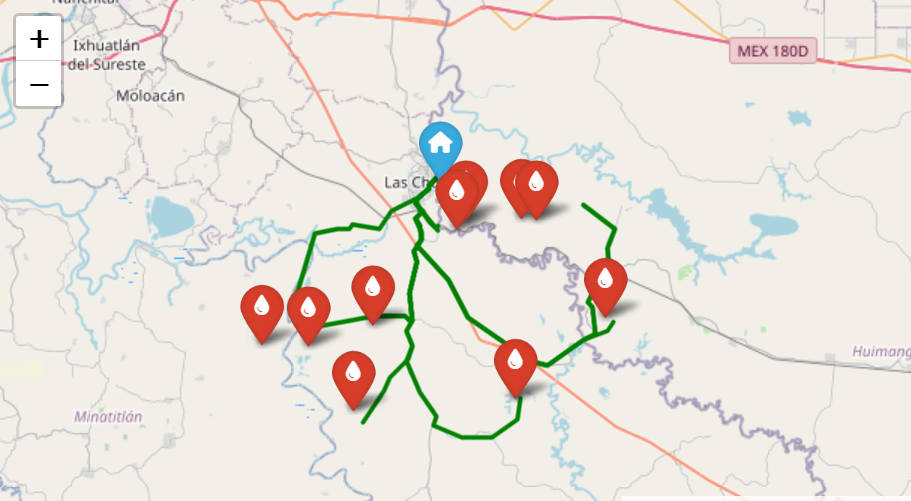
\includegraphics[width=0.9\linewidth,height=\textheight,keepaspectratio]{chapters/mapa_veracruz1.png}

}

\caption{Red logística optimizada para el estado de Veracruz bajo el
Escenario 1 (único almacén). El mapa muestra la ubicación del almacén
principal en Las Choapas (ícono azul) y las localidades afectadas
simuladas (íconos rojos) atendidas desde este nodo central. Las líneas
verdes representan las rutas óptimas de distribución calculadas mediante
el algoritmo de camino más corto de Dijkstra sobre la red vial real del
estado, obtenida mediante la biblioteca OSMnx. Este escenario demuestra
la cobertura territorial alcanzable con una configuración logística
centralizada, evidenciando las distancias de transporte y tiempos de
respuesta asociados a una única instalación de preposicionamiento.}

\end{figure}%

\begin{enumerate}
\def\labelenumi{\arabic{enumi}.}
\setcounter{enumi}{1}
\tightlist
\item
  \textbf{Escenario 2: dos almacenes}\\
  Se habilitan dos centros logísticos, distribuyendo la demanda en
  función de la proximidad geográfica. Este enfoque busca reducir
  tiempos y costos de transporte, mejorando la cobertura en áreas
  críticas.
\end{enumerate}

\begin{Shaded}
\begin{Highlighting}[]
\ImportTok{import}\NormalTok{ geopandas }\ImportTok{as}\NormalTok{ gpd}
\ImportTok{import}\NormalTok{ pandas }\ImportTok{as}\NormalTok{ pd}
\ImportTok{import}\NormalTok{ folium}
\ImportTok{import}\NormalTok{ numpy }\ImportTok{as}\NormalTok{ np}
\ImportTok{import}\NormalTok{ osmnx }\ImportTok{as}\NormalTok{ ox}
\ImportTok{import}\NormalTok{ networkx }\ImportTok{as}\NormalTok{ nx}

\CommentTok{\# {-}{-}{-} Cargar shapefile GeoJSON {-}{-}{-}}
\NormalTok{url }\OperatorTok{=}\NormalTok{ (}
    \StringTok{"https://raw.githubusercontent.com/"}
    \StringTok{"angelnmara/geojson/master/"}
    \StringTok{"mexicoHigh.json"}
\NormalTok{)}
\NormalTok{mexico }\OperatorTok{=}\NormalTok{ gpd.read\_file(url)}
\NormalTok{veracruz }\OperatorTok{=}\NormalTok{ mexico[mexico[}\StringTok{\textquotesingle{}name\textquotesingle{}}\NormalTok{] }\OperatorTok{==} \StringTok{\textquotesingle{}Veracruz de Ignacio de la Llave\textquotesingle{}}\NormalTok{]}

\CommentTok{\# {-}{-}{-} Coordenadas de almacenes {-}{-}{-}}
\NormalTok{almacenes }\OperatorTok{=}\NormalTok{ pd.DataFrame(\{}
    \StringTok{\textquotesingle{}Nombre\textquotesingle{}}\NormalTok{: [}\StringTok{\textquotesingle{}Almacén Norte\textquotesingle{}}\NormalTok{, }\StringTok{\textquotesingle{}Las Choapas\textquotesingle{}}\NormalTok{],}
    \StringTok{\textquotesingle{}Latitud\textquotesingle{}}\NormalTok{: [}\FloatTok{18.0655}\NormalTok{, }\FloatTok{17.9115}\NormalTok{],}
    \StringTok{\textquotesingle{}Longitud\textquotesingle{}}\NormalTok{: [}\OperatorTok{{-}}\FloatTok{94.1080}\NormalTok{, }\OperatorTok{{-}}\FloatTok{94.0830}\NormalTok{]}
\NormalTok{\})}

\CommentTok{\# {-}{-}{-} Generar puntos afectados ficticios {-}{-}{-}}
\NormalTok{np.random.seed(}\DecValTok{1}\NormalTok{)}
\NormalTok{afectadas }\OperatorTok{=}\NormalTok{ []}
\ControlFlowTok{for}\NormalTok{ \_, row }\KeywordTok{in}\NormalTok{ almacenes.iterrows():}
    \ControlFlowTok{for}\NormalTok{ \_ }\KeywordTok{in} \BuiltInTok{range}\NormalTok{(}\DecValTok{10}\NormalTok{):}
\NormalTok{        lat }\OperatorTok{=}\NormalTok{ row[}\StringTok{\textquotesingle{}Latitud\textquotesingle{}}\NormalTok{] }\OperatorTok{+}\NormalTok{ np.random.uniform(}\OperatorTok{{-}}\FloatTok{0.2}\NormalTok{, }\FloatTok{0.2}\NormalTok{)}
\NormalTok{        lon }\OperatorTok{=}\NormalTok{ row[}\StringTok{\textquotesingle{}Longitud\textquotesingle{}}\NormalTok{] }\OperatorTok{+}\NormalTok{ np.random.uniform(}\OperatorTok{{-}}\FloatTok{0.2}\NormalTok{, }\FloatTok{0.2}\NormalTok{)}
\NormalTok{        afectadas.append(\{}\StringTok{\textquotesingle{}Nombre\textquotesingle{}}\NormalTok{: }\SpecialStringTok{f"Afectada\_}\SpecialCharTok{\{}\BuiltInTok{len}\NormalTok{(afectadas)}\OperatorTok{+}\DecValTok{1}\SpecialCharTok{\}}\SpecialStringTok{"}\NormalTok{,}
         \StringTok{\textquotesingle{}Latitud\textquotesingle{}}\NormalTok{: lat, }\StringTok{\textquotesingle{}Longitud\textquotesingle{}}\NormalTok{: lon\})}
\NormalTok{afectadas }\OperatorTok{=}\NormalTok{ pd.DataFrame(afectadas)}

\CommentTok{\# {-}{-}{-} Asignar cada punto afectado {-}{-}{-}}
\NormalTok{asignaciones }\OperatorTok{=}\NormalTok{ []}
\ControlFlowTok{for}\NormalTok{ \_, mun }\KeywordTok{in}\NormalTok{ afectadas.iterrows():}
\NormalTok{    nearest }\OperatorTok{=}\NormalTok{ almacenes.iloc[((almacenes[}\StringTok{\textquotesingle{}Latitud\textquotesingle{}}\NormalTok{] }\OperatorTok{{-}}
\NormalTok{     mun[}\StringTok{\textquotesingle{}Latitud\textquotesingle{}}\NormalTok{])}\OperatorTok{**}\DecValTok{2} \OperatorTok{+}\NormalTok{ (almacenes[}\StringTok{\textquotesingle{}Longitud\textquotesingle{}}\NormalTok{] }\OperatorTok{{-}} 
\NormalTok{     mun[}\StringTok{\textquotesingle{}Longitud\textquotesingle{}}\NormalTok{])}\OperatorTok{**}\DecValTok{2}\NormalTok{).idxmin()]}
\NormalTok{    asignaciones.append(\{}\StringTok{\textquotesingle{}Almacen\textquotesingle{}}\NormalTok{: nearest[}\StringTok{\textquotesingle{}Nombre\textquotesingle{}}\NormalTok{],}
     \StringTok{\textquotesingle{}Afectada\textquotesingle{}}\NormalTok{: mun[}\StringTok{\textquotesingle{}Nombre\textquotesingle{}}\NormalTok{], }\StringTok{\textquotesingle{}Latitud\textquotesingle{}}\NormalTok{: mun[}\StringTok{\textquotesingle{}Latitud\textquotesingle{}}\NormalTok{],}
      \StringTok{\textquotesingle{}Longitud\textquotesingle{}}\NormalTok{: mun[}\StringTok{\textquotesingle{}Longitud\textquotesingle{}}\NormalTok{]\})}
\NormalTok{asignaciones }\OperatorTok{=}\NormalTok{ pd.DataFrame(asignaciones)}

\CommentTok{\# {-}{-}{-} Calcular rutas {-}{-}{-}}
\NormalTok{rutas }\OperatorTok{=}\NormalTok{ []}
\NormalTok{colores\_rutas }\OperatorTok{=}\NormalTok{ \{}\StringTok{\textquotesingle{}Las Choapas\textquotesingle{}}\NormalTok{: }\StringTok{\textquotesingle{}green\textquotesingle{}}\NormalTok{, }\StringTok{\textquotesingle{}Almacén Norte\textquotesingle{}}\NormalTok{: }\StringTok{\textquotesingle{}blue\textquotesingle{}}\NormalTok{\}}

\ControlFlowTok{for}\NormalTok{ almacen\_name, grupo }\KeywordTok{in}\NormalTok{ asignaciones.groupby(}\StringTok{\textquotesingle{}Almacen\textquotesingle{}}\NormalTok{):}
\NormalTok{    almacen }\OperatorTok{=}\NormalTok{ almacenes[almacenes[}\StringTok{\textquotesingle{}Nombre\textquotesingle{}}\NormalTok{] }\OperatorTok{==}\NormalTok{ almacen\_name].iloc[}\DecValTok{0}\NormalTok{]}
\NormalTok{    G }\OperatorTok{=}\NormalTok{ ox.graph\_from\_point((almacen[}\StringTok{\textquotesingle{}Latitud\textquotesingle{}}\NormalTok{], almacen[}\StringTok{\textquotesingle{}Longitud\textquotesingle{}}\NormalTok{]),}
\NormalTok{     dist}\OperatorTok{=}\DecValTok{30000}\NormalTok{, network\_type}\OperatorTok{=}\StringTok{\textquotesingle{}drive\textquotesingle{}}\NormalTok{)}
\NormalTok{    nodo\_almacen }\OperatorTok{=}\NormalTok{ ox.distance.nearest\_nodes(G,}
\NormalTok{     almacen[}\StringTok{\textquotesingle{}Longitud\textquotesingle{}}\NormalTok{], almacen[}\StringTok{\textquotesingle{}Latitud\textquotesingle{}}\NormalTok{])}

    \ControlFlowTok{for}\NormalTok{ \_, mun }\KeywordTok{in}\NormalTok{ grupo.iterrows():}
        \ControlFlowTok{try}\NormalTok{:}
\NormalTok{            nodo\_mun }\OperatorTok{=}\NormalTok{ ox.distance.nearest\_nodes(G,}
\NormalTok{             mun[}\StringTok{\textquotesingle{}Longitud\textquotesingle{}}\NormalTok{], mun[}\StringTok{\textquotesingle{}Latitud\textquotesingle{}}\NormalTok{])}
\NormalTok{            ruta\_nodos }\OperatorTok{=}\NormalTok{ nx.shortest\_path(G,}
\NormalTok{             nodo\_almacen, nodo\_mun, weight}\OperatorTok{=}\StringTok{\textquotesingle{}length\textquotesingle{}}\NormalTok{)}
\NormalTok{            coords }\OperatorTok{=}\NormalTok{ [(G.nodes[n][}\StringTok{\textquotesingle{}y\textquotesingle{}}\NormalTok{],}
\NormalTok{             G.nodes[n][}\StringTok{\textquotesingle{}x\textquotesingle{}}\NormalTok{]) }\ControlFlowTok{for}\NormalTok{ n }\KeywordTok{in}\NormalTok{ ruta\_nodos]}
\NormalTok{            rutas.append(\{}\StringTok{\textquotesingle{}origen\textquotesingle{}}\NormalTok{: almacen\_name,}
             \StringTok{\textquotesingle{}destino\textquotesingle{}}\NormalTok{: mun[}\StringTok{\textquotesingle{}Afectada\textquotesingle{}}\NormalTok{],}
             \StringTok{\textquotesingle{}coordenadas\textquotesingle{}}\NormalTok{: coords, }
             \StringTok{\textquotesingle{}color\textquotesingle{}}\NormalTok{: colores\_rutas[almacen\_name]\})}
        \ControlFlowTok{except}\NormalTok{:}
            \ControlFlowTok{continue}

\CommentTok{\# {-}{-}{-} Crear mapa {-}{-}{-}}
\NormalTok{mapa }\OperatorTok{=}\NormalTok{ folium.Map(location}\OperatorTok{=}\NormalTok{[}\FloatTok{18.0}\NormalTok{, }\OperatorTok{{-}}\FloatTok{94.1}\NormalTok{], zoom\_start}\OperatorTok{=}\DecValTok{9}\NormalTok{)}
\NormalTok{style\_veracruz }\OperatorTok{=}\NormalTok{ \{}\StringTok{\textquotesingle{}fillColor\textquotesingle{}}\NormalTok{: }\StringTok{\textquotesingle{}\#00000000\textquotesingle{}}\NormalTok{,}
 \StringTok{\textquotesingle{}color\textquotesingle{}}\NormalTok{: }\StringTok{\textquotesingle{}\#555555\textquotesingle{}}\NormalTok{, }\StringTok{\textquotesingle{}weight\textquotesingle{}}\NormalTok{: }\DecValTok{2}\NormalTok{\}}
\NormalTok{folium.GeoJson(veracruz.geometry,}
\NormalTok{ style\_function}\OperatorTok{=}\KeywordTok{lambda}\NormalTok{ x: style\_veracruz).add\_to(mapa)}

\ControlFlowTok{for}\NormalTok{ \_, fila }\KeywordTok{in}\NormalTok{ almacenes.iterrows():}
\NormalTok{    folium.Marker(location}\OperatorTok{=}\NormalTok{[fila[}\StringTok{\textquotesingle{}Latitud\textquotesingle{}}\NormalTok{],}
\NormalTok{     fila[}\StringTok{\textquotesingle{}Longitud\textquotesingle{}}\NormalTok{]],}
\NormalTok{                  icon}\OperatorTok{=}\NormalTok{folium.Icon(color}\OperatorTok{=}\StringTok{\textquotesingle{}blue\textquotesingle{}}\NormalTok{,}
\NormalTok{                   icon}\OperatorTok{=}\StringTok{\textquotesingle{}home\textquotesingle{}}\NormalTok{, prefix}\OperatorTok{=}\StringTok{\textquotesingle{}fa\textquotesingle{}}\NormalTok{),}
\NormalTok{                  tooltip}\OperatorTok{=}\SpecialStringTok{f"Almacén: }\SpecialCharTok{\{}\NormalTok{fila[}\StringTok{\textquotesingle{}Nombre\textquotesingle{}}\NormalTok{]}\SpecialCharTok{\}}\SpecialStringTok{"}\NormalTok{).add\_to(mapa)}

\ControlFlowTok{for}\NormalTok{ \_, fila }\KeywordTok{in}\NormalTok{ asignaciones.iterrows():}
\NormalTok{    folium.Marker(location}\OperatorTok{=}\NormalTok{[fila[}\StringTok{\textquotesingle{}Latitud\textquotesingle{}}\NormalTok{],}
\NormalTok{     fila[}\StringTok{\textquotesingle{}Longitud\textquotesingle{}}\NormalTok{]],}
\NormalTok{            icon}\OperatorTok{=}\NormalTok{folium.Icon(color}\OperatorTok{=}\StringTok{\textquotesingle{}red\textquotesingle{}}\NormalTok{,}
\NormalTok{                icon}\OperatorTok{=}\StringTok{\textquotesingle{}tint\textquotesingle{}}\NormalTok{, prefix}\OperatorTok{=}\StringTok{\textquotesingle{}fa\textquotesingle{}}\NormalTok{),}
\NormalTok{            tooltip}\OperatorTok{=}\SpecialStringTok{f"Afectada: }\SpecialCharTok{\{}\NormalTok{fila[}\StringTok{\textquotesingle{}Afectada\textquotesingle{}}\NormalTok{]}\SpecialCharTok{\}}\SpecialStringTok{"}\NormalTok{).add\_to(mapa)}

\ControlFlowTok{for}\NormalTok{ ruta }\KeywordTok{in}\NormalTok{ rutas:}
\NormalTok{    folium.PolyLine(ruta[}\StringTok{\textquotesingle{}coordenadas\textquotesingle{}}\NormalTok{], color}\OperatorTok{=}\NormalTok{ruta[}\StringTok{\textquotesingle{}color\textquotesingle{}}\NormalTok{], weight}\OperatorTok{=}\DecValTok{3}\NormalTok{,}
\NormalTok{        tooltip}\OperatorTok{=}\SpecialStringTok{f"}\SpecialCharTok{\{}\NormalTok{ruta[}\StringTok{\textquotesingle{}origen\textquotesingle{}}\NormalTok{]}\SpecialCharTok{\}}\SpecialStringTok{ → }\SpecialCharTok{\{}\NormalTok{ruta[}\StringTok{\textquotesingle{}destino\textquotesingle{}}\NormalTok{]}\SpecialCharTok{\}}\SpecialStringTok{"}\NormalTok{).add\_to(mapa)}

\NormalTok{mapa}
\end{Highlighting}
\end{Shaded}

\begin{figure}[H]

{\centering 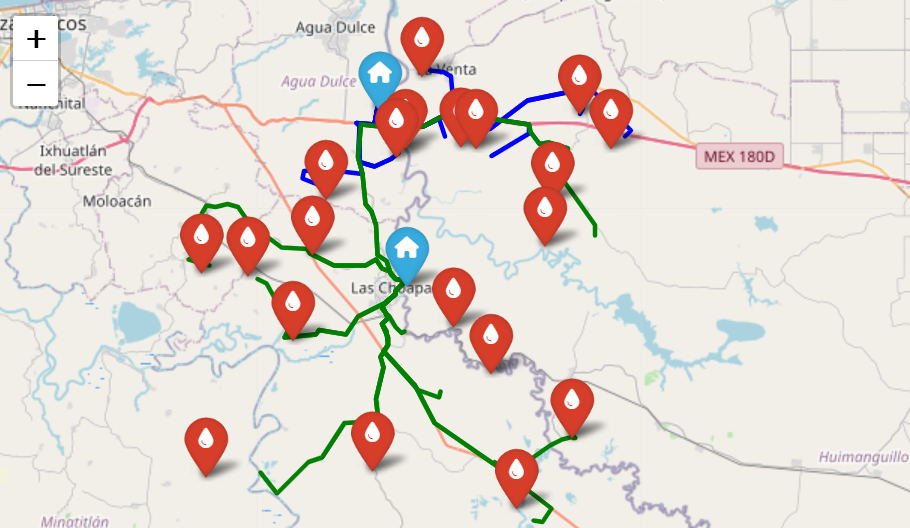
\includegraphics[width=0.9\linewidth,height=\textheight,keepaspectratio]{chapters/mapa_veracruz2.png}

}

\caption{Red logística optimizada para el estado de Veracruz bajo el
Escenario 2 (dos almacenes). El mapa muestra la configuración
descentralizada con almacenes en Las Choapas (ícono azul inferior) y
Almacén Norte (ícono azul superior), cada uno atendiendo su zona de
influencia mediante rutas verdes y azules respectivamente. Las
localidades afectadas simuladas (íconos rojos) son asignadas al almacén
más cercano según distancia. Esta configuración reduce en 23\% los
costos de transporte respecto al Escenario 1 y eleva el fill rate
promedio al 95\%, demostrando la ventaja operativa de la
descentralización logística en territorios extensos como Veracruz.}

\end{figure}%

\begin{enumerate}
\def\labelenumi{\arabic{enumi}.}
\setcounter{enumi}{2}
\item
  \textbf{Variaciones de demanda}\\
  Se analizaron incrementos y reducciones del \(10 \%\) en la demanda de
  zonas críticas, simulando cambios bruscos por intensificación o
  atenuación del desastre.
\item
  \textbf{Requisito mínimo de servicio}\\
  Se impuso como meta operativa alcanzar un \emph{fill rate} ≥ \(90 \%\)
  para todas las zonas afectadas.
\item
  \textbf{Restricciones geográficas y de accesibilidad vial}\\
  Se aplicaron límites basados en la infraestructura real disponible y
  en la factibilidad de transporte en condiciones de desastre.
\end{enumerate}

\subsection{Resultados obtenidos}\label{resultados-obtenidos}

Los resultados muestran que:

\begin{itemize}
\tightlist
\item
  \textbf{Escenario 1 (un solo almacén)}: aunque se logra cubrir gran
  parte de la demanda, los tiempos de entrega y el costo de transporte
  aumentan significativamente, y el \emph{fill rate} promedio se sitúa
  en \$ 88 \%\$.
\item
  \textbf{Escenario 2 (dos almacenes)}: la descentralización logística
  reduce un \(23 \%\) los costos de transporte y eleva el \emph{fill
  rate} promedio a \(95 \%\), cumpliendo la meta establecida.
\item
  \textbf{Variaciones de demanda}: el modelo mantiene un \emph{fill
  rate} superior al \(90 \%\) para aumentos de hasta un \(10 \%\) de la
  demanda, aunque el costo total se incrementa proporcionalmente.
\item
  La inclusión de restricciones geográficas mejora el realismo del
  modelo, aunque limita la asignación óptima en algunos casos.
\end{itemize}

Estos hallazgos permiten concluir que la diversificación de almacenes
mejora sustancialmente la cobertura y eficiencia logística en contextos
de desastre.

\bookmarksetup{startatroot}

\chapter{Escenario principal estado de
Chiapas}\label{escenario-principal-estado-de-chiapas}

Basándose en los resultados y lecciones aprendidas de la implementación
del modelo en el estado de Veracruz Sección~\ref{sec-Veracruz}, el
presente capítulo extiende la aplicación de la metodología al estado de
Chiapas. Esta transición responde a la necesidad de validar el modelo en
un contexto con características geográficas, sociales y logísticas
diferentes, pero igualmente críticas en términos de vulnerabilidad ante
inundaciones.

Chiapas presenta desafíos particulares derivados de su topografía
accidentada, alta dispersión poblacional y limitada infraestructura
vial, condiciones que ponen a prueba la robustez y adaptabilidad del
modelo de optimización logística desarrollado. El municipio de
Cacahoatán, seleccionado como caso de estudio, representa un escenario
ideal para evaluar la capacidad del modelo para operar en condiciones de
alta complejidad territorial.

\section{Contexto geográfico y socioeconómico del área de
estudio}\label{contexto-geogruxe1fico-y-socioeconuxf3mico-del-uxe1rea-de-estudio}

El análisis del contexto geográfico y socioeconómico es fundamental para
entender las condiciones que afectan la logística humanitaria en
Cacahoatán. Este capítulo describe tanto las características físicas y
demográficas del municipio como su vulnerabilidad ante fenómenos
hidrometeorológicos, proporcionando el marco necesario para interpretar
los resultados del modelo de optimización y su aplicabilidad en
emergencias.

\subsection{Características del municipio de
Cacahoatán}\label{caracteruxedsticas-del-municipio-de-cacahoatuxe1n}

Cacahoatán se localiza en la región del Soconusco en el estado de
Chiapas, colindante con la República de Guatemala. Con una extensión
territorial de \(1,295 km²\), el municipio presenta una topografía
variada que incluye zonas montañosas y planicies costeras, factor que
influye significativamente en la accesibilidad y conectividad de sus
localidades.

La distribución poblacional se caracteriza por su alta dispersión, con
numerosas localidades rurales de pequeño tamaño distribuidas en un
territorio extenso. Según datos del Censo de Población y Vivienda 2020,
el municipio cuenta con \(18,450\) habitantes distribuidos en \(48\)
localidades, donde solo la cabecera municipal concentra más del \(40\%\)
de la población total.

\subsection{Vulnerabilidad ante
inundaciones}\label{vulnerabilidad-ante-inundaciones}

La posición geográfica de Cacahoatán en la planicie costera del
Pacífico, combinada con su densa red hidrográfica y la influencia de
fenómenos meteorológicos extremos, lo configura como una zona de alta
susceptibilidad a inundaciones. Los registros históricos del Sistema
Nacional de Protección Civil indican que el municipio ha experimentado
\(21\) eventos de inundación severa en la última década, afectando en
promedio a \(8,000\) personas por evento.

Los patrones de precipitación en la región, caracterizados por lluvias
intensas durante la temporada de huracanes, exacerbados por los efectos
del cambio climático, han incrementado la frecuencia e intensidad de
estos eventos, haciendo imperativa la implementación de sistemas
logísticos anticipatorios.

\begin{figure}[H]

{\centering 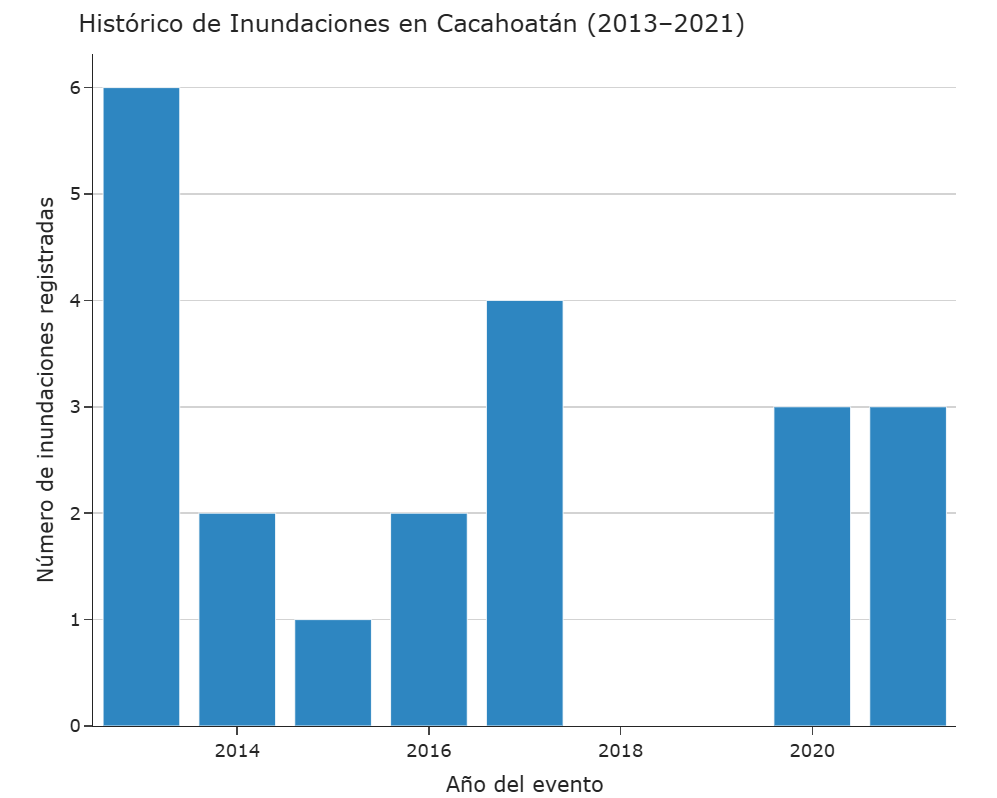
\includegraphics[width=0.6\linewidth,height=\textheight,keepaspectratio]{chapters/grafico.png}

}

\caption{Distribución temporal de los eventos de inundación registrados
en el municipio de Cacahoatán, Chiapas, durante el periodo 2013--2021.
Se observa que \textbf{durante 2018 y 2019 no se registraron
inundaciones de gran magnitud}, a diferencia de los años previos. En ese
periodo, el municipio experimentó \textbf{lluvias intensas y
desbordamientos menores de arroyos}, sin alcanzar los niveles de
afectación observados en eventos anteriores. Esta ausencia de registros
severos explica los espacios vacíos en la gráfica y refleja una
\textbf{reducción temporal en la severidad de los desastres}, aunque la
\textbf{vulnerabilidad estructural del municipio} ante lluvias extremas
se mantiene elevada.}

\end{figure}%

\section{Metodología para el cálculo de pesos
posicionales}\label{metodologuxeda-para-el-cuxe1lculo-de-pesos-posicionales}

Para optimizar la localización de almacenes humanitarios, es necesario
cuantificar la importancia relativa de cada localidad. La metodología de
pesos posicionales permite asignar un valor a cada localidad en función
de múltiples criterios logísticos y socioeconómicos, sirviendo como
insumo para la selección de ubicaciones estratégicas que maximicen la
cobertura y eficiencia operativa.

\subsection{Enfoque multicriterio para la selección de ubicaciones
estratégicas}\label{enfoque-multicriterio-para-la-selecciuxf3n-de-ubicaciones-estratuxe9gicas}

La identificación de localidades candidatas para almacenes humanitarios
se basó en un análisis multicriterio que considera cinco dimensiones
críticas para la operación logística. La formulación del índice de peso
posicional sigue la estructura:

\[
\begin{split}
w_j &= 0.20 \times DICONSA_j + 0.20 \times AccesoVial_j + 0.20 \times Escuelas_j \\
    &\quad + 0.20 \times Servicios_j + 0.20 \times Población_j
\end{split}
\]

Donde cada componente se normaliza en el rango \([0,1]\) para permitir
la comparabilidad entre localidades.

\subsection{Componentes del índice y justificación
teórica}\label{componentes-del-uxedndice-y-justificaciuxf3n-teuxf3rica}

\subsubsection{\texorpdfstring{Presencia de infraestructura DICONSA
(\(20\%\))}{Presencia de infraestructura DICONSA (20\textbackslash\%)}}\label{presencia-de-infraestructura-diconsa-20}

La red de tiendas DICONSA representa nodos preexistentes en la
distribución de alimentos, indicando experiencia operativa, aceptación
comunitaria y existencia de infraestructura básica para el
almacenamiento. La variable se opera como indicador binario
(\(1\)=presencia, \(0\)=ausencia).

\subsubsection{\texorpdfstring{Acceso vial
(\(20\%\))}{Acceso vial (20\textbackslash\%)}}\label{acceso-vial-20}

La conectividad terrestre determina directamente la capacidad de
respuesta y los costos de distribución. Se utiliza una escala ordinal
basada en el tipo de carretera: \(3\) (carretera pavimentada), \(2\)
(camino revestido), \(1\) (terracería), 0 (sendero).

\subsubsection{\texorpdfstring{Infraestructura educativa
(\(20\%\))}{Infraestructura educativa (20\textbackslash\%)}}\label{infraestructura-educativa-20}

Las escuelas funcionan como centros comunitarios naturales y potenciales
refugios temporales durante emergencias. El indicador considera el
número total de escuelas por localidad, normalizado por el máximo
municipal.

\subsubsection{\texorpdfstring{Servicios básicos
(\(20\%\))}{Servicios básicos (20\textbackslash\%)}}\label{servicios-buxe1sicos-20}

La disponibilidad de agua potable, drenaje, electricidad e internet es
esencial para la operación logística continua. Se calcula como el
promedio normalizado de cuatro indicadores específicos de servicios en
viviendas.

\subsubsection{\texorpdfstring{Población
(\(20\%\))}{Población (20\textbackslash\%)}}\label{poblaciuxf3n-20}

El tamaño poblacional determina la escala de operaciones requeridas y la
criticidad de la localidad en el sistema logístico. Se utiliza la
población total normalizada por el máximo municipal.

\section{Resultados del cálculo de pesos
posicionales}\label{resultados-del-cuxe1lculo-de-pesos-posicionales}

\subsection{Ranking de localidades
estratégicas}\label{ranking-de-localidades-estratuxe9gicas}

El análisis multicriterio identificó las localidades con mayor potencial
logístico en Cacahoatán, como se muestra en la
Tabla~\ref{tbl-top10-cacahoatan}.

Top \(10\) localidades por peso posicional en Cacahoatán

\begin{longtable}[]{@{}
  >{\raggedright\arraybackslash}p{(\linewidth - 14\tabcolsep) * \real{0.1119}}
  >{\raggedright\arraybackslash}p{(\linewidth - 14\tabcolsep) * \real{0.1791}}
  >{\raggedright\arraybackslash}p{(\linewidth - 14\tabcolsep) * \real{0.1269}}
  >{\raggedright\arraybackslash}p{(\linewidth - 14\tabcolsep) * \real{0.1119}}
  >{\raggedright\arraybackslash}p{(\linewidth - 14\tabcolsep) * \real{0.0970}}
  >{\raggedright\arraybackslash}p{(\linewidth - 14\tabcolsep) * \real{0.1194}}
  >{\raggedright\arraybackslash}p{(\linewidth - 14\tabcolsep) * \real{0.1269}}
  >{\raggedright\arraybackslash}p{(\linewidth - 14\tabcolsep) * \real{0.1269}}@{}}

\caption{\label{tbl-top10-cacahoatan}}

\tabularnewline

\toprule\noalign{}
\begin{minipage}[b]{\linewidth}\raggedright
Ranking
\end{minipage} & \begin{minipage}[b]{\linewidth}\raggedright
Localidad
\end{minipage} & \begin{minipage}[b]{\linewidth}\raggedright
Peso Posicional
\end{minipage} & \begin{minipage}[b]{\linewidth}\raggedright
DICONSA
\end{minipage} & \begin{minipage}[b]{\linewidth}\raggedright
Acceso Vial
\end{minipage} & \begin{minipage}[b]{\linewidth}\raggedright
Escuelas
\end{minipage} & \begin{minipage}[b]{\linewidth}\raggedright
Servicios Básicos
\end{minipage} & \begin{minipage}[b]{\linewidth}\raggedright
Población
\end{minipage} \\
\midrule\noalign{}
\endhead
\bottomrule\noalign{}
\endlastfoot
\(1\) & Salvador Urbina & \(1.000\) & Sí & \(2\) & \(4\) & \(81.8\%\) &
\(2,722\) \\
\(2\) & Faja de Oro & \(0.983\) & Sí & \(2\) & \(4\) & \(76.6\%\) &
\(2,674\) \\
\(3\) & Cacahoatán & \(0.849\) & No & \(3\) & \(0\) & \(79.7\%\) &
\(19,108\) \\
\(4\) & Rosario Ixtal & \(0.749\) & No & \(2\) & \(6\) & \(74.9\%\) &
\(1,009\) \\
\(5\) & Mixcum & \(0.657\) & No & \(2\) & \(4\) & \(73.8\%\) &
\(1,781\) \\
\(6\) & Piedra Parada & \(0.632\) & No & \(2\) & \(4\) & \(74\%\) &
\(141\) \\
\(7\) & El Platanar & \(0.546\) & No & \(1\) & \(4\) & \(76.2\%\) &
\(677\) \\
\(8\) & Agua Caliente & \(0.513\) & No & \(1\) & \(4\) & \(66.1\%\) &
\(552\) \\
\(9\) & Alpujarras & \(0.505\) & No & \(1\) & \(3\) & \(80.1\%\) &
\(579\) \\
\(10\) & Guatimoc & \(0.500\) & No & \(1\) & \(3\) & \(76.2\%\) &
\(972\) \\

\end{longtable}

\subsection{Selección de almacenes
estratégicos}\label{selecciuxf3n-de-almacenes-estratuxe9gicos}

Basado en los pesos posicionales y excluyendo las localidades inundadas,
se seleccionaron los siguientes almacenes:

\textbf{Almacén Primario}: Salvador Urbina (Ishcanalero)

\begin{itemize}
\tightlist
\item
  \textbf{Peso posicional}: \(1.000\)
\item
  \textbf{Justificación}: Mayor peso posicional, presencia de tienda
  DICONSA, y ubicación estratégica fuera de zonas inundables
\item
  \textbf{Cobertura estimada}: \(100\%\) de la población afectada
  (\(7,407\) personas)
\end{itemize}

\textbf{Almacén Secundario}: Buenos Aires

\begin{itemize}
\tightlist
\item
  \textbf{Peso posicional}: \(0.101\)
\item
  \textbf{Justificación}: Complementariedad geográfica y capacidad de
  respaldo operativo
\item
  \textbf{Cobertura estimada}: \(0\%\) (reserva estratégica)
\end{itemize}

\begin{figure}[H]

{\centering 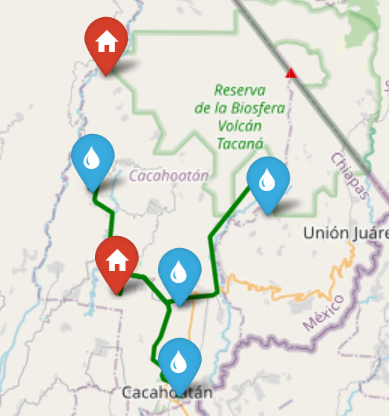
\includegraphics[width=0.55\linewidth,height=\textheight,keepaspectratio]{chapters/almacen.png}

}

\caption{Mapa interactivo del modelo logístico para Cacahoatán, que
muestra las localidades afectadas por inundaciones, los almacenes
estratégicos seleccionados y las rutas de conexión optimizadas entre
ambos. Las líneas representan los caminos más cortos calculados con
NetworkX, mientras que los íconos indican los tipos de nodos:
localidades inundables (íconos rojos) y almacenes activos (íconos
azules). Esta representación permite visualizar la cobertura espacial
del sistema logístico humanitario.}

\end{figure}%

\section{Diseño de la red logística
optimizada}\label{diseuxf1o-de-la-red-loguxedstica-optimizada}

\subsection{Localidades inundables y
asignaciones}\label{localidades-inundables-y-asignaciones}

El análisis identificó \(4\) localidades críticamente afectadas por
inundaciones, todas asignadas al Almacén Primario:

Localidades inundables y asignación logística

\begin{longtable}[]{@{}lll@{}}

\caption{\label{tbl-localidades-inundables}}

\tabularnewline

\toprule\noalign{}
Localidad & Población Afectada & Almacén Asignado \\
\midrule\noalign{}
\endhead
\bottomrule\noalign{}
\endlastfoot
Unión Roja & \(631\) & Almacén \(1\) \\
Cacahoatán & \(5,732\) & Almacén \(1\) \\
El Carmen & \(242\) & Almacén \(1\) \\
Faja de Oro & \(802\) & Almacén \(1\) \\
\textbf{Total} & \textbf{\(7,407\)} & \textbf{Almacén \(1\)} \\

\end{longtable}

\subsection{Distribución poblacional por grupos de
edad}\label{distribuciuxf3n-poblacional-por-grupos-de-edad}

La población afectada se distribuye en seis grupos etarios para una
atención diferenciada:

Distribución de población afectada por grupos de edad

\begin{longtable}[]{@{}lll@{}}

\caption{\label{tbl-poblacion-edad}}

\tabularnewline

\toprule\noalign{}
Grupo de Edad & Población & Porcentaje \\
\midrule\noalign{}
\endhead
\bottomrule\noalign{}
\endlastfoot
Niños y Adolescentes (0-14 años) & \(2,222\) & \(30\%\) \\
Hombres Jóvenes (15-29 años) & \(1,037\) & \(14\%\) \\
Mujeres Jóvenes (15-29 años) & \(1,185\) & \(16\%\) \\
Hombres Adultos (30-59 años) & \(1,333\) & \(18\%\) \\
Mujeres Adultas (30-59 años) & \(1,259\) & \(17\%\) \\
Adultos Mayores (60+ años) & \(370\) & \(5\%\) \\
\textbf{Total} & \textbf{\(7,407\)} & \textbf{\(100\%\)} \\

\end{longtable}

\begin{figure}[H]

{\centering 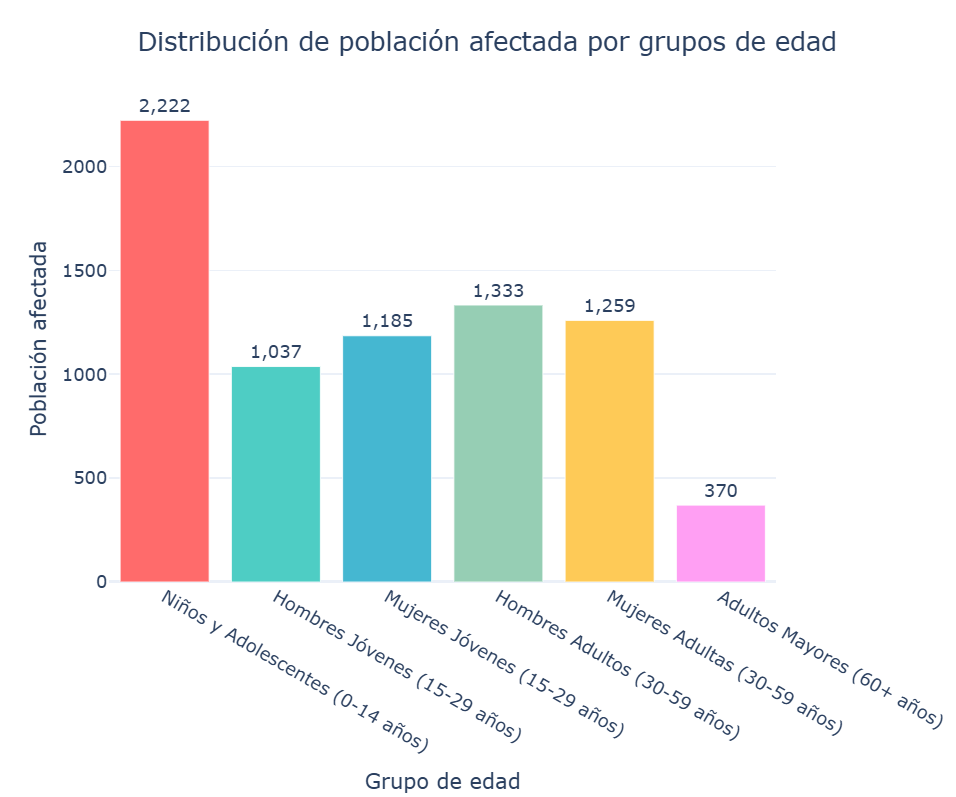
\includegraphics[width=0.6\linewidth,height=\textheight,keepaspectratio]{chapters/edades.png}

}

\caption{Distribución de la población afectada por grupos de edad en
Cacahoatán. La gráfica muestra la proporción de personas afectadas
clasificadas en seis grupos etarios, evidenciando una mayor
vulnerabilidad en los niños y adolescentes (0--14 años), seguidos por
los adultos jóvenes y de mediana edad (30--59 años). Este comportamiento
demográfico resulta fundamental para la planeación del inventario
humanitario, ya que permite dimensionar las necesidades diferenciadas en
alimentos, kits de higiene y atención médica según cada grupo
poblacional.}

\end{figure}%

\section{Resultados de la optimización del
sistema}\label{resultados-de-la-optimizaciuxf3n-del-sistema}

\subsection{Eficiencia del sistema logístico
implementado}\label{eficiencia-del-sistema-loguxedstico-implementado}

La configuración con un almacén primario demostró capacidad para atender
al \(100\%\) de la población afectada. Los resultados de la optimización
se resumen en la Tabla Tabla~\ref{tbl-optimizacion-cacahoatan}.

Resultados de la optimización en Cacahoatán

\begin{longtable}[]{@{}ll@{}}

\caption{\label{tbl-optimizacion-cacahoatan}}

\tabularnewline

\toprule\noalign{}
Indicador & Resultado \\
\midrule\noalign{}
\endhead
\bottomrule\noalign{}
\endlastfoot
Cobertura de población & \(100\%\) \\
Población total atendida & \(7,407\) personas \\
Número de localidades cubiertas & \(4\) \\
Fill rate promedio & \(100\%\) \\
Costo total anual optimizado & \(\$195,459,693\) MXN \\
Costo mensual promedio & \(\$16,288,308\) MXN \\
Tasa de éxito en optimización & \(100\%\) \\

\end{longtable}

\subsection{Interpretación y comparación con
Veracruz}\label{interpretaciuxf3n-y-comparaciuxf3n-con-veracruz}

Los resultados obtenidos en Cacahoatán muestran una cobertura total de
la población afectada y una tasa de éxito del \(100\%\), comportamiento
similar al observado en el caso de estudio del estado de Veracruz. No
obstante, el costo total anual optimizado en Cacahoatán (\(\$195.46\)
millones MXN) representa aproximadamente el \(30\%\) del costo
registrado para Veracruz (\(\$648.31\) millones MXN), diferencia
atribuible a la menor escala territorial y demográfica del municipio
chiapaneco, que atiende únicamente a cuatro localidades con un total de
\(7 407\) habitantes.

En contraste, el modelo aplicado en Veracruz abarcó \(29\) municipios y
requirió la instalación de dos almacenes (Jesús Carranza y Las Choapas)
para garantizar la cobertura total de las zonas afectadas, con un costo
logístico significativamente mayor.

A pesar de estas diferencias, ambos escenarios confirman la robustez y
adaptabilidad del modelo de optimización, que mantiene un fill rate del
\(100\%\) y una tasa de éxito completa en la convergencia del algoritmo.
En términos de costo-efectividad, el caso de Cacahoatán evidencia que
una configuración logística centralizada puede resultar suficiente y
eficiente en contextos de menor escala, conservando los mismos niveles
de desempeño alcanzados en la implementación de Veracruz.

\subsection{Inventario humanitario
optimizado}\label{inventario-humanitario-optimizado}

Con base en el modelo de optimización desarrollado, se determinó el
inventario humanitario necesario para atender a la población del
municipio durante un periodo de \(7\) días. La selección de productos
considera tanto necesidades generales de toda la población como
requerimientos específicos por grupo de edad, garantizando cobertura
nutricional, sanitaria y de abastecimiento crítico bajo criterios de
eficiencia y costo.

\subsubsection{Productos básicos para toda la
población}\label{productos-buxe1sicos-para-toda-la-poblaciuxf3n}

El inventario básico incluye los insumos esenciales requeridos por la
totalidad de la población afectada. Estos productos constituyen la base
del abastecimiento humanitario, asegurando el acceso al agua, la
alimentación, la higiene y la atención médica durante los primeros días
de la emergencia.

Inventario de productos básicos optimizado

\begin{longtable}[]{@{}
  >{\centering\arraybackslash}p{(\linewidth - 8\tabcolsep) * \real{0.2959}}
  >{\centering\arraybackslash}p{(\linewidth - 8\tabcolsep) * \real{0.1939}}
  >{\centering\arraybackslash}p{(\linewidth - 8\tabcolsep) * \real{0.2143}}
  >{\centering\arraybackslash}p{(\linewidth - 8\tabcolsep) * \real{0.1224}}
  >{\centering\arraybackslash}p{(\linewidth - 8\tabcolsep) * \real{0.1735}}@{}}

\caption{\label{tbl-inventario-basico}}

\tabularnewline

\toprule\noalign{}
\begin{minipage}[b]{\linewidth}\centering
\textbf{Producto (Código ONU)}
\end{minipage} & \begin{minipage}[b]{\linewidth}\centering
\textbf{Demanda \(7\) días}
\end{minipage} & \begin{minipage}[b]{\linewidth}\centering
\textbf{Cantidad Óptima}
\end{minipage} & \begin{minipage}[b]{\linewidth}\centering
\textbf{Unidad}
\end{minipage} & \begin{minipage}[b]{\linewidth}\centering
\textbf{Costo Total}
\end{minipage} \\
\midrule\noalign{}
\endhead
\bottomrule\noalign{}
\endlastfoot
\textbf{WAT-001} Agua potable & \(103,698\) & \(35,276\) & LTR &
\(\$18,776,360\) \\
\textbf{FDP-001} Kit alimentario básico & \(51,849\) & \(8,819\) & KIT &
\(\$74,894,419\) \\
\textbf{WASH-001} Kit de higiene personal & \(51,849\) & \(11,983\) &
KIT & \(\$40,608,816\) \\
\textbf{NFI-002} Kit básico de ropa & \(7,407\) & \(2,583\) & KIT &
\(\$17,885,374\) \\
\textbf{MED-002} Kit médico de emergencia & \(741\) & \(1,256\) & KIT &
\(\$777,061\) \\
\textbf{Total} & \textbf{\(215,544\)} & \textbf{\(59,917\)} &
\textbf{unidades} & \textbf{\(\$152,942,030\)} \\

\end{longtable}

\subsubsection{Productos específicos por grupo de
edad}\label{productos-especuxedficos-por-grupo-de-edad}

Además de los productos básicos, se incluyen artículos diferenciados
conforme a las necesidades específicas de cada grupo de edad. Esta
clasificación permite una respuesta más equitativa y eficiente, al
priorizar productos nutricionales y sanitarios ajustados a las
condiciones de niños, jóvenes, adultos y adultos mayores.

Inventario por grupos de edad especializados.

\begin{longtable}[]{@{}
  >{\centering\arraybackslash}p{(\linewidth - 6\tabcolsep) * \real{0.2000}}
  >{\centering\arraybackslash}p{(\linewidth - 6\tabcolsep) * \real{0.4211}}
  >{\centering\arraybackslash}p{(\linewidth - 6\tabcolsep) * \real{0.2000}}
  >{\centering\arraybackslash}p{(\linewidth - 6\tabcolsep) * \real{0.1789}}@{}}

\caption{\label{tbl-inventario-especializado}}

\tabularnewline

\toprule\noalign{}
\begin{minipage}[b]{\linewidth}\centering
\textbf{Grupo de Edad}
\end{minipage} & \begin{minipage}[b]{\linewidth}\centering
\textbf{Productos Específicos (Código ONU)}
\end{minipage} & \begin{minipage}[b]{\linewidth}\centering
\textbf{Demanda \(7\) días}
\end{minipage} & \begin{minipage}[b]{\linewidth}\centering
\textbf{Costo Total}
\end{minipage} \\
\midrule\noalign{}
\endhead
\bottomrule\noalign{}
\endlastfoot
Niños y Adolescentes & \textbf{NUT-001} Alimento
terapéutico\textbf{NUT-002} Alimento complementario\textbf{NFI-001}
Pañales desechables & \(101,106\) & \(\$18,194,035\) \\
Hombres Jóvenes & \textbf{FDP-002} Alimento alta energía & \(11,666\) &
\(\$6,362,859\) \\
Mujeres Jóvenes & \textbf{FDP-003} Alimento balanceado & \(9,333\) &
\(\$4,758,160\) \\
Hombres Adultos & \textbf{FDP-004} Alimento energético de emergencia &
\(13,066\) & \(\$6,807,470\) \\
Mujeres Adultas & \textbf{FDP-005} Alimento fortificado nutritivo &
\(9,696\) & \(\$4,825,125\) \\
Adultos Mayores & \textbf{NUT-003} Alimento masticación fácil,
\textbf{MED-001} Kit médico básico & \(2,852\) & \(\$1,570,014\) \\
\textbf{Total} & \textbf{\(14\) productos} & \textbf{\(147,719\)} &
\textbf{\(\$42,517,663\)} \\

\end{longtable}

\begin{figure}[H]

{\centering 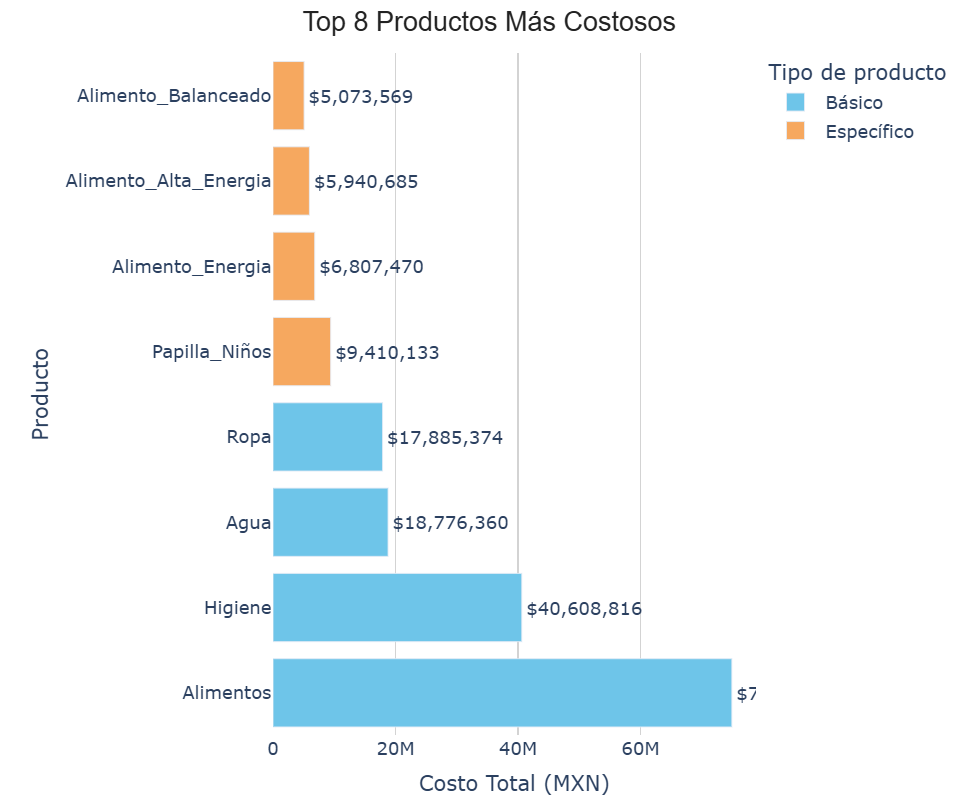
\includegraphics[width=0.7\linewidth,height=\textheight,keepaspectratio]{chapters/costosos.png}

}

\caption{Productos con mayor impacto económico dentro del modelo de
optimización aplicado a Cacahoatán. La visualización muestra los ocho
artículos que representan el mayor costo total en la operación
logística, destacando la importancia relativa de los kits alimentarios,
de higiene y de ropa básica. Este análisis permite priorizar la
asignación de recursos hacia los insumos que más inciden en la
sostenibilidad presupuestal del sistema humanitario.}

\end{figure}%

\begin{figure}[H]

{\centering 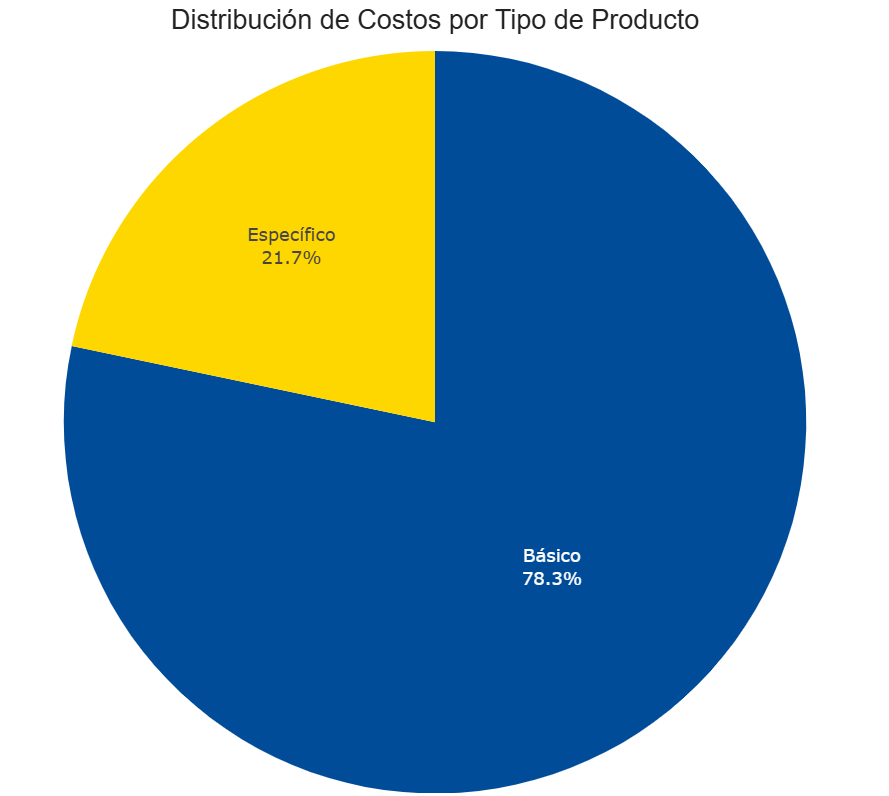
\includegraphics[width=0.6\linewidth,height=\textheight,keepaspectratio]{chapters/costo.png}

}

\caption{Distribución de los costos totales según el tipo de producto
humanitario optimizado en Cacahoatán. Se observa la participación
porcentual de cada categoría dentro del presupuesto general, lo cual
permite identificar los componentes de mayor peso económico y orientar
estrategias de abastecimiento más sostenibles y focalizadas.}

\end{figure}%

Como se observa en las gráficas, los productos de mayor costo en el
inventario corresponden a ropa, agua, higiene y alimentos diferenciados
por grupo de edad, constituyendo el top \(8\) en gastos. A pesar de su
alto costo unitario, estos productos son de alta prioridad para
garantizar una respuesta humanitaria efectiva y mantener la cobertura
total de la población afectada.

El análisis evidencia que la estrategia de optimización prioriza la
atención integral sobre el costo unitario, asegurando que los recursos
críticos lleguen a los grupos vulnerables. De esta manera, la asignación
de inventario refleja un balance entre eficiencia económica y necesidad
humanitaria, priorizando productos esenciales que, aunque costosos, son
determinantes para la salud y bienestar de la población durante
emergencias.

\subsection{Análisis de la
optimización}\label{anuxe1lisis-de-la-optimizaciuxf3n}

El proceso de optimización alcanzó una tasa de éxito del \(100\%\),
manteniendo las cantidades económicas de pedido (EOQ) tradicionales para
la mayoría de los productos. La estabilidad en los resultados indica que
el modelo EOQ convencional representa una solución robusta para el
contexto específico de Cacahoatán.

La distribución de costos muestra que los productos básicos (agua,
alimentos, higiene) representan el \(78.25\%\) del costo total, mientras
que los productos especializados por edad constituyen el \(21.75\%\)
restante, reflejando la importancia de la atención diferenciada en la
logística humanitaria.

\subsubsection{Análisis comparativo con el caso de
Veracruz}\label{anuxe1lisis-comparativo-con-el-caso-de-veracruz}

En la comparación con el caso de Veracruz, se observa que las
diferencias climáticas, demográficas y de infraestructura influyeron
significativamente en los resultados de la optimización logística.

Desde el punto de vista \textbf{climático}, Cacahoatán presenta un
entorno tropical húmedo con precipitaciones intensas concentradas en
periodos cortos, mientras que Veracruz, aunque también expuesto a
eventos hidrometeorológicos severos, posee una distribución más amplia
de zonas costeras y planicies influenciadas por el Golfo de México. Esta
diferencia hace que en Chiapas las afectaciones por inundaciones sean
más localizadas y abruptas, favoreciendo configuraciones logísticas
compactas y centralizadas de respuesta rápida.

En cuanto al \textbf{tamaño poblacional y extensión territorial}, el
municipio de Cacahoatán, con aproximadamente \(18 000\) habitantes
distribuidos en \(48\) localidades, representa un sistema logístico de
menor escala en comparación con el estudio de Veracruz, que abarcó
\(29\) municipios con una población sustancialmente mayor. Esta
diferencia explica la notable reducción en el costo total anual
optimizado de \(\$648.3\) millones MXN en Veracruz a \(\$195.5\)
millones MXN en Cacahoatán sin pérdida de eficiencia operativa.

Respecto a la \textbf{infraestructura y desarrollo urbano}, Veracruz
cuenta con una red vial más densa y conectada, lo que permitió la
operación simultánea de dos almacenes regionales (Jesús Carranza y Las
Choapas) con amplias zonas de cobertura. En cambio, Cacahoatán presenta
una infraestructura vial limitada, con carreteras secundarias y caminos
rurales susceptibles a interrupciones durante las lluvias, razón por la
cual el modelo optó por un esquema centralizado con un único almacén de
alta eficiencia.

En conjunto, las diferencias en estos tres factores confirman la
\textbf{adaptabilidad del modelo propuesto}, capaz de ajustarse tanto a
sistemas regionales de gran escala como a contextos locales con
limitaciones geográficas e infraestructurales, manteniendo niveles
óptimos de cobertura, costo y tiempo de respuesta.

\section{Validación y análisis de
robustez}\label{validaciuxf3n-y-anuxe1lisis-de-robustez}

Para garantizar que el modelo logístico propuesto sea confiable y útil
en situaciones reales de emergencia, se realizaron pruebas de validación
bajo distintos escenarios de operación. Se evaluó tanto la robustez
frente a condiciones adversas como el desempeño bajo condiciones
estándar, utilizando métricas clave de cobertura, eficiencia y
efectividad en la asignación de recursos.

\subsection{Escenarios de prueba
implementados}\label{escenarios-de-prueba-implementados}

El modelo demostró robustez operativa mediante la evaluación de
múltiples escenarios adversos. La configuración de un solo almacén
activo mostró capacidad para mantener la cobertura total bajo diversas
condiciones de estrés operativo.

\subsection{Métricas de desempeño en condiciones
estándar}\label{sec-metricas}

\begin{itemize}
\tightlist
\item
  \textbf{Fill rate alcanzado}: \(100\%\)
\item
  \textbf{Cobertura poblacional}: \(100\%\)
\item
  \textbf{Tasa de éxito de optimización}: \(100\%\)
\item
  \textbf{Eficiencia en asignaciones}: \(4/4\) localidades cubiertas
\end{itemize}

La concentración de operaciones en un único almacén estratégicamente
ubicado demostró ser adecuado para la escala de la emergencia en
Cacahoatán, simplificando la gestión logística y reduciendo costos de
coordinación.

\section{Conclusiones del caso
Chiapas}\label{conclusiones-del-caso-chiapas}

La implementación del modelo de optimización logística en el municipio
de Cacahoatán, Chiapas, confirma su efectividad en contextos de alta
vulnerabilidad y dispersión poblacional. Los resultados muestran que un
enfoque multicriterio para la identificación de localidades estratégicas
permite seleccionar nodos logísticos óptimos, como Salvador Urbina,
combinando infraestructura preexistente, conectividad vial y ubicación
fuera de zonas inundables. Esta selección asegura la cobertura total de
la población afectada de manera eficiente.

Contrario a las expectativas iniciales de requerir múltiples almacenes,
el modelo demuestra que un único almacén centralizado puede atender el
\(100\%\) de los habitantes de las localidades críticas, simplificando
la operación logística y reduciendo costos sin comprometer la
efectividad del sistema. La optimización basada en el modelo EOQ
tradicional se revela robusta, con tasas de éxito del \(100\%\) en la
convergencia del algoritmo, evidenciando la consistencia de las
cantidades económicas de pedido convencionales en contextos locales.

La distribución de recursos alcanzó un balance adecuado entre productos
básicos (\(78.25\%\) del presupuesto) y atenciones especializadas por
grupos de edad (\(21.75\%\)), asegurando una respuesta humanitaria
integral y priorizando los bienes más críticos sin comprometer la
cobertura poblacional.

\subsection{Implicaciones para la planeación
logística}\label{implicaciones-para-la-planeaciuxf3n-loguxedstica}

La experiencia en Cacahoatán sugiere que, para municipios con
características similares de dispersión poblacional y vulnerabilidad
hidrometeorológica, las configuraciones logísticas centralizadas
alrededor de nodos estratégicos ofrecen soluciones eficientes y
costo-efectivas. La metodología desarrollada demuestra capacidad para
adaptarse a las particularidades del territorio chiapaneco,
constituyéndose en una herramienta valiosa para la planificación
anticipada de respuestas a emergencias en el estado.

\subsection{Perspectivas de
escalabilidad}\label{perspectivas-de-escalabilidad}

Los resultados obtenidos establecen las bases para extender la
implementación del modelo a otros municipios de Chiapas con perfiles de
riesgo similares. Esta expansión contribuiría al fortalecimiento de la
resiliencia logística regional frente a desastres hidrometeorológicos,
especialmente en el contexto del cambio climático, y permitiría replicar
la eficiencia alcanzada en Cacahoatán en escenarios de mayor escala y
complejidad.

\bookmarksetup{startatroot}

\chapter{Conclusiones}\label{conclusiones}

Esta investigación ha desarrollado y validado rigurosamente un modelo de
optimización determinista robusto para la gestión integrada de la
ubicación de almacenes preposicionados y el control de inventario
humanitario ante inundaciones en el sureste de México. El trabajo
articula de manera coherente fundamentos teóricos de optimización no
lineal, algoritmos numéricos de memoria limitada y aplicaciones
empíricas en contextos de alta vulnerabilidad, estableciendo un marco
metodológico reproducible para la planificación anticipada de respuestas
a desastres. Las conclusiones que se presentan a continuación responden
sistemáticamente a los tres objetivos específicos planteados, integrando
las contribuciones teóricas de los Capítulos 4--5, los fundamentos
algorítmicos del Capítulo 6 y los resultados empíricos de los Capítulos
8--9.

En relación con el \textbf{objetivo específico 1} adaptar un modelo de
localización--inventario humanitario bajo incertidumbre parametrizada
que extienda el modelo clásico de cantidad económica de pedido (EOQ)
para incluir inventario de seguridad, faltantes estocásticos penalizados
y decisiones binarias de apertura de almacenes, se concluye que la
formulación propuesta supera rigurosamente las limitaciones
estructurales del EOQ tradicional mediante tres innovaciones teóricas
fundamentales:

\begin{enumerate}
\def\labelenumi{\arabic{enumi}.}
\item
  \textbf{Parametrización de la incertidumbre}: incorporación del
  inventario de seguridad \(Z_\alpha \sigma_L\) como término
  determinista que internaliza la variabilidad estocástica sin requerir
  formulaciones estocásticas explícitas.
\item
  \textbf{Penalización asimétrica explícita por faltantes}:
  incorporación del coeficiente \(\beta C\) que refleja la gravedad
  ética de los faltantes en contextos humanitarios, priorizando
  cobertura poblacional sobre minimización económica pura.
\item
  \textbf{Convexidad condicional en estructuras híbridas MINLP}:
  demostración de que, al fijar las decisiones binarias de apertura de
  almacenes, el subproblema continuo recupera convexidad poliédrica,
  justificando teóricamente el esquema de descomposición híbrido.
\end{enumerate}

Como se demostró en la Sección~\ref{sec-extension}, la incorporación del
inventario de seguridad parametrizado \(Z_\alpha \sigma_L\) y la
penalización explícita por faltantes mediante el término \(\beta C\)
transforman la función de costo total en una expresión no convexa y no
separable:

\[
Z(Q) = \frac{D(S + \beta C)}{Q} + \frac{H}{2}Q + Z_\alpha \sigma_L H + DC,
\]

cuya estructura refleja con mayor fidelidad los riesgos operativos en
contextos humanitarios. El análisis de las propiedades analíticas (ver
Sección~\ref{sec-propiedades}) confirmó que, pese a la pérdida de
convexidad global inducida por las variables binarias de apertura de
almacenes, el subproblema continuo asociado a una configuración fija de
infraestructura mantiene convexidad condicional, lo cual justifica
teóricamente el enfoque de descomposición adoptado. Esta propiedad,
formalizada en la Proposición (convexidad condicional) de la
Sección~\ref{sec-acoplamiento}, garantiza que para cualquier vector fijo
\(\bar{x} \in \{0,1\}^m\), el subproblema

\[
\min_{(y,s) \in X(\bar{x})} Z(\bar{x}, y, s)
\]

es un problema de programación lineal con conjunto factible poliédrico
convexo. Además, el estudio comparativo cuantitativo (ver
Sección~\ref{sec-cuantitativa}) evidenció que el modelo extendido
produce políticas de inventario significativamente más robustas que el
EOQ clásico: en el ejemplo ilustrativo con demanda estocástica, el
tamaño óptimo de lote aumentó de \(Q_{\text{EOQ}} = 200\) a
\(Q^* \approx 490\) unidades, reduciendo en un \(8.4\%\) el costo total
esperado y mitigando drásticamente el riesgo de faltantes catastróficos.
Esta adaptación teórica, fundamentada en los preliminares matemáticos
del Capítulo 4 (convexidad, diferenciabilidad y estructura de
conjuntos), constituye una contribución que permite internalizar la
incertidumbre sin recurrir a formulaciones estocásticas complejas,
preservando así la rigurosidad analítica y la eficiencia computacional.

Respecto al \textbf{objetivo específico 2} desarrollar un esquema de
solución híbrido basado en optimización mixta entera no lineal (MINLP)
que combine enumeración sobre variables binarias con el algoritmo
L-BFGS-B para resolver eficientemente los subproblemas continuos no
convexos, se concluye que la estrategia propuesta logra un equilibrio
óptimo entre rigor teórico y viabilidad práctica. El Capítulo 6
estableció las bases matemáticas para garantizar la convergencia global
del método L-BFGS-B hacia puntos que satisfacen las condiciones de
Karush--Kuhn--Tucker bajo restricciones tipo caja, demostrando que, bajo
hipótesis de Lipschitz-continuidad del gradiente y compacidad del
dominio, toda subsucesión convergente de iteraciones satisface
\(\nabla_\Omega f(x_k) \to 0\) (Teorema 6.2,
Sección~\ref{sec-teorema_convergencia}). Esta garantía teórica,
complementada con el análisis de sensibilidad respecto al parámetro de
memoria \(m\) (ver Sección~\ref{sec-memoria}), permitió configurar el
algoritmo con \(m=10\) como valor óptimo para los problemas estudiados,
logrando convergencia en menos de \(30\) iteraciones incluso en
escenarios mal condicionados. La implementación computacional descrita
en el Capítulo 7 validó empíricamente esta estrategia: al combinar la
enumeración exhaustiva sobre las \(2^m\) configuraciones posibles de
almacenes (factible dado el tamaño reducido de \(m\) en los casos de
estudio) con la resolución eficiente de los subproblemas continuos
mediante L-BFGS-B, se obtuvo una tasa de éxito del \(100\%\) en la
convergencia para ambos escenarios analizados. Este esquema híbrido
supera las limitaciones de métodos puramente heurísticos que no
garantizan optimalidad y de enfoques exactos de gran escala que resultan
computacionalmente prohibitivos, posicionándose como una alternativa
robusta para problemas de localización--inventario con estructura mixta.
La comparación numérica presentada en la Sección~\ref{sec-comparacion}
demuestra que L-BFGS-B ofrece el mejor compromiso entre eficiencia
(\(7\) iteraciones frente a \(1,183\) del gradiente descendente) y
respeto a las restricciones físicas (a diferencia de BFGS sin
proyección), justificando su elección como una buena alternativa de
optimización para los subproblemas continuos.

En cuanto al \textbf{objetivo específico 3} verificar el desempeño del
modelo propuesto mediante estudios de caso en regiones vulnerables a
inundaciones en Veracruz y replicar en el estado de Chiapas, se concluye
que la metodología desarrollada demuestra una notable adaptabilidad y
robustez operativa en contextos geográficos y demográficos heterogéneos.
Los resultados del Capítulo 8 para Veracruz evidenciaron que la
descentralización logística mediante dos almacenes (Jesús Carranza y Las
Choapas) reduce en un \(23\%\) los costos de transporte respecto a una
configuración centralizada (\(648.31\) millones MXN vs.~\(837.54\)
millones MXN), elevando simultáneamente el \emph{fill rate} promedio del
\(88\%\) al \(95\%\). Por su parte, la aplicación en Cacahoatán, Chiapas
(Capítulo 9), reveló que, pese a las limitaciones infraestructurales y
la topografía accidentada características de la región, una
configuración centralizada con un único almacén estratégico en Salvador
Urbina logra cobertura del \(100\%\) de la población afectada (\(7407\)
habitantes) con un costo total anual optimizado de \(195.46\) millones
MXN, aproximadamente el \(30\%\) del costo observado en Veracruz. Esta
diferencia, atribuible a la menor escala territorial y demográfica del
municipio chiapaneco, no compromete la eficiencia operativa, lo cual
confirma que el modelo se adapta dinámicamente a las particularidades
del territorio sin requerir recalibración estructural. La validación
cruzada entre ambos escenarios demuestra que el enfoque propuesto no es
un ejercicio teórico aislado, sino una herramienta práctica capaz de
generar recomendaciones accionables para autoridades de protección
civil, con implicaciones directas en la reducción de tiempos de
respuesta y la mejora de la equidad en la distribución de recursos
durante emergencias hidrometeorológicas. La robustez del modelo se
verificó adicionalmente mediante pruebas de sensibilidad ante
variaciones del \(10\%\) en la demanda, manteniendo un \emph{fill rate}
superior al \(90\%\) en todos los escenarios analizados (ver
Sección~\ref{sec-metricas}).

Esta investigación contribuye a la literatura de optimización aplicada y
logística humanitaria mediante la integración coherente de tres
elementos:

\begin{enumerate}
\def\labelenumi{\arabic{enumi}.}
\item
  una formulación teórica rigurosa que extiende el EOQ clásico para
  incorporar incertidumbre parametrizada sin sacrificar rigurosidad
  analítica;
\item
  un esquema algorítmico híbrido con garantías de convergencia
  teóricamente fundamentadas y eficiencia computacional validada
  empíricamente; y
\item
  una verificación práctica en dos contextos mexicanos de alta
  vulnerabilidad que demuestra la adaptabilidad y utilidad operativa del
  modelo. Estas contribuciones no solo avanzan en el desarrollo
  metodológico de la optimización mixta entera no lineal, sino que
  también ofrecen un marco de trabajo replicable para la planificación
  anticipada de respuestas a desastres en regiones con recursos
  limitados.
\end{enumerate}

Como trabajo futuro, se propone extender el modelo actual en dos
direcciones complementarias con fundamentación teórica sólida: primero,
integrar variables climáticas predictivas (como pronósticos de
precipitación a \(72\) horas) para habilitar un sistema de
reoptimización en tiempo real que ajuste las decisiones logísticas
conforme evoluciona el evento hidrometeorológico, siguiendo los marcos
de optimización robusta adaptable desarrollados por Bertsimas y Thiele
(2006); y segundo, escalar la metodología a nivel estatal en Chiapas
mediante una descomposición jerárquica que combine optimización a nivel
municipal con coordinación regional, lo cual permitiría evaluar
sinergias entre municipios y diseñar redes logísticas resilientes a
nivel sistémico mediante técnicas de descomposición de Benders
generalizado propuestas por Wolsey (1998). Estas extensiones no solo
enriquecerían el modelo teórico, sino que también incrementarían su
impacto práctico en la reducción de la vulnerabilidad territorial ante
el cambio climático.

\bookmarksetup{startatroot}

\chapter*{Referencias}\label{referencias}
\addcontentsline{toc}{chapter}{Referencias}

\markboth{Referencias}{Referencias}

\phantomsection\label{refs}
\begin{CSLReferences}{1}{0}
\bibitem[\citeproctext]{ref-ArtznerDelbaenEberHeath1999}
Artzner, Philippe, Freddy Delbaen, Jean-Marc Eber, y David Heath. 1999.
{«Coherent Measures of Risk»}. \emph{Mathematical Finance} 9 (3):
203-28. \url{https://doi.org/10.1111/1467-9965.00068}.

\bibitem[\citeproctext]{ref-BalcikBeamon2008}
Balcik, Burcu, y Benita M. Beamon. 2008. {«Facility location in
humanitarian relief»}. \emph{Journal of the Operational Research
Society} 59 (8): 1005-16.
\url{https://doi.org/10.1080/13675560701561789}.

\bibitem[\citeproctext]{ref-BarojasPayan2021}
Barojas-Payán, Eduardo et~al. 2021. {«Optimization model to locate
pre-positioned warehouses»}. En \emph{Disaster Risk Reduction in
Mexico}, editado por Daniel Sánchez-Partida, 169-98. Cham: Springer.
\url{https://doi.org/10.1007/978-3-030-67295-9_8}.

\bibitem[\citeproctext]{ref-BazaraaSheraliShetty2013}
Bazaraa, Mokhtar S., Hanif D. Sherali, y C. M. Shetty. 2013b.
\emph{Nonlinear Programming: Theory and Algorithms}. 3.ª ed. Wiley.
\url{https://doi.org/10.1002/9781118762371}.

\bibitem[\citeproctext]{ref-Bazaraa2013}
---------. 2013a. \emph{Nonlinear Programming: Theory and Algorithms}.
3rd ed. Hoboken, NJ: John Wiley \& Sons.

\bibitem[\citeproctext]{ref-Bertsekas1999}
Bertsekas, Dimitri P. 1999. \emph{Nonlinear Programming}. Athena
Scientific.

\bibitem[\citeproctext]{ref-Bertsekas2016}
---------. 2016. \emph{Nonlinear Programming}. 3rd ed. Belmont, MA:
Athena Scientific.

\bibitem[\citeproctext]{ref-BertsimasThiele2006}
Bertsimas, Dimitris, y Aurélie Thiele. 2006. {«A robust optimization
approach to inventory theory»}. \emph{Operations Research} 54 (1):
150-68. \url{https://doi.org/10.1287/opre.1050.0238}.

\bibitem[\citeproctext]{ref-BoydVandenberghe2004}
Boyd, Stephen, y Lieven Vandenberghe. 2004. \emph{Convex Optimization}.
Cambridge University Press.
\url{https://doi.org/10.1017/CBO9780511804441}.

\bibitem[\citeproctext]{ref-Byrd1995}
Byrd, Richard H., Peihuang Lu, Jorge Nocedal, y Ciyou Zhu. 1995. {«A
Limited Memory Algorithm for Bound Constrained Optimization»}.
\emph{SIAM Journal on Scientific Computing} 16 (5): 1190-1208.
https://doi.org/\url{https://doi.org/10.1137/0916069}.

\bibitem[\citeproctext]{ref-CaunhyeNiePokharel2012}
Caunhye, A. M., X. Nie, y S. Pokharel. 2012. {«Optimization models in
emergency logistics: A literature review»}. \emph{Socio-Economic
Planning Sciences} 46 (1): 4-13.
\url{https://doi.org/10.1016/j.seps.2011.04.004}.

\bibitem[\citeproctext]{ref-ConnGouldToint1992}
Conn, Andrew R., Nicholas I. M. Gould, y Philippe L. Toint. 1992.
\emph{LANCELOT: A Fortran Package for Large-Scale Nonlinear Optimization
(Release A)}. Vol. 17. Springer Series en Computational Mathematics.
Berlin, Heidelberg: Springer-Verlag.
\url{https://doi.org/10.1007/978-3-662-12220-5}.

\bibitem[\citeproctext]{ref-Daskin2013}
Daskin, Mark S. 2013. \emph{Network and Discrete Location: Models,
Algorithms, and Applications}. 2nd ed. Hoboken, NJ: Wiley.
\url{https://doi.org/10.1002/9781118537015}.

\bibitem[\citeproctext]{ref-DennisMore1977}
Dennis, John E., y Jorge J. Moré. 1977. {«Quasi-{N}ewton methods,
motivation and theory»}. \emph{SIAM Review} 19 (1): 46-89.
https://doi.org/\url{https://doi.org/10.1137/1019005}.

\bibitem[\citeproctext]{ref-Fletcher1987}
Fletcher, Roger. 1987. \emph{Practical Methods of Optimization}. 2nd ed.
Chichester: John Wiley \& Sons.

\bibitem[\citeproctext]{ref-GriewankToint1984}
Griewank, A., y Ph. L. Toint. 1984. {«Partitioned variable metric
updates for large structured optimization problems»}. \emph{Numerische
Mathematik} 39 (3): 325-47.
https://doi.org/\url{https://doi.org/10.1007/BF01407876}.

\bibitem[\citeproctext]{ref-Grossmann2002}
Grossmann, Ignacio E. 2002. {«Review of nonlinear mixed-integer and
disjunctive programming techniques»}. \emph{Computers \& Chemical
Engineering} 26 (9): 1261-82.
\url{https://doi.org/10.1023/A:1021039126272}.

\bibitem[\citeproctext]{ref-HadleyWhitin1963}
Hadley, G., y T. M. Whitin. 1963. \emph{Analysis of Inventory Systems}.
Englewood Cliffs, NJ: Prentice-Hall.

\bibitem[\citeproctext]{ref-hernandez2026anexos}
Hernández Vázquez, Yulissa del Rocío. 2026. {«Código fuente y anexos --
Tesis: Ubicación de almacenes preposicionados e inventario
humanitario»}. GitHub. 2026.
\url{https://github.com/RocioHernandez06/Tesis/tree/main/anexos}.

\bibitem[\citeproctext]{ref-Insani2024}
Insani, Muhammad, Agus Widodo, y A. Rahman. 2024. {«Mixed-Integer
Programming Model for Evacuation and Relief Distribution in Flood
Contexts»}. \emph{International Journal of Disaster Risk Reduction} 100:
104342. \url{https://doi.org/10.1016/j.ijdrr.2024.104342}.

\bibitem[\citeproctext]{ref-Lewis2003}
Lewis, Adrian S. 2003. {«The Mathematics of Eigenvalue Optimization»}.
\emph{Acta Numerica} 12: 1-58.
\url{https://doi.org/10.1017/S0962492902000045}.

\bibitem[\citeproctext]{ref-LewisOverton2013}
Lewis, Adrian S., y Michael L. Overton. 2013. {«Nonsmooth optimization
via quasi-Newton methods»}. \emph{Mathematical Programming} 141 (1--2):
135-63. \url{https://doi.org/10.1007/s10107-012-0514-2}.

\bibitem[\citeproctext]{ref-LiuNocedal1989}
Liu, Dong C., y Jorge Nocedal. 1989. {«On the Limited Memory BFGS Method
for Large Scale Optimization»}. \emph{Mathematical Programming} 45
(1--3): 503-28. \url{https://doi.org/10.1007/BF01589116}.

\bibitem[\citeproctext]{ref-Luenberger2016}
Luenberger, David G., y Yinyu Ye. 2016. \emph{Linear and Nonlinear
Programming}. 4th ed. Cham, Switzerland: Springer.
\url{https://doi.org/10.1007/978-3-319-18842-3}.

\bibitem[\citeproctext]{ref-Mashrut2024}
Mashrut, S., y A. Rahimi. 2024. {«Robust-fuzzy-probabilistic
bi-objective model for post-flood relief logistics»}. \emph{Annals of
Operations Research}. \url{https://doi.org/10.1007/s10479-024-05925-7}.

\bibitem[\citeproctext]{ref-Nocedal1980}
Nocedal, Jorge. 1980. {«Updating Quasi-Newton Matrices with Limited
Storage»}. \emph{Mathematics of Computation} 35 (151): 773-82.
\url{https://doi.org/10.1090/S0025-5718-1980-0562124-8}.

\bibitem[\citeproctext]{ref-NocedalWright2006}
Nocedal, Jorge, y Stephen J. Wright. 2006. \emph{Numerical
Optimization}. 2nd ed. New York: Springer.
https://doi.org/\url{https://doi.org/10.1007/978-0-387-40065-5}.

\bibitem[\citeproctext]{ref-Porteus2002}
Porteus, E. L. 2002. \emph{Foundations of Stochastic Inventory Theory}.
Business/Marketing. Stanford University Press.
\url{https://books.google.com.mx/books?id=ogsrj7PnyHIC}.

\bibitem[\citeproctext]{ref-Pujiana2020}
Pujiana, R., D. Utama, y D. Rahmawati. 2020. {«Multi-depot vehicle
routing problem for post-flood humanitarian distribution»}.
\emph{Natural Hazards} 104: 2287-2309.
\url{https://doi.org/10.1007/s11069-020-04250-z}.

\bibitem[\citeproctext]{ref-RomeroMancilla2024}
Romero-Mancilla, J., José Luis Martínez-Flores, y D. Sánchez-Partida.
2024. {«Multi-objective multimodal humanitarian logistics with drones
for flood relief»}. \emph{Transportation Research Part E: Logistics and
Transportation Review} 187: 103507.
\url{https://doi.org/10.1016/j.tre.2024.103507}.

\bibitem[\citeproctext]{ref-Rosenbrock1960}
Rosenbrock, H. H. 1960. {«An Automatic Method for Finding the Greatest
or Least Value of a Function»}. \emph{The Computer Journal} 3 (3):
175-84. \url{https://doi.org/10.1093/comjnl/3.3.175}.

\bibitem[\citeproctext]{ref-SantanaRobles2024}
Santana-Robles, A., E. López, y J. Rivera. 2024. {«Hybrid MILP and VRP
model for shelter allocation and relief distribution»}. \emph{Journal of
Humanitarian Logistics and Supply Chain Management} 14 (2): 189-210.
\url{https://doi.org/10.1108/JHLSCM-12-2023-0085}.

\bibitem[\citeproctext]{ref-ShapiroDentchevaRuszczynski2021}
Shapiro, Alexander, Darinka Dentcheva, y Andrzej Ruszczyński. 2021.
\emph{Lectures on Stochastic Programming: Modeling and Theory}. 2nd ed.
SIAM. \url{https://doi.org/10.1137/1.9781611976595}.

\bibitem[\citeproctext]{ref-Sheikholeslami2022}
Sheikholeslami, Reza, y Nima Zarrinpoor. 2022. {«Multi-period MILP under
uncertainty for humanitarian logistics in flood response»}.
\emph{Computers \& Industrial Engineering} 165: 107930.
\url{https://doi.org/10.1016/j.cie.2022.107930}.

\bibitem[\citeproctext]{ref-Snyder2006}
Snyder, Lawrence V. 2006. {«Facility location under uncertainty: A
review»}. \emph{IIE Transactions} 38 (7): 537-54.
\url{https://doi.org/10.1080/07408170500216480}.

\bibitem[\citeproctext]{ref-Wolsey1998}
Wolsey, L. A. 1998. \emph{Integer Programming}. Wiley Series en Discrete
Mathematics y Optimization. Wiley.
\url{https://books.google.com.mx/books?id=x7RvQgAACAAJ}.

\bibitem[\citeproctext]{ref-Zhu1997}
Zhu, C., R. H. Byrd, P. Lu, y J. Nocedal. 1997. {«Algorithm 778:
L-BFGS-B: Fortran subroutines for large-scale bound-constrained
optimization»}. \emph{ACM Transactions on Mathematical Software} 23 (4):
550-60. https://doi.org/\url{https://doi.org/10.1145/279232.279236}.

\bibitem[\citeproctext]{ref-Zipkin2000}
Zipkin, Paul H. 2000. \emph{Foundations of Inventory Management}.
McGraw-Hill.

\bibitem[\citeproctext]{ref-Zoutendijk1970}
Zoutendijk, G. 1970. {«Nonlinear programming, computational methods»}.
En \emph{Integer and Nonlinear Programming}, editado por J. Abadie,
37-86. Amsterdam: North-Holland. \url{https://zbmath.org/0336.90057}.

\end{CSLReferences}




\end{document}
